\documentclass[11pt,a4paper,twoside]{book} %scrbook book report
\usepackage{hyperref}  % Necesario para manejar los enlaces
\usepackage[
backend=biber,
style=apa,
% sorting=ynt
backref=true,         % Habilitar backref
backrefstyle=none,    % Controla el formato de las referencias a las páginas
hyperref=true,         % Habilitar hyperref
]{biblatex}

\addbibresource{own-bib.bib}
\addbibresource{thesis_references.bib}
\addbibresource{laser-references.bib}


% Configuración de hyperref
\hypersetup{
	colorlinks=true,    % Habilita el coloreado de los enlaces
	linkcolor=blue,     % Color de los enlaces internos
	citecolor=blue,     % Color de las citas
	urlcolor=blue       % Color de los enlaces externos
}


% Essential packages
\usepackage{amsmath, amssymb, amsthm} % AMS Packages
\usepackage{graphicx,color}           % Packages for graphics and color
\usepackage{geometry}
\PassOptionsToPackage{printonlyused,smaller}{acronym}
\usepackage{acronym}
% Optional customization packages
\usepackage{lmodern}                  % Custom fonts
\usepackage[T1]{fontenc}              % Ensure correct font encoding
\usepackage{mathptmx}              % Times New Roman Font accross the document

\usepackage{subfigure}
%\usepackage{subcaption}
\usepackage{wrapfig}
\usepackage{multirow}

\usepackage{multicol}

\usepackage{url}

\usepackage{listings}

%\usepackage{xcolor}

\definecolor{codegreen}{rgb}{0,0.6,0}
\definecolor{codegray}{rgb}{0.5,0.5,0.5}
\definecolor{codepurple}{rgb}{0.58,0,0.82}
\definecolor{backcolour}{rgb}{0.95,0.95,0.92}

\lstdefinestyle{mystyle}{
	backgroundcolor=\color{backcolour},   
	commentstyle=\ttfamily\color{codegreen},
	keywordstyle=\color{magenta},
	numberstyle=\tiny\color{codegray},
	stringstyle=\color{codepurple},
	basicstyle=\footnotesize,
	breakatwhitespace=false,         
	breaklines=true,                 
	captionpos=b,                    
	keepspaces=true,                 
	numbers=left,                    
	numbersep=5pt,                  
	showspaces=false,                
	showstringspaces=false,
	showtabs=false,                  
	tabsize=2
}


\lstset{style=mystyle}
\lstset{language=Python}

% Customising chapter headings - sectsty.pdf
\usepackage{sectsty}
\chapterfont{\Large\sc\centering}
\chaptertitlefont{\centering}
\subsubsectionfont{\centering}

\usepackage[hang, small, bf, margin=0pt, tableposition=bottom]{caption}
\setlength{\abovecaptionskip}{10pt}   % Custom captions

\captionsetup{
	justification=justified, % Center the caption label and first line
	format=plain, % Standard format
	singlelinecheck=false, % Disable single line centering
	indention=0pt
}

% Tables
\usepackage[table]{xcolor}
\usepackage{colortbl}

\usepackage{todonotes}

\newcommand{\mc}[2]{\multicolumn{#1}{c}{#2}}
\definecolor{Gray}{gray}{0.83}

\newcolumntype{x}{>{\columncolor{Gray}}c}
\newcolumntype{y}{>{\columncolor{white}}c}

% Page layout
\parindent 0pt
\parskip 1ex
\renewcommand{\baselinestretch}{1.49}
\numberwithin{equation}{section}
\renewcommand{\bibname}{References}
\renewcommand{\contentsname}{Contents}
\pagenumbering{roman}


\newcommand{\acrolabel}[1]{\makebox[3cm][l]{\textbf{#1}}}
\newenvironment{acronyms}{\begin{list}{}{\renewcommand{\makelabel}{\acrolabel}}}{\end{list}}

% \includeonly{tex/chapter1}          % Option to generate specific chapters

% Customising headers - fancyhdr.pdf
\usepackage{fancyhdr}
\pagestyle{fancy}
\rhead{}
\lhead{\nouppercase{\textsc{\leftmark}}}
\renewcommand{\headrulewidth}{0pt}
\makeatletter
\renewcommand{\chaptermark}[1]{\markboth{\textsc{\@chapapp}\ \thechapter:\ #1}{}}
\makeatother


% Hyperreferencing and citations
\usepackage{hyperref}
\hypersetup{
	colorlinks,
	citecolor=blue,
	filecolor=blue,
	linkcolor=blue,
	urlcolor=blue
}

% Section symbol
\usepackage{cleveref}
\crefname{section}{\S}{\S\S}
\Crefname{section}{\S}{\S\S}
\crefname{subsection}{\S}{\S\S}
\Crefname{subsection}{\S}{\S\S}

% packages from lymnaea paper
\usepackage{tabu}
\usepackage{adjustbox}
\usepackage{booktabs}% for better rules in the table
% \usepackage{graphicx}
% \usepackage{subfigure}
% \usepackage{subcaption}
%\usepackage{color}
%\usepackage{colortbl}
%\usepackage{soul}
%\usepackage{listings}
%\lstloadlanguages{Java,XML}
%\lstset{frame=lines}
%\usepackage{./styles/astron}
%\usepackage{xspace}
%\usepackage[leqno]{amsmath}
%\usepackage{hyperref}
%\usepackage{sfmath}
%\usepackage{setspace} 
\usepackage{./styles/nust}

\graphicspath{{./img/}{./figs/}}

\title{Characterization of the sequential nature of neuronal dynamics: Experimental recordings, computational models and novel stimulation neurotechnology}

%\subtitle{A sub-title}

\author{Alicia Garrido Peña}

\degree{\EPS} % MSCSE, MSCCS %% Degree Title and It's abbreviation
\school{\EPS} %SChool abbreviation and Full Name

\adviser{Pablo Varona Martínez}

\regno{Doctorado en Ingeniería Informatica y Telecomunicaciones}
\adviserAffiliation{Departamento Ingeniería Informática}

\date{August 2024}

% \setcounter{tocdepth}{2}
% \setstretch{1.1}
% \linespread{1.1}


\geometry{margin=1in,top=1in, bottom=1in, includefoot, headheight=13.6pt}

\begin{document}
	
	% % Set custom margins for the title page
	% \maketitle
	%
	% % Set custom margins for the title page
	% \newgeometry{inner=1in,outer=1.2in,top=1in, bottom=0.8in, includefoot, headheight=13.6pt}
	% % \chapter*{Approval}
It is certified that the contents and form of the thesis entitled ``\textbf{\@title}" submitted by \textbf{\@author} have been found satisfactory for the requirement of the degree.

\vspace*{\stretch{1}}
\vspace*{10pt}\noindent
Advisor: \textbf{\underline{\@adviser}}\vspace*{10pt}\noindent\\
Signature: \line(1,0){100}\vspace*{10pt}\noindent\\
\vspace*{10pt}\noindent
Date:  \line(1,0){100}

\vspace*{\stretch{1}}

\begin{flushright}
Committee Member 1: \textbf{\underline{Member 1}}\\
\vspace*{10pt}\noindent
Signature: \line(1,0){100}\\
\vspace*{10pt}\noindent
Date:  \line(1,0){100}

\vspace*{\stretch{1}}

Committee Member 2: \textbf{\underline{Member 2}}\\
\vspace*{10pt}\noindent
Signature: \line(1,0){100}\\
\vspace*{10pt}\noindent
Date:  \line(1,0){100}

\vspace*{\stretch{1}}

Committee Member 3: \textbf{\underline{Member 3}}\\
\vspace*{10pt}\noindent
Signature: \line(1,0){100}\\
\vspace*{10pt}\noindent
Date:  \line(1,0){100}
\end{flushright}

	% % \chapter*{Thesis Acceptance Certificate}
Certified that final copy of MS/MPhil thesis entitled ``\textbf{\@title}" written by \textbf{\@author}, (Registration No \textbf{\@regno}), of \@school has been vetted by the undersigned, found complete in all respects as per NUST Statutes/Regulations, is free of plagiarism, errors and mistakes and is accepted as partial fulfillment for award of MS/M Phil degree. It is further certified that necessary amendments as pointed out by GEC members of the scholar have also been incorporated in the said thesis.
        
    \begin{flushright}
    \vspace*{\stretch{2}}
    Signature: \line(1,0){100}\\
    \vspace*{10pt}\noindent
    Name of Advisor: \textbf{\underline{\@adviser}}\\
    \vspace*{10pt}\noindent
    Date: \line(1,0){100}
    
    \vspace*{\stretch{2}}
    Signature (HoD): \line(1,0){100}\\
    \vspace*{10pt}\noindent
    Date:  \line(1,0){100}

    \vspace*{\stretch{1}}
    Signature (Dean/Principal): \line(1,0){100}\\
    \vspace*{10pt}\noindent
    Date:  \line(1,0){100}
    \vspace*{\stretch{1}}
    \end{flushright}
	% % \chapter*{Dedication}
This thesis is dedicated to all the deserving children who do not have access to quality education especially young girls.
	% \newpage
	% \clearpage
	% \newpage
	% %\chapter*{Certificate of Originality}
I hereby declare that this submission is my own work and to the best of my knowledge it contains no materials previously published or written by another person, nor material which to a substantial extent has been accepted for the award of any degree or diploma at \@adviserAffiliation at \@school or at any other educational institute, except where due acknowledgement has been made in the thesis. Any contribution made to the research by others, with whom I have worked at  \@school or elsewhere, is explicitly acknowledged in the thesis. I also declare that the intellectual content of this thesis is the product of my own work, except for the assistance from others in the project's design and conception or in style, presentation and linguistics which has been acknowledged.
\vspace*{10pt}\noindent
\begin{flushright}
Author Name: \textbf{\underline{\@author}} \\
\vspace*{10pt}\noindent
Signature: \line(1,0){100}
\end{flushright}

	% 
\chapter*{Acknowledgments}
Glory be to Allah (S.W.A), the Creator, the Sustainer of the Universe. Who only has the power to honour whom He please, and to abase whom He please. Verily no one can do anything without His will. From the day, I came to NUST till the day of my departure, He was the only one Who blessed me and opened ways for me, and showed me the path of success. Their is nothing which can payback for His bounties throughout my research period to complete it successfully.
\vspace*{\stretch{1}}

\begin{flushright}
\textbf{\underline{\@author}}
\end{flushright}

	% \newpage
	% \clearpage
	% \vfill
	% {\centering \large \textit{``That is all as it should be, for in a question like this truth is only to be had by laying together many
			% 		varieties of error.'' - Virginia Woolf}\par}
	%
	% \vfill
	% \chapter*{Abstract}
In the context of the multidisciplinary and combined efforts to understand the brain, we focus in a bottom-up approach to explain neural dynamics at low description 
 levels. In particular, we study the sequential nature of neuronal dynamics, an essential point of view since many neural processes at different time and spatial scales occur in a sequential manner. To explore this sequentiality at different scales we need adequate cases of study, approaches and techniques. In this thesis, we have addressed this topic using neurons and circuits of Central Pattern Generators (CPGs) to explore their robust sequential rhythm generation. and a novel neurotechnology for the noninvaive modulation of neural dynamics: continuous-wave near-infrared laser stimulation. Throughout this work, we have combined electrophysiology and computational techniques, exploiting the advantages of their joint use. 

First, we examined the presence of robust linear relationships between intervals that build up the cycle-by-cycle bursting sequence of the feeding CPG of the great pond snail (\textit{Lymnaea stagnalis}) characterizing emerging coordination constraints in the form of sequential dynamical invariants, which were recently reported in the pyloric CPG of \textit{Carcinus maenas}. We assessed the universality of this phenomenon by exploring it in another system and in a modeling study. We discuss its role in motor coordination under different contexts. We also discuss the necessity of reproducing intrinsic functional variability in computational models for a complete characterization of the system and the associated sequential dynamical features. Finally, in this first part of the thesis, we propose  the validation of  sequential dynamical invariants as a dynamical coordination mechanisms for  effective locomotion in biohybrid robotics. 

In the aim of finding novel techniques and approaches to noninvasively modulate sequential neural activity, we present in the second part of the thesis an study of the effect of continuous-wave NIR laser in the neuronal dynamics of single neurons. First, we show its effect on single neurons, proving its effectiveness in sustained stimulation to modulate neuronal dynamics by accelerating the action potentials and the spiking rate. We analyzed the different biophysical candidates to  explain the  results with the help of a theoretical study  that explored both the effect of each candidate and the global key role of temperature in the observed modulation. To assess the change in the sequential evolution of the spike generation,  we designed a novel activity-dependent technique to deliver the illumination at specific time instants. This protocol allowed to dissect the effect of the CW-NIR illumination on the action potential. Beyond its potential as a research tool, we believe that this closed loop protocol-will become a widely used neurotechnology in clinical applications, allowing the design of personalized treatments. 

Overall, this work provides a comprehensive study of neural dynamics exploring its sequential nature. The identification of dynamical invariants and the non-invasive stimulation through CW-NIR laser will be key for future applications in neurorrehabilitation for assisted locomotion and treatments in neural disorders.
	%
	%
	% \tableofcontents
	% \listoftables
	% \listoffigures
	% %\chapter*{List of Abbreviations and Symbols}
\section*{Abbreviations}
\begin{acronym}[LOD Cloud]
\acro{NUST}{National University of Sciences and Technology}
\acro{SEECS}{School of Electrical Engineering and Computer Sciences}
\acro{DoC}{Department of Computing}
\end{acronym}

% \acf{} for full description, must be used for declaration, when using/define acronym for the first time
% \ac{} to be used when abbreviation is required only for reference.
	%
	% \newpage
	% % \lstlistoflistings
	%
	%
	%
	%\resetpagenumbering
	%
	% \chapter{Introduction and State of the Art}
\label{c-intro}

\section{Neuroscience, neurons and their dynamics}
% \textit{What are neurons, its dynamics and what are the To-Dos}
Neuroscience is a wide and challenging field in science. It faces crucial questions, such as the study of the neural mechanisms underlying brain activity, how can those mechanisms outcome as human cognition or behavior, how is the information processed and transferred through neural activity, how are neural diseases generated and how can we detect and treat them. 
These questions and many more have been open problems that have intrigued scientific community since the first steps on the field. Neuroscience was born as a discipline from anatomy, physiology, biochemistry and biophysics. As a broad field, it is approached from distinct perspectives and it is usually referred to by its subfields, e.g. Neurobiology, Neuropharmacology, Clinical Neuroscience, Developmental Neuroscience, Systems Neuroscience, Cognitive Neuroscience, Computational Neuroscience, Neurotechnology, etc. All these fields aim to explain or repair the brain function either as a whole or in parts. They use different techniques and approaches where some of which give rise to entirely new fields, like Neuroimaging.

We cannot think or discuss about neuroscience without highlighting the work by Santiago Ramón y Cajal, crucial in the firsts steps on the understanding the brain  \parencite{ramon_y_cajal_textura_1899,de_carlos_historical_2007,de_castro_editorial_2016,delgado-garcia_cajal_2015,de_castro_cajal_2019}. The idea of the "neuron doctrine" was a boost on the study of the brain, explaining and describing the structure of individual cells called \textit{neurons} that are able to connect and thus communicate by \textit{synapses}. Figure \ref{cajal-neuron} shows one of Cajal's drawings describing a cerebellar circuit.

\begin{figure}[htb!]
    \centering
    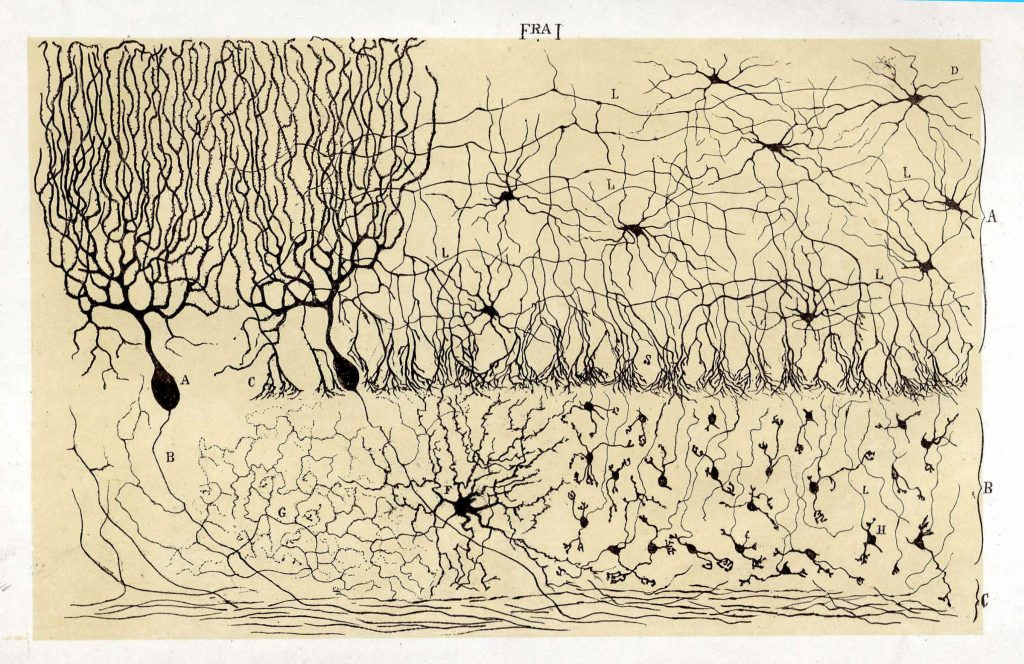
\includegraphics[width=\textwidth]{img/intro/CajalCerebellum.jpeg}
    % https://es.wikipedia.org/wiki/Doctrina_de_la_neurona#/media/Archivo:CajalCerebellum.jpg
    % https://microbioblog.es/la-fascinante-historia-de-la-reazione-nera
    \caption{Representation of cerebellar neurons by Ramon y Cajal.}
    \label{cajal-neuron}
\end{figure}

%From that starting point there have been important findings in the neurons types and structures, such as Glia cells \ref{}. 

The brain is a complex system that we can study from many different prisms. In this thesis, we follow a bottom-up approach. So we will analyze experimentally and theoretically the neural activity at ionic channels and small circuits (with few synapses). Moreover, we will follow a Neurocomputational perspective based on hierarchical sequential information processing, which will be defined in detail in subsection \ref{sec:computational neuroscience}. In the following lines we will approach the basis of neural activation from a computational perspective necessary for the reading flow of this document. We will focus not in their molecular properties but in the change of voltage that they are able to produce and how that inter-operates to give rise to neural activity. 

\subsection{Neuronal dynamics}
Neurons are cells morphologically composed by dendrites, where the connections from other neurons are received through synapses), a soma or cellular body (where information in typically integrated) and an axon (where the information is conveyed as output). Since neurons are the cells that present the largest diversity in morphology, this description does not apply to all neuronal types but serves to start highlighting the importance of spatial scales in the nervous system. 

% As said there are many different ways to study neural dynamics, but a common descriptor for neural activity are action potentials. Action potentials are the 
Neuronal electrical activity is often described in terms of the evolution of membrane voltage caused by the flow of ionic channels between the inside and outside of the cell \parencite{kandel_principles_2012}. The characteristic fast change in the membrane voltage when a neuron fires an output signal is called an action potential or a spike. They are often seen as the minimal pieces of information for reception, processing and transmission carried out by neurons. A more concrete definition of spike could be "an abrupt and transient change of membrane voltage that propagates to other neurons via a long protrusion called an axon" \parencite{izhikevich_dynamical_2007}. Thus, when no inputs are received, the membrane potential of a neuron is negative and it is called resting potential. When this potential is altered by an input that makes the voltage increase, it is known as depolarization. After reaching a peak of voltage, typically a positive value of around 40mV, the potential starts decreasing again. When the potential is more negative than the resting potential, it is known as hyperpolarization. Figure \ref{fig:action potential} illustrates the sequential phases of the action potential generation. 

\begin{figure}[htb!]
    \centering
    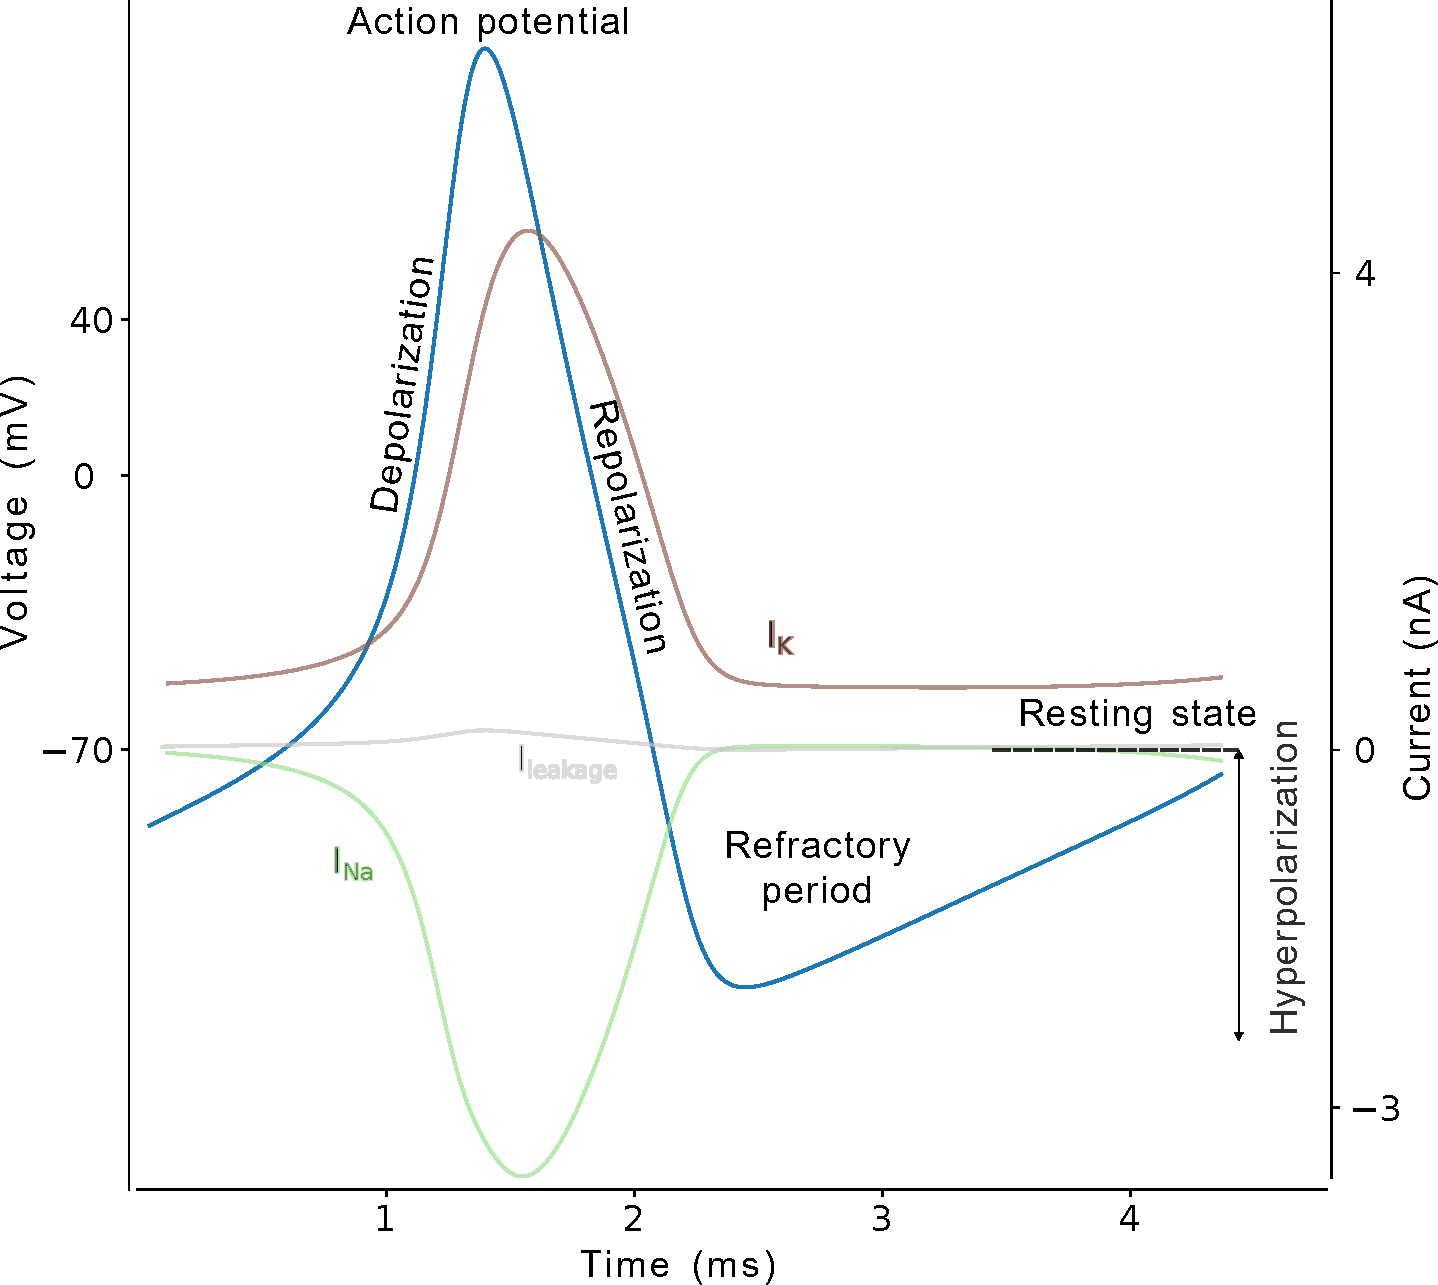
\includegraphics[width=0.8\textwidth]{img/intro/action_potential.pdf}
    \caption{Representation of the sequential  phases and terminology of an action potential. (Adapted from Chris73, Wikimedia Commons, \href{https://creativecommons.org/licenses/by-sa/3.0/}{CC BY-SA 3.0}). In each of this phases of the action potential generation, different ionic channels are activated sequentially, e.g. the sodium channel is involved during the depolarization phase and its activity decais as the potassium channel activates mostly in the repolarization phase. }
    \label{fig:action potential}
\end{figure}

The neural activity is generated by the flow of different ionic channels that counterbalance the voltage value generating the action potential \parencite{koch_biophysics_1999}. The membrane can be composed by different ionic channels, and their dynamics are conditioned by that combination and the possible synaptic connections. These changes in dynamics can be manifested in different ways, but the most notorious ones are the shape and temporal evolution of the action potential. %p61 The Neuron 
For example, in Fig. \ref{fig:spike-types} there is an example of two distinct action potentials with visible differences in their shape, one of them presents a symmetrical shape, where depolarization and repolarization slopes are similar, whereas in the right waveform, there is a notable shoulder in the repolarization and its timescale is almost double in comparison of the example shown in (a).

\begin{figure}[htb!]
    \centering
    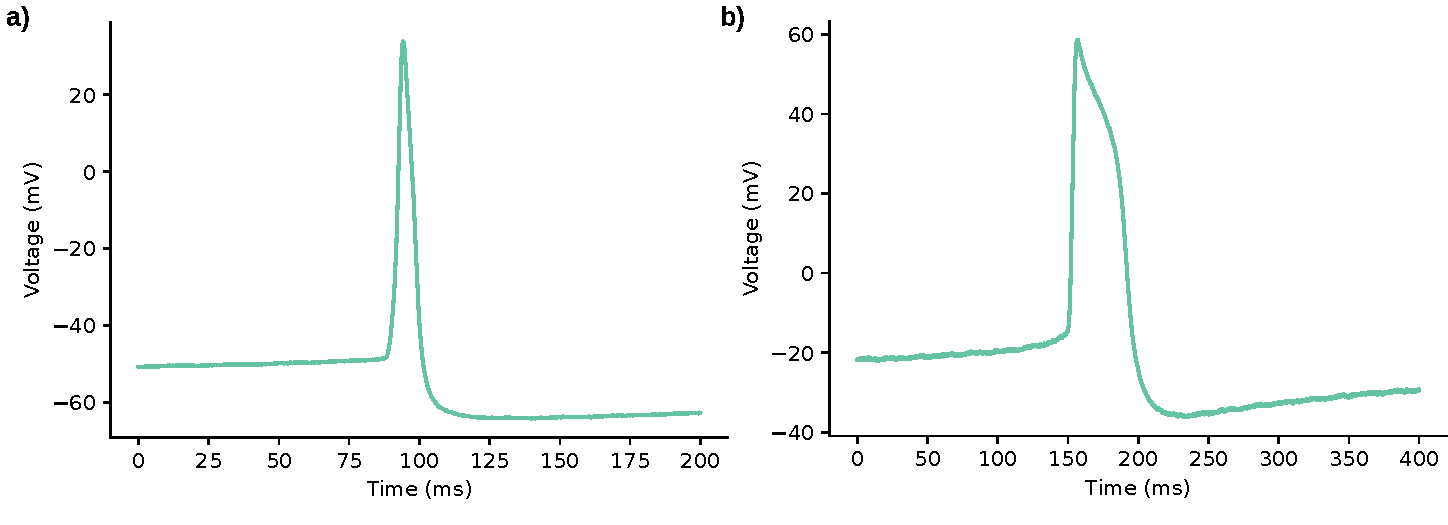
\includegraphics[width=\linewidth]{img/intro/spike-types.pdf}
    \caption{Examples of different spike shapes. Representation of two recordings from two different cells in the right parietal ganglion of \textit{Lymnaea stagnalis}. Left: symmetrical spike; right: shoulder shaped spike.}
    \label{fig:spike-types}
\end{figure}

If spikes are considered minimal pieces of information when coding the neural activity, the combination of these minimal information leads to new forms of information, also known as bursts. Although there is not a fixed description of a burst, and depending on the animal and system a burst might look different \parencite{russell_bursting_1978,palmu_detection_2010,lundqvist_gamma_2016}, there are some common features in bursts: they typically consists of a group of spikes(more than two) on top of a sustained depolarization, and these groups are separated by a hyperpolarization quiescent period called inter-burst interval (IBI). Figure \ref{fig:spike_activity-types} shows several examples of distinct neuronal activities observed in intracellular recordings. Depending on the specific neuron and the circuit, neurons can present tonic firing (first column), at different rates, or bursting activity (second column). 
\begin{figure}[htb!]
    \centering
    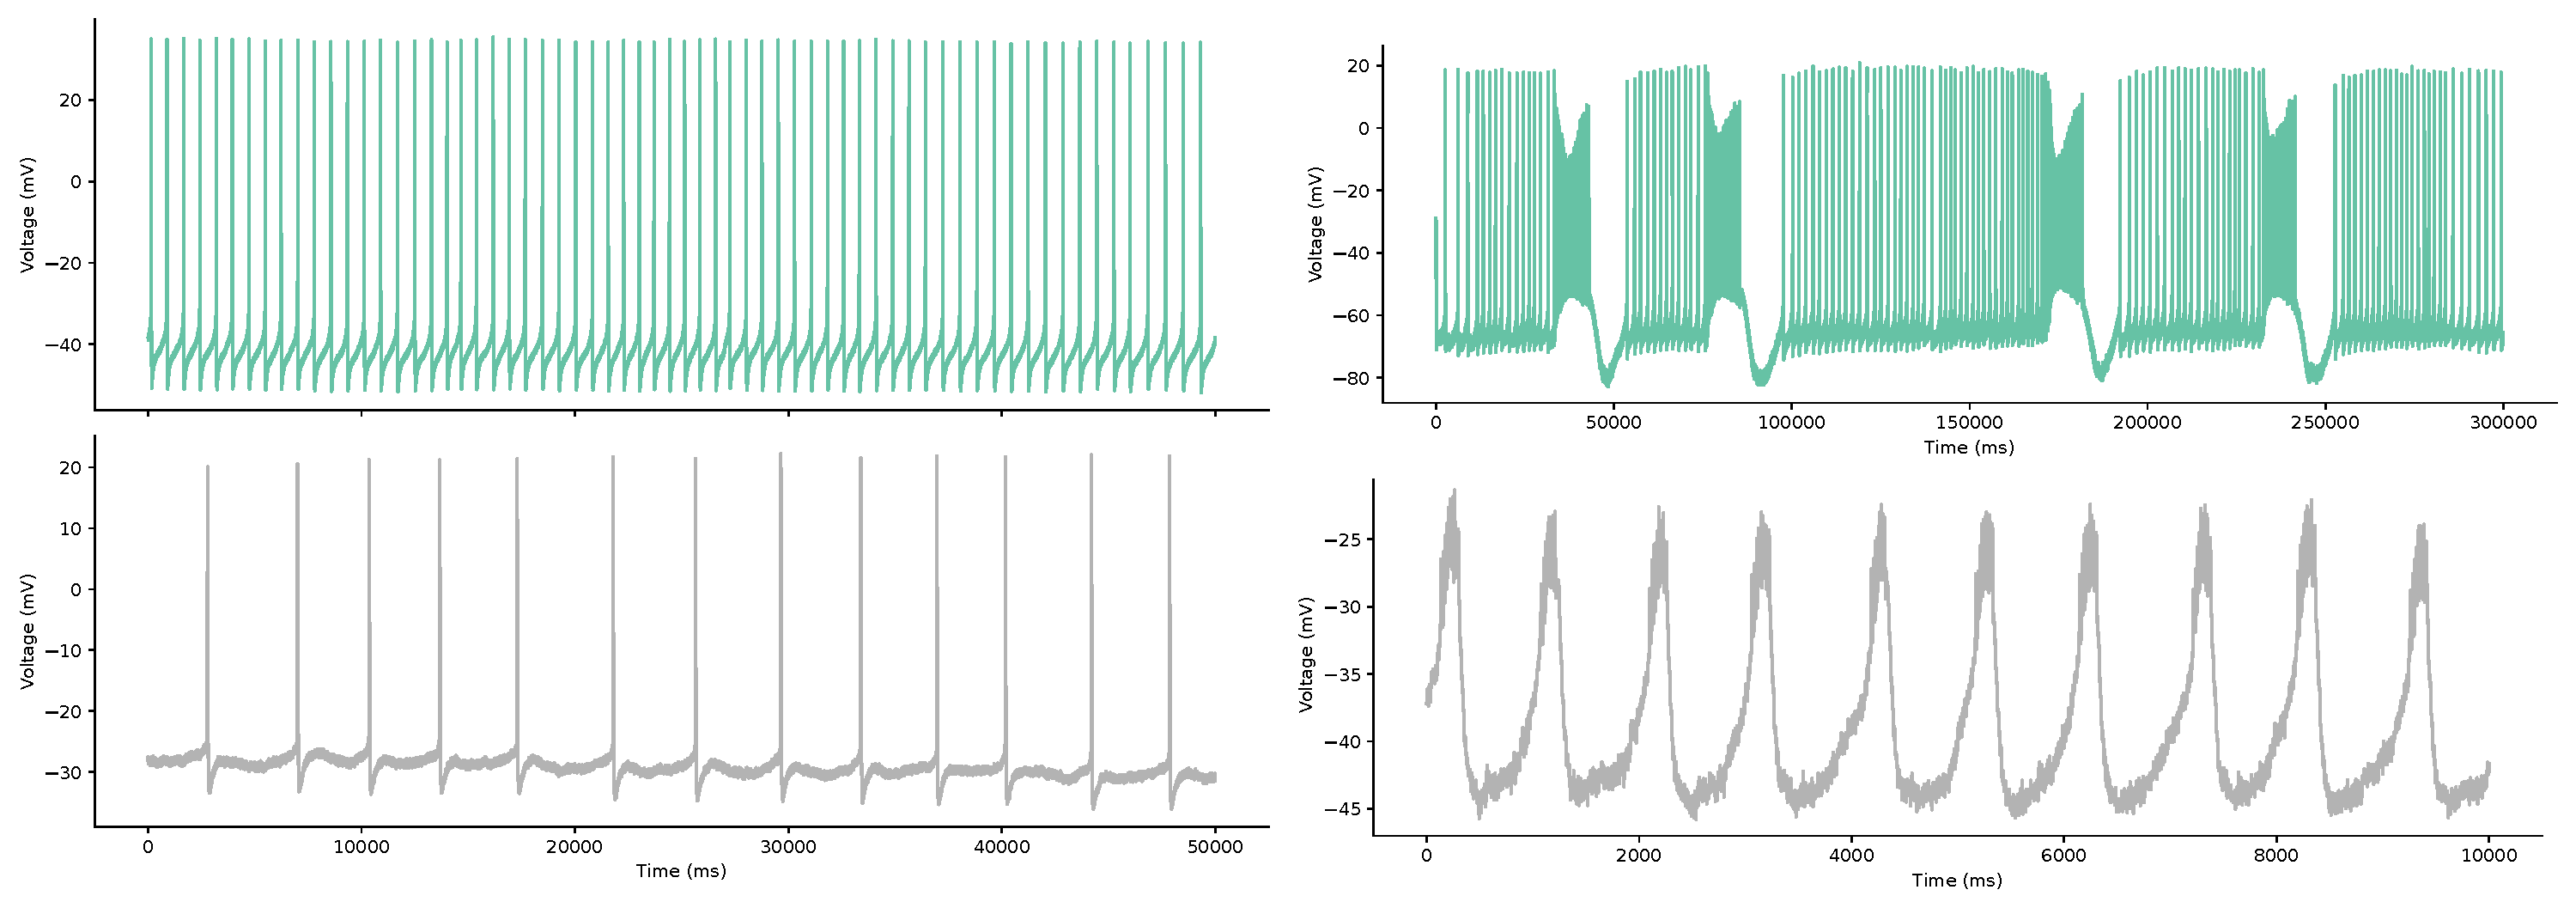
\includegraphics[width=\linewidth]{img/intro/spike_activity-types.pdf}
    \caption{Representation of two examples of different spiking neuronal activity. Left: two simultaneous intracellular recordings in \textit{Lymnaea stagnalis} showing tonic firing at two different frequencies. Right: Two examples of bursting activity, from \textit{Lymnaea stagnalis} (top panel) and from \textit{Carcinus maenas (bottom panel).}}
    \label{fig:spike_activity-types}
\end{figure}

Traditionally, neural codes have been studied focusing on the single spike activation, e.g., by the binarization of the activity (the neuron generates a spike or it does not). Burst can also be informative in terms of the neural activity, either as a whole piece of information or as a complex box of data itself: "bursts are a family of firing patterns that trigger physiological mechanisms not engaged by the same number of spikes in relative isolation" \parencite{friedenberger_silences_2023}. Bursts can be originated either by internal activation, mostly by calcium channels or by the synaptic dynamics involving the corresponding cell (inhibition/excitation) (for an extended review see \parencite{friedenberger_silences_2023}). This is the case in many Central Pattern Generators (CPGs) \parencite{Katz,steuer_central_2018}, which will be discussed in detail bellow and in Chapter \ref{c-invariants-model}.

\subsection{Network dynamics}

Although analyzing the activity of a single neuron is important in terms of characterizing its dynamics, when talking about information processing and behavior, it is also crucial to study the overall circuit dynamics. A circuit of neurons is defined by nervous cells interconnected by synapses. There are two main types of synapses in the nervous system: electrical and chemical connections, see Fig. \ref{fig:synapse-types}. The main difference between them relies on how the communication takes place. Chemical synapses occur through the mediation of \textit{neurotransmitters}, where a presynaptic neuron liberates these molecules that are bound to neuroreceptors to produce an alteration in the postsynaptic neuron. Thus, this connection is asymmetrical and unidirectional, whereas in electrical synapses we find a symmetrical and bidirectional connection. In those synapses, the neurons are almost attached by a structure called \textit{gap junction}, which "pipes" both neurons, in a tissued structure that constrains the leakage to the extracellular space. This communication allows electric charge to flow from one neuron to the other and is then faster than the chemical synapses, which in comparison has no delay. The activity of neurons electrically coupled is usually synchronous \parencite{levitan_neuron_2002}.

\begin{figure}[hbt!]
    \centering
    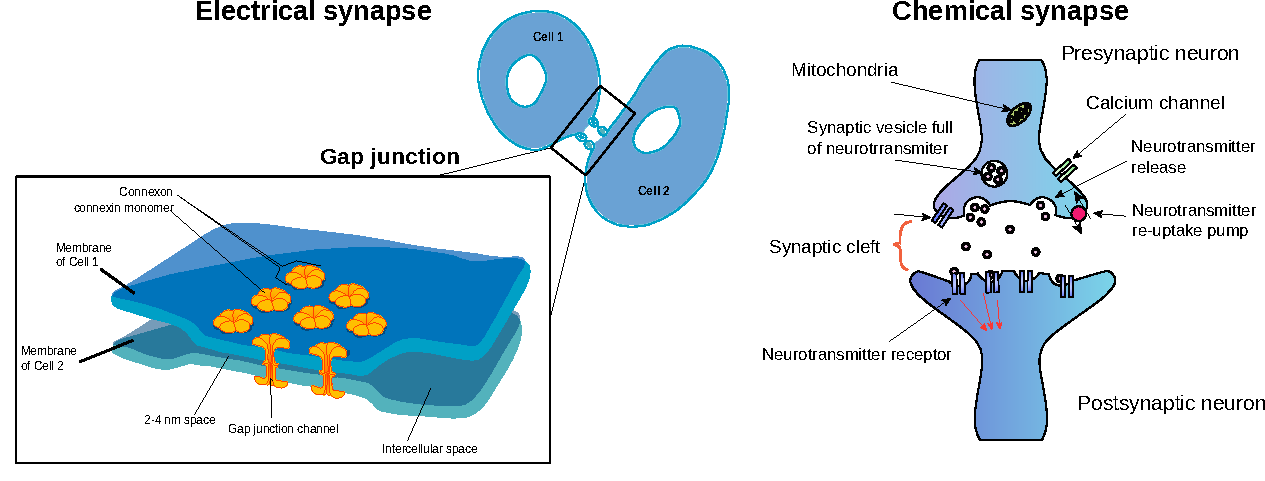
\includegraphics[width=\linewidth]{img/intro/synapses.pdf}
    \caption{Representation of synapses types. Left. Example of electrical synapse between two cells and diagram of gap junction (Adapted from \href{https://commons.wikimedia.org/wiki/File:Gap_cell_junction-en.svg}{Wikimedia Commons}). Right. Example of chemical synapse structure (Adapted from \href{https://commons.wikimedia.org/wiki/File:Synapse_diag1.svg}{Wikimedia Commons})}
    \label{fig:synapse-types}
\end{figure}

In neural circuits, cells  can be connected by one or both types of chemical and electrical synapses, and they usually are also connected to other circuits or modulatory neurons. In Figure \ref{fig:neural circuits} illustrates two examples of circuits at the cellular and macroscopic levels. In this context, there are formed complex system of networks of networks, that might work at different time scales and can take part in one or several functionalities. This interconnection of networks and, from a lower level, cells, leads to sequential activations and transfers of actions into sequences of sequences.

%% Se puede comentar que todas las redes en un circuito neuronal forman parte de otras redes como subcircuitos, que en muchos casos son multifuncionales y que redes de redes generan secuencias de secuencias en lo que se refiere a neural activations

\begin{figure}[hbt!]
    \centering
    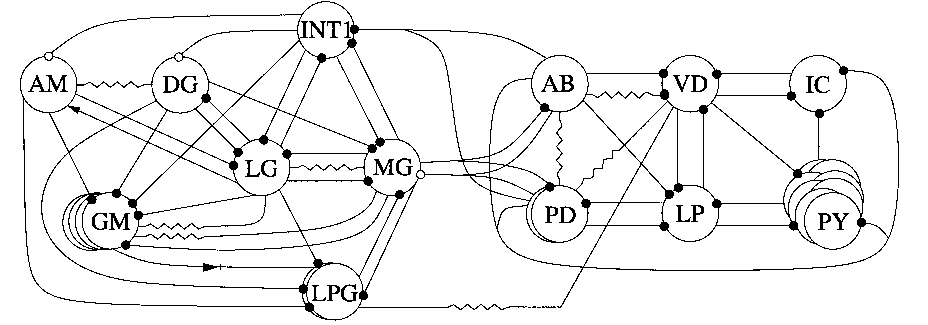
\includegraphics[width=0.64\textwidth]{img/intro/cpg diagram.png}
    \includegraphics[width=0.35\textwidth]{img/intro/The_Human_Connectome.png}
    \caption{Left. gastric and pyloric circuit scheme of \textit{Carcinus Maenas} \parencite{huerta_topology_2001}. Right. Conectome in human brain rendered from 20 subjects (By Andreashorn - Own work,\href{https://commons.wikimedia.org/w/index.php?curid=41581320}{CC BY-SA 4.0})}
    \label{fig:neural circuits}
\end{figure}

\section{The sequential nature of neural dynamics}
%the complex landscape of unanswered questions in the field of neuroscience, from a bottom-up approach.
Brain dynamics can be described as sequences of interactions, from molecules, to neurons, to motor movement and behavior, within a coordinated hierarchy of temporal and spatial scales \parencite{kiebel_hierarchy_2008,yuste05,rabinovich_discrete_2018,Rabinovich23},  from ionic channel activations to sensory encoding, processing, and decision making. Its study reveals fundamental aspects of brain function and cognition, e.g., impulse transmission, executive function, spatial processing or memory.

% There are many important cognitive processes that rely in sequential processes such as perception, memory, decision making, attention and emotion. %Binding \parencite{Michel and coegin 2018, Ravinovich 2020, He 2018}.
% Sequentiallity involves complex pieces of dynamical activity, that when incapsulated as units, can be seen as a chain of events with sequential behaviour \parencite{Ravinovich,2023}.


% Sequential activvation for unsuppervised learning/activity.

%Principles of Brain Dynamics: Global State Interaction Book
%https://www.frontiersin.org/articles/10.3389/fnsys.2014.00219/full
%https://www.ncbi.nlm.nih.gov/pmc/articles/PMC8367843/


%Kiebel 2009
%"Dynamic sequences are generated on various time-scales"
%"Brain is a recognition system that uses an internal model of its environment"

%Kiebel 2008
%"Many aspects of brain function can be understood in terms of a hierarchy of temporal scales at which representations of the environment evolve"


 A common example of sequential  processing is speech, where sequential patterns are present in the structure of phrases, as a sequences of sequences of syllables, words and silences \parencite{kiebel_recognizing_2009}. In this line, an extended case of study is the birdsong, which has  similarity to human's speech, as they involve sequences of coordinated sounds \parencite{prather_brains_2017,fishbein_sound_2019}. Beyond speech, sequential processing is also present in motor movement, from muscle activation to repetitive coordinated actions such as rhythmic tapping or music performance \parencite{ding_temporal_2017}. Also, there are many important cognitive processes that rely in sequential mechanisms such as perception, memory, decision making, attention and emotion \parencite{Varona2016, he_robust_2018, rabinovich_sequential_2020}.

However, it is not clear how exactly the brain processes time. In contrast to the theory of a central clock that manages time for every behavioral task, the theory of a distributed time processing \parencite{buonomano_temporal_1995,ivry_representation_1996} is well accepted. In this framework, especially in movement coordination, there is a need for circuits that manage the sequential rhythmic activity. This is the case of Central Pattern Generators (CPGs), circuits of neurons with closed-topology that sequentially activate neurons and generate coordinated motor activity \parencite{selverston_reliable_2000}. They are present in many systems, from insects to humans \parencite{pearson_central_1972,marder_central_2001,mackay-lyons_central_2002,minassian_human_2017}. There are several key aspects that make these circuits an interesting case of study. First, their neurons are organized in closed-topologies receiving all feedback from companion cells \parencite{huerta_topology_2001}. These circuits are able to maintain a rhythmic activity in an autonomous manner, typically by mutual inhibitory interactions~\parencite{katz_evolution_nodate}. Second, their activity is flexible enough to adapt to changes in the context, e.g., variations in the terrain while walking. Finally, they are present in many systems and in some of them there is a direct relationship between the activity of the neurons in the circuit and the motor movement that they produce. For example, in the stomatogastric CPG in the crab \textit{C. maenas}, in charge of the pylorus movement, the PD (pyloric dilator), LP (Lateral Pyloric) and PY (PYloric) neurons correspond to the pylorus dilatation, pylorus close and contraction of the rostral constrictor to move food in the digestive system \parencite{moulins_introduction_1987,selverston_oscillations_2006}.

\begin{figure}[hbt!]
	\centering
	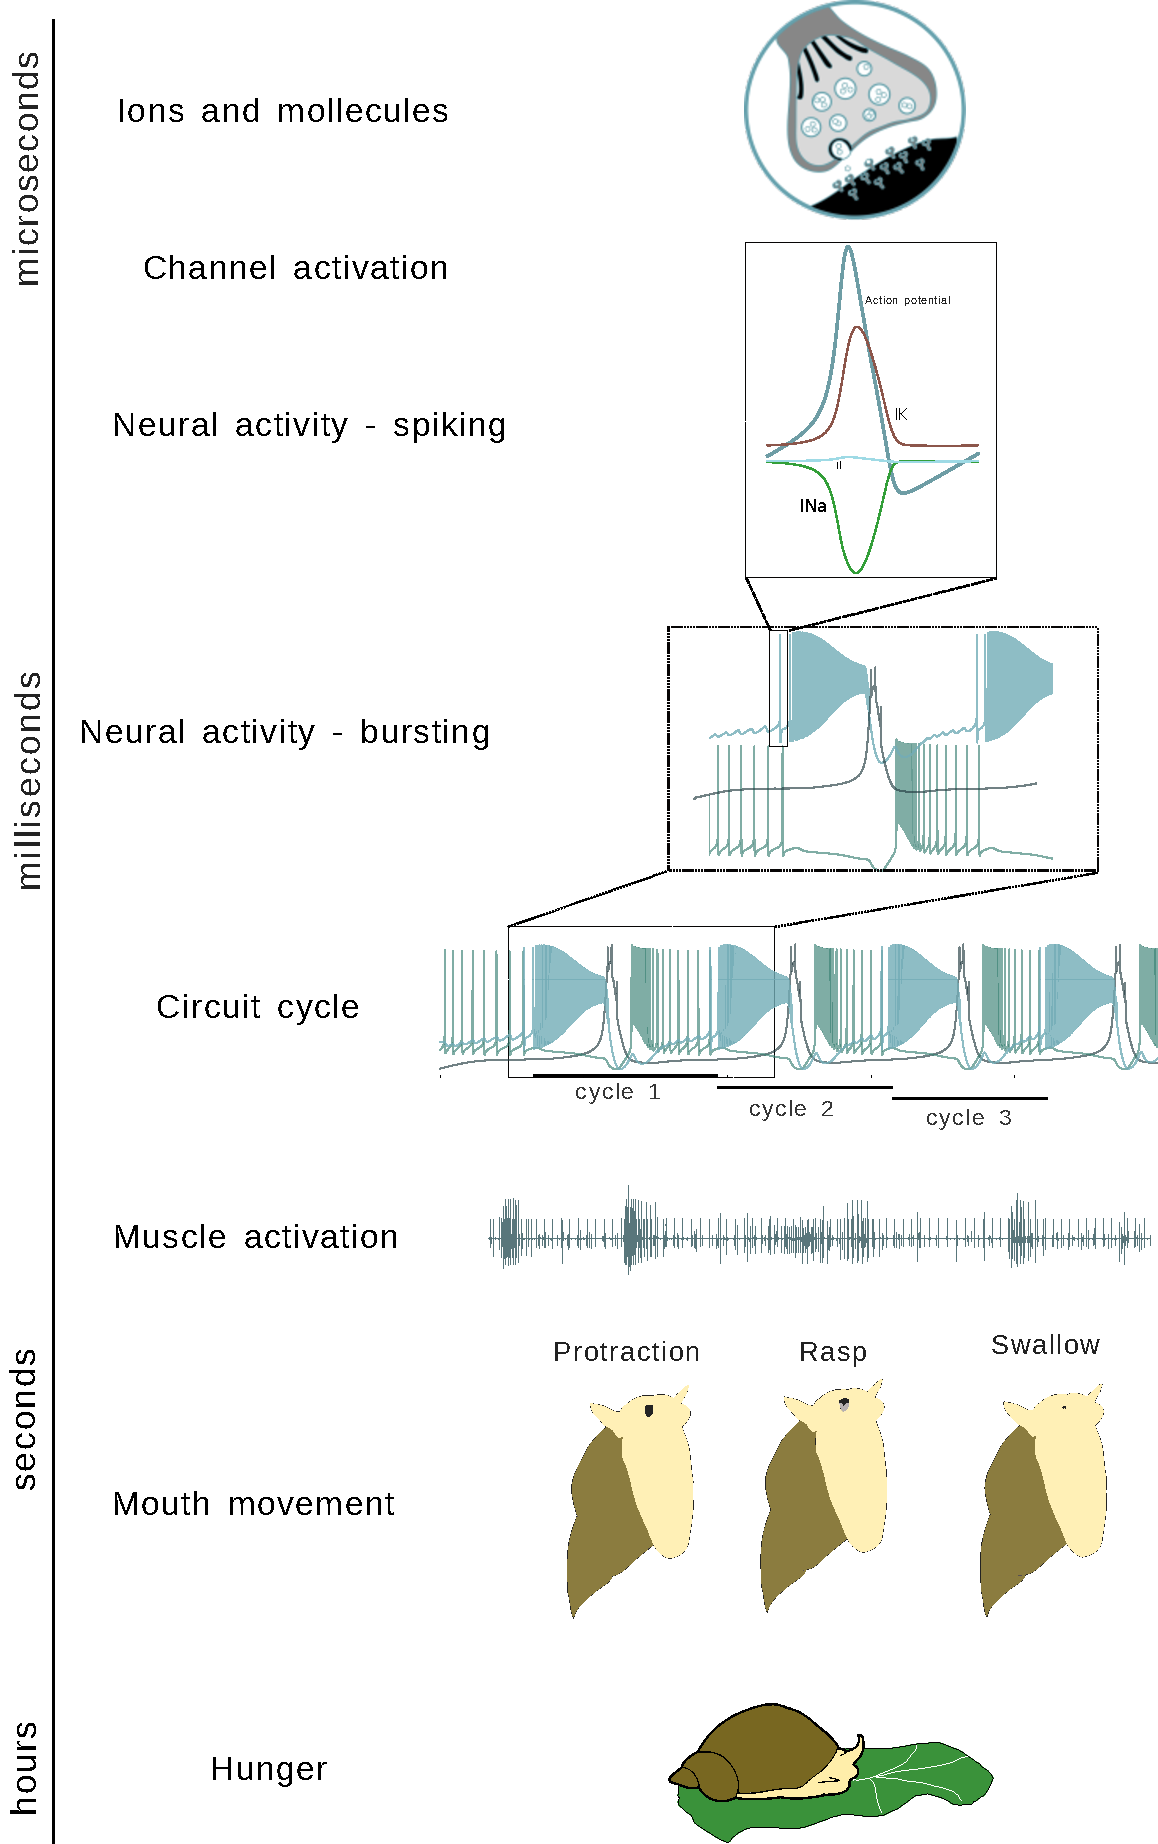
\includegraphics[width=0.9\textwidth]{img/intro/time scale/time-scale-feeding.pdf}
	\caption{Illustration of the sequential feeding process at different time scales in {\sl Lymnaea stagnalis}.}
	\label{fig:time scale feeding}
\end{figure}

The sequential activity in the brain goes from the sub-millisecond scale to days (the time scale of circadian rhythms \parencite{mauk_neural_2004}). Figure \ref{fig:time scale feeding} shows an illustrative example of the sequential nature of neural activity at different scales in the generation of coordinated motor activity in the feeding of a snail. At the scale sub-milliseconds, there is a flow of ions that generate a sequence of ionic channel activation, that in the scale of milliseconds produce action potentials. The combination of them in form of rhythmic bursts, activate the corresponding muscles at the scale of seconds and generate the necessary sequential movement to eat: open the mouth, rasp food and swallow, that is  repeated along the day. 


The study of the action potential dynamics and the interaction between ionic channels and synapses is crucial, since it is a key part in any brain process, and it cannot be detached from the whole. The alteration of the dynamics of these channels at different sites along the neuron can affect synaptic inputs/outputs, how the neurons communicate and the resulting process. Ionic channels are the starting point of the electrical signals underlying neuronal network activity, and their malfunction can contribute to neural disorders \parencite{kecskes_editorial_2023}. Thus, understanding brain activity not only at large scales but also from the stage of voltage generation dynamics can be crucial for a real and complete understanding of neural systems. Their study can also help distinguish between short- and long-term modulation, a key aspect in neural plasticity and the application of neuromodulatory techniques \parencite{chambers_light-activated_2008,burke_modulation_2019}.

%Regarding sequential studies, it is common to talk about neural activity as blocks of information and as a binary on-off event, even for whole brain areas, classifying tasks by those findings. Although the findings under this approach have been undoubtedly relevant, they usually do not consider the importance of dynamics, variability and how their processing affects behavior.
 
%Although often disregarded in macroscopic studies and as a consequence in bottom-up approaches,
It is important to explore the mechanisms that allow to maintain a robust sequential activity despite changes in context and the variability underlying the neural dynamics. Action potentials and bursts can be classified depending on their waveform shape and grouped spiking activity. However, in those subgroups there is a high intra-variability, where for example bursting activity can differ in shape and duration, i.e., number of spikes in a bursts. Figure \ref{fig:burst variability} shows an example of the variability in the burst waveform and duration for a sequence of several bursts. 


\begin{figure}[htb!]
	\centering
	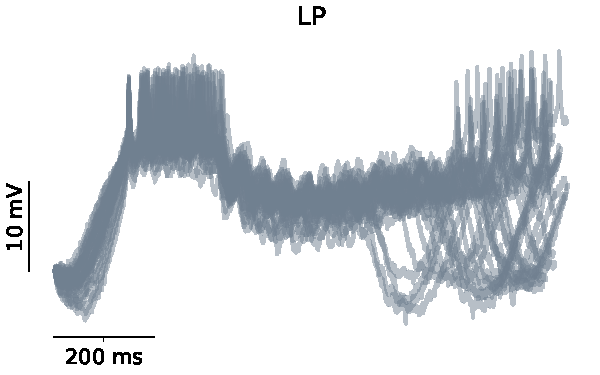
\includegraphics[width=0.6\textwidth]{img/intro/burst_variability.pdf}
	\caption{Superimposition of bursts at different time instants aligned by the first spike in the burst for intracellular recordings of an LP neuron in the sthomatogastric CPG.}
	\label{fig:burst variability}
\end{figure}

The study of this variability unveils key factors in the sequentiallity and how it is maintained despite different intrinsic or external modulations. This is the case for example of sequential dynamical invariants, i.e., robust relationships between time intervals that conform a neural sequence, when analyzing the activity cycle-by-cycle \parencite{reyes_artificial_2008,elices_robust_2019,garrido-pena_characterization_2021,berbel_emergence_2024}. This sequential dynamical invariants might have a crucial role understanding the coordination of sequential activity and the balance between robustness and flexibility required for effective function in many brain processes \parencite{tatsuno_analysis_2015,ullen_neural_2003,zimnik_independent_2021,zhou_neural_2020,dragoi_cell_2020}. We will discuss in detail this phenomena in the feeding CPG of \textit{Lymnaea stagnalis} in chapter \ref{c-invariants}.


\section{Studying neural dynamics in computational models.}
\label{sec:computational neuroscience}
Computational Neuroscience is a subfield of neuroscience that uses theoretical and computational techniques to address the study of nervous system at multiple levels, from the molecular level all the way to the complex networks that shape behavior. It is thus a multi-disciplinary field. The basis of Computational Neuroscience lay on the understanding of brain dynamics from its electrical signals and the information they carry \parencite{schwiening_brief_2012,catterall_hodgkin-huxley_2012,dimitrov_information_2011,shannon_mathematical_1948}. Computational Neuroscience has extended its scope, leading to new paths of research including complex networks, graph theory, single cell analysis and machine learning techniques \parencite{cns2023}. In fields such as Artificial Intelligence there is even a symbiotic relationship between fields, where both inspire and help each other grow \parencite{amunts_human_2019,wozniak_deep_2020,goncalves_training_2020}.

An important part of Computational Neuroscience is the description of neural systems with theoretical models and the reproduction of key phenomena by the model simulation. The simulation of neural activity is a powerful tool to explore neuronal dynamics, its biophysical sources, the possible mechanisms underlying the neural signaling, and the observed complex information processing. Its strength relies on the complete accessibility to the variables of the model, the typical extensive range of tunable parameters in the model which can be explored,  and the ability to assess the role  of distinct elements in the system or circuit by including or excluding them in the simulations. Although models cannot fully substitute research on living systems, they do lead us closer to the understanding of complex neural dynamics, being a fast, effective and a low cost alternative to advances in science.  Also, models are an essential complement to experimental neuroscience reaching detailed descriptions where experimental approaches such as electrophysiology have limitations arising from the always present partial observability. 
%Like science is not about truth, but about knowledge, models do not aim to substitute living systems, but to lead us closer to the insight of neural dynamics. %#ToDo revisar

Models can be classified by their level of description, i.e. what level of simplification/abstraction is used, the detail of the structure/phenomenon being modeled and the size of the network, or their ability to reproduce the observed neural activity, e.g. chaotic dynamics. Figure \ref{fig:models-classification} illustrates such kind of classification, with examples of models of large networks as \cite{potjans_cell-type_2014,bezaire_interneuronal_2016}, of single cell but still detailed as in \cite{smith_dendritic_2013} and more abstract descriptions such as the one proposed in \cite{izhikevich_simple_2003}. Regarding the level of description, in the different biophysical models there is always a choice between detailed description of non-linearities, channels and excitation properties, and efficiency in computation. In this line, researches can choose from conductance-based models  \cite{hodgkin_quantitative_1952}, rich in the description of nonlinearities or simplified dynamical models  \cite{hindmarsh_model_1984,fitzhugh_impulses_1961}, which typically represent nonlinearities with polinomial simplifications (see \cite{torres_modeling_2012} for a review of different levels of neuronal modeling. 


%Adapt models table from
%https://www.sciencedirect.com/science/article/pii/S0896627319304441 Figure 2A:
\begin{figure}[bth!]
	\centering
	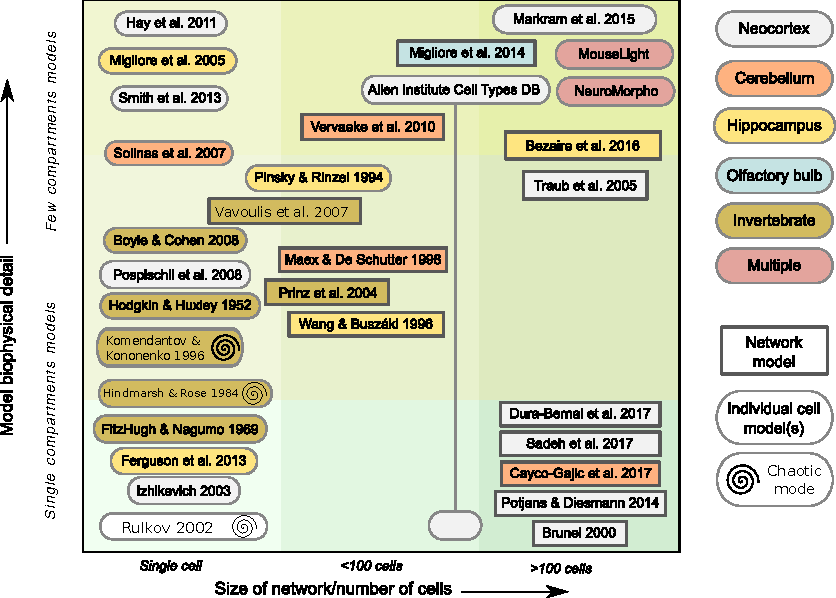
\includegraphics[width=\textwidth]{img/intro/models classification_v2.pdf}
	\caption{Neural and network models classified by biophysical detail, structure modeled and size of the network. Figure adapted from Fig. 2 \cite{gleeson_open_2019} under \href{http://creativecommons.org/licenses/by/4.0/}{Creative Commons CC-BY license}. Models are classified by the biophysical detail, by y-axes being the models in the bottom the less specific ones; by the size of the network modeled, from left to right one cell to hundreds of cells; and by the brain-structure they model, represented in colored boxes. The shape of the box also classifies the model in network model or individual cell model. A third category was here included from the original work, representing by an spiral in the box the ability of the model to produce chaotic activity without external alterations, i.e, reproduce spontaneous variability. Although the figure does not contain all model approaches, it illustrates key milestones in neuronal modeling. }
	\label{fig:models-classification}
\end{figure}
\subsection{Conductance-based models}

In this thesis, all experimental recordings have been supported with simulations on conductance-based models. They are defined as mathematical descriptions of the ionic channels dynamics, based on their voltage-dependent conductance. The pioneer study by \cite{hodgkin_quantitative_1952} defined dynamical equations based on the equivalent electrical circuit of the electrical properties of neurons in \textit{Aplysia}, see Fig.  \ref{fig:electrical circuit}. This modeled circuit is also used to conform the intracellular recording configuration, where the pipette is included as an extra current compensated by the electrode in the bath (see Fig. \ref{fig:clamp circuit}).

\begin{figure}[htb!]
	\centering
	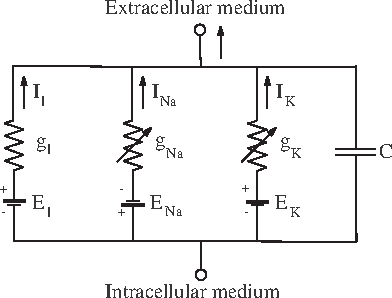
\includegraphics[width=0.7\textwidth]{./img/intro/electrical_circuit.pdf}
	\caption{Electrical circuit describing the membrane voltage in a conducatance based neuron model.}
	\label{fig:electrical circuit}
\end{figure}

\begin{figure}[htb!]
	\centering
	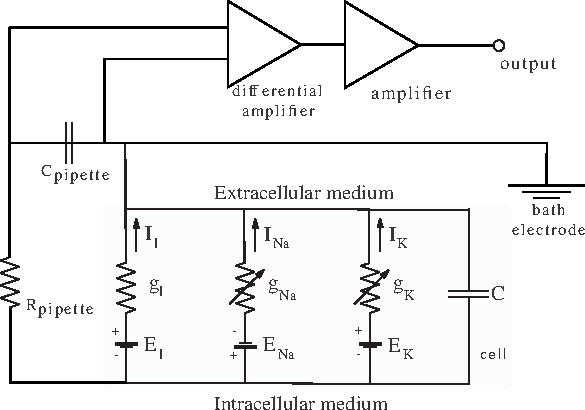
\includegraphics[width=0.7\textwidth]{./img/intro/intracellular_recording_circuit.pdf}
	\caption{Electrical circuit representing the scheme for intracellular recordings.}
	\label{fig:clamp circuit}
\end{figure}


In these models, the simulation of neural electrical activity is based on the mathematical description of different ionic channels in the circuit, whose dynamics are also well defined by activation gates. First, there is a mathematical description of the voltage dependency on time, as described by the equation \ref{eq:voltage ions}:

\begin{equation}
 C_m \frac{dV}{dt} = I - \sum I_{x},
  \label{eq:voltage ions}:
\end{equation}

where $V$ is the membrane potential, $I$ is an external current, e.g. an external stimulus or a synaptic current, $I_{x}$ is the current description for each channel involved in the action potential generation, e.g., sodium, potassium, calcium ( $I_K$, $I_{Na}$, $I_{Ca})$.

Second, each channel is also described voltage-dependent composed by activation-gates dynamics:
\begin{equation}
I_x =  g_x m^n h^n (V - E_x), 
\end{equation}

where $g_x$ is the corresponding conductance of the channel, $E_x$ is the reversal potential for that channel and $m$ and $h$ represent activation and inactivation variables, respectively.
Activation gates usually have an exponential tendency, and are defined by activation and inactivation dynamics, also dependent on voltage and time. They follow the structure in equation \ref{eq:alpha-beta}

\begin{equation}
	\label{eq:alpha-beta}
	\frac{dm}{dt} = \frac{m_{\infty,i}-m_i}{\tau_{m,i}}
\end{equation}

where $\tau_{m,i}$ are the relaxation time constants which are usually voltage-dependent and modeled using sigmoid or Gaussian functions. Note that $m$ was used here but this formula corresponds also to inactivation variables. 


Following the Hodgkin and Huxley formalism, 
the equations that describe the voltage dynamics and the conductance dynamics of the active channels (Na and K) in the circuit shown in Fig. \ref{fig:electrical circuit} are:
%\begin{equation}
%		C \frac{dV}{dt} = I - g_K n^4 (V - E_K) - g_{Na} m^3h(V-E_{Na}) - g_L (V-E_L)
%\end{equation}

% Please add the following required packages to your document preamble:
% \usepackage{multirow}
\begin{table}[h!]
	\begin{tabular}{lccc}
		Voltage equation                                                                 & \multicolumn{3}{c}{$C \frac{dV}{dt} = I - g_K n^4 (V - E_K) - g_{Na} m^3h(V-E_{Na}) - g_L (V-E_L)$}                                                                                                                                  \\ \hline
		& \multicolumn{2}{c}{Activation variables}                                                                                                                              & Inactivation variable                                        \\ \hline
		\multicolumn{1}{c|}{\begin{tabular}[c]{@{}c@{}}gating \\ variables\end{tabular}} & \multicolumn{1}{c|}{$\frac{dm(t)}{dt}=\frac{m_{\infty}(V(t))-m(t)}{\tau_m(V(t))}$} & \multicolumn{1}{c|}{$\frac{dn(t)}{dt}=\frac{n_{\infty}(V(t))-n(t)}{\tau_n(V(t))}$} & $\frac{dh(t)}{dt}=\frac{h_{\infty}(V(t))-h(t)}{\tau_h(V(t))}$ \\ \hline
	\end{tabular}
%	\begin{tabular}{cccc}
%		\multicolumn{1}{l}{Voltage equation}                                                              & \multicolumn{3}{c}{$C \frac{dV}{dt} = I - g_K n^4 (V - E_K) - g_{Na} m^3h(V-E_{Na}) - g_L (V-E_L)$}                                                                                                       \\ \hline
%		\multicolumn{1}{l}{}                                                                              & \multicolumn{2}{c}{Activation variables}                                                                                                                 & Inactivation variable                          \\ \hline
%		\multicolumn{1}{c|}{\begin{tabular}[c]{@{}c@{}}gating \\ variables\end{tabular}}                  & \multicolumn{1}{c|}{$n = \alpha_n (V)(1-n)-\beta_n(V)n$}                    & \multicolumn{1}{c|}{$m = \alpha_m (V)(1-m)-\beta_m(V)m$}                   & $h = \alpha_h (V)(1-h)-\beta_h(V)h$            \\ \hline
%		\multicolumn{1}{c|}{\multirow{2}{*}{\begin{tabular}[c]{@{}c@{}}transition \\ rates\end{tabular}}} & \multicolumn{1}{c|}{$\alpha_n(V)=0.01\frac{10-V}{\exp(\frac{10-V}{10})-1}$} & \multicolumn{1}{c|}{$\alpha_m(V)=0.1\frac{25-V}{\exp(\frac{25-V}{10})-1}$} & $\alpha_h(V)=0.07\exp\frac{-V}{20}$            \\ \cline{2-4} 
%		\multicolumn{1}{c|}{}                                                                             & \multicolumn{1}{c|}{$\beta_n(V)=0.0125\exp(\frac{-V}{80})$}                 & \multicolumn{1}{c|}{$\beta_m(V)=4\exp(\frac{-V}{18})$}                     & $\beta_h(V)=\frac{1}{\exp(\frac{30-V}{10})+1}$ \\ \hline
%	\end{tabular}
	\label{table:hh-equations}
\end{table}

This combination of channels generates the spike waveform shown in Fig. \ref{fig:spike-types model}a) but, as in living systems, the combination of different channels leads to distinct outputs, e.g. shoulder and no-shoulder type neurons (see previous section, Fig. \ref{fig:spike-types}). This is the case of waveform in Fig. \ref{fig:spike-types model} b), where this shoulder shape could be reproduced in models by including calcium specific channels.

\begin{figure}[htb!]
	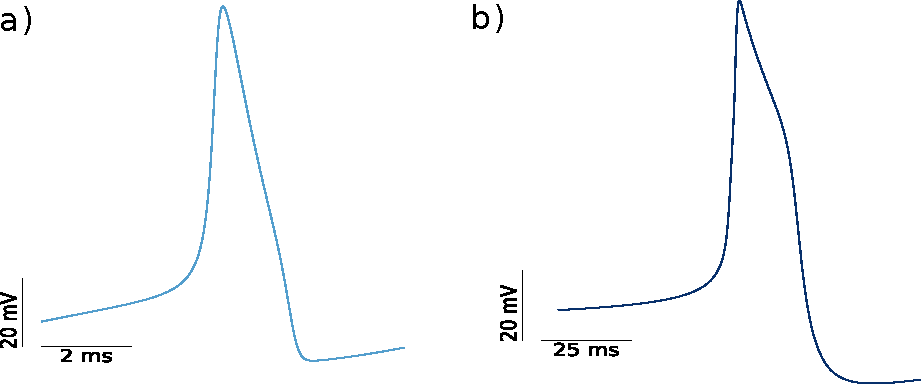
\includegraphics[width=\textwidth]{img/intro/spike-types model.pdf}
	\caption{Simulation of two distinct spike types: no shoulder (a) and shoulder shaped (b), described by equations in \cite{hodgkin_quantitative_1952} and \cite{vavoulis_balanced_2010}, respectively}
	\label{fig:spike-types model}
\end{figure}

\subsubsection{\large{Modeling networks}}
\label{c-intro-synapses}
In addition to the modeling of the action potential generation, synapses can also be modeled with different mathematical representations depending on the type and the level of specificity. Synapses are introduced in conductance-based models as an extra current that simulates the alteration in the neuron dynamics by chemical or electrical synapses. In conductance based models, electrical synapses or gap junctions are usually defined by the following equation:
\begin{equation}
    I_{ij}(t) = \bar{G}_{ij} (V_i(t) - Vj(t))
\end{equation}
\noindent where $i$ and $j$ represent the two neurons conforming the electrical synapse and $\bar{G}_{ij}$ is a constant representing the maximum value of synapse conductance in the connection. For symmetrical gap junctions, the other cells receives exactly the same current with inverse sign.

On the other hand, chemical synapses are by definition asymmetrical and can be described as in equation \ref{eq:synapse binary}:
\begin{equation}
     I_{ij}(t) = G_{ij}(t) (V_i - E_j^{syn})
     \label{eq:synapse binary}
\end{equation}
\noindent where $E_j^{syn}$ is the voltage value at which the synaptic current cancels and $G_{ij}$ can now have complex dynamics considering the trafficking of neurotransmitters as in equation \ref{eq: Gii} \parencite{torres_modeling_2012}. 

\begin{equation}
	G{ij}(t) = \bar{G_{ij}}  \Theta(t-t_j^{sp}) \alpha (t-t_j^{sp})
	\label{eq: Gii}
\end{equation}
\noindent where $\bar{G_{ij}}$ is the constant value for the conductance, ${t_j}^{sp}$ is the time at which the presynaptic spike occurs. $\Theta(x)$ is the Heaviside step function and $\alpha(t)$ is a function to model an evoked postsynaptic responses that can be defined by exponential functions.

Depending on the selection of this level of specification, the neuron can be activated by a (i) binary cause: occurrence or absence of an action potential, or (ii) a dynamic model that is also dependent on the the postsynaptic voltage level (e.g. a graded synapse) or represents phenomena such as synaptic depression or facilitation. In that second case the level of specification is higher, with a richer description of the synapse dynamics. This is the case for example of \cite{tsodyks_neural_1997}, represented in equations \ref{eq:tsodyks1},\ref{eq:tsodyks2} or the gradual synapse in the CPG model by \cite{vavoulis_dynamic_2007}, discussed in methods chapter, section \ref{sec:CPG model}.


\begin{equation}
	\frac{dU}{dt} = -\frac{U}{\tau_{\text{rec}}} + U_{\infty}(1 - U) \delta(t - t_{\text{spike}})
	\label{eq:tsodyks1}
\end{equation}
\begin{equation}
	\frac{dX}{dt} = -\frac{X}{\tau_{\text{fac}}} + (1 - X) \frac{U(t_{\text{spike}})}{U_{\infty}} \delta(t - t_{\text{spike}})
	\label{eq:tsodyks2}
\end{equation}


\subsection{Variability in computational models}

Most studies use deterministic models that produce regular neural activity, which are sufficient for many research questions when exploring input/output responses, studying the role of different biophysical elements or supporting experimental results on steady state dynamics. However, living systems are highly variable, often working in transient regimes, often displaying chaotic activity, and still able to produce sequential and robust patterned activity~\parencite{selverston_reliable_2000}. Variability in the activity of living neurons has been proven to play an important role in relevant information processing tasks. While this is a key aspect in neural dynamics, models usually exclude intrinsic variability from their description,  particularly in membrane potential waveforms and in collective adaptive dynamics. To induce some level of stochasticity, models typically include Gaussian noise as external input \parencite{linaro_accurate_2011,pezo_diffusion_2014,zheng_spontaneous_2020}. However, this is a limited approach when exploring the role of variability intrinsically and dynamically generated by the the neurons and the circuits for a specific computational tasks, e.g. for sequence coordination. There are several possibilities to include variability in neuronal intrinsic dynamics as it is the example of \cite{hindmarsh_model_1984} or \cite{komendantov_deterministic_1996}, where in both descriptions, there is a combination of parameters that lead both to a chaotic state, where the resulting activity is not regular. When the source of the variability in the system comes from its intrinsic properties, there is a possibility to study its dynamics and the role of this variability in the system without random sources, which in cycle-by-cycle dynamics can canceled out.

\section{Vertebrate and invertebrate animal studies}
\label{c-intro-invertebrates}
The study of neural dynamics and behavior is carried out using many different animal models. Apart from the hegemonic rodents models, there have been invaluable findings using invertebrates, such as in genetics and developmental biology in \textit{C. elegans} \parencite{brenner_genetics_1974}, \textit{Zebra fish} \parencite{streisinger_production_1981} and \textit{Drosophila} \parencite{nusslein-volhard_mutations_1980}; neural dynamics in \textit{Aplysia} \parencite{wachtel_direct_1967}, motor activity in \textit{Panulirus} \parencite{SELVERSTON1976} and \textit{Carcinus maenas} \parencite{eisen_mechanisms_1982} or \textit{Lymnaea stagnalis} \parencite{Benjamin1979b}, the main animal model in this thesis. Besides those examples, these animal models have been used for a wide variety of fields including behavioral studies, ecotoxicology, evolution, human disease modeling, etc. \parencite{romanova_animal_2018} 

Despite brain differences between invertebrates and mammals, there are many universal characteristics of nervous systems that can be extrapolated to humans. We should keep in mind that any animal model is still a research framework, with differences from the real focus of study --the human brain-- and as a model, there are differences in the structure, even within mammal species \parencite{preuss_taking_2000}. So by using computational models or exploring more animal species there can be set a better ground truth for the aspects that shape the neuronal and behavioral dynamics. 

 % https://karger.com/bbe/article-abstract/55/6/287/46613/Taking-the-Measure-of-Diversity-Comparative?redirectedFrom=fulltext  
 %First, by examining a wider range of species than are currently employed, and by using modern techniques of phyletic analysis, neuroscientists can more rigorously identify those features of cortical organization that are, in fact, widely shared among mammals or among particular mammalian subgroups. Second, by taking account of variations, neuroscientists can abstract more reliable and general principles of structure-function relationships in the nervous system. Finally, freed from the doctrine of basic uniformity, neuroscientists can pursue the study of human cortical specializations, and so advance our understanding of what distinguishes humans as a biological species.

Findings in invertebrates are sometimes overlooked, often under the excuse that features in invertebrates cannot be extrapolated to humans. However, invertebrates  models  have proven their utility not only in basic science. We can find examples of this in human diseases, memory, motor activity and neuromodulation. Particularly, in the study of neural processes, the ease of accessibility and finite number of large neurons in the system, have made invertebrates an interesting case of study. In Figure \ref{fig:invertebrates timeline} there is a timeline containing key discoveries in Neuroscience, some of them Nobel Prize winners in the last century, as well as current relevant discoveries in the field. 
% https://docs.google.com/spreadsheets/d/16rOG5LSuFMQGHAakeYqcdG26NIZnY4NWtr6TZku_UKs/edit#gid=0

Among the advantages in using invertebrates, it is worth mentioning the easy access to the nervous system, the ease of breeding and reproduction or the simplicity of their biological features, that makes possible a full description of it, i.e. the genomic description of \textit{C. elegans} or the nervous system in \textit{Lymnaea stagnalis}. Also some selected species were a main field of study in the last decades, so there is plenty of literature for each one even in different fields. Furthermore, despite the simplicity of these systems, their nervous system is still capable of generating robust sequential neural activity, preset behavior and even learning processes. 


Apart from the possible advances in science from a productivist view, invertebrates models can also bridge the gap between resources and science, allowing low-income labs and countries to \textit{do} science. This animal models are usually cheaper to obtain, maintain and there is usually a possibility of breeding own colonies. This makes their use extendable and breaks some economical barriers in science, where high-income countries usually centralize the science production with strong conventions \parencite{castillo_spineless_2017,stephan_how_2015}. 

%\textit{What can computational neuroscience provide to experimental approaches}

However, in any animal model is still good to remember that the aim in science and progress should be advances in science but not at all costs. Alternatives such as computational models should be a predefined complement to experimental studies, reducing their necessity and leading to a less harmful alternative to the human's necessity of knowledge. \todo{revisar si quitar}


\subsubsection{\textit{Lymnaea stagnalis}, the great pond snail}
In this thesis, we explore the neural system of the great pond snail, \textit{Lymanea stagnalis}. This mollusk has been an important case of study since the late XX century, when it was used extensively to study neurobiological processes and nervous system functioning. This carreer-time effort lead to a detailed description of the buccal ganglia 
%\begin{wrapfigure}{l}{0.3\textwidth}
%	\centering
%	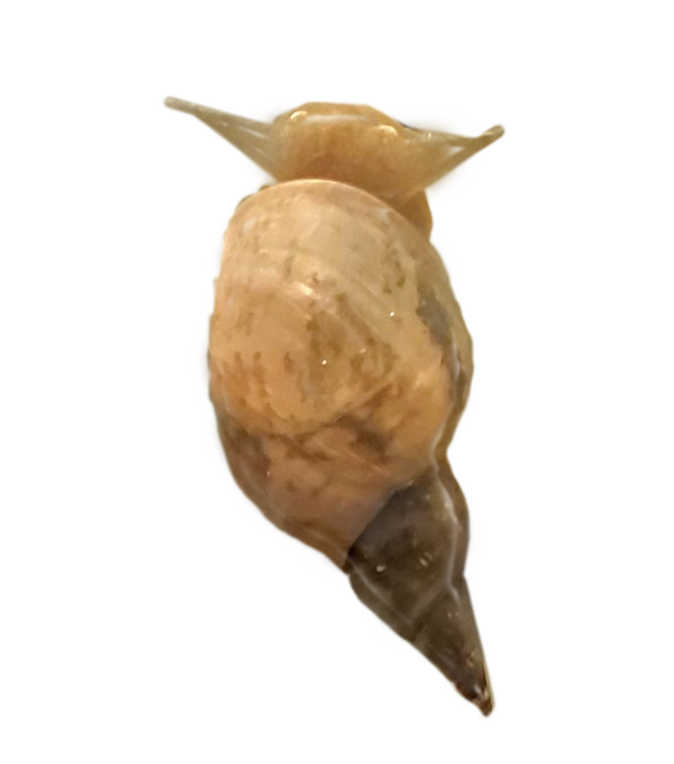
\includegraphics[width=0.7\linewidth]{img/intro/lymnaea.png} 
%	\caption{\textit{Lymnaea Stagnalis}}
%%	\label{fig:snail}
%\end{wrapfigure} 
in its CPG, including the three main interneurons conforming it \parencite{benjamin_snail_1989,benjamin_morphology_1979,rose_relationship_1979,brierley_behavioral_1997} and the modulatory neurons that influence the CPG activity such as SO and CGC neuron in the cerebral ganglia \parencite{rose_interneuronal_1981,mccrohan_patterns_1980,kemenes_multiple_2001}). Besides the buccal ganglia, other neurons in different ganglia are also well identified, with specific characteristics such as electrical coupling or dopamine containing neurons as in the Right Parietal Ganglia\parencite{benjamin_electrotonic_1986,winlow_multiple_1981}).

\begin{figure}[htb!]
	\begin{minipage}{0.35\textwidth}
	\centering
	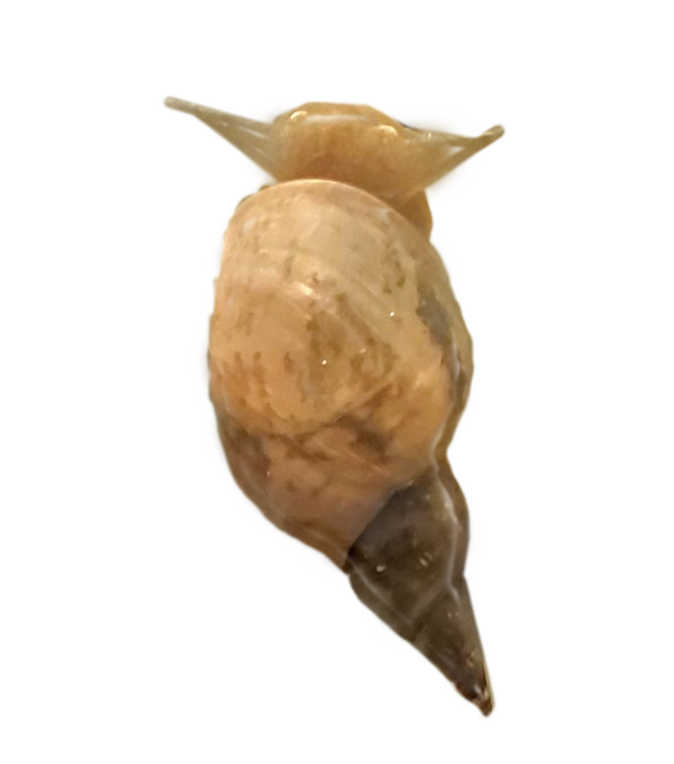
\includegraphics[width=\linewidth]{img/intro/lymnaea.png} 
	\caption{Imagen of \textit{Lymnaea Stagnalis}}
	\label{fig:snail}
	\end{minipage}
	\hfill
	\begin{minipage}{0.65\textwidth}
		\centering
		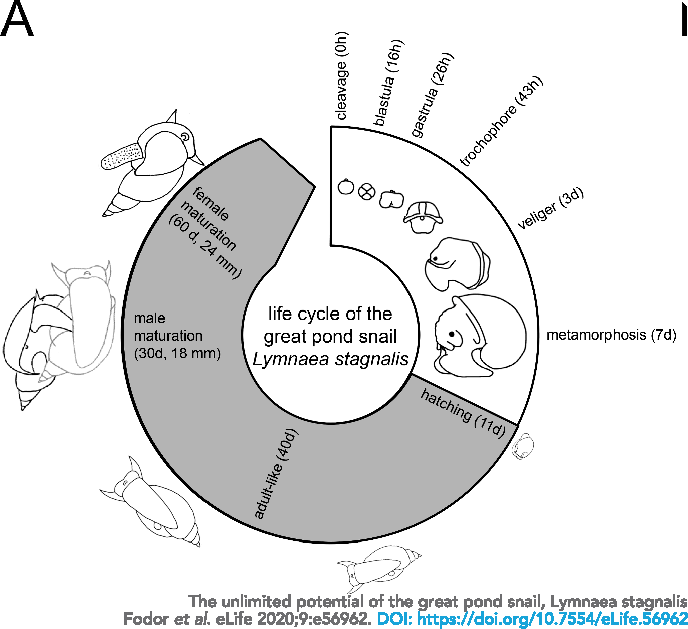
\includegraphics[width=\textwidth]{img/intro/lymnaea_life_cycle.pdf}
		\caption{Representation of \textit{L. stagnalis} life cycle. Figure 2A from \cite{fodor_unlimited_2020} (\href{http://creativecommons.org/licenses/by/4.0/}{Creative Commons license}).}
		\label{fig:lymnaea_life_cycle}
	\end{minipage}
\end{figure}

 From that point on, it has been key in other fields as host-parasite or genome editing. This last field is thanks to the short and well studied life-cycle in \textit{L. stagnalis} (see Fig. \ref{fig:lymnaea_life_cycle}), as well as the easiness to lab-bread them, without losing its main characteristics through generations \parencite{noland_observations_1946}. Recordings and analyses in this work are framed in the study of neural activity in it central nervous system (CNS). \textit{L. stagnalis} CNS is composed by 11 ganglia that conform the system: symmetrical pairs of buccal, pedal, cerebral, pleural and parietal, and a single visceral ganglia (see Sec. \ref{sec:lymnaea morphology}). We will focus specially in its feeding CPG, that by a distributed combination of motor- and inter-neurons allocated mainly in buccal and cerebral ganglia, produce a rhythmic pattern movement that allows feeding in three phases (protraction, rasp and swallow). Beyond this study of the CPG, we will work on the giant neurons located in the right parietal ganglia (RPG), enhancing the high-voltage (up to 80mV) and slow activity (30 to 100 ms per spike) to analyze in detail the action potential dynamics. 


\section{Neural stimulation}
\subsection{Stimulation techniques}

Neural stimulation have been an essential aspect in the study of neural dynamics, allowing the modulation of the neural system to explore, reproduce and alter its dynamics for their study. There are several techniques to produce the stimulation, we could classify them in chemical --using chemical components to block/enhance neural mechanisms--, electrical --injecting current in the cell membrane or nerves-- or optical --where neurons or circuits are stimulated though a illumination process. In this thesis,  we focus in the last two. In the electrical techniques, since the firsts applications of electrophysiology by \cite{neher_single-channel_1976} and the subsequent apparition of patch-clamp technique \cite{hamill_improved_1981}, many different techniques have been developed, for distinct systems. Voltage-clamp and patch clamping modified the paradigm in physiology and basic medicine in the study of the cell membrane dynamics with an exceptional detail that still today is heading ranges of precise recording and stimulation \parencite{hamill_improved_1981}. To Voltage-clamp followed variations such as dynamic-clamp, that enhances the electrophysiology possibilities by combining it with the possibilities of computing through a closed-loop protocol in real-time \parencite{nowotny_dynamic_2022}. This allows implementing specific algorithms to intervene the neural activity and test it to different approaches \parencite{chamorro_generalization_2012}. 
Regarding optical stimulation, a novel and widespread technique is opto-genetics, that by genetically modifying the animals, neurons are reactive to light and have had great achivements in the last decades using for both stimulation and exploration \parencite{chen_roles_2022}. Other example still understudy is near-infrared laser, a novel technique that will be explored in detail along this thesis. This technique have proven its potential for neuronal stimulation in different systems such as the hippocampus \parencite{liang_temperature-dependent_2009}, spinal ganglia in the cochlea \cite{goyal_acute_2012, barrett_pulsed_2018, brown_thermal_2020} and other systems \parencite{shapiro_infrared_2012, cayce_infrared_2014, begeng_activity_2022}.

%
%Apart from their possible subsequent aplication in clinical application, the use of these techniques for basis science is essential for a clear understanding of their implications, the biophysical mechanism they are able to alter and its safety range, and also for a wide understanding of the brain functioning.

\subsection{Neuromodulation and its need for clinical applications}


Beyond the necessity for neural stimulation in basic research to understand and explore the brain signaling and dynamics, there is a direct social impact for neural stimulation in clinical applications. In this context, Neuromodulation is an area of medicine involving many specialities that can be defined as "the science of how electrical, chemical and mechanical interventions can modulate distinct models of the nervous system function [and it is] inherently non-destructive, reversible, and adjustable" \parencite{krames_neuromodulation_2009}. This field is so important due to its possibilities in brain disorder treatments, for functional stimulation but also by the long-term modulation through neuronal plasticity. Neuromodulation can be classified, depending on the technology used for it, as invasive or non-invasive. Invasive technologies are those that require a direct interaction with the living system, which causes harm, e.g. including surgery. A well-known example of this type is deep-brain stimulation (DBS), this technique has been effectively used to treat movement disorders by electrically stimulating the brain at certain brain areas after implanting a device \parencite{limousin_long-term_2019, hariz_deep_2022}. In the case of non-invasive neuromodulation, we can find transcranial magnetic stimulation (TCM), that by electric fields stimulates certain areas of the brain, successful for example in the treatment of depression or obsessive compulsive disorder \parencite{valero-cabre_transcranial_2017, clarke_patients_2018}. Each type of technique has its own advantages, invasive techniques are usually more precise in space and time, whereas non-invasive techniques provide more flexibility and adaptability to different patients and the spreadness of the technique. In this context, the optical techniques discussed for stimulation in basic research have been rising in popularity also for clinical applications. 












	% \chapter{Motivation and Objectives}\label{c-review}
During this work, we will analyze and explore neuronal activity focusing on its dynamics and following a bottom-up approach. In the state of art we discussed the importance of sequential dynamics, and how we can describe this sequentiality at different scales, from milliseconds (ionic channels) up to hours or days in terms of behavior or cycles. It is important to study neuronal dynamics at different levels to understand the mechanisms behind the information processing and the subsequent outputs. To explore sequential activation at cell levels, we will use intracellular recordings of single neurons and cells from the feeding CPG circuit of \textit{Lymnaea stagnalis} combining an experimental study with conductance-based models. In the case of the CPG sequential activity, we will characterize and quantify cycle-by-cycle the variability of the sequence intervals. Although this approach has not always been typical in these kinds of studies \parencite{anwar_interanimal_2022}, the assessment of the variability of sequence time-intervals can unveil important characteristics and constraints for the motor coordination \parencite{elices_robust_2019}. Bursting activity is a good case study for this, since it is usually easier to define the phases associated to the context based on the burst events. In this work, we will discuss the generalization of the presence of sequential dynamical invariants, discovered in the pyloric CPG \parencite{elices_robust_2019}, exploring them in the feeding CPG of \textit{Lymnaea stagnalis}, both in a computational model and in experimental recordings. We will explore the restrictions underlying the CPG but also the possible functional role of these restrictions under different cases of activation of the CPG, e.g., feeding initiated by the presence of food or feeding activity initiated even in the absence of food. 

On the other hand, we also reviewed in the previous chapter the importance of stimulation techniques to explore the neural dynamics and behavior but also for possible clinical applications. In the second part of this work, we will explore Continuous-Wave Near-Infrared (CW-NIR) laser, a novel technique for neuronal dynamics modulation. This optical stimulation has potential for effective modulation of neuronal dynamics, but its exact mode of action is not known yet. There are different hypotheses, each one pointing to different candidates being affected during signal modulation in the process of the signal modulation, such as calcium channels, capacitance or long-term process as mitochondria modulation, as well as different sources for the effect, as photo-thermal or photo-chemical effect. During this work we will characterize its effect in single neurons combining experimental and theoretical approaches to narrow down the possible candidates and the source of the effect. We will also present a novel approach for closed-loop stimulation to predict spikes and stimulate at different stages of the action potential generation. 

In summary the objectives of this thesis are:
\begin{enumerate}
    \item To explore the sequential nature of neuronal dynamics. 
    \item To analyze the feeding CPG of \textit{Lymnaea stagnalis} to provide evidence of the universality of sequential dynamical invariants found in the pyloric CPG.
    \begin{enumerate}
        \item To characterize the sequential invariants cycle-by-cycle in the bursting model. 
        \item To analyze intracellular recordings with spontaneous activity and with different rhythm initiation stimulations. 
    \end{enumerate}
    \item To study the restrictions of variability in the reproduction of neural models and circuits.
    \item Discuss the possible functionality of sequential dynamical invariants in robotics. 
    \item Test the capability of CW-NIR laser stimulation to modify neural activity. 
    \begin{enumerate}
        \item Characterization of the effect in the spike waveform dynamics. 
        \item Analysis of the ability to change spiking activity and circuits dynamics. 
    \end{enumerate}
    \item Study the possible candidates underlying the effect in model simulation. 
    \item Design and implement a new technique for the stimulation in closed-loop. 
\end{enumerate}

Understanding the sequential patterns at the level of CPGs and single neurons allows us to identify universal principles that can be applied to broader neural circuits and behaviors. The sequential dynamics explored in the first part of this thesis provide foundational insights into the intrinsic timing mechanisms that govern neural processes. By exploring novel modulator techniques, as near-infrared laser stimulation, we bridge the gap between neural dynamics and the necessary modulation techniques. Also, will allow the precise dissection of sequential activation at ionic-channels by the activity-dependent laser illumination. 

	% \chapter{Materials and Methods}
This section covers the general information for the materials and methods covered in this thesis and that are common for chapters \ref{c-invariants} and \ref{c-laser}. The methods here presented are also extended in those chapters when necessary.


\section{The neural system of \textit{Lymnaea stagnalis}}
\label{sec:lymnaea morphology}
The neural system of \textit{Lymnaea Stangalis} (the great pond snail) is shown in figure \ref{fig:lymn neural sys diagram}. As in some other mollusks, e.g. {\sl Clione}, the neural system is conformed by several ganglia, each of them controlling (mainly, but not exclusively) some specific function of the snail. Figure \ref{fig:lymn neural sys diagram} shows a labeled image of the different ganglia in this system. All ganglia in the neural system are paired and distributed symmetrically, except from the visceral ganglion (unique) and the parietal, that although symmetrical, the right parietal is larger than left parietal ganglion (see \ref{fig:lymn neural sys diagram}). All ganglia are interconnected by nerves (grey stripes in the image). As mentioned before, each ganglion has an associated behavioral task in the snail. From top to bottom: we find the buccal ganglia (upper pair), which control the buccal muscle involved in the processes of open-rasp-swallow, known as the feeding cycle, initiated by a CPG circuit contained in these ganglia. The two cerebral ganglia (right bellow) are involved in the activation and modulation of many circuits and processes, including the modulation from specific neurons in all ganglia. Located on the sides of the diagram, the pedal ganglia control the snail pedal movements as crawling or swimming, and they are originally joined. The pleural ganglia, which contain sensory neurons, are connected to the mantle. And finally, at the bottom of the diagram, we find the parietal ganglion, involved in the control of the gill (respiratory organ) and the olfactory organ, and the visceral ganglion, connected to organs such as the intestine, the heart, and part of the genital system.


\begin{figure}[h!]
	\minipage{0.45\textwidth}
	\centering
	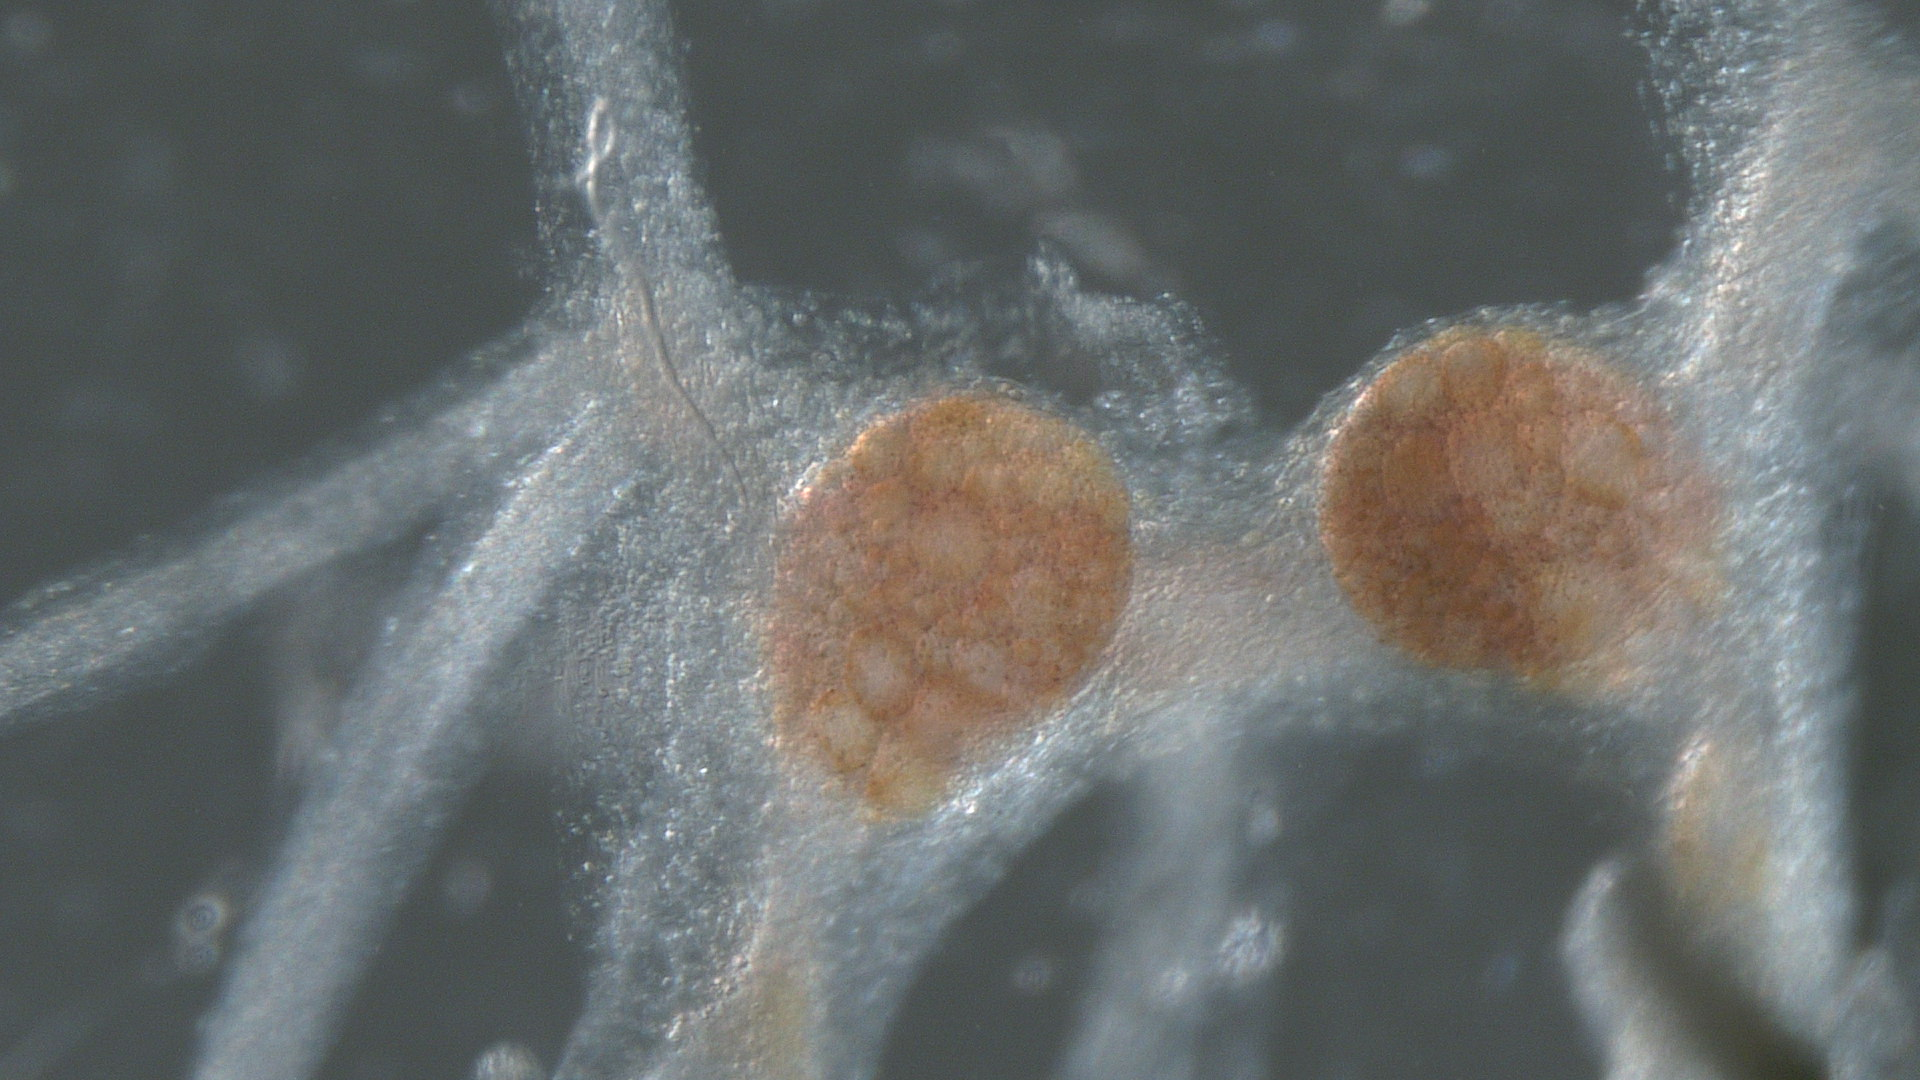
\includegraphics[angle=180,width=0.9\linewidth]{img/methods/preparation/buccal_ganglia.JPG}
	\caption{Lymnaea buccal ganglia.}
	\label{fig:buccal ganglia}
	\endminipage
	\minipage{0.45\textwidth}
	\centering
	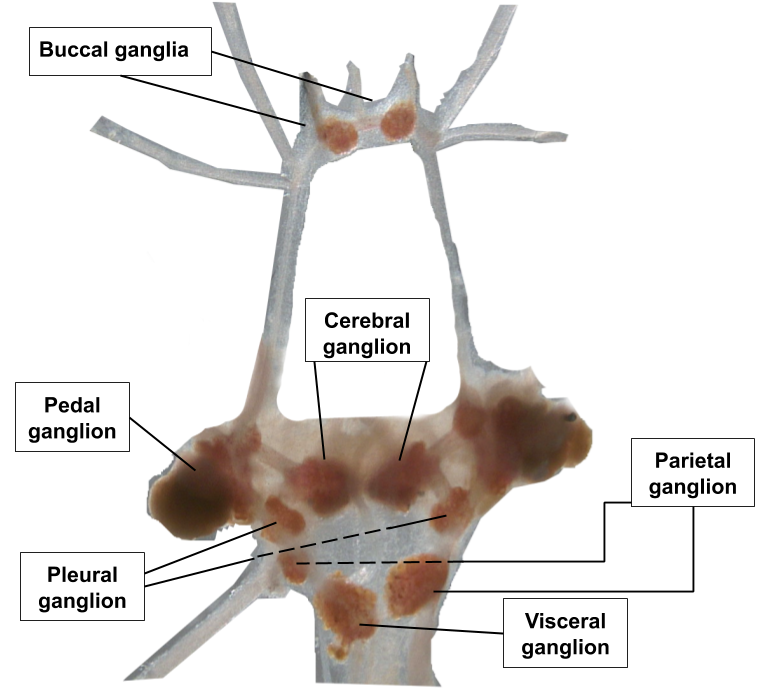
\includegraphics[width=\linewidth]{img/methods/CNS_diagram.png}
	\caption{Lymnaea nervous system diagram.}
	\label{fig:lymn neural sys diagram}
	\endminipage
\end{figure}

Neuronal recordings showed in this work are from the CPG in the buccal ganglia (see \ref{c-invariants}) and right parietal ganglia, containing large neurons with tonic firing (see \ref{c-laser}). Both ganglia are showed in detail in figures \ref{fig:buccal ganglia}.

%%%% In contrast to other systems functionality where motoneurons are CPGs neurons \cite{stomatogastric} ((page 5 review), in Lymnaea nervous system, CPGs and motoneurons are separated groups of neurons. 


\section{Feeding CPG in \textit{L. stagnalis}}
%
\subsection{Feeding CPG Model}
For our analysis of sequence interval variability we used the CPG model developed by Vavoulis et al. \cite{Vavoulis2007}. The model describes the activity of  three neurons conforming the CPG feeding system of the mollusk \textit{Lymnaea} (N1M, N2v and N3t cells) along with the modulator neuron SO, which has a key role in the CPG activity by regulating the feeding cycle duration. Each CPG neuron is associated to one specific movement in the feeding activity: protraction (N1M), rasp (N2v) and swallow (N3t) \cite{Benjamin2012}. During protraction, the buccal mass and radular move forwards on the food. During rasp, the radular begins to move back to get the food into the buccal cavity. During swallow, the mouth closes and the radular pushes the food into the esophagus.

The dynamics of the single neuron models are based on a Hodgkin-Huxley conductance-based formalism \cite{HODGKIN1952} describing active ionic channels with specific features to reproduce the observed waveform from experimental recordings in each cell.
The Vavoulis et al. description of the individual neurons considers a two-compartment model to represent the soma and the axon as  differentiated structures coupled by an axial resistance \cite{Vavoulis2007}. This separation of the soma and the axon is used to regulate the interaction between the fast and slow dynamics in the model. The slow dynamics are located the soma, whereas the fast dynamics are included in the axon compartment of the model. This distributed formalism is represented in Fig. \ref{fig:2 compartments}, where each circle represents either soma or axon, with a distinct ionic current distribution. The description of the compartment dynamics is provided by equations (\ref{eq:soma}) and (\ref{eq:axon}) for soma and axon, respectively: 
%Cambios
%being \(i_X\) a different channel for each neuron in the CPG (N1M,N2v,N3t).

% which is usually represented in models as \(i_{e1} = g * (V_1 - V_2)\), where $V_1$ and $V_2$ represent the voltage in each of the two compartments and $g$ is the coupling conductance, the inverse of the axial resistance and $i_{e1}$ is the current that flows into one compartment from the other.
\begin{equation}
    \tau_m\frac{dV_S}{dt} = i_{inj} - i_{L,S} - i_X - i_{ec,S} - i_{syn} \\,
    \quad with \quad i_X = [i_{ACh},i_{NaL},i_T]
    \label{eq:soma}
\end{equation}

\begin{equation}
    \tau_m\frac{dV_A}{dt} = -i_{L,A} - i_{NaT} - i_K - i_{ec,A}
    \label{eq:axon}
\end{equation}

\begin{figure}
\centering
\begin{subfigure}[t]{0.5\textwidth}
\includegraphics[width=\textwidth]{img/methods-paper-modelo/figure1a.eps} 

\caption{} \label{fig:2 compartments}
\end{subfigure}
\hfill
\begin{subfigure}[t]{0.49\textwidth}
\centering
\includegraphics[width=\textwidth]{img/methods-paper-modelo/figure1b.eps} 
%TODO FIX
\caption{} \label{fig:CPG diagram}
\end{subfigure}
 
 \caption{\textbf{Panel (a)}. Ionic channel distribution in the two-compartment description for the individual neurons in the Vavoulis et al. model \cite{Vavoulis2007} used in this study. At the soma: $I_{ACh}$, acetylcholine ionic channel; $I_{NaL}$, slowly inactivating sodium ionic channel;$I_T$, low-threshold calcium current; $I_{inj}$, injected current; $I_{L,S}$, leakage current in the soma; $I_{syn}$, synaptic current. At the axon: $I_{NaT}$, fast inactivating sodium current; $I_K$, delayed rectifier potassium current; $I_{L,A}$, leakage current in the axon. The electrical couplings are described as $I_{ec,S}=g_{ec}(V_S-V_A)$ and $I_{ec,A}=g_{ec}(V_A-V_S)$, respectively, being $g_{ec}$ the coupling conductance. The color for each $I_X$ current represents the CPG neuron that includes it at the soma,  N1M, N2v and N3t, respectively, as shown in panel (b). \textbf{Panel (b)}. Connection scheme for the {\sl Lymnaea} feeding CPG circuit model. For details on the ionic channel current descriptions and associated parameters, see \cite{Vavoulis2007}. The colors indicating each neuron in the circuit match those in the representation of their corresponding somatic membrane potential traces throughout the paper. 
}
    
    % \label{fig:2 compartments}
\end{figure}


\vspace{0.3in}

\noindent Here we follow the notation of~\cite{Vavoulis2007} where $\tau_m$ represents the time constant of the membrane (in ms) given by the ratio of the membrane capacitance (in nF) and the leakage conductance (in $\mu$S).  In equations (1) and (2), $i$ variables (given in mV) are the product of the corresponding currents (in nA) times the passive input resistance given in M$\Omega$.
%, $i=I*R$, where  $R$ is given in M$\Omega$.
% Añadir explicación de unidades********. 


The soma compartment contains a slow current $I_X$ whose ionic nature depends on the specific CPG neuron described (see Fig.~\ref{fig:2 compartments}). Thus, $I_X$  represents one channel, either $I_{ACh}$, $I_{NaL}$ or $I_{T}$, responsible of the specific slow dynamics associated with neurons N1M, N2v and N3t, respectively.  Along with the slow ionic channel and the leakage channel  $I_{L,S}$, the soma compartment also receives the synaptic current $I_{syn}$ and the injection current $I_{inj}$. All currents are explained in detail below.
%TODO al final Leakage no se pone aqui?

%A more extended explanation of these channels and the property they produce is . Along with this slow activation channels, there are also found in the soma $i_{inj}$, an injected current, and $i_{syn}$ a synaptic input that is widely explained below. These are also represented in figure \ref{fig:2 compartments}

On the other hand, fast channels are part of the axon compartment: a fast inactivating sodium current $I_{NaT}$ and a delayed rectifier potassium current $I_{K}$. These channels, along with the axon leakage channel  $I_{L,A}$ are also represented in Fig.~\ref{fig:2 compartments}, for their detailed description see~\cite{Vavoulis2007}. 


% ***Descripción breves de corrientes en terminos de cuales son lentas y rápidas con referencia a la Fig.1
% y la i_x

The model cells as described above are not endogenously bursters. To achieve a realistic bursting activity in each neuron, a distinct constant value of  \(i_{inj}\) is applied to the cells. %  Values of \(i_{inj}\) used in this study to obtain realistic bursting activity. 
%TODO añadir " in the circuit".

 The CPG topology scheme is shown in Fig. \ref{fig:CPG diagram}, where the connections between neurons are represented by dashed or solid lines, depending on whether the connection is slow or fast, respectively, and filled or empty circles at their end denoting the direction and the effect on the postsynaptic neuron: excitation (empty circles) or inhibition (filled circles).
Individual neurons following the previous description are connected by graded synapses, defined by equations (\ref{eq:syn1}-\ref{eq:syn2}) \cite{Vavoulis2007}:

% \begin{equation}
%     i_{syn} = \sum_j \gamma_{syn,j} s_j (V_S - E_{syn,j})
%   \label{eq:syn1}
% \end{equation}
% % TODO FIX
% \begin{equation}
%     \frac{ds_j}{dt} = \frac{r_{j}-s_j}{\tau_{syn,j}}
% \end{equation}

% \begin{equation}
%   \frac{dr_j}{dt} = \frac{r_{\infty,j}-r_j}{\tau_{syn,j}}
% \end{equation}

% \begin{equation}
%     r_{\infty,j}=\frac{1}{1+e^{(-40-V_{pre_{V_S}})/2.5}}
%      \label{eq:syn2}
% \end{equation}


\noindent where index $j$ runs over all presynaptic neurons and \(\gamma_{syn,j}, E_{syn,j},\tau_{syn},V_{pre_{V_S}}\) are the product of input resistance and maximal synaptic conductance, the synaptic reversal potential, the synaptic time constant and the presynaptic potential, respectively.
%cambio

Together with the effect of the distinct connections conforming the circuit, the neuron dynamics in this model is shaped by the ionic channels at each cell and their associated parameters. The resulting triphasic CPG rhythm with distinct voltage waveforms of spiking-bursting activity is displayed in Fig. \ref{fig:model simulation}, where the effect of the connections in building the phase between neurons can also be observed. The traces correspond to a simulation of the complete circuit model, i.e., all connections shown in Fig. \ref{fig:CPG diagram} are active. 


\begin{figure}[h!]
    \centering
    \includegraphics[width=\linewidth]{img/methods-paper-modelo/figure2.eps}
    \caption{Triphasic feeding rhythm as produced by the circuit CPG model described in Fig. \ref{fig:CPG diagram}. In this simulation, $i_{inj}$ values applied to each neuron are 8.5, 6, 2 and 0 mV, respectively.}
    \label{fig:model simulation}
\end{figure}

The distinct waveforms for each neuron are mainly due to their specific ionic channel dynamics. On the one hand, N1M voltage characteristics are provided by an acetylcholine sensitive channel (\(i_{ACh} = 200 * p^3 * (V_S + 30)\)), which causes the gradual spiking frequency increase as well as the visible plateau, i.e., the slow wave is sustained before hyperpolarization. On the other hand, N2v has a slowly inactivating sodium channel (\(i_{NaL} = 2 * p^3 * q^3 * (V_S-55)\)), which causes the slow depolarization in this neuron. N2v neuron has a lower spiking frequency caused by the conductance value given for the axial $g_{ec}$ linking the two compartments, which is much lower in this cell. Finally, the N3t neuron has the particularity of a post inhibitory rebound, which generates an initial fast spiking followed by a decrease in the firing rate as the burst evolves. This latter property is caused by a low-threshold calcium channel (\( i_T = 3.27 * p^3 * q *(V_S-80)\)).

%cambios
In contrast to the N1M, N2v and N3t neurons of the CPG, the model of the SO neuron has no \(I_X\) channel, so its activity is the result of the combination of the common ionic channels in the axon and the soma.
% ****no se dice nada de la SO ****

\subsection{Inducing variability by current injection}
\label{subsec:inj protocol}
The spiking-bursting activity of the model CPG neurons can be modulated by using an additional current injection on each cell, implemented in the \(i_{inj}\) term of equation (\ref{eq:soma}), as performed in many experimental protocols. Depending on the value % of the current 
applied,%TODO current o value applied?
% the corresponding neuron dynamics changes. While for N2v a change in this current injection corresponds to a change in burst frequency (i.e. the number of bursts increases/decreases), for the rest of the neurons in the model (N1M, N3t and SO) a change in \(i_{inj}\) affects their burst duration. %%TODO ????
the corresponding neuron dynamics changes. While for N2v a change in this injection corresponds to a change in burst frequency (i.e. the number of bursts increases/decreases),
for the rest of the neurons in the model a change in \(i_{inj}\) affects burst duration for N3t and SO,  and the length of the depolarization phase in N1M.


Whilst the single neuron model descriptions have no intrinsic variability, the effect produced by the modulation of the injected current in each neuron induces variability into the circuit, which allows characterizing the sequence intervals and the period, the associated robustness of the rhythm and the presence of dynamical invariants. Such stimulation has been used previously in the living circuit, as reported by Elliot et al. \cite{Elliott1991}. The authors of this work showed that it is possible to activate the feeding CPG with variability caused by current injection into individual cells in the circuit. CPG rhythms obtained under this type of stimulation differ depending on which neuron is being stimulated. 

% Even though this CPG model do not present intrinsic variability, thanks to the current \(i_{inj}\), variability is induced into the model, effectively changing burst duration. This current injection has also been used in Lymnaea preparation in living elements, stimulating N1M and SO, obtaining rhythm. Neural sequences obtained after the stimulation differ one another depending on which neuron is being stimulated. 

By varying the current injected into N1M, its burst duration is kept nearly constant, but its depolarization phase before the spiking activity begins becomes longer. Since N3t is the neuron fitting in the sequence in that phase (see Fig. \ref{fig:model simulation}), it also increases its burst duration, being the most variable one in the CPG rhythm. 

When %current 
value \(i_{inj}\) is increased on neuron SO, its burst duration becomes longer. Since SO has a modulator effect over N3t and N1M, it also alters the burst duration of these two neurons.

Neuron N3t also shows variable burst duration when an evolving current is injected. When \(i_{inj}\) increases on N3t, its burst duration increases, elongating the N1M depolarization phase.  

Finally, when current is applied to N2v the effect on its burst duration or the burst duration of the rest of the neurons is rather small. However, \(i_{inj}\) % current 
modulates N2v burst frequency through the hyperpolarization phase. 

%cambios
Therefore, we used a current ramp protocol to induce variability in the CPG model defined as follows: a ramp variable $c$, which controlled the current injection value ($i_{inj}=c$) %TODO
on the neuron being stimulated, was increased from a minimum to a maximum value, and then decreased back to the initial value. This was repeated twice in each simulation. The ramp variable was modified with a fixed step value every 4.6 seconds (the approximate duration of two N3t bursts).
% occurrence of each two bursts in N3t neuron (every 5 seconds). ***discutimos esto, es cada burst o cada dos como dice abajo, quizás convendría decir que corresponde a ese tiempo en el modelo sin estímulo. Por otro lado el lector se podría preguntar por qué no es una rampa de subida y bajada prestablecida en el tiempo***
The minimum and maximum $c$ values were different in each cell and were %chosen experimentally using model simulations 
tuned to generate realistic spiking-bursting behavior. %cambios : añadir por si experimentally no se entiende bien? depending on the effect of the injected current on the neuron to ensure robust burst generation in all neurons 
%Note that this variable $c$ value which goes through the different values in the ramp is $i_{inj}$ value, replacing the constant value of this current.
All parameters used for the simulation analyses reported in this paper are summarized in Table \ref{table:inj values}. An example of how this ramp current injection affects the rhythm is shown in Fig. \ref{fig:complete ramp example}. 
%cambios : quitar esta frase e indicarlo en seccion 2.3
% The rest of model and synapse parameters used to simulate the model are the same ones specified in the paper that describes the Vavoulis et al. model \cite{Vavoulis2007}.


\begin{table}[h!]
\centering
\begin{tabular}{c|cccc|c|ccc|}
\multirow{2}{*}{\textbf{\begin{tabular}[c]{@{}c@{}}Neuron\\ stimulated\end{tabular}}} & \multicolumn{4}{c|}{\textbf{\(i_{inj}\) value}}                 & \multirow{6}{*}{} & \multicolumn{3}{c|}{\textbf{Ramp values ($c$)}}   \\ \cline{2-5} \cline{7-9} 
                                                                                      & \textbf{SO} & \textbf{N1M} & \textbf{N2v} & \textbf{N3t} &                   & \textbf{Min} & \textbf{Max} & \textbf{Step} \\ \cline{1-5} \cline{7-9} 
\textbf{N1M}                                                                          & 8.5         & $c$            & 2            & 0            &                   & 0            & 10.5         & 0.5           \\ \cline{1-5} \cline{7-9} 
\textbf{N3t}                                                                          & 9           & 10           & 1            & $c$            &                   & 0            & 5            & 0.25          \\ \cline{1-5} \cline{7-9} 
\textbf{SO}                                                                           & $c$           & 10           & 1            & 4            &                   & 8.2          & 13           & 0.25          \\ \cline{1-5} \cline{7-9} 
\end{tabular}
\caption{List of \(i_{inj}\) values that yield realistic bursting rhythms for each neuron in the model CPG used in the stimulation protocols reported in this paper. The left section of the table displays the \(i_{inj}\) values applied to each neuron (columns) during each simulation condition (rows). Ramp values on the right section refer to the minimum and maximum values of the ramp variable $c$ in each simulation, increasing \(i_{inj}\) in the specified step every 4.6 seconds (the approximate duration of two N3t burst) to induce variability.} \label{table:inj values}
\end{table}


\begin{figure}[h!]
    \centering
    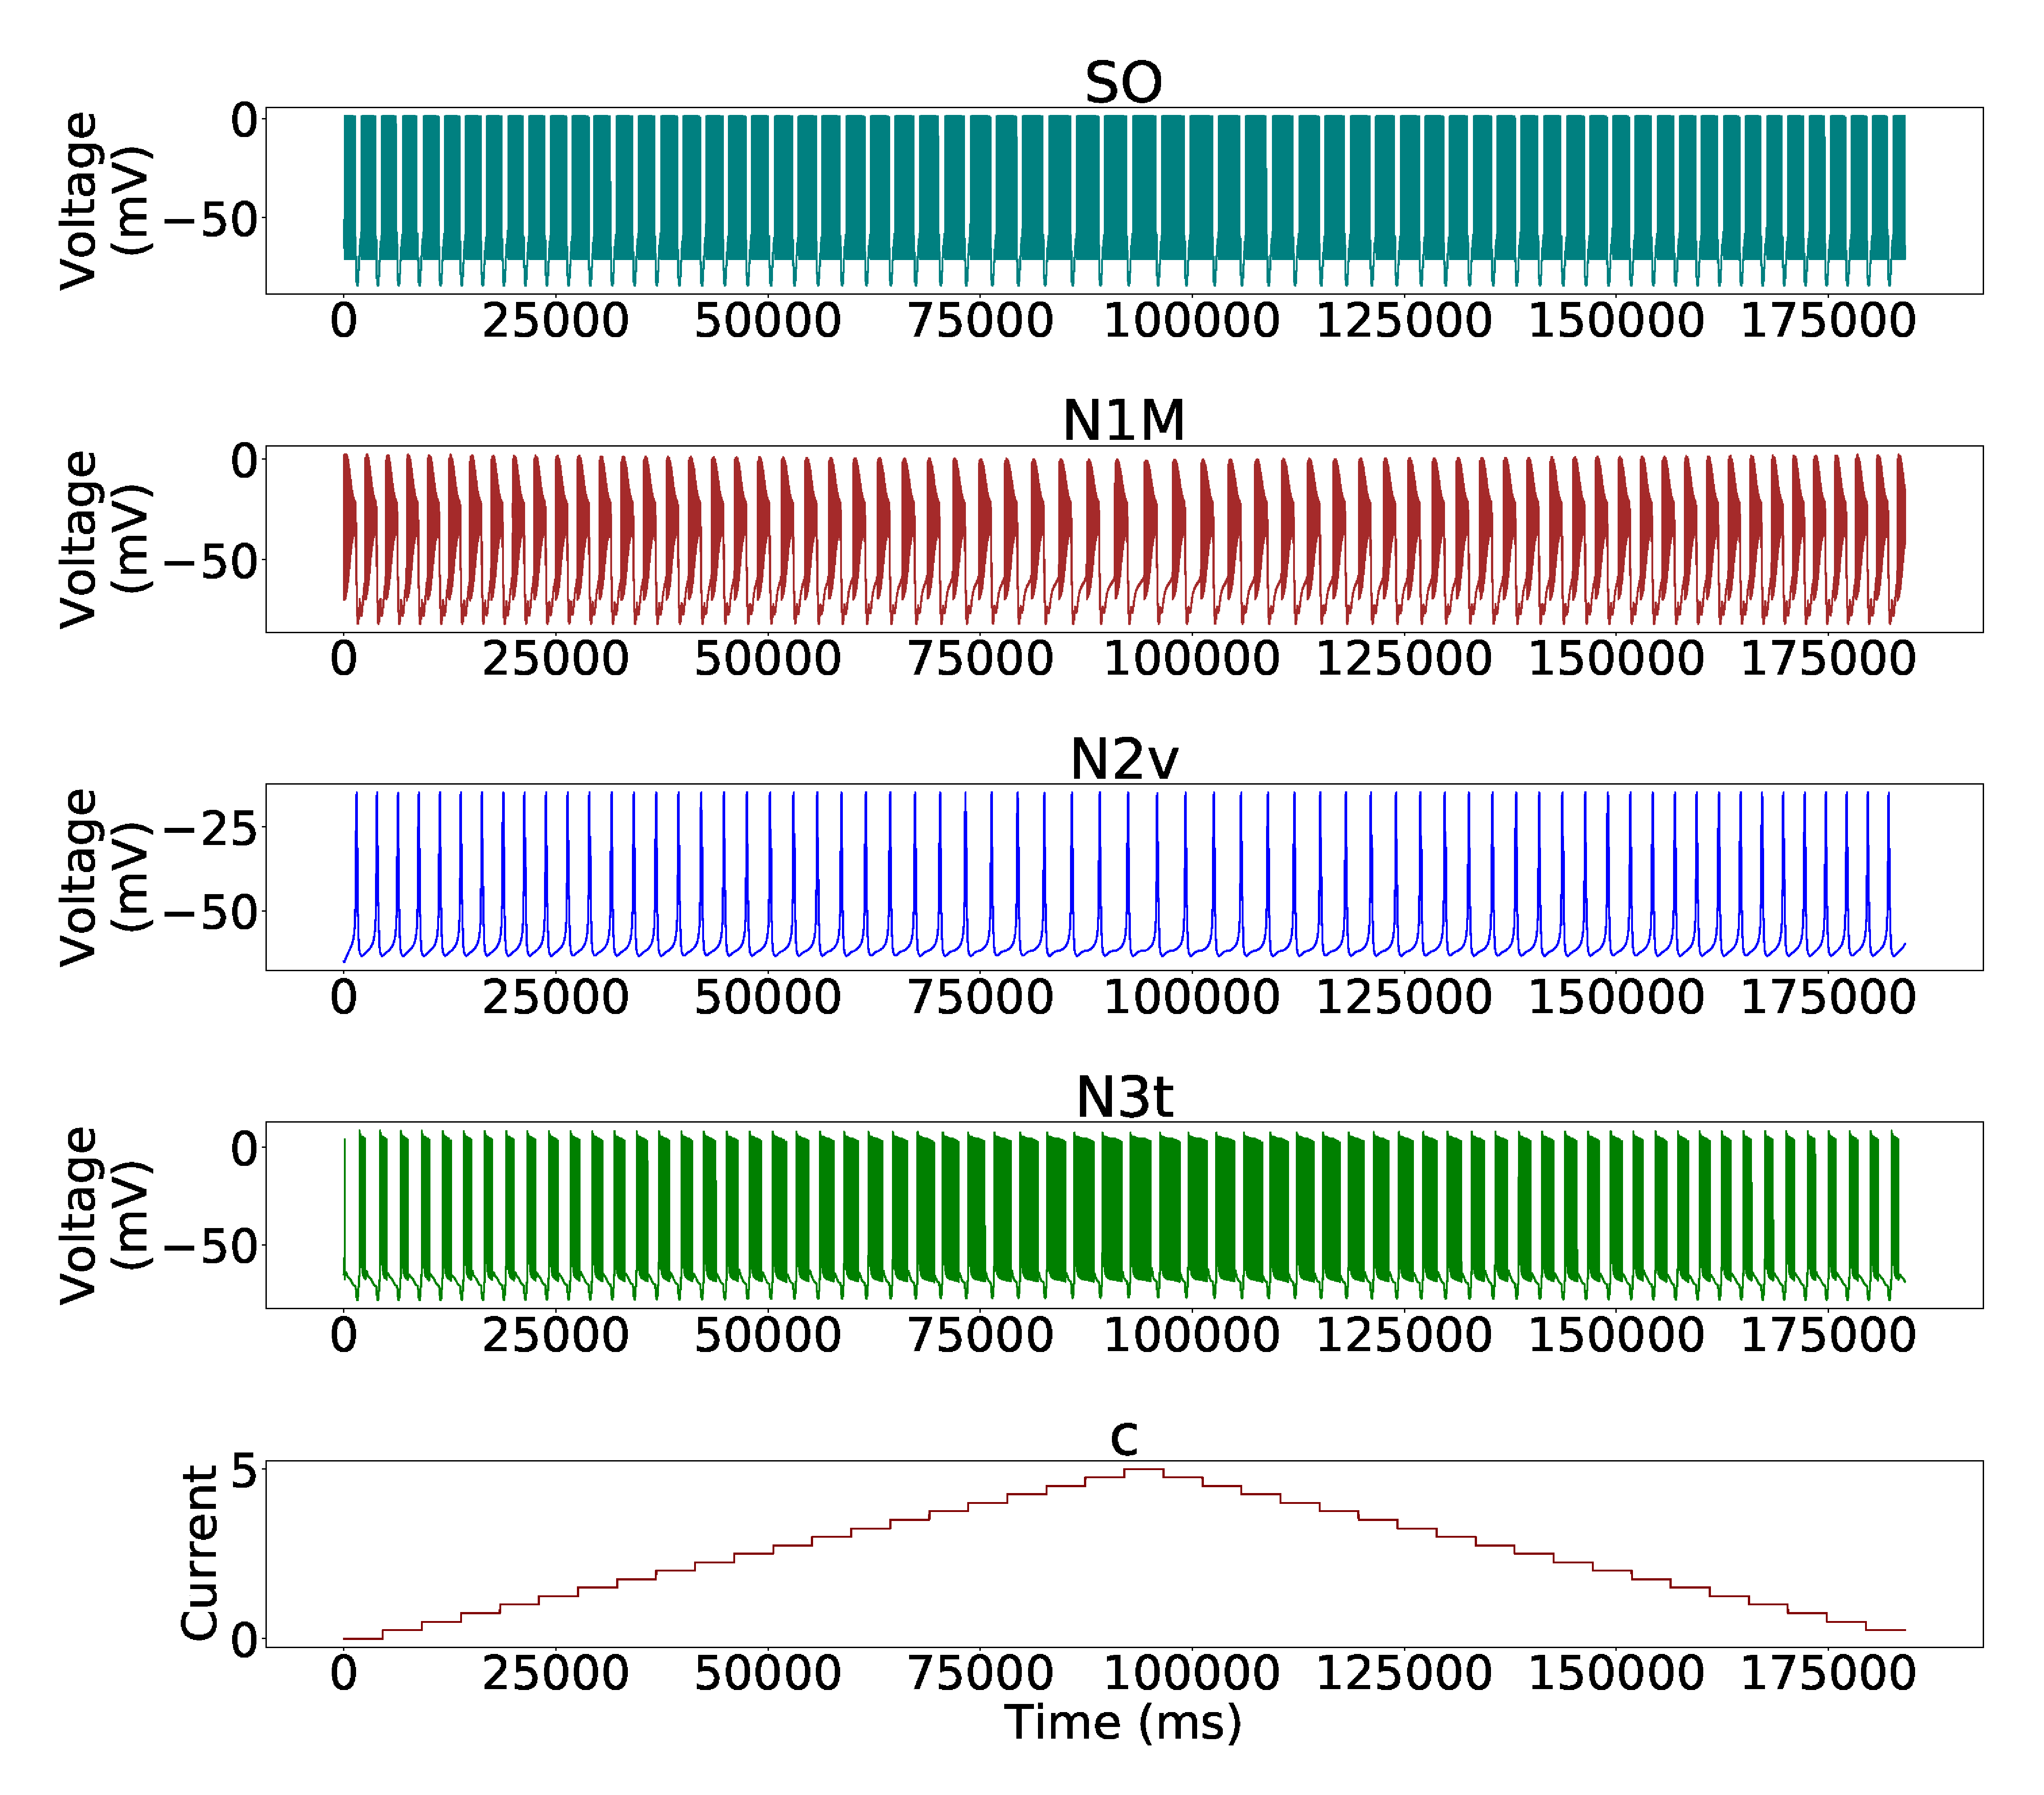
\includegraphics[width=\textwidth]{img/methods-paper-modelo/figure3.eps}
    \caption{Illustration of the CPG activity when a current ramp \(i_{inj}\) is applied to N3t. Variability in the sequence intervals was induced by applying two consecutive ramps as the one shown in this figure into different cells.  }
    \label{fig:complete ramp example}
\end{figure}


\subsection{Model simulation specifications and statistical analysis}
Simulations of the Vavoulis et al. model \cite{Vavoulis2007} were implemented in C++. The code of the feeding CPG model implementation is available at \url{https://github.com/GNB-UAM/CPG-feeding-Lymnaea}. Each simulation had the duration of two consecutive cycles of up and down ramps as the one shown in Fig. \ref{fig:complete ramp example} using the parameters described in Table \ref{table:inj values}. The number of bursts in each simulation was approximately 140 (this number slightly depends on the neuron stimulated). Parameter values such as reversal potentials and synaptic conductances were the same ones specified in \cite{Vavoulis2007}.
The statistical analysis was done in Python 3.6. For the temporal variability study, first the spikes were detected %\sout{using a threshold protocol. Due to the drift in the spike amplitude during the bursting of some of the neurons (as N2v), the spike detection was performed over the $1^{st}$ derivative of the signal}
using the change in the derivative during the computation of the model along with a threshold condition. Then, bursts were identified from the temporal structure of the spikes, and intervals were characterized by the timing of the first and last spike in each burst. 

Thus, all intervals defined below in section \ref{subsec:intervals} were measured and their variability was characterized by statistical analysis tools, i.e,  boxplots and linear correlations. For the boxplots, the Python library matplotlib.pyplot used each cycle-by-cycle interval duration. Linear regression from sklearn Python library was used to quantify the relation of the sequence intervals to the instantaneous period of each cycle. 

\subsection{Time references, intervals and CPG sequence}
\label{subsec:intervals}
The variability study addressed here is based on the characterization of  cycle-by-cycle intervals in the rhythm produced by the model CPG. % In order to explore possible dynamical invariants on this \textit{Lymnaea} feeding CPG, the intervals here analyzed follow the ones defined for the stomatogastric CPG dynamical invariants \cite{Elices2019}. Hence, based on the burst duration we will have in each cycle all corresponding burst duration intervals and some derived intervals obtained by the combination of pair of neurons, as well as the period. The resulting intervals here analyzed are shown in figure \ref{fig:intervals}. 
In our analysis of variability, we assess the presence of linear relationships between the intervals that build the sequence and the cycle-by-cycle period to characterize and unveil similar dynamical invariants as those found in the stomatogastric CPG \cite{Elices2019}. 
%Hence, we characterize the intervals building the CPG sequence, including its period. 
%on the burst duration we will have in each cycle all corresponding burst duration intervals and some derived intervals obtained by their combination of pair of neurons, including the period.
% Hence, the burst events detected are going to be used to define three intervals in the trace of each individual neuron, and two additional intervals defined from the relation between two neurons. 
This is illustrated in Fig. \ref{fig:intervals}, where single neuron intervals and intervals defined between neurons are depicted. 
%cambios
The intervals here analyzed can be measured for any three neurons following a robust triphasic rhythm. In this paper N1, N2 and N3 represent the feeding CPG neurons simulated in the model: N1M, N2v and N3t, respectively.

% Here is the definition of each interval:
% \begin{enumerate}
%     \item \textbf{Burst Duration (BD)}, measured as the time interval between the first and the last spike of the burst (start to end in the trace of a given neuron).
%     \item \textbf{Inter burst interval (IBI)}, characterised as the difference between the last spike of a burst and the first one of the next one (end to start in the trace of a given neuron).
%     \item \textbf{Period}, which envelops the bursts from the three neurons, measured as the distance between the first spike of one burst in a neuron and the first spike of the next one on that neuron (start to start).
%     \item \textbf{NeuronX-NeuronY interval}, this interval is measured from the burst beginning of neuron X to the burst beginning of neuron Y (start X to start Y).
%     \item \textbf{NeuronX-NeuronY delay}, being the time lapse between the burst end of a neuron X and the burst beginning of neuron Y. (end X to start Y).
% \end{enumerate}

\begin{figure}
\centering
\begin{subfigure}[t]{\textwidth}
\centering
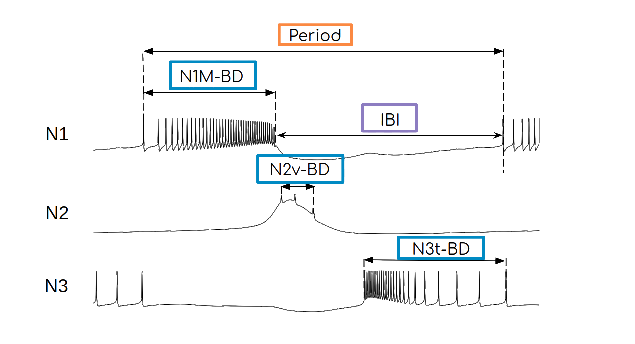
\includegraphics[scale=0.8]{img/methods-paper-modelo/figure4a.eps} 
\caption{} \label{fig:intervals_bd}
\end{subfigure}
% \hfill

    \vspace{1cm}
\begin{subfigure}[t]{\textwidth}
\centering
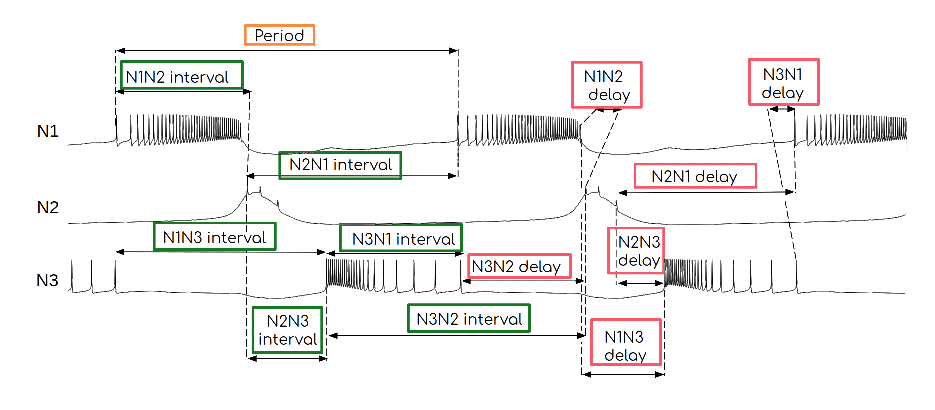
\includegraphics[scale=0.8]{img/methods-paper-modelo/figure4b.eps} 
\caption{} \label{fig:intervals_der}
\end{subfigure}
 
 \caption{\textbf{Panel A}. Individual neuron sequence interval definitions. Each BD label represents the burst duration, defined as the time interval from the first spike to the last spike in the neuron's burst. Period was measured as the interval from the first spike of N1 burst to the first spike of the next N1 burst, covering three phases %(N1M,N2v, N3t) 
 in relation to the activity of the other neurons. IBI represents the interburst interval, defined as the time from the last spike of a neuron's burst to the first one of the next burst in the same neuron.
    \textbf{Panel B}. Definition of intervals involving pairs of neurons. NXNY interval represents interval from NX start to NY start. NXNY delay represents interval from NX end to NY start. Period was measured from N1 start to N1 start, covering the three phases of the CPG rhythm.
    }
    
    \label{fig:intervals}
\end{figure}

\clearpage
\newpage



% ***quizás convendría añadir una subsección en los métodos diciendo cuál es la duración de las series temporales, las ráfagas que contienen y que se detectan los spikes para caracterizar los intervalos ciclo a ciclo. También que la variabilidad se caracerizó con boxplots del coeficiente de variación de todos los intervalos. Las figuras de los boxplots no parecen en porcentajes, los valores negativos habría que explicarlos en términos de que la fase de algunas neuroans se adelanta con respecto a lo definido en la figura 4 ***


%For the purpose of this study, the nerves employed for the extracellular recordings are the symmetrical pair of nerves coming out from the buccal ganglia, which were originally connected to the buccal mass. Since these nerves send out the impulses to move the muscles, the neurons whose activity is recorded in the extracellular signals are mostly motoneurons \cite{Benjamin1979a}, not the ones initiating the rhythm but the ones following the CPG neurons. It is important to localize these neurons in the extracellular recording for detecting the rhythm and the patterns. 
% On the one hand, the feeding rhythm in \textit{Lymnaea} is pretty slow and it is not always active. 

\subsubsection{Lymnaea feeding rhythm}

The feeding activity of the \textit{Lymnaea}, concerning the buccal mass, is classified in three main steps: Rest, protraction, rasp and swallow. This sequence of buccal movements in the snail is generated by the motor neurons distributed in the ganglia. Each of these phases is leaded by one interneuron from the CPG: N1M, N2v, N3t, and followed by the motoneurons associated to them. This is a complex distributed system where motoneurons do not exclusively follow the interneurons but are also implied in the feeding cycle activation \cite{staras_pattern-generating_1998}. In this circuit there are also some modulatory neurons implied such as SO neuron (in the same buccal ganglia) or CGC (in the cerebral ganglia). 

Hence, an initial resting state, where the CPG as well as the moto-neurons have no activity, may change due to a sensory input. This input, received in the presence of food or during hunger, is handled in the cerebral ganglia generating activity and changing the SO tonic spiking during resting (which was inhibiting the CPG) to a bursting mode, meaning the start of the feeding cycle.


This CPG circuit can be studied in a disected preparation, since snail's neurons are active after the isolation of the system. Specially, the CPG rhythm is maintained after its activation and it is generated in an autonomous way by the neurons in the circuit. However, due to the slow dynamics of the system and the nature of the experimental setting there are different ways to initiate the rhythm. In \textit{Lymnaea} literature, several options are proposed to solve this issue. The first solution is stimulating the neurons responsible for the initiation of the feeding rhythm, such as the SO modulator neuron on the buccal ganglia or also the CBC, CVs neurons, located on brain ganglia. Stimulating these cells usually activates the target circuits \cite{benjamin_distributed_2012}. However, the access to these neurons is not always easy and it might be necessary to keep them in constant stimulation. Another option for activation discussed in the literature is appliying octopamine. Some neurons in the buccal ganglia are sensitive to octopamine and, as a result, this procedure activates the rhythm \cite{vehovszky_octopamine-containing_2004}. Alternatively, in a semi-intact preparation, it can be applied sucrose to activate the rhythm \cite{vavoulis_computational_2007,vehovszky_octopamine-containing_2004,straub_endogenous_2002}. As a foresighted option, controlling the snails' feeding and selecting the first animal approaching the food seems to be effective for obtaining the feeding rhythm, with up to 80\% of success \cite{Elliott1991}.\todo{del tfm, quitar?}




\section{Electrophysiology in \textit{Lymnaea Stagnalis}}

\label{subsec:preparation}
In this thesis, intraceullular neuronal recordings have been carried out in the mollusk \textit{Lymnaea Stagnalis}. Beyond the advantages of invertebrates discussed in section \ref{c-intro-invertebrates} -- its easy accessible neural system, the size and resistance of its neurons to electrode impaling, the great pond snail's neural system is detailed described and so it is the feeding CPG which has been the model of study for chapter \ref{c-invariants} in this work. Also its slow dynamics, are convenient when studying the sequential evolution of the modulation, as in the case of the laser stimulation described along chapter \ref{c-laser}. 

The technique followed for the neural activity acquisition was intracellular recordings with filled with 3 M $KCl$ sharp electrodes, % in Figure \ref{fig:membranepotential recording} there is a scheme of the potential measurement. Está en la intro.
 In this technique, a glass micropippete penetrates the cell to record its activity, with a minimal damage on the cell, and the membrane potential is then recorded using a DC amplifier (ELC-03M, NPI Electronic, Hauptstrasse, Tamm, Germany). Micropippetes were pulled using a Sutter Instruments puller (Model P-97) (see Figure \ref{fig:electrode}). Membrane potential was recorded and recordings were acquired at 10 KHz using an A/D board (PCI-625 with a BNC-2090A DAQ device, National Instruments).

To facilitate the access to the cell, the sheath above it was reduced using protease (Sigma XVII) over the ganglion for $\sim$1 min and then washed with fresh saline. In order to record cell signals extra- and intracellularly, it is necessary to have full access to the neural system. Although there is an option to keep the buccal mass and do a semi-intact preparation \parencite{staras_cellular_1999} in this work the neural system (ganglia and nerves) was fully isolated (see \cite{garrido-pena_tfm_2022} for more details). The preparation was immersed in a saline solution (in mM: 51.3 $NaCl$, 1.7 $KCl$, 1.5 $MgCl_2\cdot6H_2O$, 4.1 $CaCl_2\cdot2H_2O$, 5 $HEPES$, corrected to pH 7.8 with 4 $M$ $NaOH$). All procedures followed the European Commission and Universidad Autónoma de Madrid animal treatment guidelines.

\begin{figure}[hbt!]
	\centering
	\begin{minipage}{0.4\textwidth}
		\centering
		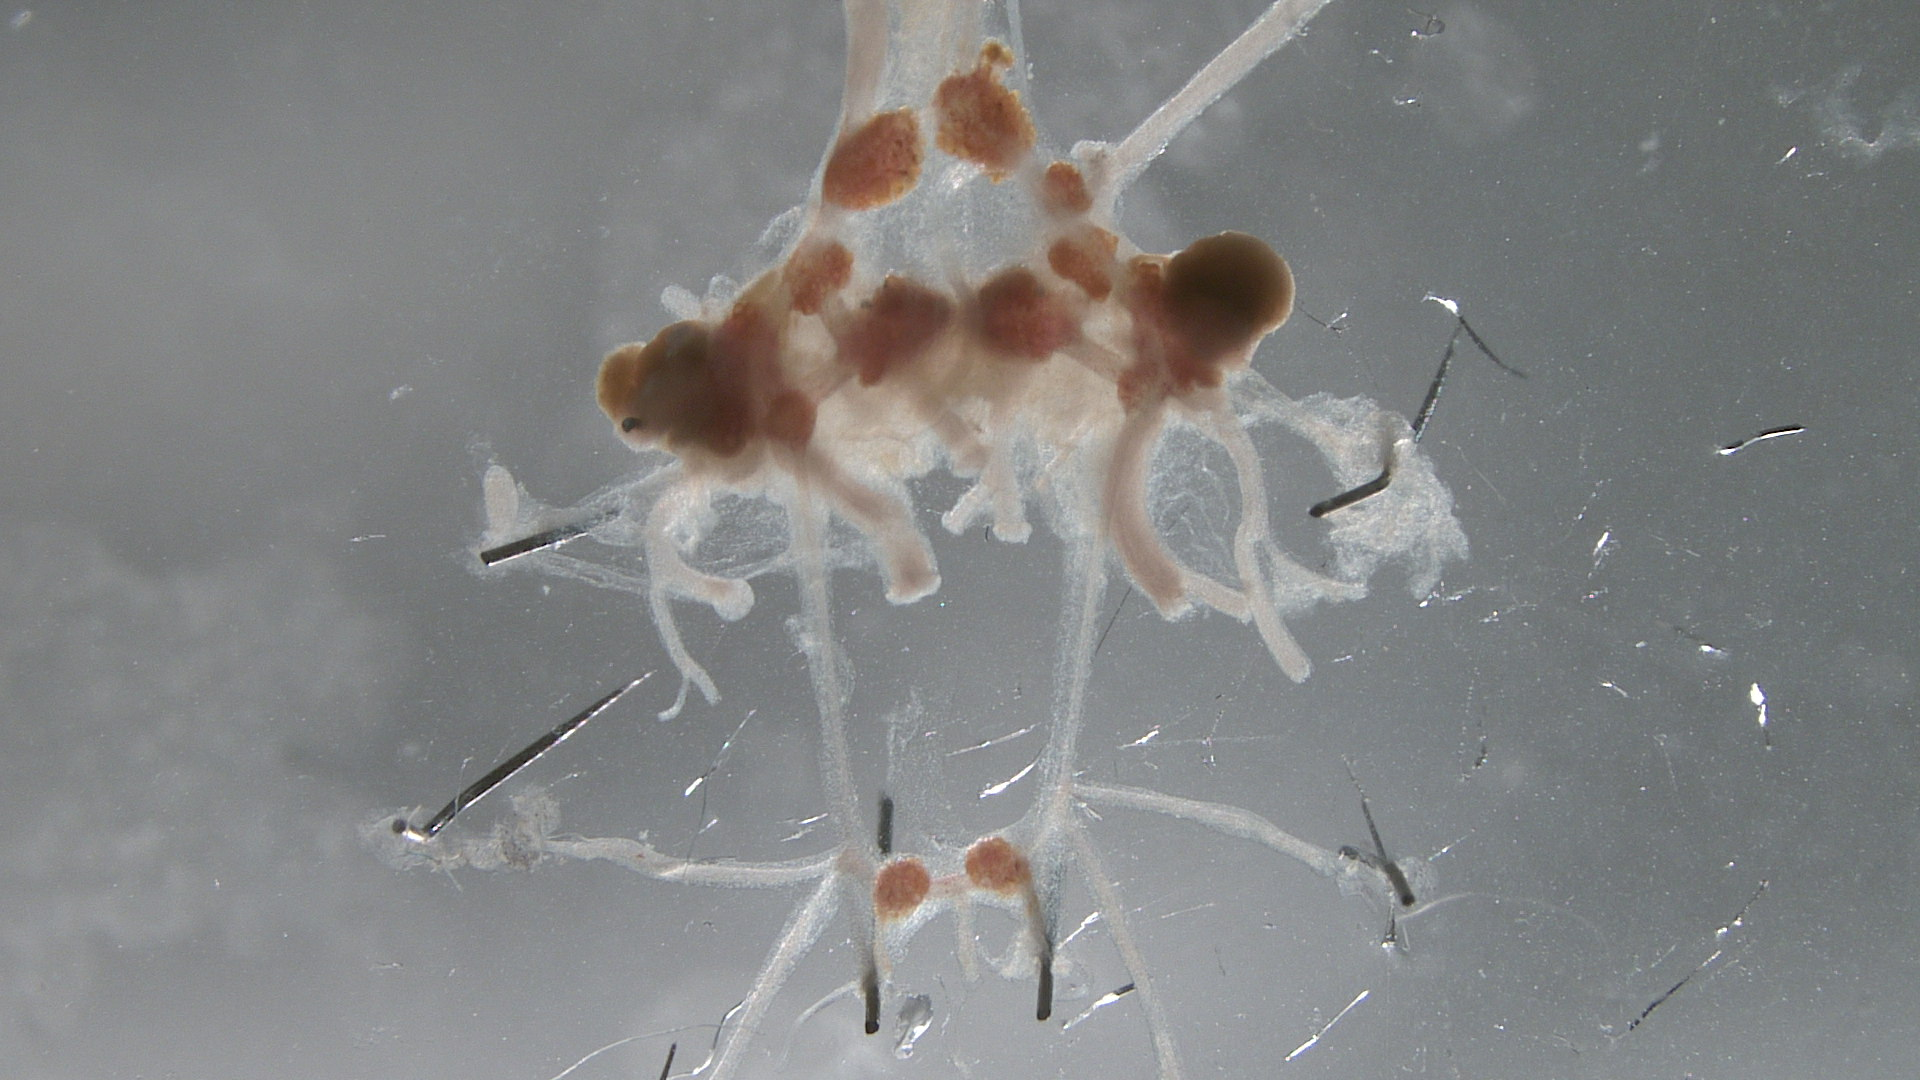
\includegraphics[angle=180,width=0.99\linewidth]{img/methods/IMG00027.jpg}
		\caption{\textit{Lymnaea stagnalis} neural system isolated.}
		\label{fig:preparation}
	\end{minipage}
	\hfill
	\centering
	\begin{minipage}{0.4\textwidth}
		\centering
		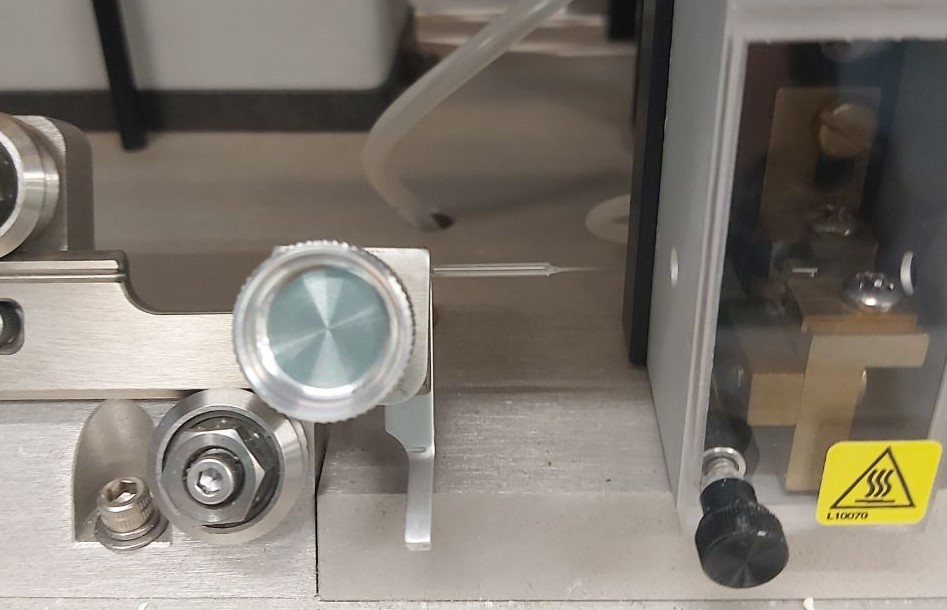
\includegraphics[width=0.99\linewidth]{img/methods/preparation/electrode4_zoom.jpg}
		\caption{Example of a sharp micro-electrode glass}
		\label{fig:electrode}
	\end{minipage}
\end{figure}


\section{Conductance based models}
For the theoretical analyses in this work, there have been used simulations of conductance-based models. As discussed in section \ref{computational neuroscience}, these models are based on a specific combination of ionic channels with a dynamic dependent on time that reproduces the Voltage value in the membrane at each time instant. There are many types of models and descriptions, depending on the specific combination of channels. Models used in this work, for both chapters \ref{c-invariants} and \ref{c-laser}, are description of neurons in \textit{Lymnaea stagnalis} for a neuron in cerebral ganglia, CGC \parencite{vavoulis_balanced_2010} and neurons in the feeding CPG in the buccal ganglia --SO, N1M, N2v, N3t, \parencite{vavoulis_computational_2007}. The first one, simulates a tonic firing and shoulder shape spike waveform, similar to the activity in some neurons in the right parietal ganglion. The second model is a detailed description of the CPG circuit with a combination of two-compartments neurons and a gradual synapse, that allows sufficient flexibility in the circuit to induce variability in the model --this will be discussed in detail in section \ref{c-invariant-models}. Equations \ref{eq:CGC}-\ref{eq:synapse} describe these to models. 

\subsection{CGC neuron model}
 This model is described by six different ionic channels: Persistent and transient sodium currents ($I_{NaP}$, $I_{NaT}$), transient and delayed rectifier potassium currents ($I_A$, $I_D$), and a low-voltage-activated and high-voltage-activated calcium currents ($I_{LVA}$, $I_{HVA}$), described by Eqs. \ref{eq:voltage} to \ref{eq:channels}. \todo{añadir para qué es cada corriente}
 
  \begin{equation}
 	C_m\frac{dV}{dt} = I_{inj} - I_{NaT} - I_{NaP} - I_{A} - I_{D} - I_{LVA} - I_{HVA},
 	\label{eq:voltage}
 \end{equation}
 
 \begin{equation}
 	I_{NaT} = g_{NaT} m_{{\infty}}^3 h (V - E_{Na}),
 \end{equation}
 \begin{equation}
 	I_{NaP} = g_{NaP} r^3 (V - E_{Na}),
 \end{equation}
 \begin{equation}
 	I_{A} = g_{A} a^4 b (V - E_{K}),
 \end{equation}
 \begin{equation}
 	I_{D} = g_{D} n^4 (V - E_{K}),
 	% \label{eq:channels}
 \end{equation}
 \begin{equation}
 	I_{LVA} = g_{LVA} c_{{\infty}}^3 d_{{\infty}} (V - E_{Ca}),
 \end{equation}
 \begin{equation}
 	I_{HVA} = g_{HVA} e^3 f (V - E_{Ca}).
 	\label{eq:channels}
 \end{equation}

Inactivation and activation dynamic variables $r,a,n,e$ and $h,b,f$ are defined by:
\begin{equation}
	\frac{dx}{dt} = \frac{x_{\infty}-x}{\tau_x},
	\end{equation}
where $x = h,r,a,b,n,e$ or $f$ and $x_{\infty}$ and $tau_x$ are defined by:

\begin{equation}
	x_{\infty} = {(1+exp(\frac{V_H^x-V}{V_S^x}))}^{-1}
\end{equation}

See Supplementary Material in \cite{vavoulis_balanced_2010} for more details. 

The implementation of this model is available at Neun library \href{https://github.com/GNB-UAM/neun}{github.com/GNB-UAM/neun} (VavoulisCGCModel).

\begin{figure}[htb!]
	\centering
	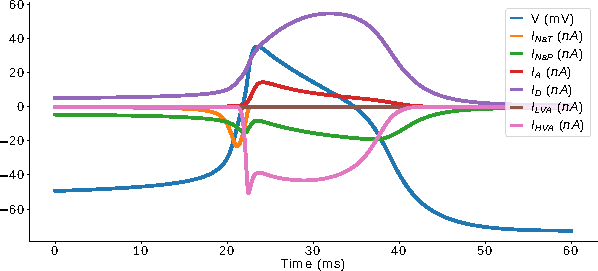
\includegraphics[width=\textwidth]{img/laser/cgc-model-simulation.pdf}
	\caption{Simulation of the CGC-model representing the voltage dynamics during an action potential and the corresponding ionic currents defined in the model ($I_{\textrm{NaP}}$,$I_{\textrm{NaT}}$, $I_{\textrm{A}}$, $I_{\textrm{D}}$, $I_{\textrm{LVA}}$,$I_{\textrm{HVA}}$). The units in the $y$-axis are specified in the legend.}
\end{figure}


\subsubsection{Temperature dependence description in the model}
\label{sec:model equations temperature}
To simulate the temperature dependency in the neuronal activity, a $Q_{10}$ factor was incorporated to every dynamical equation in the model (i.e., conductances and activation gates). $Q_{10}$ represents temperature sensitivity in each channel and it was included as a new factor as shown in Eqs. \ref{Q10_conductance} and \ref{Q10_gates}, with $i=Na_T,Na_P,A,D,LVA,HVA$ for Eq. \ref{Q10_conductance} and $i=h,r,a,b,n,d,e,f$ for Eq. \ref{Q10_gates}. The capacitance was also defined as temperature dependent ($C_T$) with a linear relation to the difference of temperature: 

\begin{equation}g_i(T)=\bar{g}_i{Q^i_{10}}^{\frac{T-T_0}{10}},
	\label{Q10_conductance}
\end{equation}
\begin{equation}\phi_i(T)=\bar{\phi}_i{Q^i_{10}}^{\frac{T-T_0}{10}},
	\label{Q10_gates}\end{equation}
\begin{equation}C_T=c_0 + c_0 \gamma(T-T_0).\end{equation}


where $\bar{g}_i$, $\bar{\phi}_i$, $c_0$ are the original values used in the model and $\gamma = 0.05$.

\subsection{Feeding CPG model}
\label{sec:CPG model}
The Vavoulis et al. description of the individual neurons considers a two-compartment model to represent the soma and the axon as  differentiated structures coupled by an axial resistance \cite{Vavoulis2007}. This separation of the soma and the axon is used to regulate the interaction between the fast and slow dynamics in the model. The slow dynamics are located the soma, whereas the fast dynamics are included in the axon compartment. This distributed formalism is represented in Fig. \ref{fig:CPG diagram 2 compartments}a., where each circle represents either soma or axon, containing the different ionic currents for each one. The description of the voltage dynamics is provided by equations (\ref{eq:soma}) and (\ref{eq:axon}) for soma and axon compartments, respectively: 

\begin{equation}
	\tau_m\frac{dV_S}{dt} = i_{inj} - i_{L,S} - i_X - i_{ec,S} - i_{syn} \\,
	\quad with \quad i_X = [i_{ACh},i_{NaL},i_T]
	\label{eq:soma}
\end{equation}

\begin{equation}
	\tau_m\frac{dV_A}{dt} = -i_{L,A} - i_{NaT} - i_K - i_{ec,A}
	\label{eq:axon}
\end{equation}


\begin{figure}
\centering
\begin{minipage}[t]{0.45\textwidth}
	\raggedright
	(a) \par
	\vspace{75pt}
	\includegraphics[width=\textwidth]{methods/invariants-model/figure1a.eps}
\end{minipage}\hfill
\begin{minipage}[t]{0.45\textwidth}
	\raggedright
	(b) \par
	\includegraphics[width=\textwidth]{methods/invariants-model/figure1b.eps}
\end{minipage}
	\caption{\textbf{Panel (a)}. Ionic channel distribution in the two-compartment description for the individual neurons in the Vavoulis et al. model \cite{Vavoulis2007} used in this study. At the soma: $I_{ACh}$, acetylcholine ionic channel; $I_{NaL}$, slowly inactivating sodium
		ionic channel;$I_T$, low-threshold calcium current; $I_{inj}$, injected current; $I_{L,S}$, leakage current in the soma; $I_{syn}$, synaptic current. At the axon: $I_{NaT}$, fast inactivating sodium current; $I_K$, delayed rectifier potassium current; $I_{L,A}$, leakage current in the axon. The electrical couplings are described as $I_{ec,S}=g_{ec}(V_S-V_A)$ and $I_{ec,A}=g_{ec}(V_A-V_S)$, respectively, being $g_{ec}$ the coupling conductance. The color for each $I_X$ current represents the CPG neuron that includes it at the soma,  N1M, N2v and N3t, respectively, as shown in panel (b). 
		%cambios
		\textbf{Panel (b)}. Connection scheme for the {\sl Lymnaea} feeding CPG circuit model. For details on the ionic channel current descriptions and associated parameters, see \cite{Vavoulis2007}. The colors indicating each neuron in the circuit match those in the representation of their corresponding somatic membrane potential traces throughout the paper. 
	}
	\label{fig:CPG diagram 2 compartments}
\end{figure}

\vspace{0.3in}

\noindent Here we follow the notation of~\cite{Vavoulis2007} where $\tau_m$ represents the time constant of the membrane (in ms) given by the ratio of the membrane capacitance (in nF) and the leakage conductance (in $\mu$S).  In equations \ref{eq:soma} and \ref{eq:axon}, $i$ variables (given in mV) are the product of the corresponding currents (in nA) times the passive input resistance given in M$\Omega$.
%, $i=I*R$, where  $R$ is given in M$\Omega$.

The soma compartment contains a slow current $I_X$ whose ionic nature depends on the specific CPG neuron described (see Fig.~\ref{fig:CPG diagram 2 compartments}a.). Thus, $I_X$  represents one channel, either $I_{ACh}$, $I_{NaL}$ or $I_{T}$, responsible of the specific slow dynamics associated with neurons N1M, N2v and N3t, respectively.  Along with the slow ionic channel and the leakage channel  $I_{L,S}$, the soma compartment also receives the synaptic current $I_{syn}$ and the injection current $I_{inj}$. All currents are explained in detail below.

On the other hand, fast channels are part of the axon compartment: a fast inactivating sodium current $I_{NaT}$ and a delayed rectifier potassium current $I_{K}$. These channels, along with the axon leakage channel  $I_{L,A}$ follow the definition in \cite{HODGKIN1952} model.

The model cells as described above are not endogenously bursters so to achieve bursting activity, a distinct constant value of  \(i_{inj}\) is applied to the cells. 

The CPG topology scheme is shown in Fig. \ref{fig:CPG diagram 2 compartments}, where the connections between neurons are represented by dashed or solid lines, depending on whether the connection is slow or fast, respectively, and filled or empty circles at their end denoting the direction and the effect on the postsynaptic neuron: excitation (empty circles) or inhibition (filled circles).
Individual neurons following the previous description are connected by graded synapses, defined by equations \ref{eq:syn1}-\ref{eq:syn2} \parencite{Vavoulis2007}. The differential point of a graded synapse is that it is dependent on voltage values and time, many synapses models used are just dependent on a trigger voltage value, that activates the synapse (see Figure \ref{fig:synapses-models example} ple of each type). This model of synapse allows dynamical adaptation of neurons in the circuit to maintain the rhythm despite the variability. \todo{discutir en el capítulo}

\begin{equation}
	i_{syn} = \sum_j \gamma_{syn,j} s_j (V_S - E_{syn,j})
	\label{eq:syn1}
\end{equation}

\begin{equation}
	\frac{ds_j}{dt} = \frac{r_{j}-s_j}{\tau_{syn,j}}
\end{equation}

\begin{equation}
	\frac{dr_j}{dt} = \frac{r_{\infty,j}-r_j}{\tau_{syn,j}}
\end{equation}

\begin{equation}
	r_{\infty,j}=\frac{1}{1+e^{(-40-V_{pre_{V_S}})/2.5}}
	\label{eq:syn2}
\end{equation}


\noindent where index $j$ runs over all presynaptic neurons and \(\gamma_{syn,j}, E_{syn,j},\tau_{syn},V_{pre_{V_S}}\) are the product of input resistance and maximal synaptic conductance, the synaptic reversal potential, the synaptic time constant and the presynaptic potential, respectively. 


\begin{figure}[h!]
	\centering
	\includegraphics[width=\linewidth]{methods/invariants-model/figure2.eps}
	\caption{Triphasic feeding rhythm as produced by the circuit CPG model described in Fig. \ref{fig:CPG diagram 2 compa}. In this simulation, $i_{inj}$ values applied to each neuron are 8.5, 6, 2 and 0 mV, respectively.}
	\label{fig:model simulation}
\end{figure}

The 3 inter-neurons described in this circuit have different waveform shapes, determined by their corresponding ionic channel and the axon connectivity, in Fig. \ref{fig:model simulation}  \todo{quitar marcos} there is an example of a simulation with all neurons in the circuit. First, N1M voltage characteristics are provided by an acetylcholine sensitive channel (\(i_{ACh} = 200 * p^3 * (V_S + 30)\)), which causes the gradual spiking frequency increase as well as the visible plateau, i.e., the slow wave is sustained before hyperpolarization. On the other hand, N2v has a slowly inactivating sodium channel (\(i_{NaL} = 2 * p^3 * q^3 * (V_S-55)\)), which causes the slow depolarization in this neuron. N2v neuron has a lower spiking frequency caused by the conductance value given for the axial $g_{ec}$ linking the two compartments, which is much lower in this cell. Finally, the N3t neuron has the particularity of a post inhibitory rebound, which generates an initial fast spiking followed by a decrease in the firing rate as the burst evolves. This latter property is caused by a low-threshold calcium channel (\( i_T = 3.27 * p^3 * q *(V_S-80)\)). SO neuron has no \(I_X\) channel (in contrast to N1M, N2v and N3t neurons) so its activity is the result of the combination of the common ionic channels in the axon and the soma.

 
\section{Neural data analysis}
Although models where implemented in $C++$ taking advantage of its computational speed, most analysis where performed in Python3, since it is a frequently used tool and libraries as Pandas are very effective for data analysis. 
Scripts are available at \todo{ add link to git. }

\section{CW-NIR laser}
The experimental results presented here were obtained using a continuous-wave (CW) NIR diode laser in single TEM00 operation and 830nm wavelenght output (Integrated Optics 0830L-13A-NI-PT-NF). \begin{wrapfigure}{l}{0.5\textwidth}
	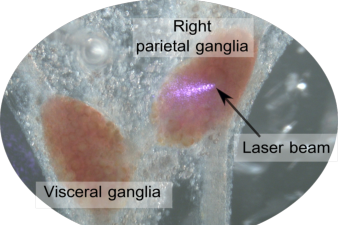
\includegraphics{img/laser/laser-beam.pdf}
	\caption{Illustration of the laser beam focused on a neuron in the right parietal ganglia.}
	\label{fig:laser beam}
\end{wrapfigure} 
The diode laser output was coupled to a single-mode optical fiber to efficiently guide the laser beam to the sample. To adapt the divergence of the laser beam to the fiber optic output, an aspherical lenses-collimator (Thorlabs, F280FC-850) was installed. An achromatic doublet with focal length f=50mm was used to focus the laser beam on the sample (Thorlabs AC127-050-B-ML). The experiments were performed with a laser output power of $\sim$ 90 mW and a power density over the sample of 146 W/cm². The grazing incidence of the laser beam on the sample created a quasi-elliptical spot, with a minor axis of approximately 34{\textmu}m, as shown in Fig. \ref{fig:laser beam}.



The laser was attached to a micro-manipulator (Siskiyou MX160), allowing micrometer precision of the beam placement over the neuron and optimization of the beam focus. The focusing was performed using a binocular microscope (Nikon SMZ-1500) coupled to a CCD camera (XCAM1080PHA, ToupTek Photonics, Zhejiang, China).


\section{Temperature estimation for analyzing laser neuromodulation}
\label{sec:temperature-estimation}
To estimate the CW-NIR laser induced temperature change, we used the open-pipette method employed in previous experimental studies to measure the temperature variation during the illumination \parencite{li_temporal_2013, rabbitt_heat_2016,brown_thermal_2020, brown_response_2021}. We calibrated the resistance and temperature relation using a thermistor (EPCOS, 10$k\Omega$) to measure the temperature in the preparation solution in the range from 23ºC to 29ºC. We used two protocols:  injecting a constant current to calculate the resistance change from the voltage recording, and injecting pulses of a specific current value. From the resulting recording slope of the linear regression, we computed the conversion from voltage to temperature. For the estimation of the temperature change during the laser stimulation, we measured the voltage change during short intervals of laser illumination and the temperature value at its saturation plateau. This estimation is represented in Fig. \ref{fig:temperature estimation}.



\begin{figure}[htb!]
	\centering
	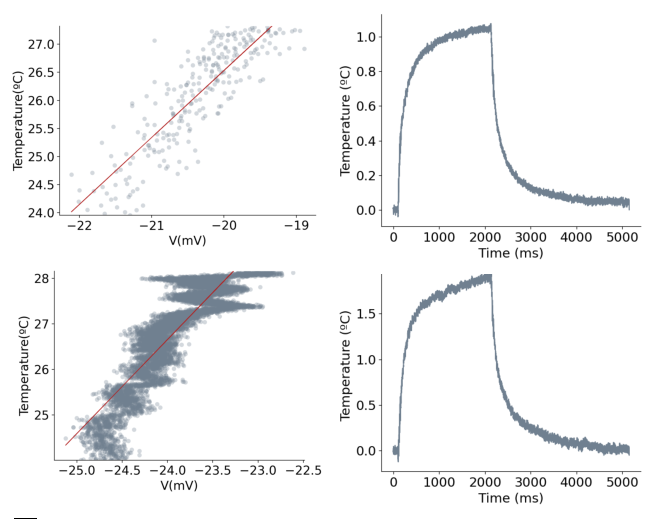
\includegraphics[width=0.8\textwidth]{img/laser/temperature_estimation.pdf}
	\caption{Open-pipette temperature estimation method. Each row in the panel represents pulsed and continuous current delivery for the estimation, respectively. For both examples: left column, temperature and voltage relation. Right column filtered mean of voltage recordings from short illumination intervals in the pipette. }
	\label{fig:temperature estimation}
\end{figure}


	%%!TEX root = ../_thesis.tex
\chapter{Sequential constrains in CPG circuits: Dynamical invariants}
\label{c-invariants}
\section{Introduction}
%Paper model
Although often disregarded in many experimental and theoretical studies, neural sequences are key elements of brain activity which, in many cases, have a direct relationship to behavior \parencite{hahnloser_ultra-sparse_2002,venaille_synchronization_2005,buzsaki_space_2018,rabinovich_discrete_2018,paton_neural_2018,elices_robust_2019}.
% \parencite{hahnloser_ultra-sparse_2002,venaille_synchronization_2005,hb10,buzsaki_space_2018,rabinovich_discrete_2018,paton_neural_2018,elices_robust_2019}.
%This neural sequences have been observed experimental and theoretically, and are considered to be the ones carrying information in the neural system, playing an important role in the function these systems generate. 
The study of neural sequences involves the assessment of time references, time intervals and the associated temporal structure of individual neurons, groups of neurons or large neural ensembles, which typically hinder their characterization due to experimental limitations. In this context, Central Pattern Generators (CPGs) are adequate neural circuits to study the generation and coordination of neural sequences. 
%Hence, when studying neural activity it is not only important the response a single cell might produce (measured in form of ISI analysis, return maps, etc.) but the interaction it has in a whole circuit. It is due to the interaction between different cells and the effect of the synapses they are affected by, that some function in a living element is generated. Indeed, many motor rhythmic activity have their origin in closed cell circuits. This is the case of Central Pattern Generators (CPGs).

CPGs are neural structures capable of generating rhythmic activity that involves robust motor sequences in a highly autonomous manner \parencite{hartline_mottor_1976,selverston_reliable_2000,marder_central_2001}. This kind of circuits are found in many different organisms including humans \parencite{dimitrijevic_evidence_1998,pavlidis_neonatal_2016, arichi_localization_2017}. CPG neurons have rich intrinsic dynamics and their connections form non-open circuit topologies in which all members of the circuit receive information from at least another member in the ensemble \cite{selverston_reliable_2000,huerta_topology_2001}. This favors rhythm coordination through closed-loop computation and endows CPGs with the ability to produce robust yet flexible rhythms where intervals building the sequences can be adapted in different behavioral contexts \parencite{elices_robust_2019}. %These intervals building the sequences cycle-by-clycle, are defined as different temporal events in each neuron, such as burst duration. 
In Fig. \ref{fig:sequences_in_cpgs} there is an example of the robust sequential generation of bursts in a CPG. 

\begin{figure}[htb!]
	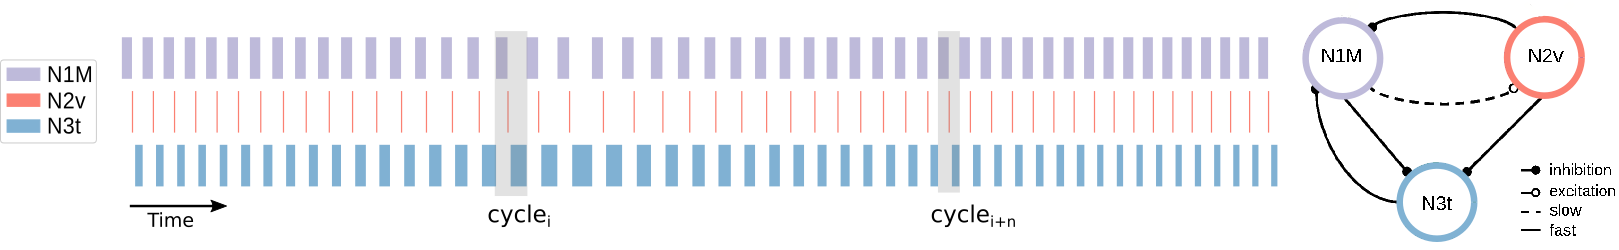
\includegraphics[width=\textwidth]{img/invariants/variability/sequences_in_cpgs.png}
	\caption{Example of robust sequential bursting dynamics in CPGs. Representation of burst duration in 3 neurons in a CPG model, the sequential activation of the three neurons conform cycles (transparent grey boxes in the sequence). The connections between the three neurons are represented in the diagram on the right side of the panel.}
	\label{fig:sequences_in_cpgs}
\end{figure}

The sequence of intervals underlying CPG rhythms present variability in the duration of each cell activation/inactivation, which has been identified in different nervous systems, e.g. see \cite{reyes_artificial_2008,Elliott1991,martinez_short-term_2019}. Consequently to the study of variability in cycle-by-cycle sequences, we have recently found sequential dynamical invariants in the form of robust linear relationships between specific sequence intervals and the period in the pyloric CPG of shore crabs (\textit{Carcinus maenas}) \parencite{elices_robust_2019}. Dynamical invariants represent constraints of particular sequence intervals in relation to different intervals in the same cycle as the instantaneous duration of the period and build rules for the overall flexibility of the rhythm. It is important to note that not all intervals composing the sequence display such constraints. The presence of invariants in the crustacean pyloric CPG are observed in all control conditions as well as in experiments under the effect of ethanol, which induces irregular rhythms \parencite{elices_robust_2019}. 

%\red{Moreover, different experimental cases are described in this study, including recordings with ethanol and PTX application. The invariants were found to be present even under those circumstances which alter the neurons activity and their variability}.

%settle an evidence in the strong relation between the sequential activation and the period duration, highlighting the importance of the temporal variability which is always present in the same intervals.

While the existence of phase maintenance and linear relationships between rhythm intervals and the period have been discussed before in convenient animal models, e.g. \cite{grillner_generation_1976,hooper_phase_1997,vavoulis_dynamic_2007}, detailed characterization of cycle-by-cycle variability to understand the existence of these relationships and the corresponding analysis of the universality of robust dynamical invariants are pending in both computational models and living recordings. The observation of this restriction in other animal models, can also support the association of these temporal restrictions to a functional, biological meaning.

During this chapter we will characterized the sequence interval variability in a model of the \textit{L. stagnalis} feeding CPG inducing variability with a ramp current injection, we will also address the issue of variability in models to study this kind of phenomena, and explore and discuss the presence of sequential dynamical invariants in living intracellular recordings as well as their possible functional role by inducing the activity from different methods but also from a practical approach in robotics. 

%In particular, a thorough analysis of interval variability in CPG models and their use in understanding the generation of dynamical invariants within specific time intervals have not been addressed. The main difficulty to study the functional balance between flexibility and robustness in sequences generated by theoretical models is the lack of variability both in the intrinsic and network dynamics. In this paper, we report the characterization of sequence interval variability in a model of the \textit{Lymnaea} feeding CPG.  By using ramp current injection protocols, it is possible to induce variability in the collective activity of the neurons of this CPG model. This enables the study of the evoked variability of the intervals conforming each cycle following the same interval definitions from \cite{elices_robust_2019}, as well as the conceivable presence of dynamical invariants, which we address here. 


\section{Methods}

\subsection{Time references, intervals and CPG sequence}
\label{subsec:intervals}
The variability study addressed in this chapter is based on the characterization of cycle-by-cycle intervals in the rhythm produced by the model CPG.
In our analysis of variability, we assess the presence of linear relationships between the intervals that build the sequence and the cycle-by-cycle period to characterize and unveil similar dynamical invariants as those found in the stomatogastric CPG \cite{elices_robust_2019}. 
The intervals here analyzed can be measured for any three neurons following a robust triphasic rhythm. In this paper N1, N2 and N3 represent the feeding CPG phases, represented in the model by interneurons N1M, N2v and N3t, respectively and in the experimental data by different combinations of moto- and interneurons.

\begin{figure}[hbt!]
	\centering
	\begin{minipage}{\textwidth}
		\centering
		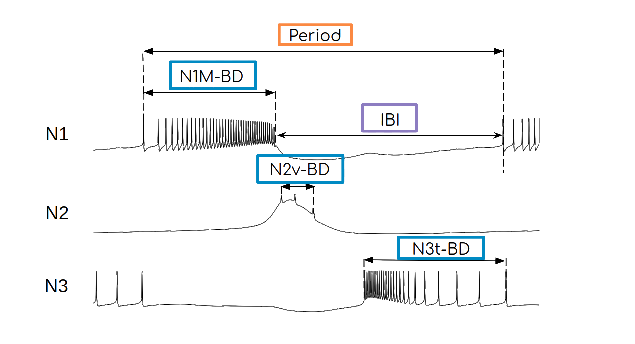
\includegraphics[width=0.8\textwidth]{img/methods-paper-modelo/figure4a.eps} 
		\label{fig:intervals_bd}
	\end{minipage}
	% \hfill
	
	\vspace{1cm}
	\begin{minipage}[t]{\textwidth}
		\centering
		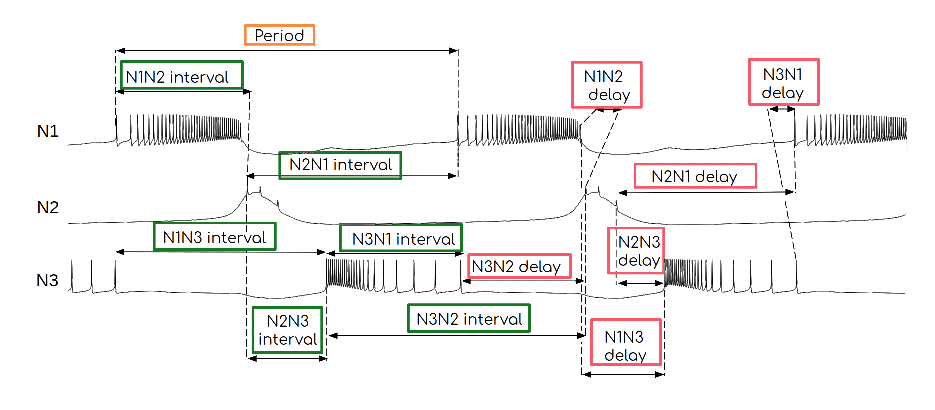
\includegraphics[width=\textwidth]{img/methods-paper-modelo/figure4b.eps} 
		\label{fig:intervals_der}
	\end{minipage}
	
	\caption{\textbf{Panel A}. Individual neuron sequence interval definitions. Each BD label represents the burst duration, defined as the time interval from the first spike to the last spike in the neuron's burst. Period was measured as the interval from the first spike of N1 burst to the first spike of the next N1 burst, covering three phases %(N1M,N2v, N3t) 
		in relation to the activity of the other neurons. IBI represents the interburst interval, defined as the time from the last spike of a neuron's burst to the first one of the next burst in the same neuron.
		\textbf{Panel B}. Definition of intervals involving pairs of neurons. NXNY interval represents interval from NX start to NY start. NXNY delay represents interval from NX end to NY start. Period was measured from N1 start to N1 start, covering the three phases of the CPG rhythm.
	}
	
	\label{fig:intervals}
\end{figure}


This is illustrated in Fig. \ref{fig:intervals}, where single neuron intervals and intervals defined between neurons are depicted and the definition of each interval is as follows:
\begin{enumerate}
	\item \textbf{Burst Duration (BD)}, measured as the time interval between the first and the last spike of the burst (start to end in the trace of a given neuron).
	\item \textbf{Inter Burst Interval (IBI)}, characterized as the difference between the last spike of a burst and the first one of the next one (end to start in the trace of a given neuron).
	\item \textbf{Period}, which envelops the bursts from the three neurons, measured as the distance between the first spike of one burst in a neuron and the first spike of the next one on that neuron (start to start).
	\item \textbf{NeuronX-NeuronY interval}, this interval is measured from the start of the burst of neuron X to the start of the burst of neuron Y (start X to start Y).
	\item \textbf{NeuronX-NeuronY delay}, being the time lapse between the burst end of a neuron X and the burst beginning of neuron Y. (end X to start Y).
\end{enumerate}

\subsection{Inducing variability in the model by current injection}
\label{subsec:inj protocol}
The spiking-bursting activity of the model CPG neurons can be modulated by using an additional current injection on each cell, implemented in the \(i_{inj}\) term of equation (\ref{eq:soma}), as performed in many experimental protocols. Depending on the current value applied, the corresponding neuron dynamics changes. While for N2v a change in this injection corresponds to a change in burst frequency (i.e. the number of bursts increases/decreases), for the rest of the neurons in the model a change in \(i_{inj}\) affects burst duration for N3t and SO, and the length of the depolarization phase in N1M.


\begin{figure}[hbt!]
	\centering
	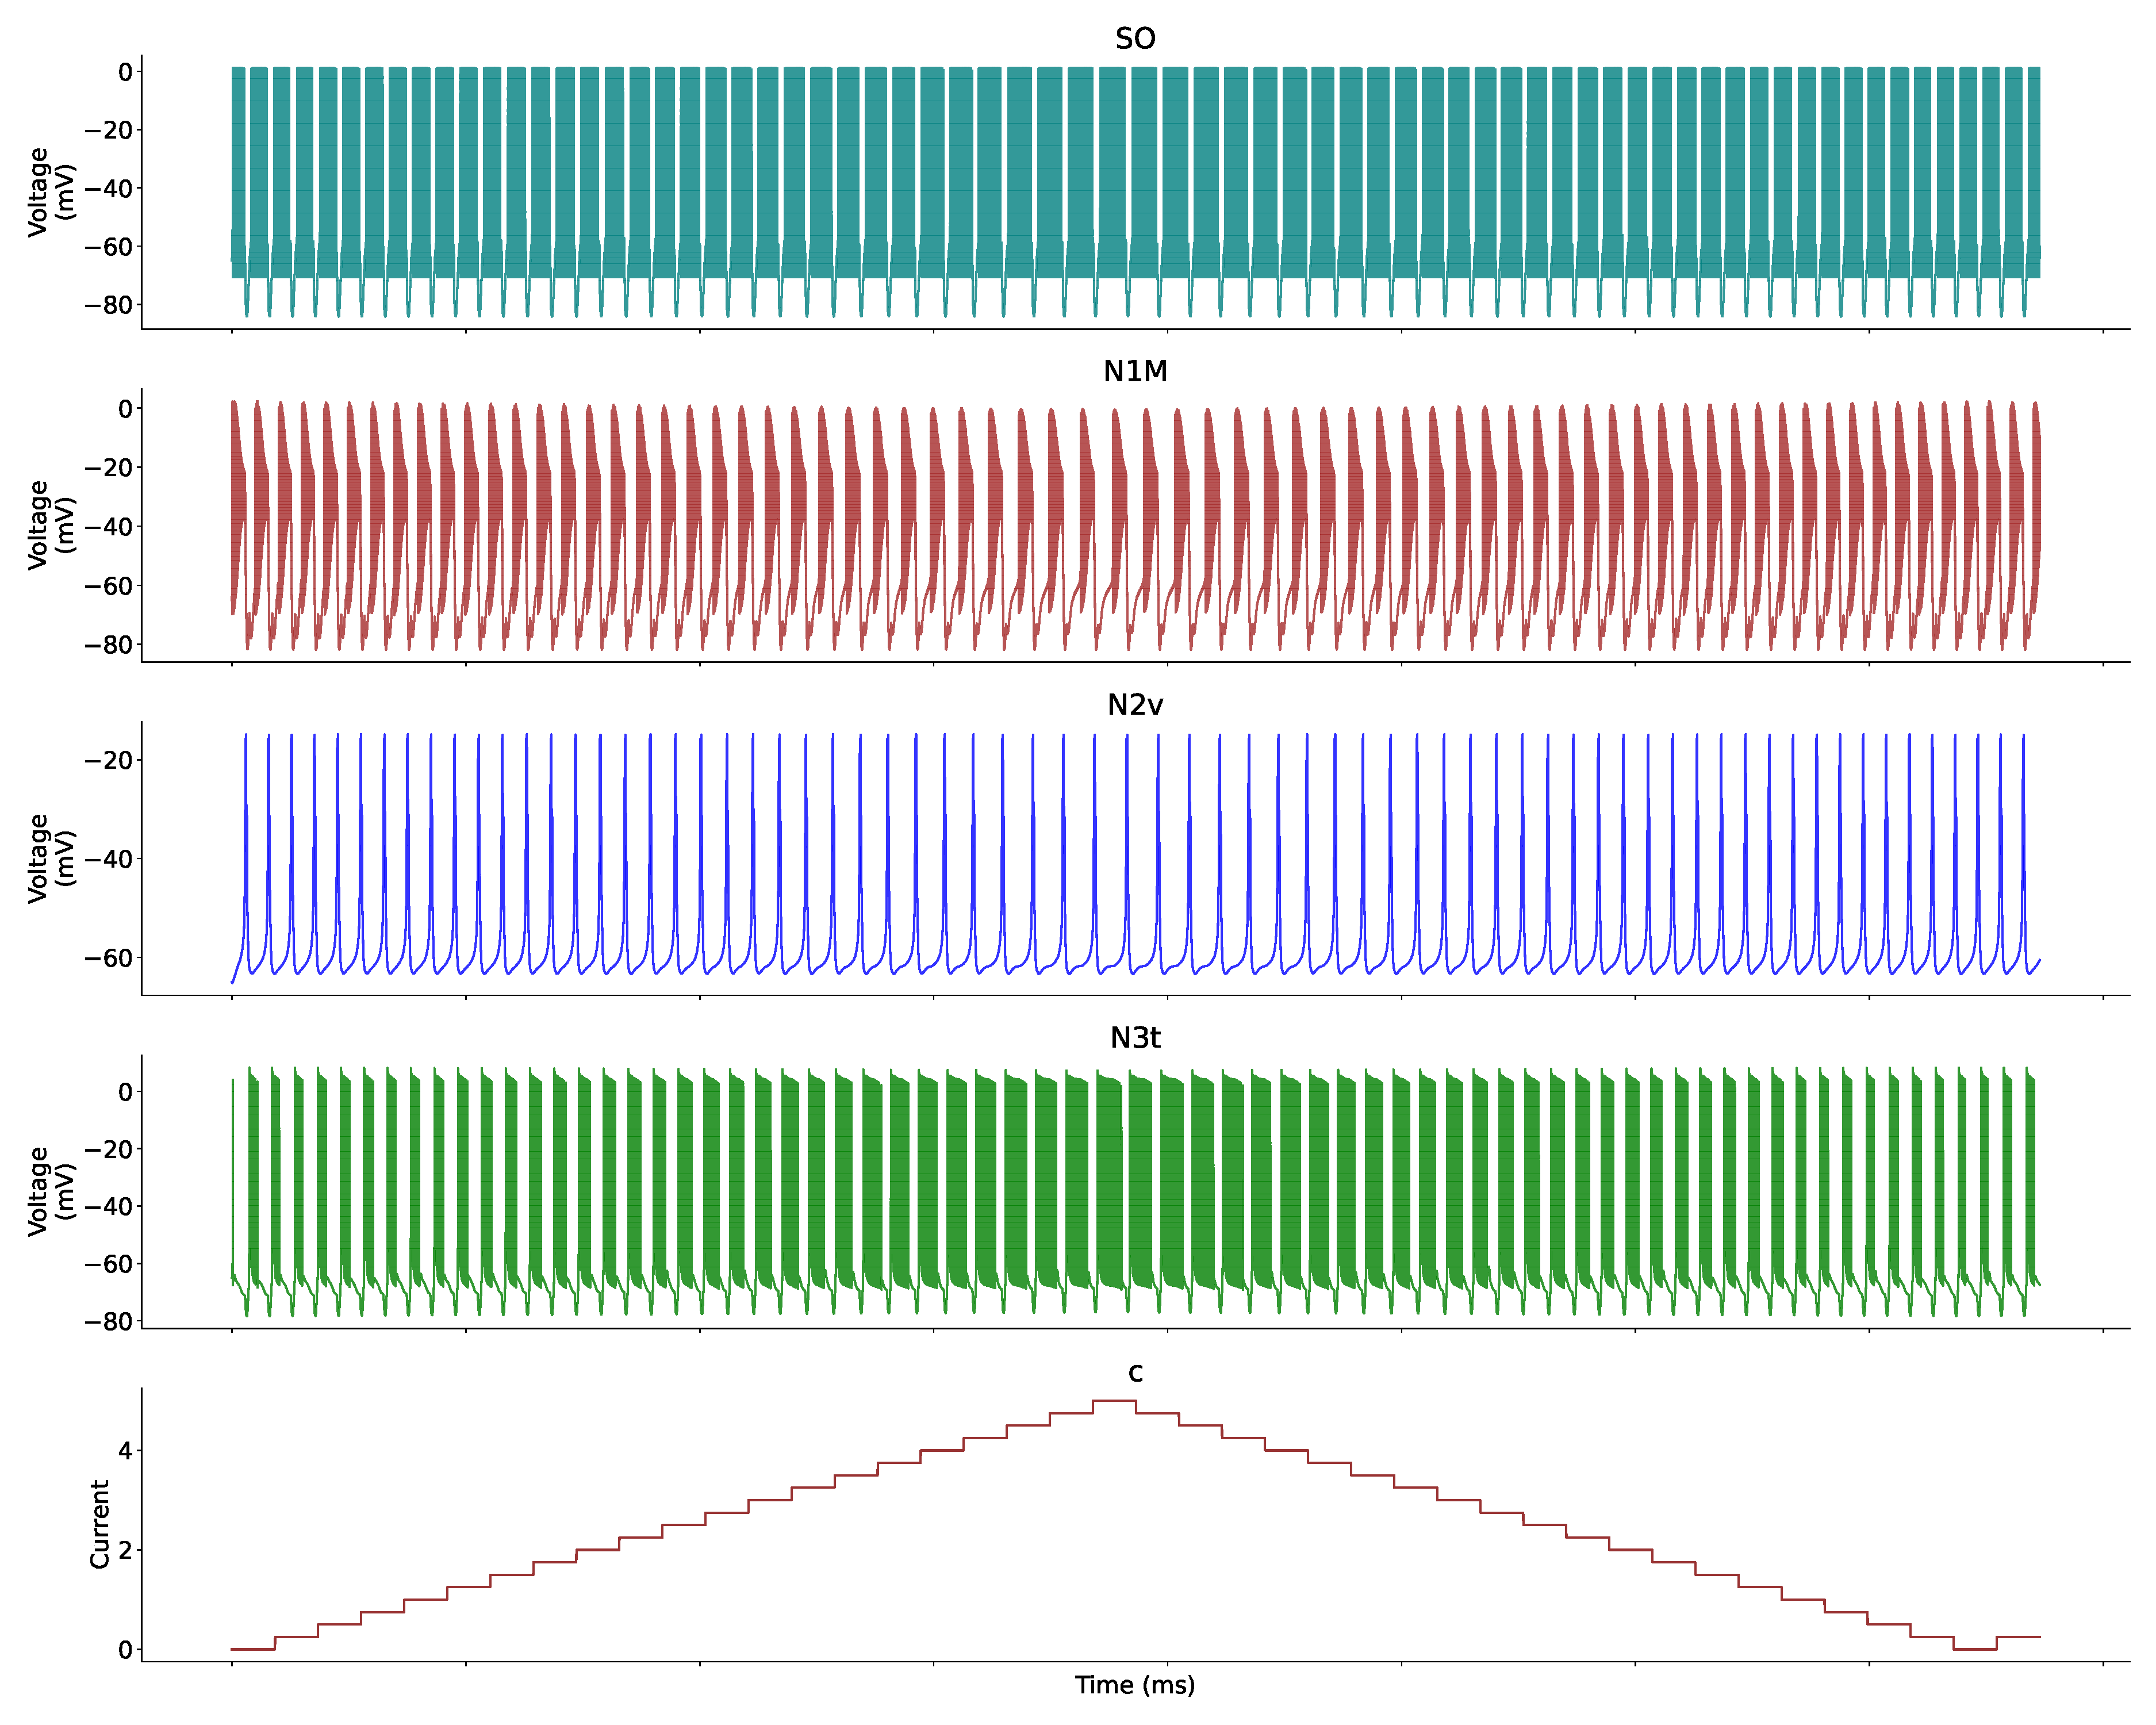
\includegraphics[width=\textwidth]{img/methods-paper-modelo/circuit_w_current.pdf}
	\caption{Illustration of the CPG activity when a current ramp \(i_{inj}\) is applied to N3t. Variability in the sequence intervals was induced by applying two consecutive ramps as the one shown in this figure into different cells.  }
	\label{fig:complete ramp example}
\end{figure}

Whilst the single neuron model descriptions have no intrinsic variability, the effect produced by the modulation of the injected current in each neuron induces variability into the circuit, which allows characterizing the sequence intervals and the period, the associated robustness of the rhythm and the presence of dynamical invariants. Such stimulation has been used previously in the living circuit, as reported by \cite{Elliott1991}. The authors of this work showed that it is possible to activate the feeding CPG with variability caused by current injection into individual cells in the circuit. CPG rhythms obtained under this type of stimulation differ depending on which neuron is being stimulated. To induce variability in the model we used a ramp protocol resulting in circuit time-interval variations as in Fig. \ref{fig:complete ramp example}.

% Even though this CPG model do not present intrinsic variability, thanks to the current \(i_{inj}\), variability is induced into the model, effectively changing burst duration. This current injection has also been used in Lymnaea preparation in living elements, stimulating N1M and SO, obtaining rhythm. Neural sequences obtained after the stimulation differ one another depending on which neuron is being stimulated. 


By varying the current injected into N1M, its burst duration is kept nearly constant, but its depolarization phase before the spiking activity begins becomes longer. Since N3t is the neuron fitting in the sequence in that phase (see Fig. \ref{fig:model simulation}), it also increases its burst duration, being the most variable one in the CPG rhythm. 

When value \(i_{inj}\) is increased on neuron SO, its burst duration becomes longer. Since SO has a modulator effect over N3t and N1M, it also alters the burst duration of these two neurons.

Neuron N3t also shows variable burst duration when an evolving current is injected. When \(i_{inj}\) value on N3t is larger, its burst duration increases, elongating the N1M depolarization phase.  

Finally, when current is applied to N2v the effect on its burst duration or the burst duration of the rest of the neurons is rather small. However, \(i_{inj}\) % current 
modulates N2v burst frequency through the hyperpolarization phase. 

%cambios
Therefore, we used a current ramp protocol to induce variability in the CPG model defined as follows: a ramp variable $c$, which controlled the current injection value ($i_{inj}=c$) on the neuron being stimulated, was increased from a minimum to a maximum value, and then decreased back to the initial value. This was repeated twice in each simulation. The ramp variable was modified with a fixed step value every 4.6 seconds (the approximate duration of two N3t bursts). The minimum and maximum $c$ values were different in each cell and were tuned to generate realistic spiking-bursting behavior. All parameters used for the simulation analyses reported in this paper are summarized in Table \ref{table:inj values}.

\begin{table}[h!]
\centering
\begin{tabular}{c|cccc|c|ccc|}
\multirow{2}{*}{\textbf{\begin{tabular}[c]{@{}c@{}}Neuron\\ stimulated\end{tabular}}} & \multicolumn{4}{c|}{\textbf{\(i_{inj}\) value}}                 & \multirow{6}{*}{} & \multicolumn{3}{c|}{\textbf{Ramp values ($c$)}}   \\ \cline{2-5} \cline{7-9} 
                                                                                      & \textbf{SO} & \textbf{N1M} & \textbf{N2v} & \textbf{N3t} &                   & \textbf{Min} & \textbf{Max} & \textbf{Step} \\ \cline{1-5} \cline{7-9} 
\textbf{N1M}                                                                          & 8.5         & $c$            & 2            & 0            &                   & 0            & 10.5         & 0.5           \\ \cline{1-5} \cline{7-9} 
\textbf{N3t}                                                                          & 9           & 10           & 1            & $c$            &                   & 0            & 5            & 0.25          \\ \cline{1-5} \cline{7-9} 
\textbf{SO}                                                                           & $c$           & 10           & 1            & 4            &                   & 8.2          & 13           & 0.25          \\ \cline{1-5} \cline{7-9} 
\end{tabular}
\caption{List of \(i_{inj}\) values that yield realistic bursting rhythms for each neuron in the model CPG used in the stimulation protocols reported in this paper. The left section of the table displays the \(i_{inj}\) values applied to each neuron (columns) during each simulation condition (rows). Ramp values on the right section refer to the minimum and maximum values of the ramp variable $c$ in each simulation, increasing \(i_{inj}\) in the specified step every 4.6 seconds (the approximate duration of two N3t burst) to induce variability.} \label{table:inj values}
\end{table}

Simulations of \cite{vavoulis_computational_2007} model were implemented in C++. The code of the feeding CPG model implementation is available at \href{github.com/GNB-UAM/CPG-feeding-Lymnaea}{https://github.com/GNB-UAM/CPG-feeding-Lymnaea}. This model was also included in Neun library in a Github repository \href{github.com/GNB-UAM/Neun}{https://github.com/GNB-UAM/Neun}. Each simulation had the duration of two consecutive cycles of up and down ramps as the one shown in Fig. \ref{fig:complete ramp example} using the parameters described in Table \ref{table:inj values}. The number of bursts in each simulation was approximately 140 (this number slightly depends on the neuron stimulated). Parameter values such as reversal potentials and synaptic conductances were the same ones specified in \cite{Vavoulis2007}.


% \subsection{Model simulation specifications and statistical analysis}\todo{añadir en métodos generales o ampliarlo también a experimental}



\subsection{Experimental recordings and stimulation}
The experimental recordings analyzed in section \ref{sec:experimental sussex} were performed by Michael Crossley, University of Sussex, and kindly provided for this work. 

Each recording had at least 5 microelectrodes, which allowed to characterize the rhythm based on combinations of different neuron's activity. There are cases of experiments in that section:
\begin{itemize}
	\item Spontaneous activity: After the isolation of the CNS, the electrodes impailed in the neuron recorded the spontaneous activity in the CPG, with no further stimulation.
	\item Nerve electrical stimulation: For the activation of the rhythm it is possible to stimulate the median lip nerve (MLN). The data analyzed there was stimulated by a 4V stimulous at 1Hz. 
	\item Neuron electrical stimulation: To modulate the CPG rhythm, SO and CV1a neurons where stimulated (in different experiments) by injecting a constant depolarizing current.
\end{itemize}

%To define each phase, we used different neurons and bursting references, depending on the ones available on the circuit, following intervals definition in table \ref{table:cpg ref intervals}.
%
%For each recording each phase was defined as follows:
%
%\paragraph{Spontaneous Activity Example 1}
%N1 phase was analyzed from B1 activity (bursting and depolarization); N2 phase was analyzed from B5 hyperpolarization, which has a strong inhibition from N2v; N3 phase was analyzed from the bursting activity of B8, that replicates the N3t duration. 
%
%\paragraph{Spontaneous Activity Example 2}
%N1 phase was analyzed from B1 activity (bursting and depolarization); N2 phase was analyzed from B1 hyperpolarization, which has a strong inhibition from N2v; N3 phase was analyzed from the bursting activity of B8, that replicates the N3t duration. 
%Since the reference for N2 here coincides with N1 reference, we display here only the intervals corresponding to N1 and N3 phases, since the intervals that correspond to 3 phases, such as N1-N2 delay or N2-N3 delay, either are already represented in the defined intervals or have a duration close to 0 ms.
%
%\paragraph{Spontaneous Activity Example 3}
%N1 phase was analyzed from B1 activity (bursting and depolarization); N2 phase was analyzed from B5 hyperpolarization, which has a strong inhibition from N2v; N3 phase was analyzed from the bursting activity of B8, that replicates the N3t duration. 
%
%\paragraph{Spontaneous Activity SO modulation}
%N1 phase was analyzed from B1 activity (bursting and depolarization); N2 phase was analyzed from B5 hyperpolarization, which has a strong inhibition from N2v; N3 phase was analyzed from the bursting activity of B8, that replicates the N3t duration. 




\subsection{Models with chaotic activity}

\subsubsection{LP model by \cite{nowotny_probing_2008}}

The membrane potential of axon and soma compartment, $V_{\text{axon}}$ and $V_{\text{soma}}$ respectively, are described by

\begin{equation}
	\frac{dV_{\text{axon}}}{dt} = \frac{1}{C_a} \left( -I_{\text{Na}} - I_{\text{Kd}} - I_M - I_{\text{leak,a}} + I_{VV} \right)
\end{equation}

\begin{equation}
	\frac{dV_{\text{soma}}}{dt} = \frac{1}{C_s} \left( -I_{\text{Ca}} - I_{\text{KCa}} - I_A - I_h - I_{\text{leak,s}} - I_{VV} + I_{\text{scale}} (I_{\text{DC}} - I_{\text{offset}} + I_{\text{syn}} \right))
\end{equation}

$I_{\text{offset}} = 2 \, \text{nA}$ stems from the residual coupling at the end of the parameter estimation procedure which introduces a current bias due to differences in baseline voltage of data and model (on top of $V_{\text{shift}}$). $I_{\text{syn}}$ denotes the total incoming synaptic current. All ionic currents except for the ones mentioned explicitly below are given by

\begin{equation}
	I_x = g_x m^p h^q (V - V_x)
\end{equation}

where $g_x$ is the maximal conductance of the current, $V$ is the membrane potential of either the axon compartment ($I_{\text{Na}}$, $I_{\text{Kd}}$, and $I_M$) or the soma compartment (all other currents), and $V_x$ is the reversal potential of the current. The activation and inactivation variables are governed by

%\begin{equation}
%	\frac{dm}{dt} = \alpha_m (1 - m) - \beta_m m
%\end{equation}
%
%\begin{equation}
%	\frac{dh}{dt} = \alpha_h (1 - h) - \beta_h h
%\end{equation}
%
%for $I_{\text{Na}}$ and $I_{\text{Kd}}$, and
%
%\begin{equation}
%	\frac{dm_x}{dt} = \frac{m_{\infty,x}(V) - m_x}{\tau_{m_x}}
%\end{equation}

\subsubsection{Non chaotic model \cite{ghigliazza_minimal_2004}}
\todo{revisar}
The Ghigliazza and Holmes model for motoneurons is described by the following equations:

1. The membrane potential dynamics of a neuron is given by:

\begin{equation}
	C_m \frac{dV}{dt} = -\sum I_x + I_{\text{syn}}
\end{equation}

where \( C_m \) is the membrane capacitance, \( V \) is the membrane potential, \( I_x \) are the various ionic currents, and \( I_{\text{syn}} \) is the synaptic current.

2. The ionic currents \( I_x \) are typically given by:

\begin{equation}
	I_x = g_x m^p h^q (V - V_x)
\end{equation}

where \( g_x \) is the maximal conductance, \( m \) and \( h \) are the activation and inactivation variables, \( p \) and \( q \) are the respective powers, and \( V_x \) is the reversal potential of the current.

3. The gating variables \( m \) and \( h \) are governed by first-order kinetics:

\begin{equation}
	\frac{dm}{dt} = \alpha_m (1 - m) - \beta_m m
\end{equation}

\begin{equation}
	\frac{dh}{dt} = \alpha_h (1 - h) - \beta_h h
\end{equation}

where \( \alpha_m \), \( \beta_m \), \( \alpha_h \), and \( \beta_h \) are voltage-dependent rate constants.

4. For a central pattern generator (CPG), the model includes a set of coupled differential equations to describe the rhythmic activity:

\begin{equation}
	\frac{d\phi_i}{dt} = \omega_i + \sum_j K_{ij} \sin(\phi_j - \phi_i - \psi_{ij})
\end{equation}

where \( \phi_i \) is the phase of the \( i \)-th oscillator, \( \omega_i \) is the intrinsic frequency, \( K_{ij} \) is the coupling strength between oscillators \( i \) and \( j \), and \( \psi_{ij} \) is the phase shift.



\subsection{Hybrot structure}

We have designed and implemented a FLC-Hybrot, a hybrot controlled by the neural activity of a living and functional pyloric CPG, to validate the importance of the balance between robustness and flexibility in this circuit, as provided by cycle-by-cycle dynamical invariants present in its dynamics \cite{Elices2019}. With this idea in mind we built an hexapod robot whose legs performed oscillatory motions to move forward. The period and amplitude of these oscillations were determined by the sequential cycle-by-cycle activity of the CPG neurons. At the same time, the hybrot included a light sensor and sent feedback information regarding the light conditions around it back to the neural circuit in the form of an electrical current. These stimuli modified the behaviour of the cells, resulting in a change of the hybrot locomotion, preserving always the required motor coordination, and therefore forming a real-time closed-loop interaction among living and electronic components (Figure \ref{fig:robot_results_summary}). The goal of the FLC-Hybrot is to demonstrate that a dynamical principle of the functional living circuit can be used to coordinate the locomotion with sensory feedback from the robot. In our case, we use the presence of dynamical invariants in the form of robust relationships between the time intervals that build the cycle-by-cycle activity of the CPG, which are sustained under any circumstance even when there are external inputs to the circuit, to modulate the behavior of the robot. \todo{copia pega de paper robot adaptar}

\begin{figure}[h!]
	\begin{center}
		% \includegraphics[width=\linewidth]{images/robot/robot_results_summary}
		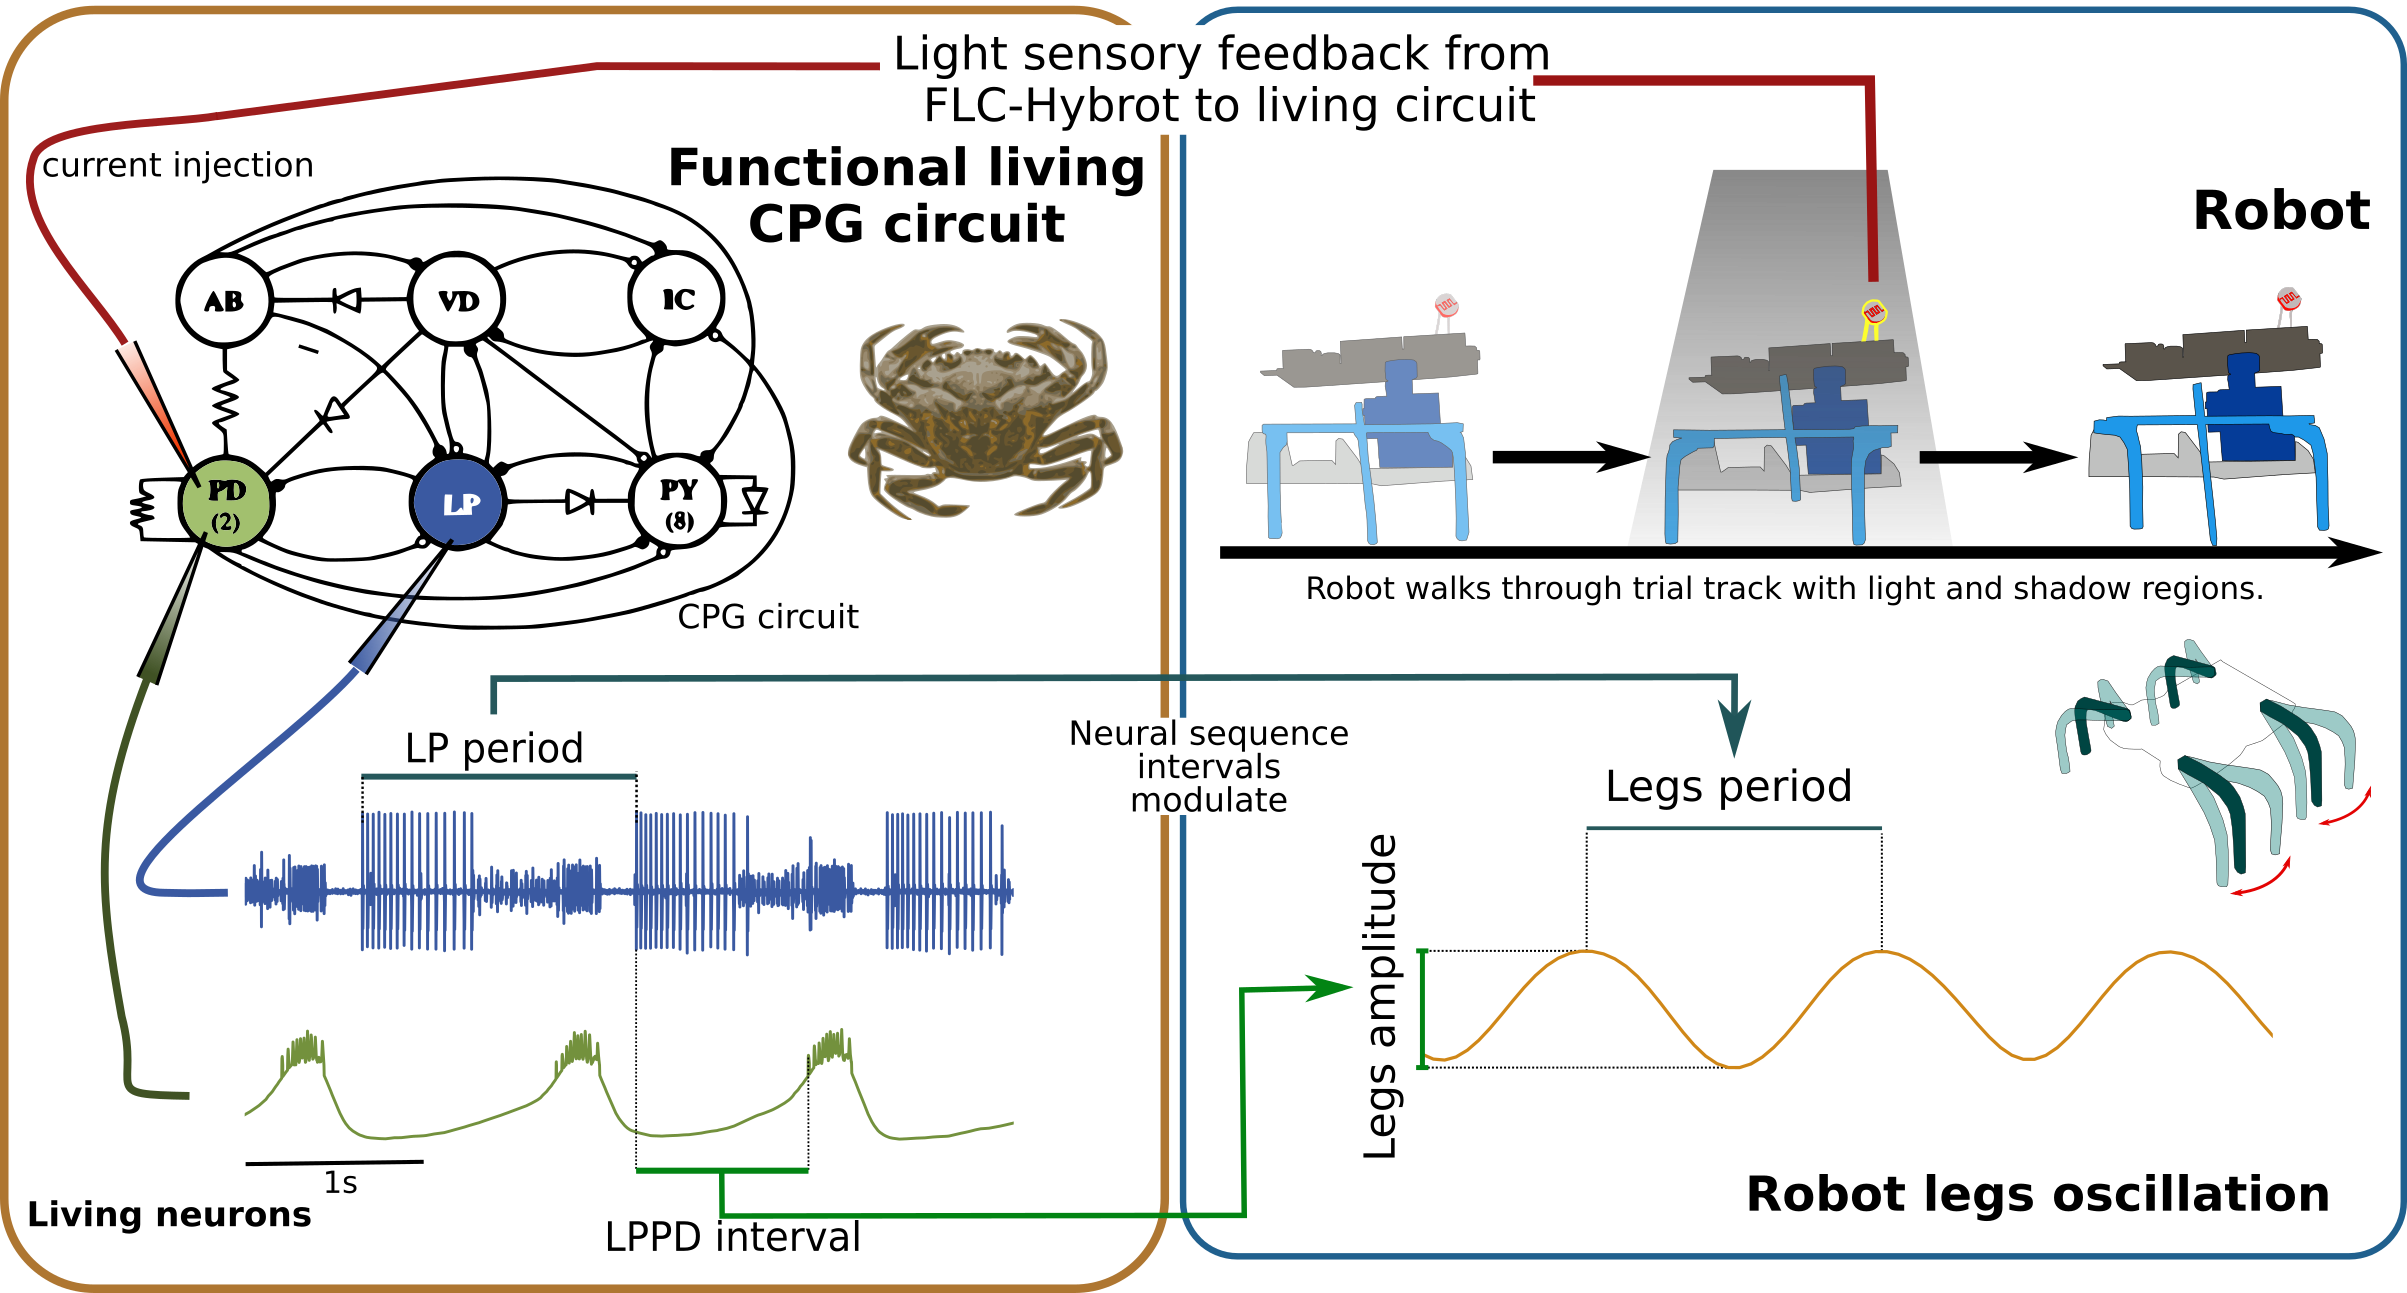
\includegraphics[width=\linewidth]{img/invariants/robot/Figure1_experiment_design_v1.png}
	\end{center}
	\caption{Representation of the FLC-Hybrot paradigm design. Neural dynamics from a functional living CPG circuit are recorded online and used to coordinate the robot movement in real-time. Activity from the PD neuron is recorded intracellularly (green trace), while the LP bursts are extracted from the nerve's extracellular signal (blue trace). This robot walks through a trial track with interspersed light and shadow regions. When the robot's light sensor detects that it is located under a shadow, it sends feedback current to the living circuit. CPG dynamics change as a reaction to the injected current, thus modifying the robotic locomotion. The following video shows an example of this experiment \url{https://youtu.be/ny2dJGbG8lo}.}
	\label{fig:robot_results_summary}
\end{figure}





\section{Sequential dynamical invariants in computational models}
\label{c-invariants-model}
In this section we will investigate the cycle-by-cycle sequential restrictions found in \cite{elices_robust_2019} in a computational model, the detailed reproduction of the activity allows to study in detail the mechanisms associated to the circuit and the time-interals relations. We used the feeding CPG model description of \cite{vavoulis_dynamic_2007}, which even though it does not have a chaotic mode, the model is flexible enough to adapt the variability of one of the neurons. Following the current injection protocol defined in section \ref{subsec:inj protocol}, N1M, N3t and SO neurons in the model were stimulated for our analysis of the sequence interval variability. Using this induced variability we were able to explore the presence of sequential dynamical invariants under different scenarios. The effect on injecting a current ramp on N2v is not reported here since it leads to lower variability than the other cases. In all simulations, we could test the robustness of the rhythm while inducing the external perturbation that evoked variability in the search for dynamical invariants. The results summarized and adapted for this section were published in \cite{garrido-pena_characterization_2021}.

First we saw in the simulations is that the model of the feeding CPG faithfully reproduces the activity of the main neurons involved in the generation of its triphasic rhythm \parencite{Vavoulis2007}. This includes their waveforms and the relationships between the cycle period and the duration of several intervals reported in \parencite{Elliott1991}. Note that, since there was not a description of a chaotic mode, all the rhythms explored here were analyzed from induced stimulation, not by simulating spontaneous activity. This was a restriction when exploring spontaneous activity, since the circuit needed to be altered by one of the neurons, simulating a extended experimental protocol, but still altering the circuit in a predefined way. Also, other phenomena reported in the pyloric CPG experimental work, were there was a "reset" in the inter-cycle dynamics of the dynamical invariants, could not be explored in this model, since the ramp value was progressive (see Apendix Fig. \ref{fig:N1M stimulation pairplot reset} for a representation of this non-reset output). All this will be illustrated in the following Section \ref{sec:experimental sussex} with experimental recordings and other options to reproduce the functional variability will be discussed in Sec. \ref{sec:model variability}

\subsection{N1M driven variability}
\label{subsec:n1m driven}

N1M neuron is frequently stimulated using ramp protocols in living preparations \parencite{Elliott1991} as it plays an important role in initiating the CPG rhythm. In our case, after applying the current injection protocol into N1M and detecting the spike and burst events for each neuron in the CPG model, all  intervals represented in Fig. \ref{fig:intervals} were quantified. We show in Fig. \ref{fig:invariant n1m} the variability and the correlation between the period and each interval.

\begin{figure}[hbt!]
	\begin{minipage}[b]{0.45\textwidth}
		\centering
		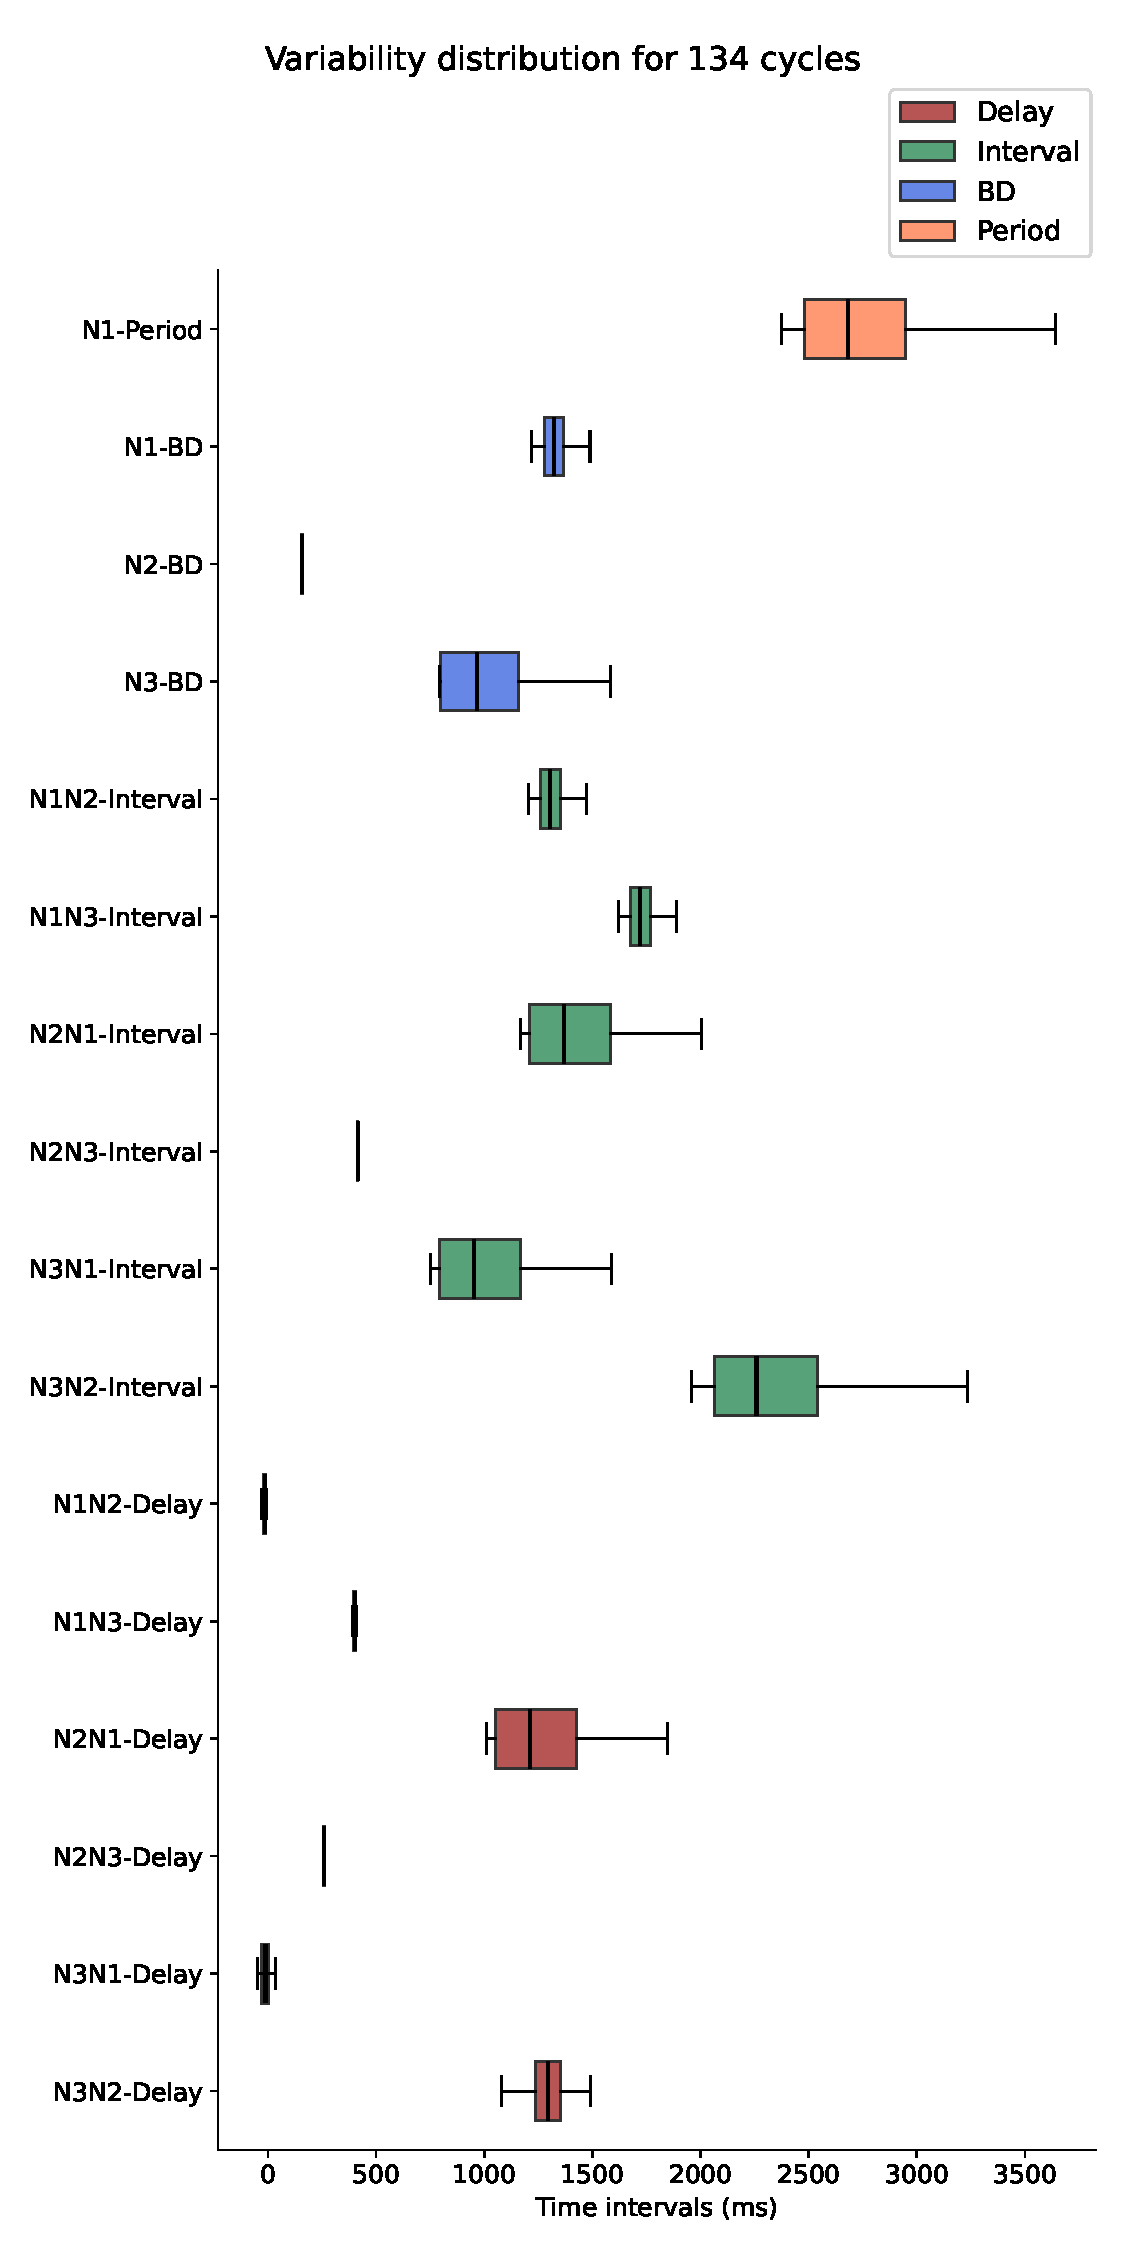
\includegraphics[width=\textwidth]{invariants/data/MODEL/n1m_driven/images/3phases/_boxplot.pdf}
	\end{minipage}
	\begin{minipage}[b]{0.53\textwidth}
		\centering
		\begin{minipage}[b]{\textwidth}
			\centering
			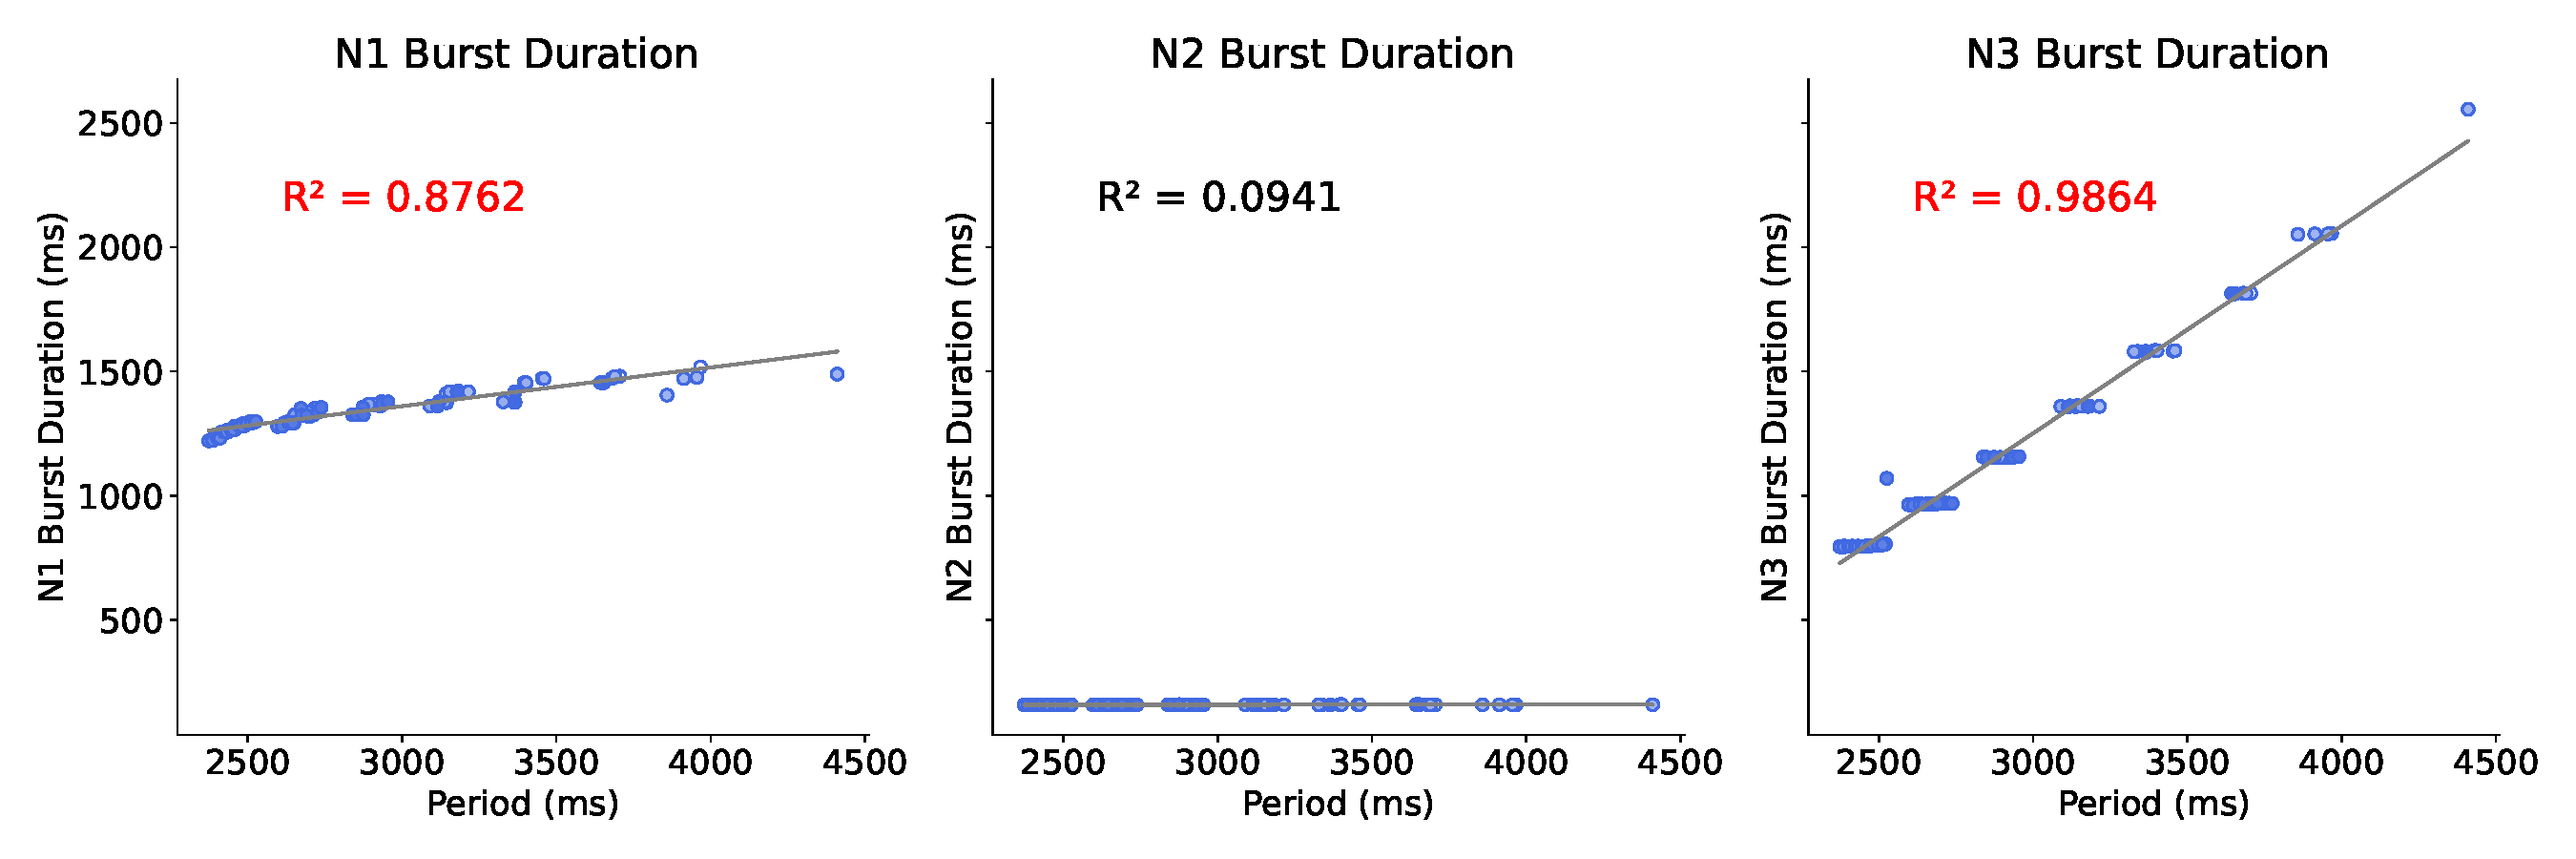
\includegraphics[width=\textwidth]{invariants/data/MODEL/n1m_driven/images/3phases/_durations.pdf}
		\end{minipage}\
		\begin{minipage}[b]{\textwidth}
			\centering
			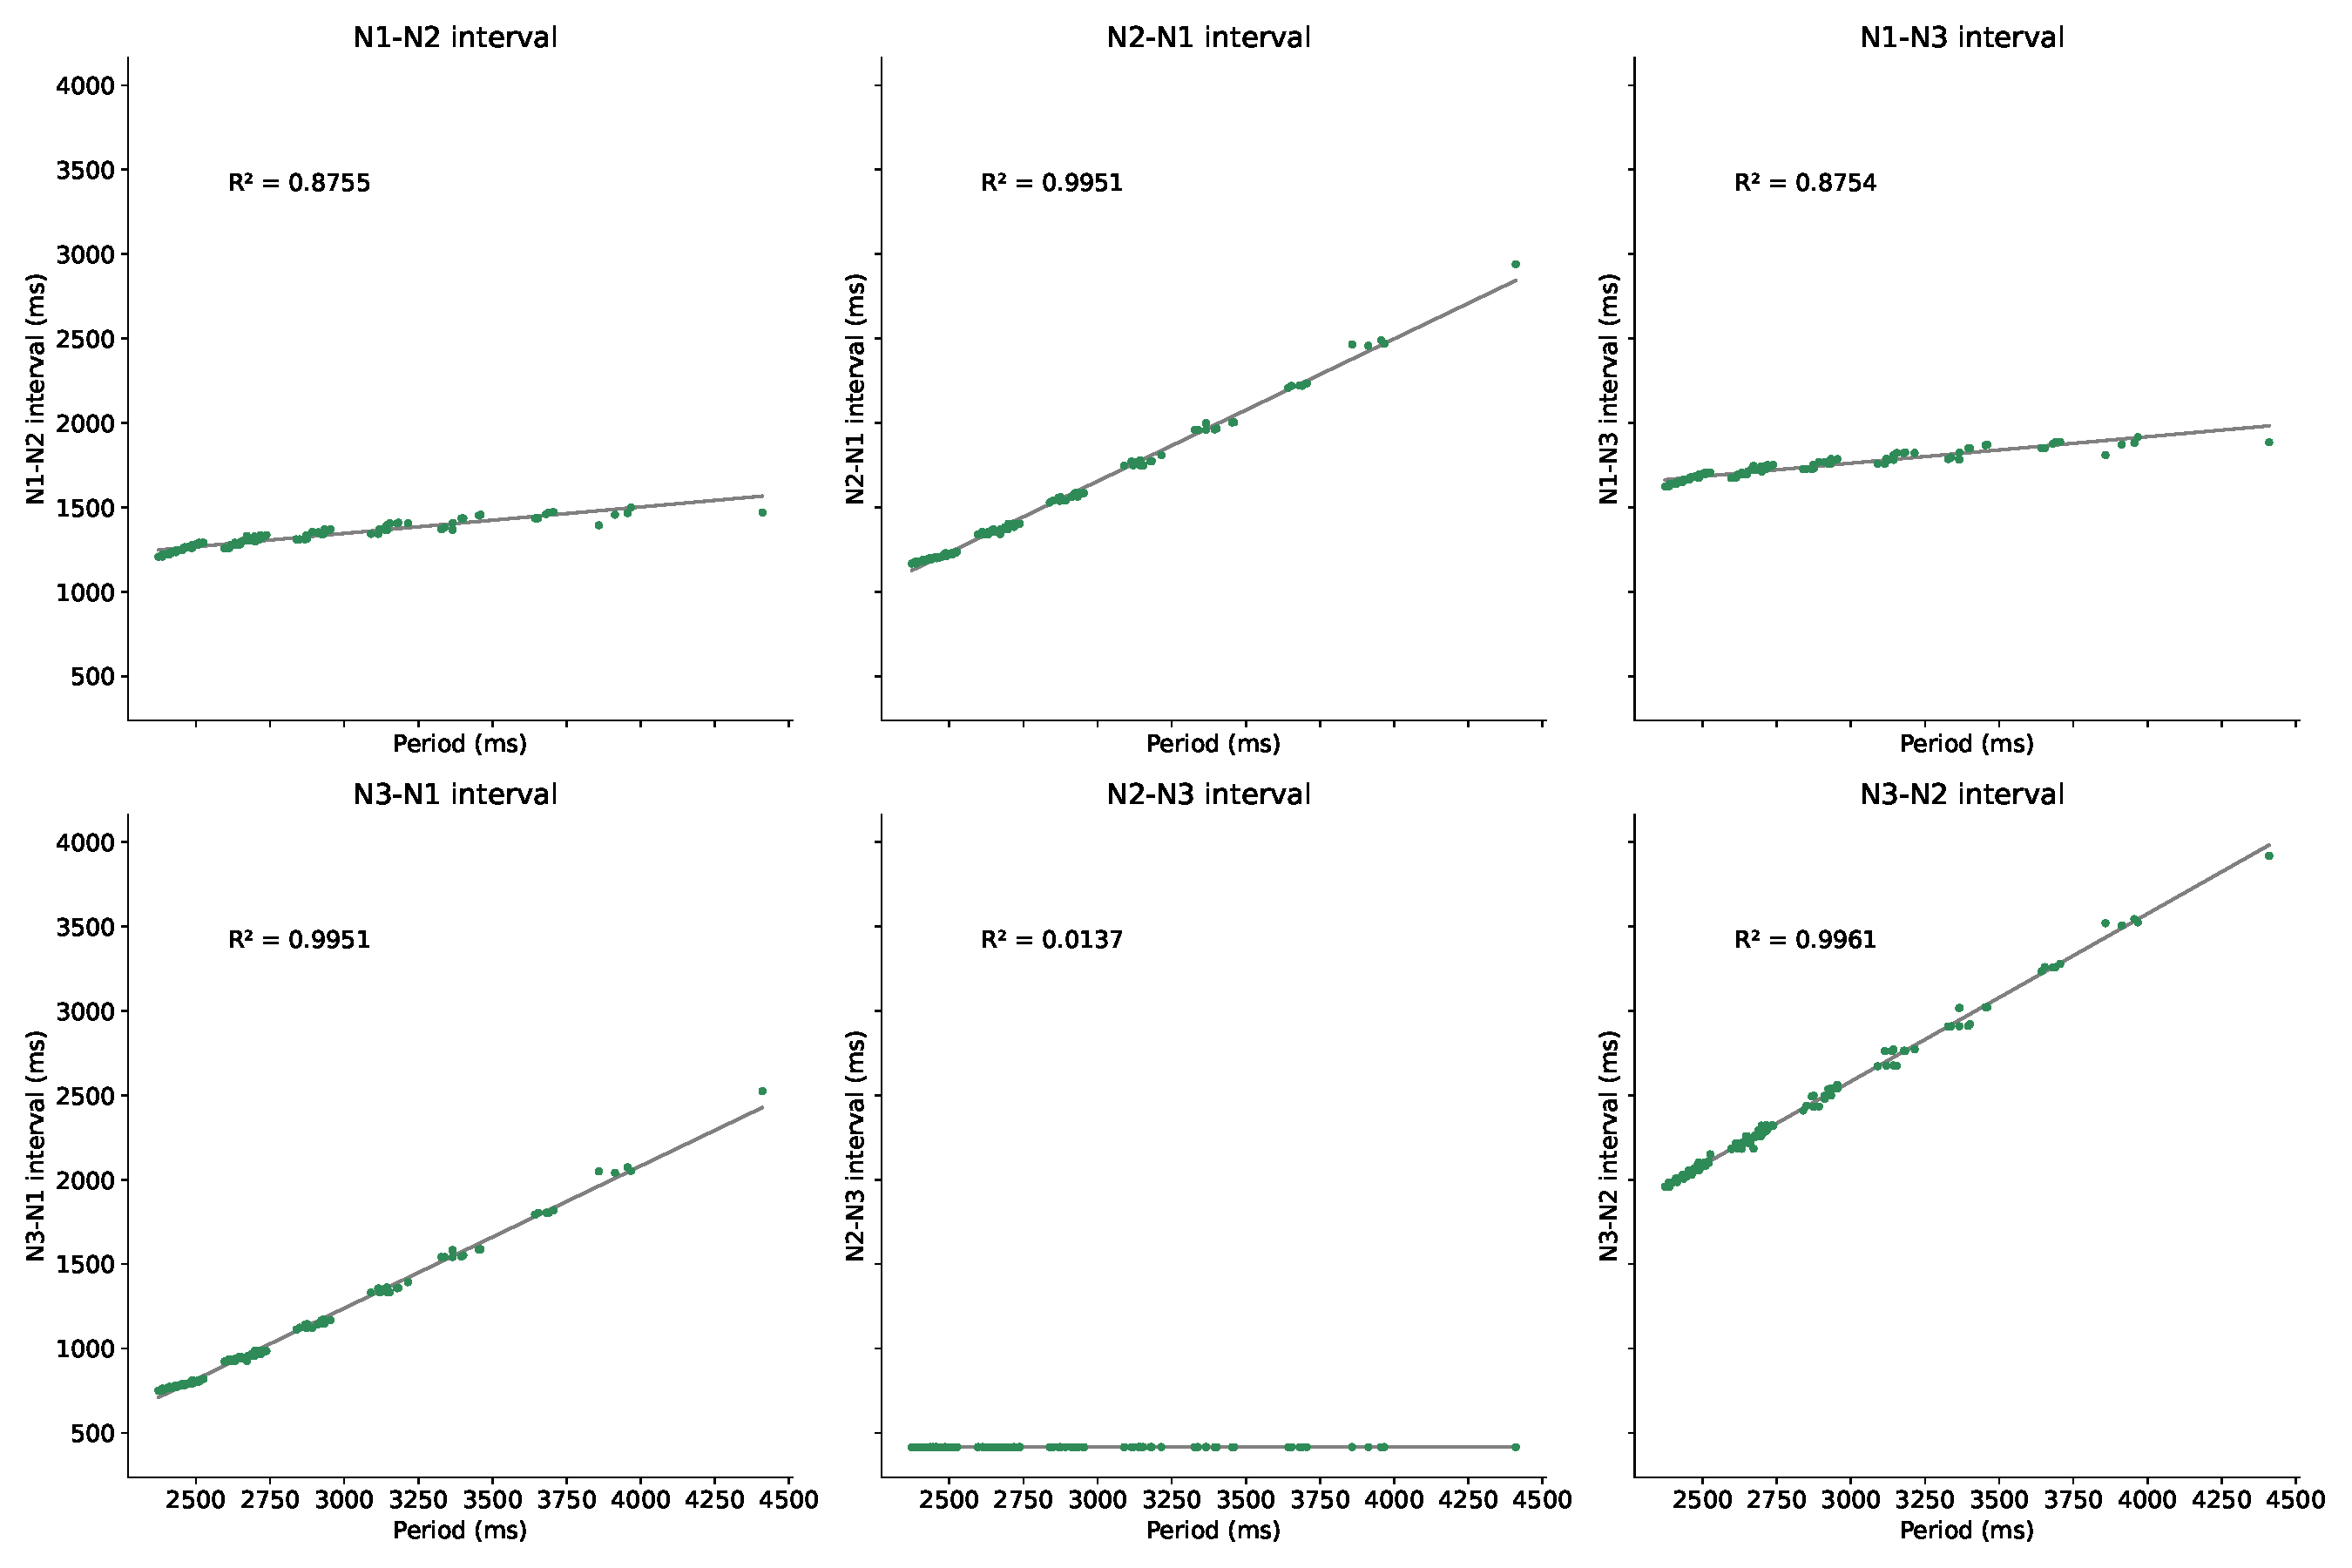
\includegraphics[width=\textwidth]{invariants/data/MODEL/n1m_driven/images/3phases/_intervals.pdf}
		\end{minipage}\
		\begin{minipage}[b]{\textwidth}
			\centering
			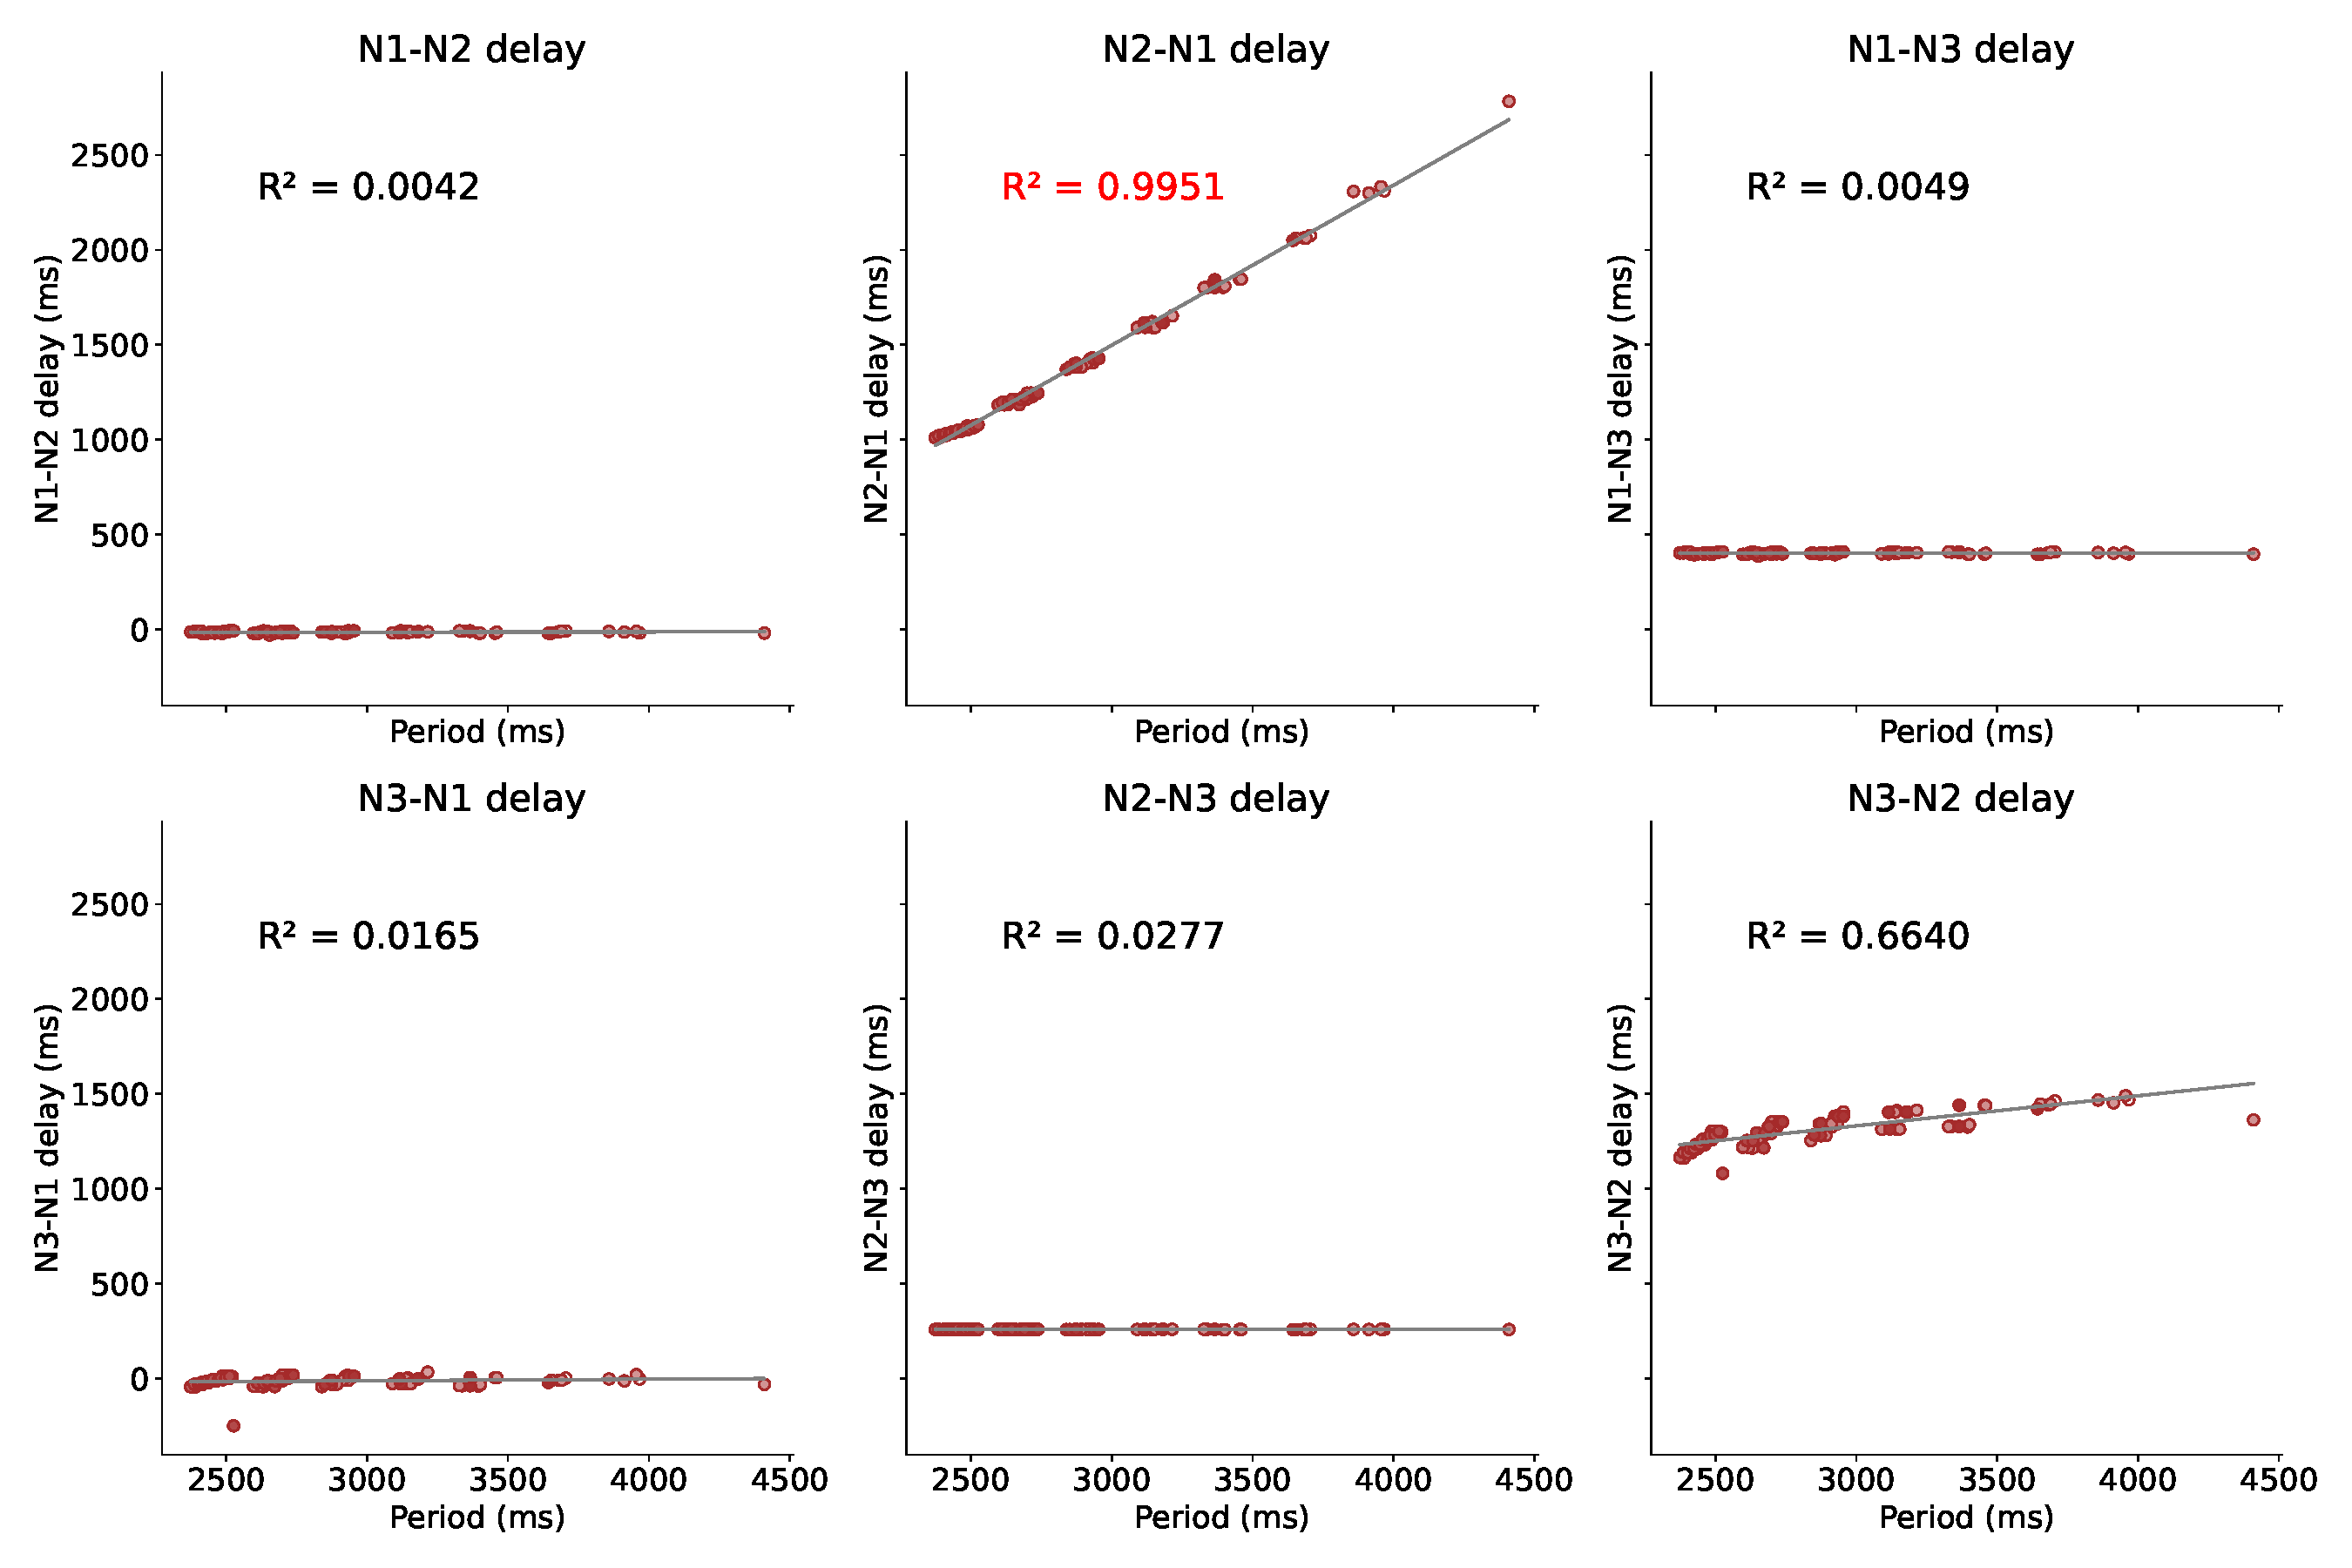
\includegraphics[width=\textwidth]{invariants/data/MODEL/n1m_driven/images/3phases/_delays.pdf}
		\end{minipage}
	\end{minipage}
	\caption{\textbf{N1M stimulation:} a) Box-plots of the  sequence intervals under N1M neuron stimulation. b) Interval correlations to period for N1M-driven simulation. First row: Burst duration. Second and third row: Two-neuron intervals. Forth and fifth row: Two-neuron delays. Linear relationships are quantified by the $R^2$ values of the linear regression.}
	\label{fig:invariant n1m}
\end{figure}

Figure \ref{fig:invariant n1m}.a) displays the boxplots of the duration of all sequence intervals defined above. Regarding burst duration of the neurons (N1M-BD, N2v-BD, N3t-BD), we can observe in this figure that the most variable one corresponds to N3t neuron. Furthermore, the derived intervals which cover N3 burst duration are also the ones presenting larger variability (i.e., N2-N1, N3-N1 and N3-N2 intervals and N2-N1 delay). On the other hand, the least variable intervals correspond to the ones related to N2v and N1M burst duration, i.e., N1-N2, N1-N3, N2-N3 intervals and N1-N2, N1-N3, N3-N1, N2-N3, N3-N2 delays. They show a nearly a constant duration during each period.

Figure \ref{fig:invariant n1m}.b) plots the cycle-by-cycle measurements of the intervals defined in \ref{fig:intervals} against the period. The first row displays burst duration intervals, which are the intervals analyzed in Elliot et al. \parencite{Elliott1991} from data obtained in electrophysiological recordings of living neurons, and in Vavoulis et al. from data obtained in model simulations \parencite{vavoulis_computational_2007}. The results shown in this row match those results, being N3t-BD the most correlated to the period, which can be noted by the $R^2$ value close to one in the linear regression. The other two intervals (N1M-BD and N2v-BD), which were also the least variable, are not strongly correlated to the period. 

Likewise, the most variable intervals derived from other time references of the sequence also show a high correlation with the period, i.e., they present dynamical invariants, in this case N2-N1, N3-N1, N3-N2 intervals and N2-N1 delay. The cycle-by-cycle period variability is a consequence of the variability in these specific intervals.

On the other hand, intervals related to neuron N2v and N1M are the least variable. N2v is the one least affected by the global activity of the circuit, in terms of its burst duration. Moreover, some of the intervals are very short, or even negative, since the end of a given neuron's burst overlaps the next one's beginning (N1-N2 and N3-N1 delay). This is the case for N1-N2 and N3-N1 delay (4th row, 1st column and 5th row, 1st column, respectively in Fig. \ref{fig:invariant n1m}.b).  




\subsection{N3t driven variability}
\label{subsec:n3t driven}

The stimulation protocol was also applied to N3t neuron. In spite that no previous analysis on injecting a current ramp into this neuron has been reported neither experimentally nor in the feeding CPG computational model, due to the connectivity in the circuit, it can be expected that stimulation of N3t will induce variability in the rhythm. The characterization of the sequence intervals in this case are shown in Fig. 
\ref{fig:invariants n3t}.a) and the correlation analysis is displayed in Fig. \ref{fig:invariants n3t}.b).
%In fact, we can expect a similar result to N1M-driven simulation because of their bidirectional connectivity see Fig. \ref{fig:CPG diagram}.  ***dicutir si es siméterica o no *****


Results shown in Fig. \ref{fig:invariants n3t}.a) indicate that the larger variability is present in the same intervals related to N3t burst duration, as when the stimulation was delivered to N1M. However, in this simulation we observe that N1M had a lower variability while N3t had a higher variability with respect to the previous condition. 
%: N1M decreased its variability while N3t has increased it *****discutir***. 
In contrast, N2v-BD maintained its variability, as well as all the derived intervals containing this burst duration.

Note that N3-N1 delay, which is the interval from the end of the N3t burst to the beginning of N1M burst, shows negative values. This means that neuron N1M started earlier than the end of N3t in every cycle. Whilst this was also present in N1M-driven activity, here the variability of this interval is much higher, leading to a larger overlapping.
% N2v maintains its variability, being this interval and all the intervals related to it the least variable. Hence, in the distribution of the activity in the circuits between the neurons, the main negotiation is between N1M and N3t, distributing the variability and the period leading between they both. ***esto también lo tenemos que pulir un poco****

Figure \ref{fig:invariants n3t}.b) plots each interval duration against the period. As in the previous condition, the dynamical invariants (i.e. intervals presenting a strong correlation to the period) show up in the intervals related to N3t, which were the ones presenting also the highest variability, whereas those intervals that do not participate in dynamical invariants, are the ones related to N1M and mostly N2v (the least variable ones). 


%The linear relationships regarding the least variable intervals (related to N2v and N1M burst durations), also present similar results to those discussed above when the rhythm was driven by N1M. Hence, the intervals most correlated are the ones with higher variability, whereas those intervals that do not participate in dynamical invariants, are the ones related to N1M and mostly N2v (the least variable ones).
%***revisar redundancia***


\begin{figure}[hbt!]
	\begin{minipage}[b]{0.45\textwidth}
		\centering
		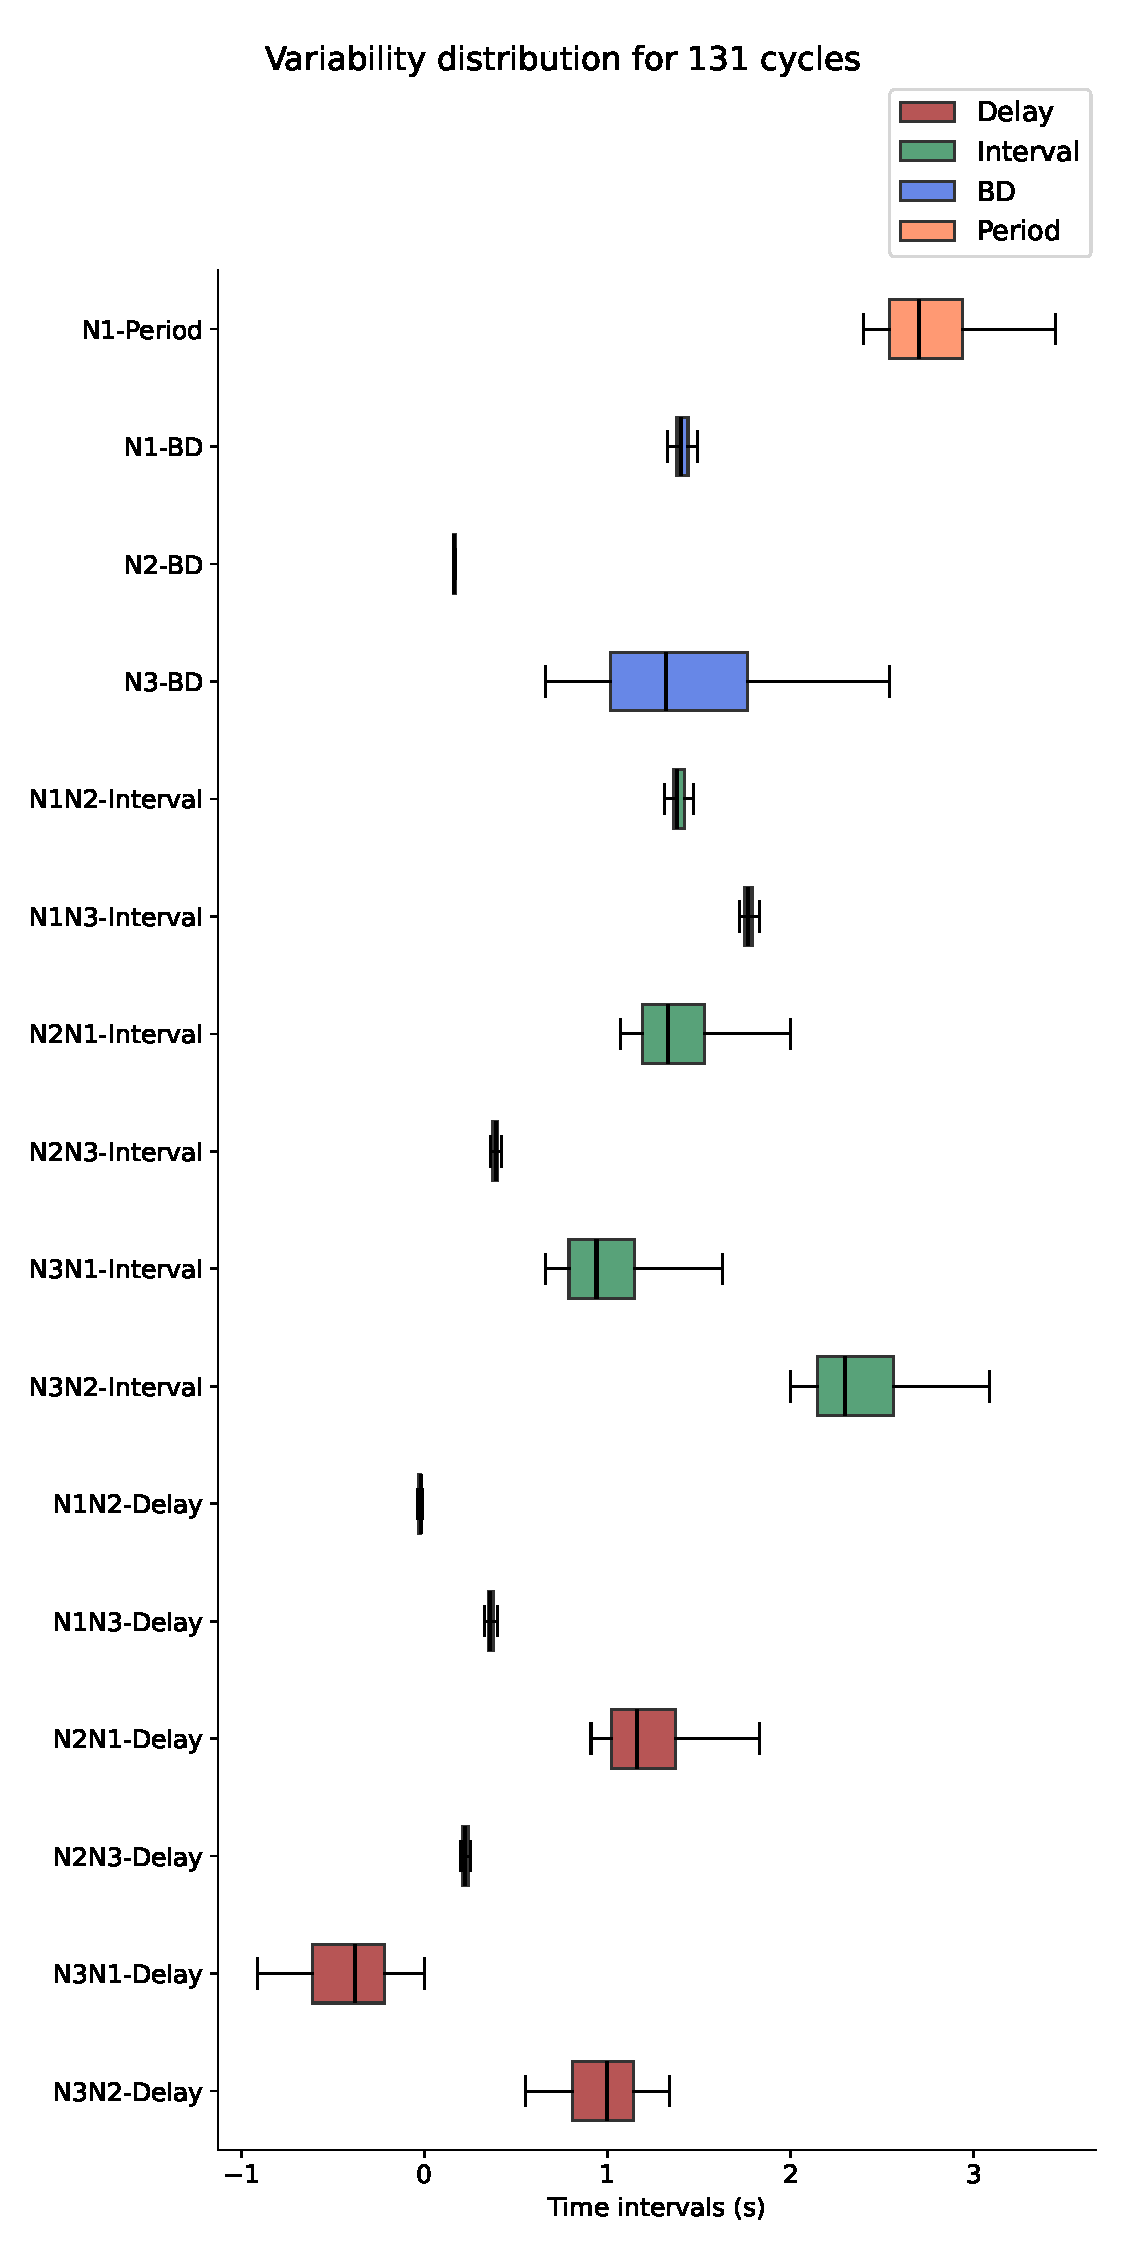
\includegraphics[width=\textwidth]{invariants/data/MODEL/n3t_driven/images/3phases/_boxplot.pdf}
	\end{minipage}
	\begin{minipage}[b]{0.53\textwidth}
		\centering
		\begin{minipage}[b]{\textwidth}
			\centering
			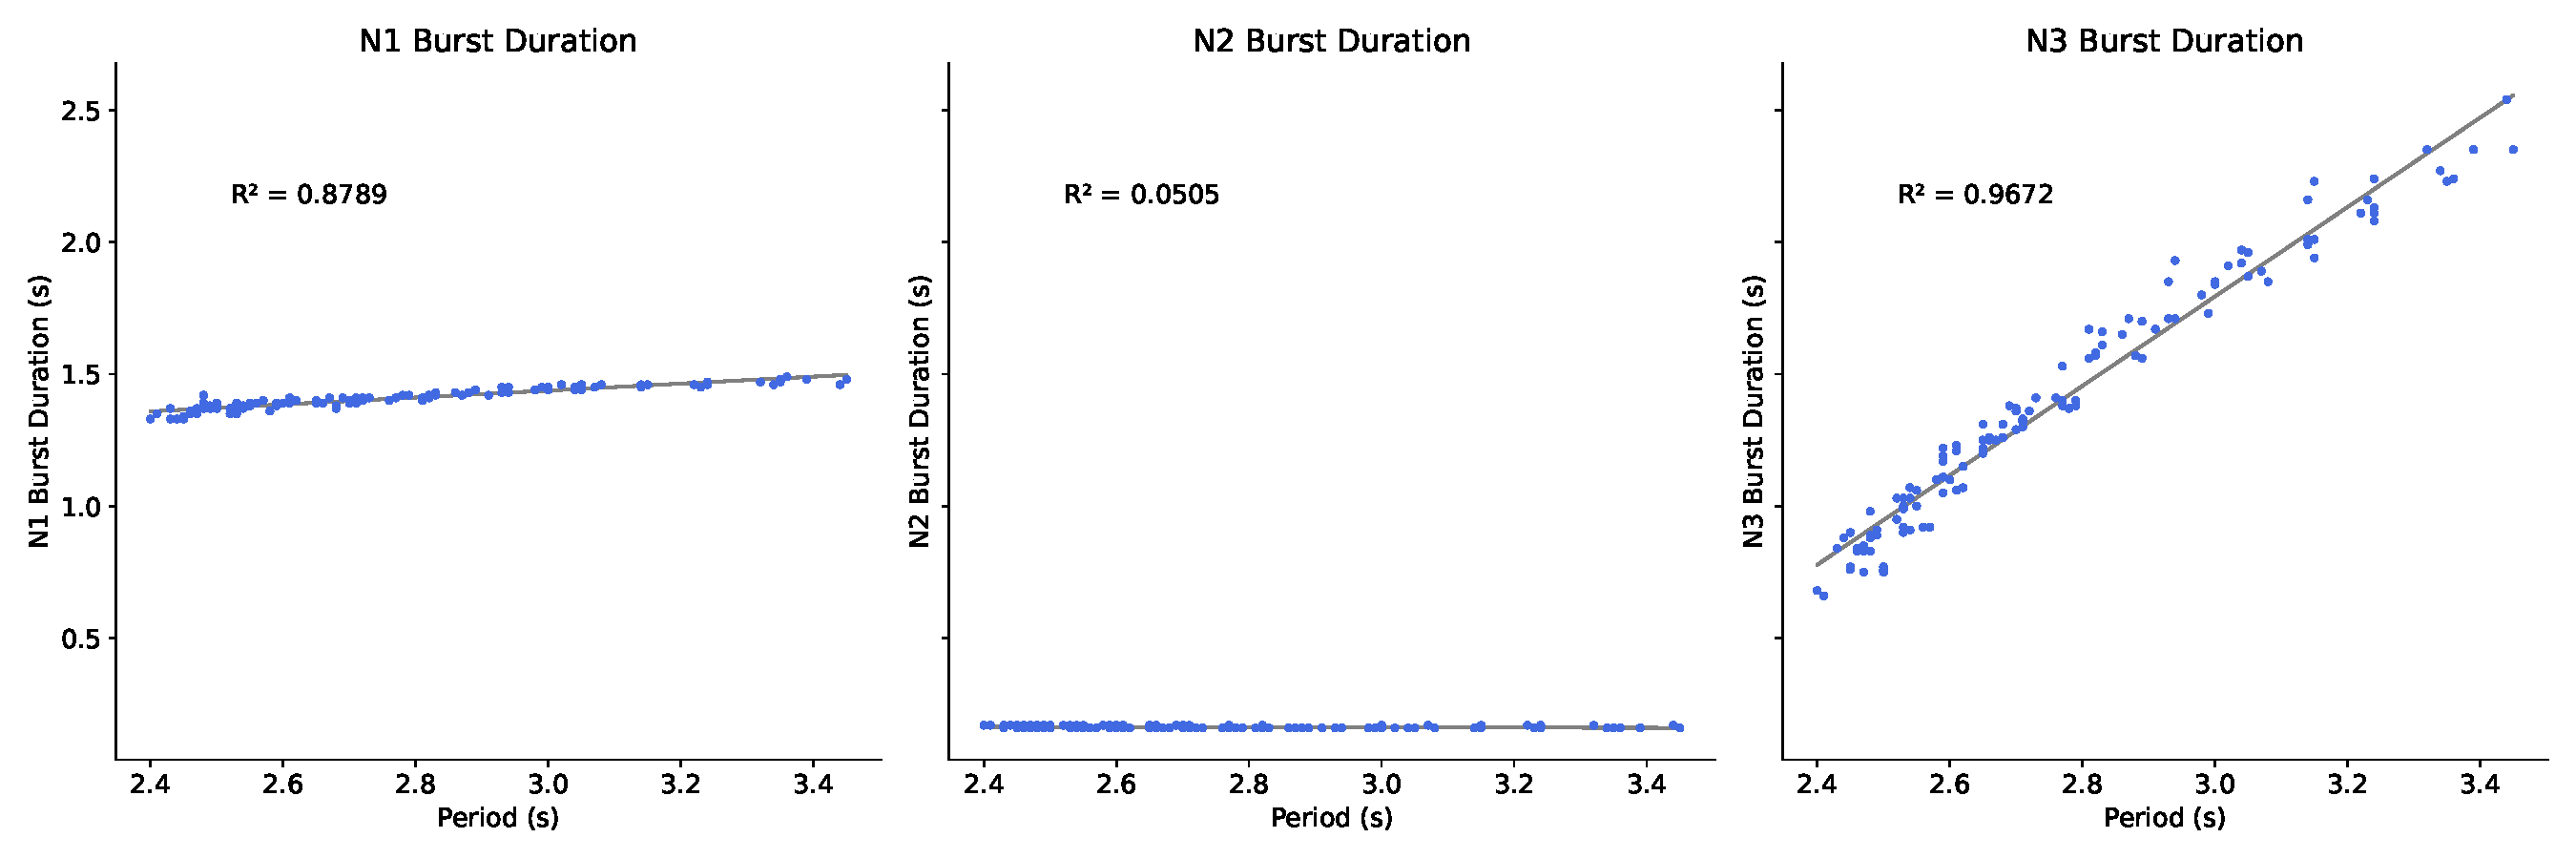
\includegraphics[width=\textwidth]{invariants/data/MODEL/n3t_driven/images/3phases/_durations.pdf}
		\end{minipage}\
		\begin{minipage}[b]{\textwidth}
			\centering
			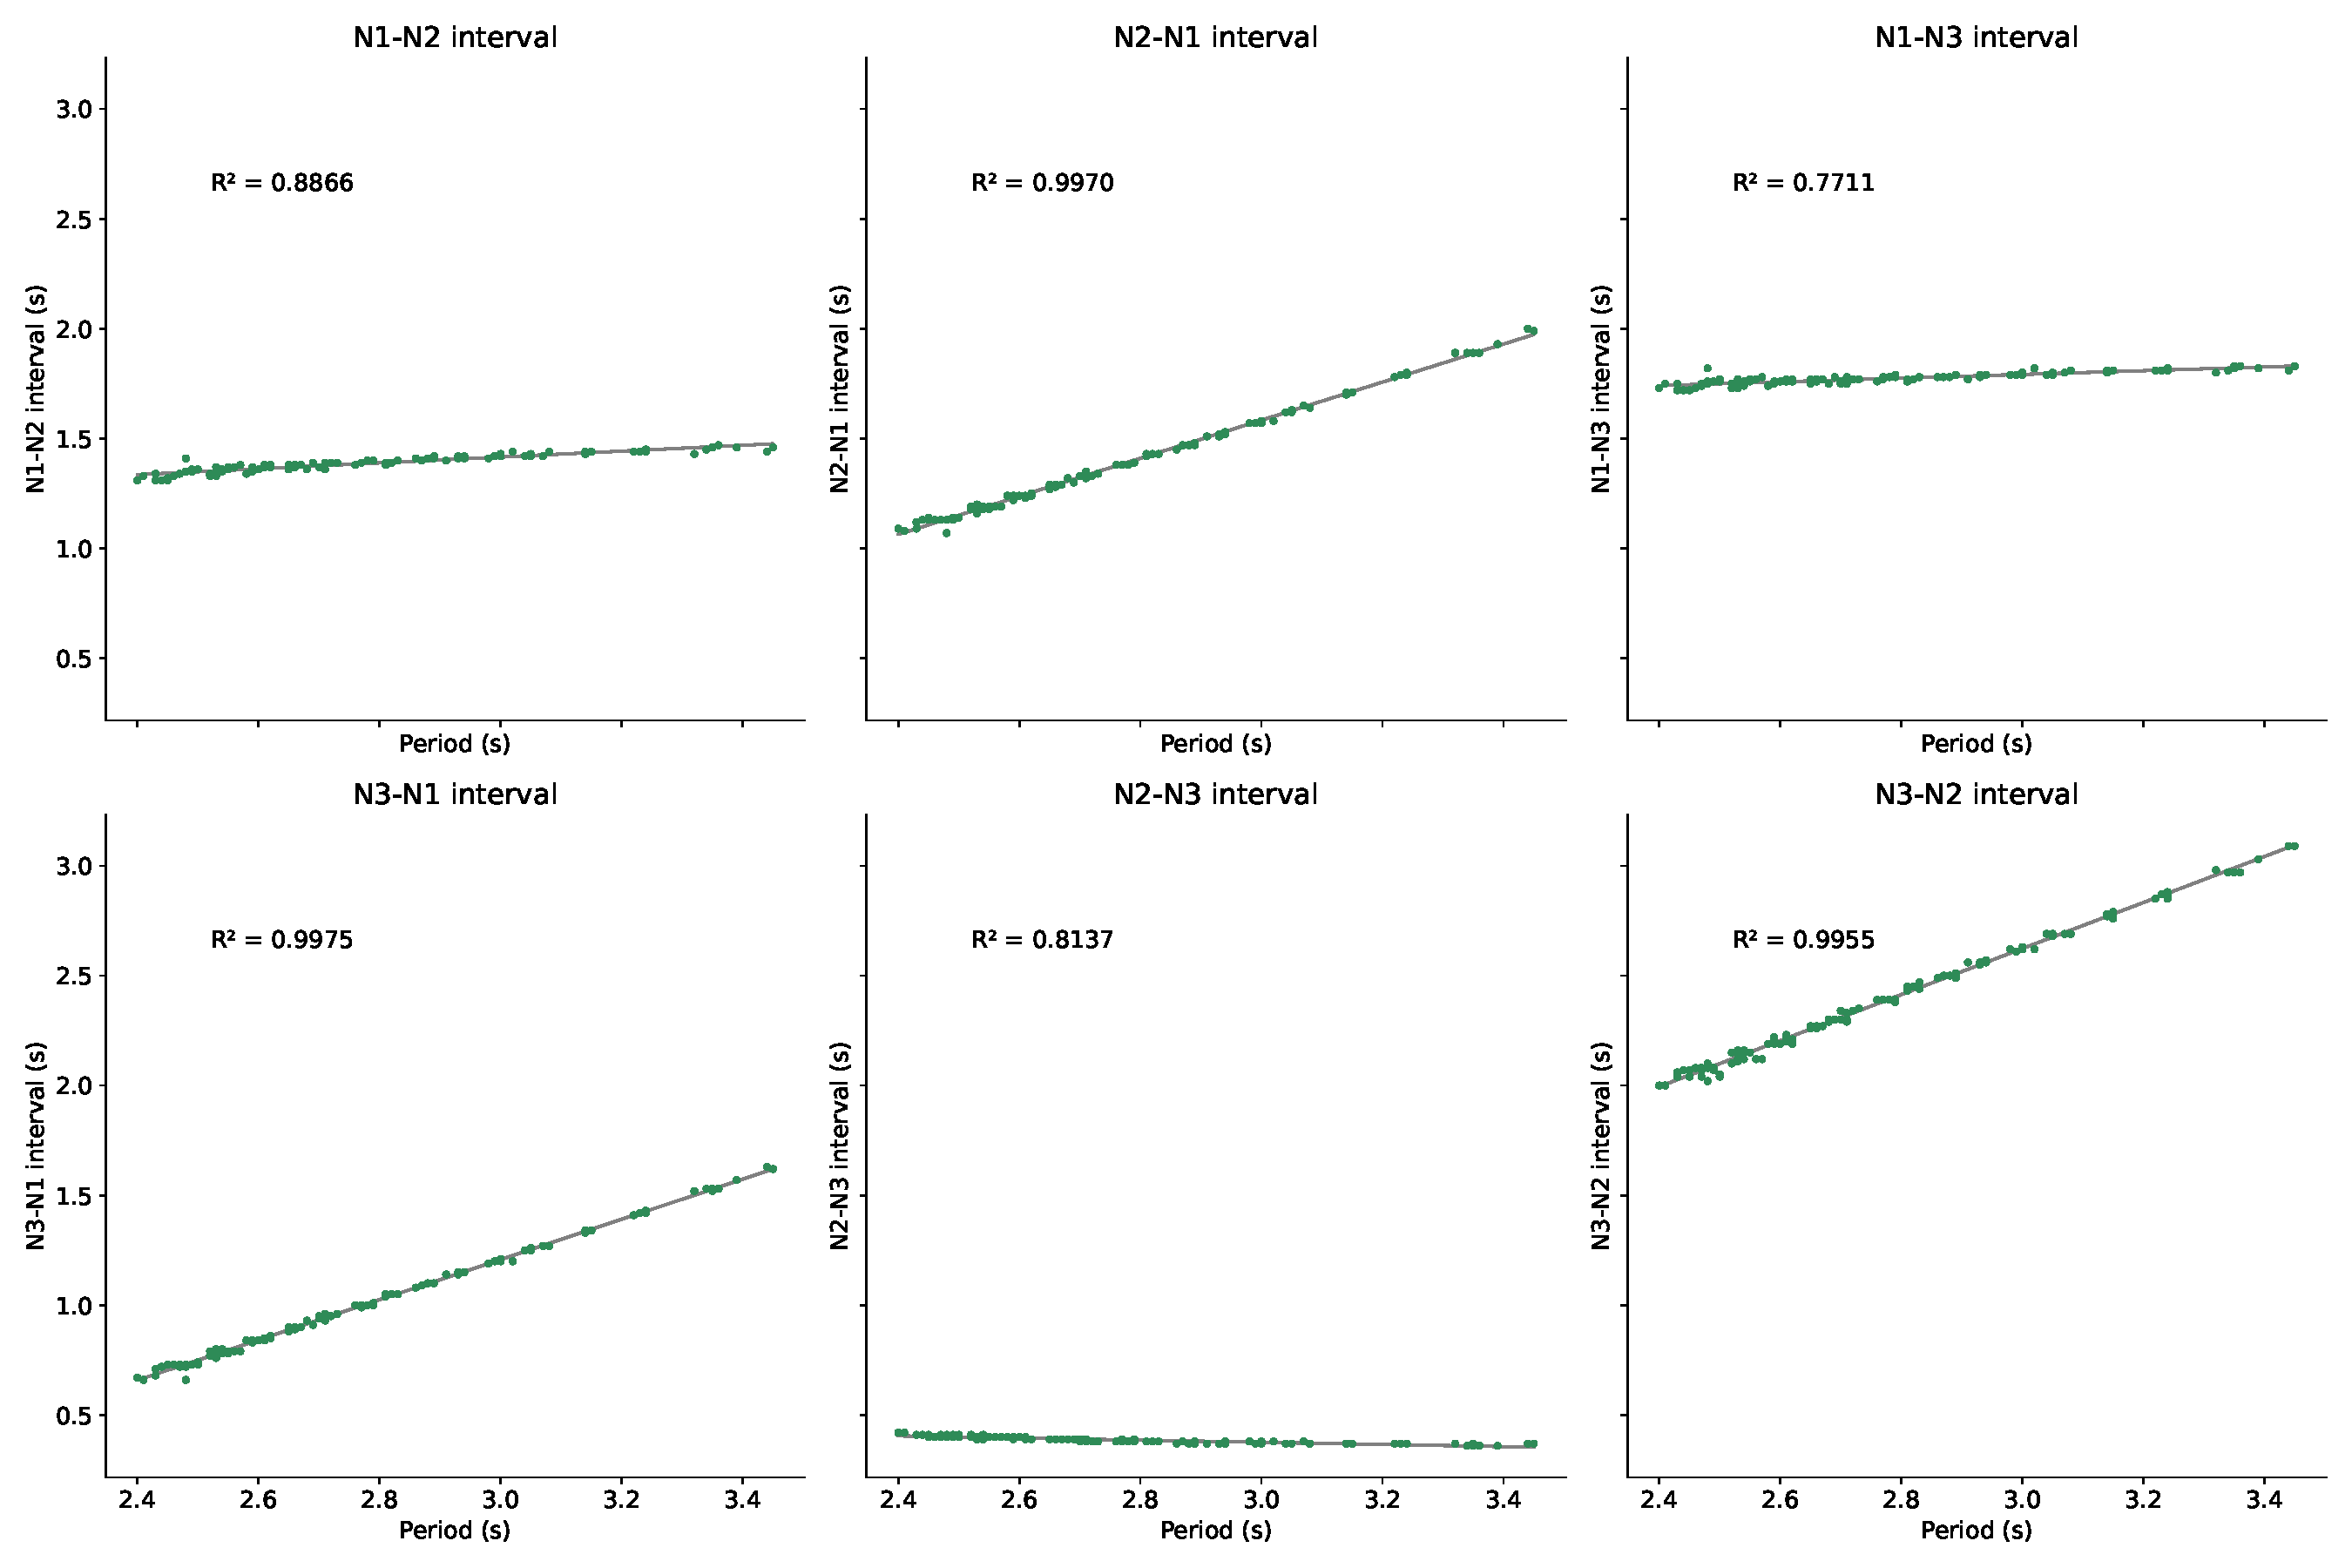
\includegraphics[width=\textwidth]{invariants/data/MODEL/n3t_driven/images/3phases/_intervals.pdf}
		\end{minipage}\
		\begin{minipage}[b]{\textwidth}
			\centering
			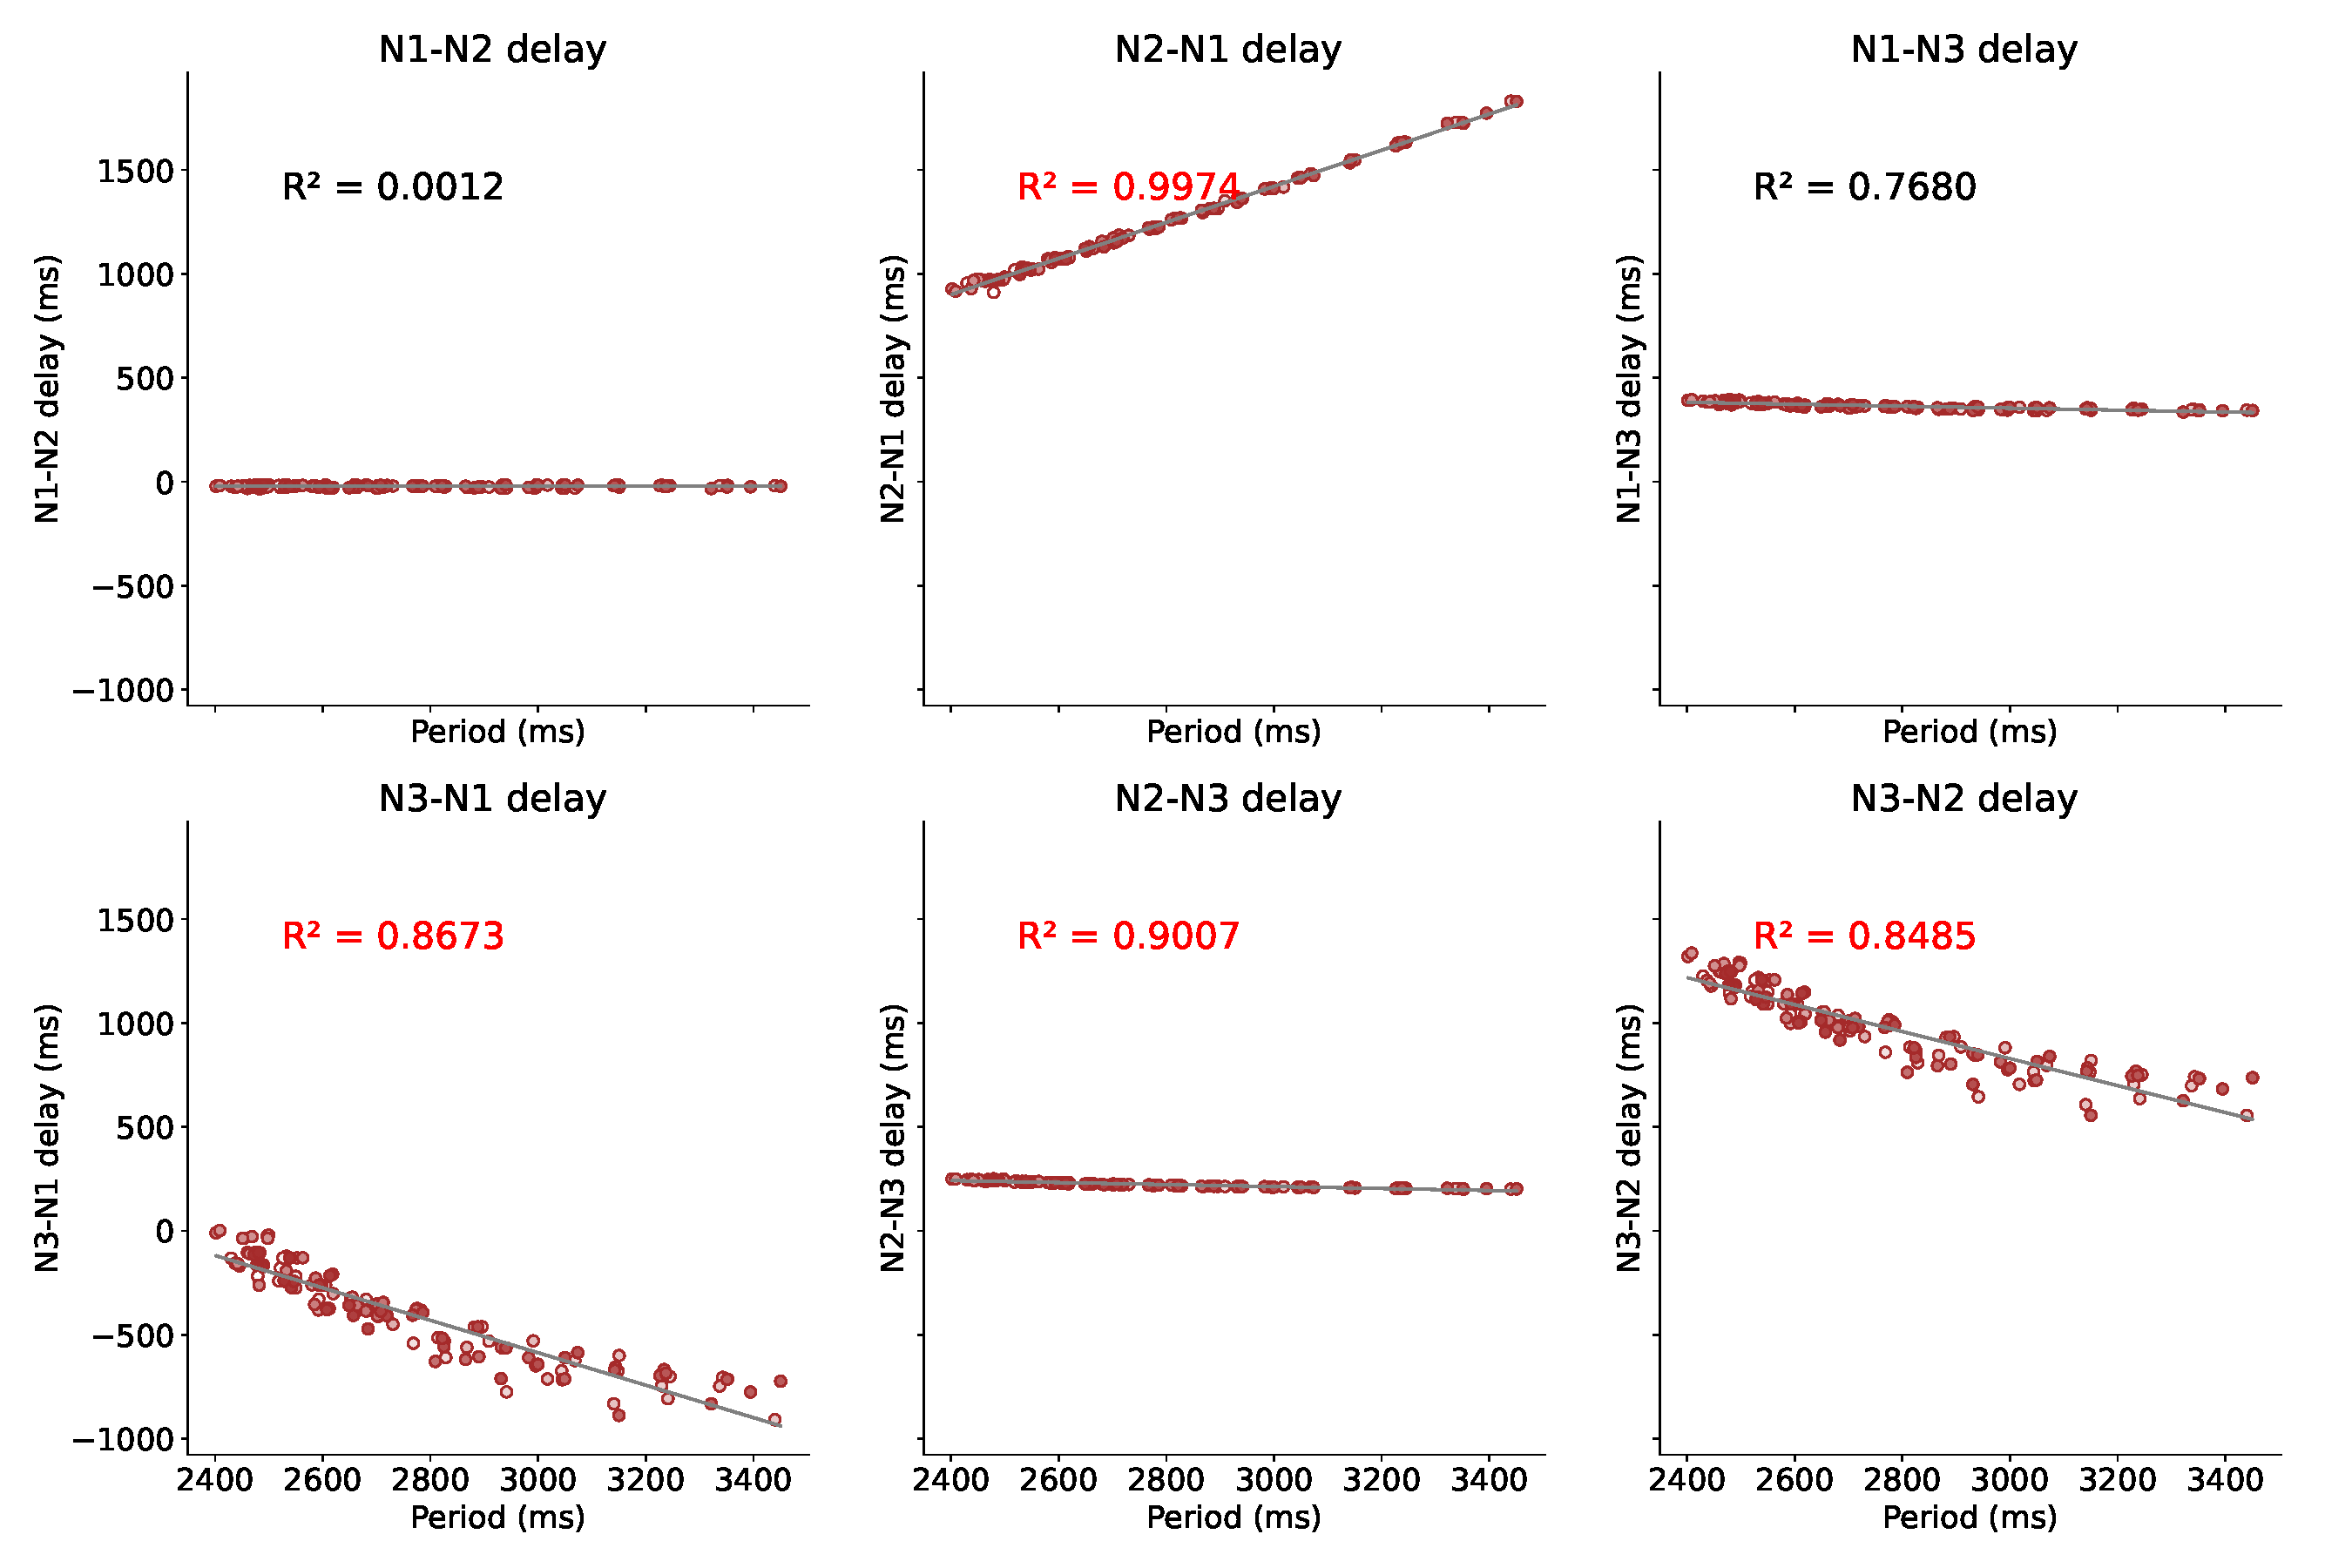
\includegraphics[width=\textwidth]{invariants/data/MODEL/n3t_driven/images/3phases/_delays.pdf}
		\end{minipage}
	\end{minipage}
	\caption{\textbf{N3t stimulation:} a) Box-plots of the sequence intervals under N3t neuron stimulation. b) Interval correlations to Period for N3t-driven simulation. First row: Burst duration. Second and third row: Two-neuron intervals. Forth and fifth row: Two-neuron delays.}
	\label{fig:invariants n3t}
\end{figure}





\subsection{SO driven variability}
\label{subsec:so driven}

The same protocol was implemented with a ramp stimulation applied to SO to induce variability, using the injected current values shown in Table \ref{table:inj values} for each neuron. Events were detected and all intervals were measured (Fig. \ref{fig:intervals}) and their variability was characterized. %This neuron has also been used in previous studies with stimulation protocols both in electrophysiological experiments and in model simulations due to its important role in rhythm activation and modulation. ***se podría quitar, si no hay que poner las referencias otra vez****

\begin{figure}[hbt!]
	\begin{minipage}[b]{0.45\textwidth}
		\centering
		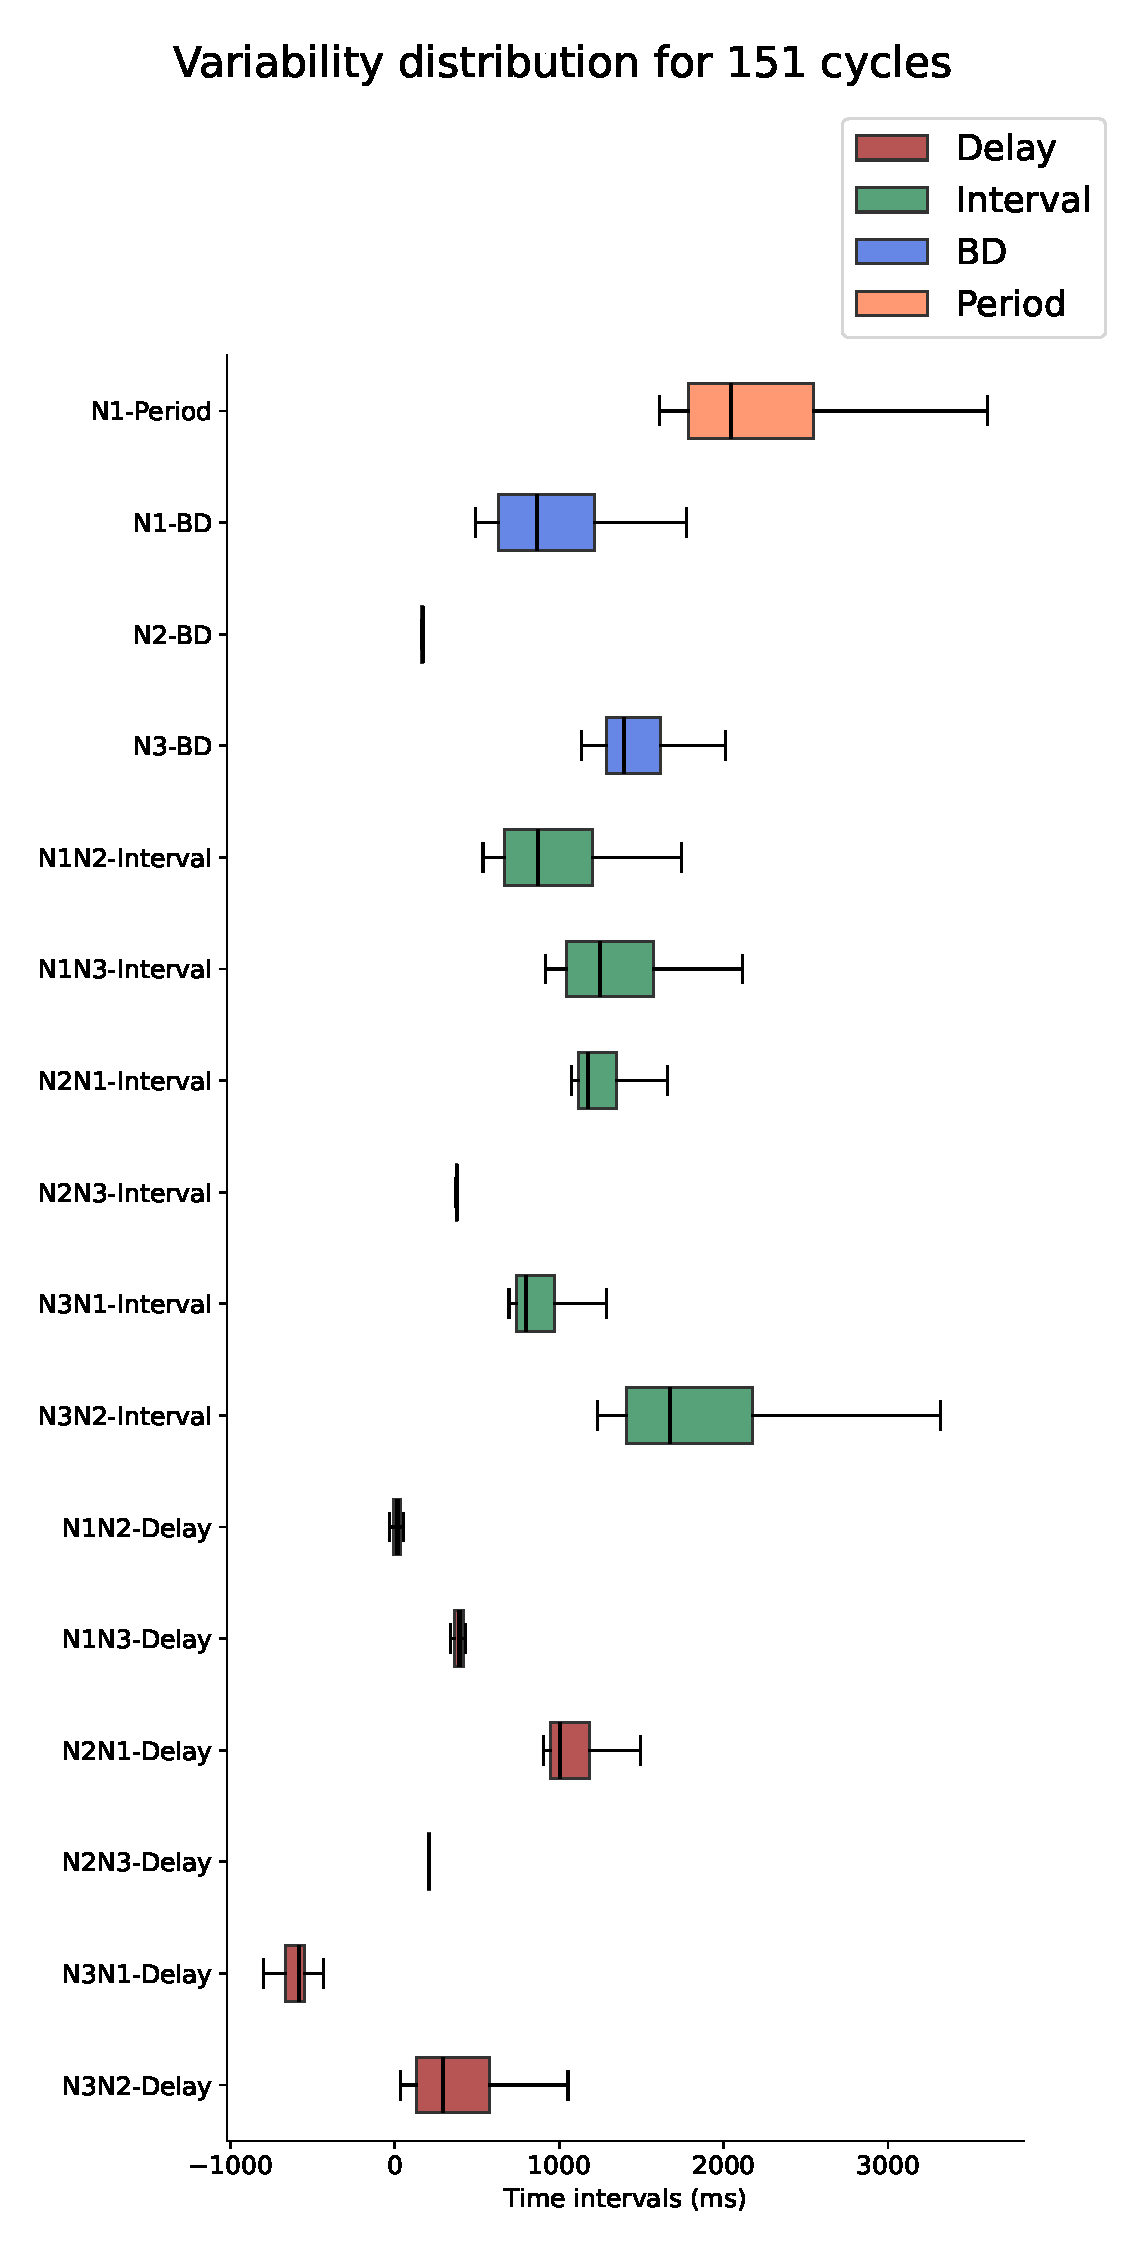
\includegraphics[width=\textwidth]{invariants/data/MODEL/so_driven/images/3phases/_boxplot.pdf}
	\end{minipage}
	\begin{minipage}[b]{0.53\textwidth}
		\centering
		\begin{minipage}[b]{\textwidth}
			\centering
			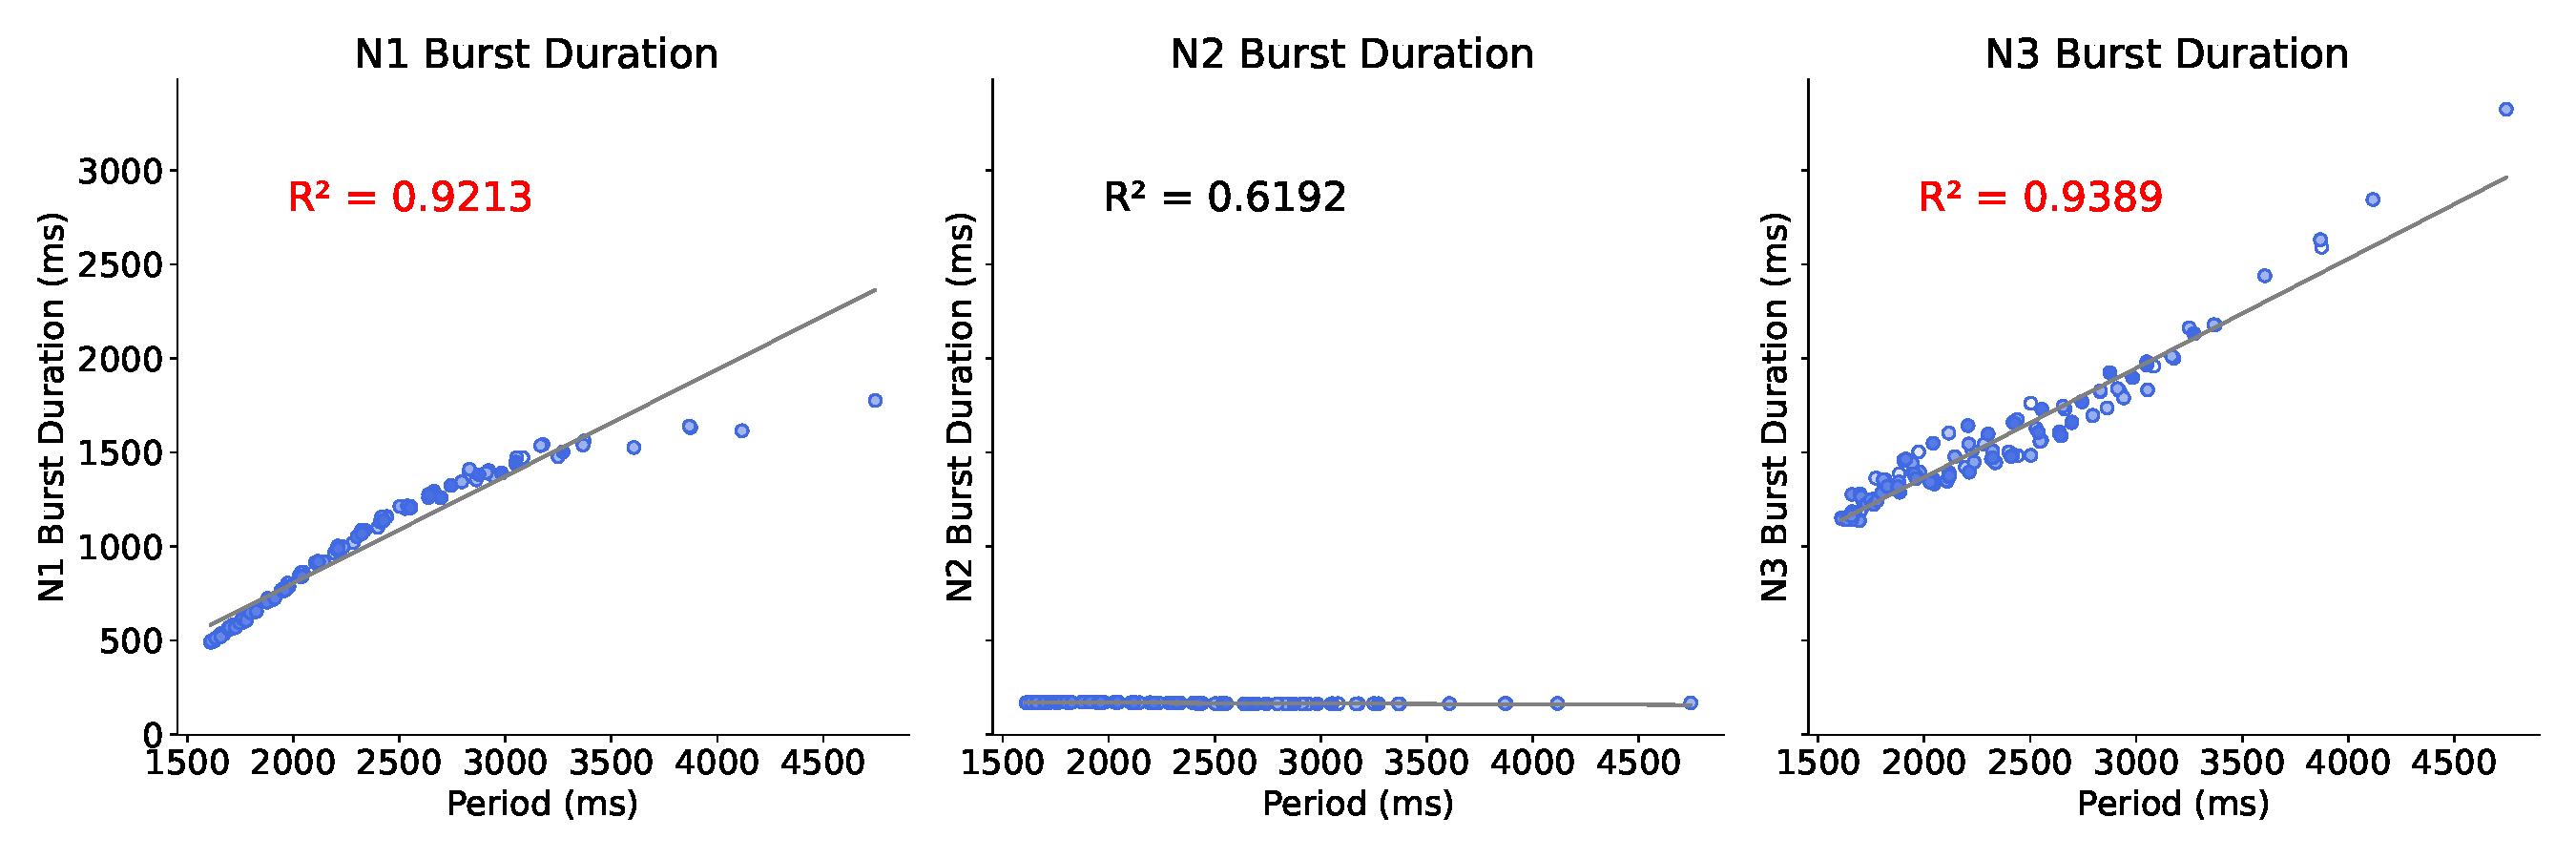
\includegraphics[width=\textwidth]{invariants/data/MODEL/so_driven/images/3phases/_durations.pdf}
		\end{minipage}\
		\begin{minipage}[b]{\textwidth}
			\centering
			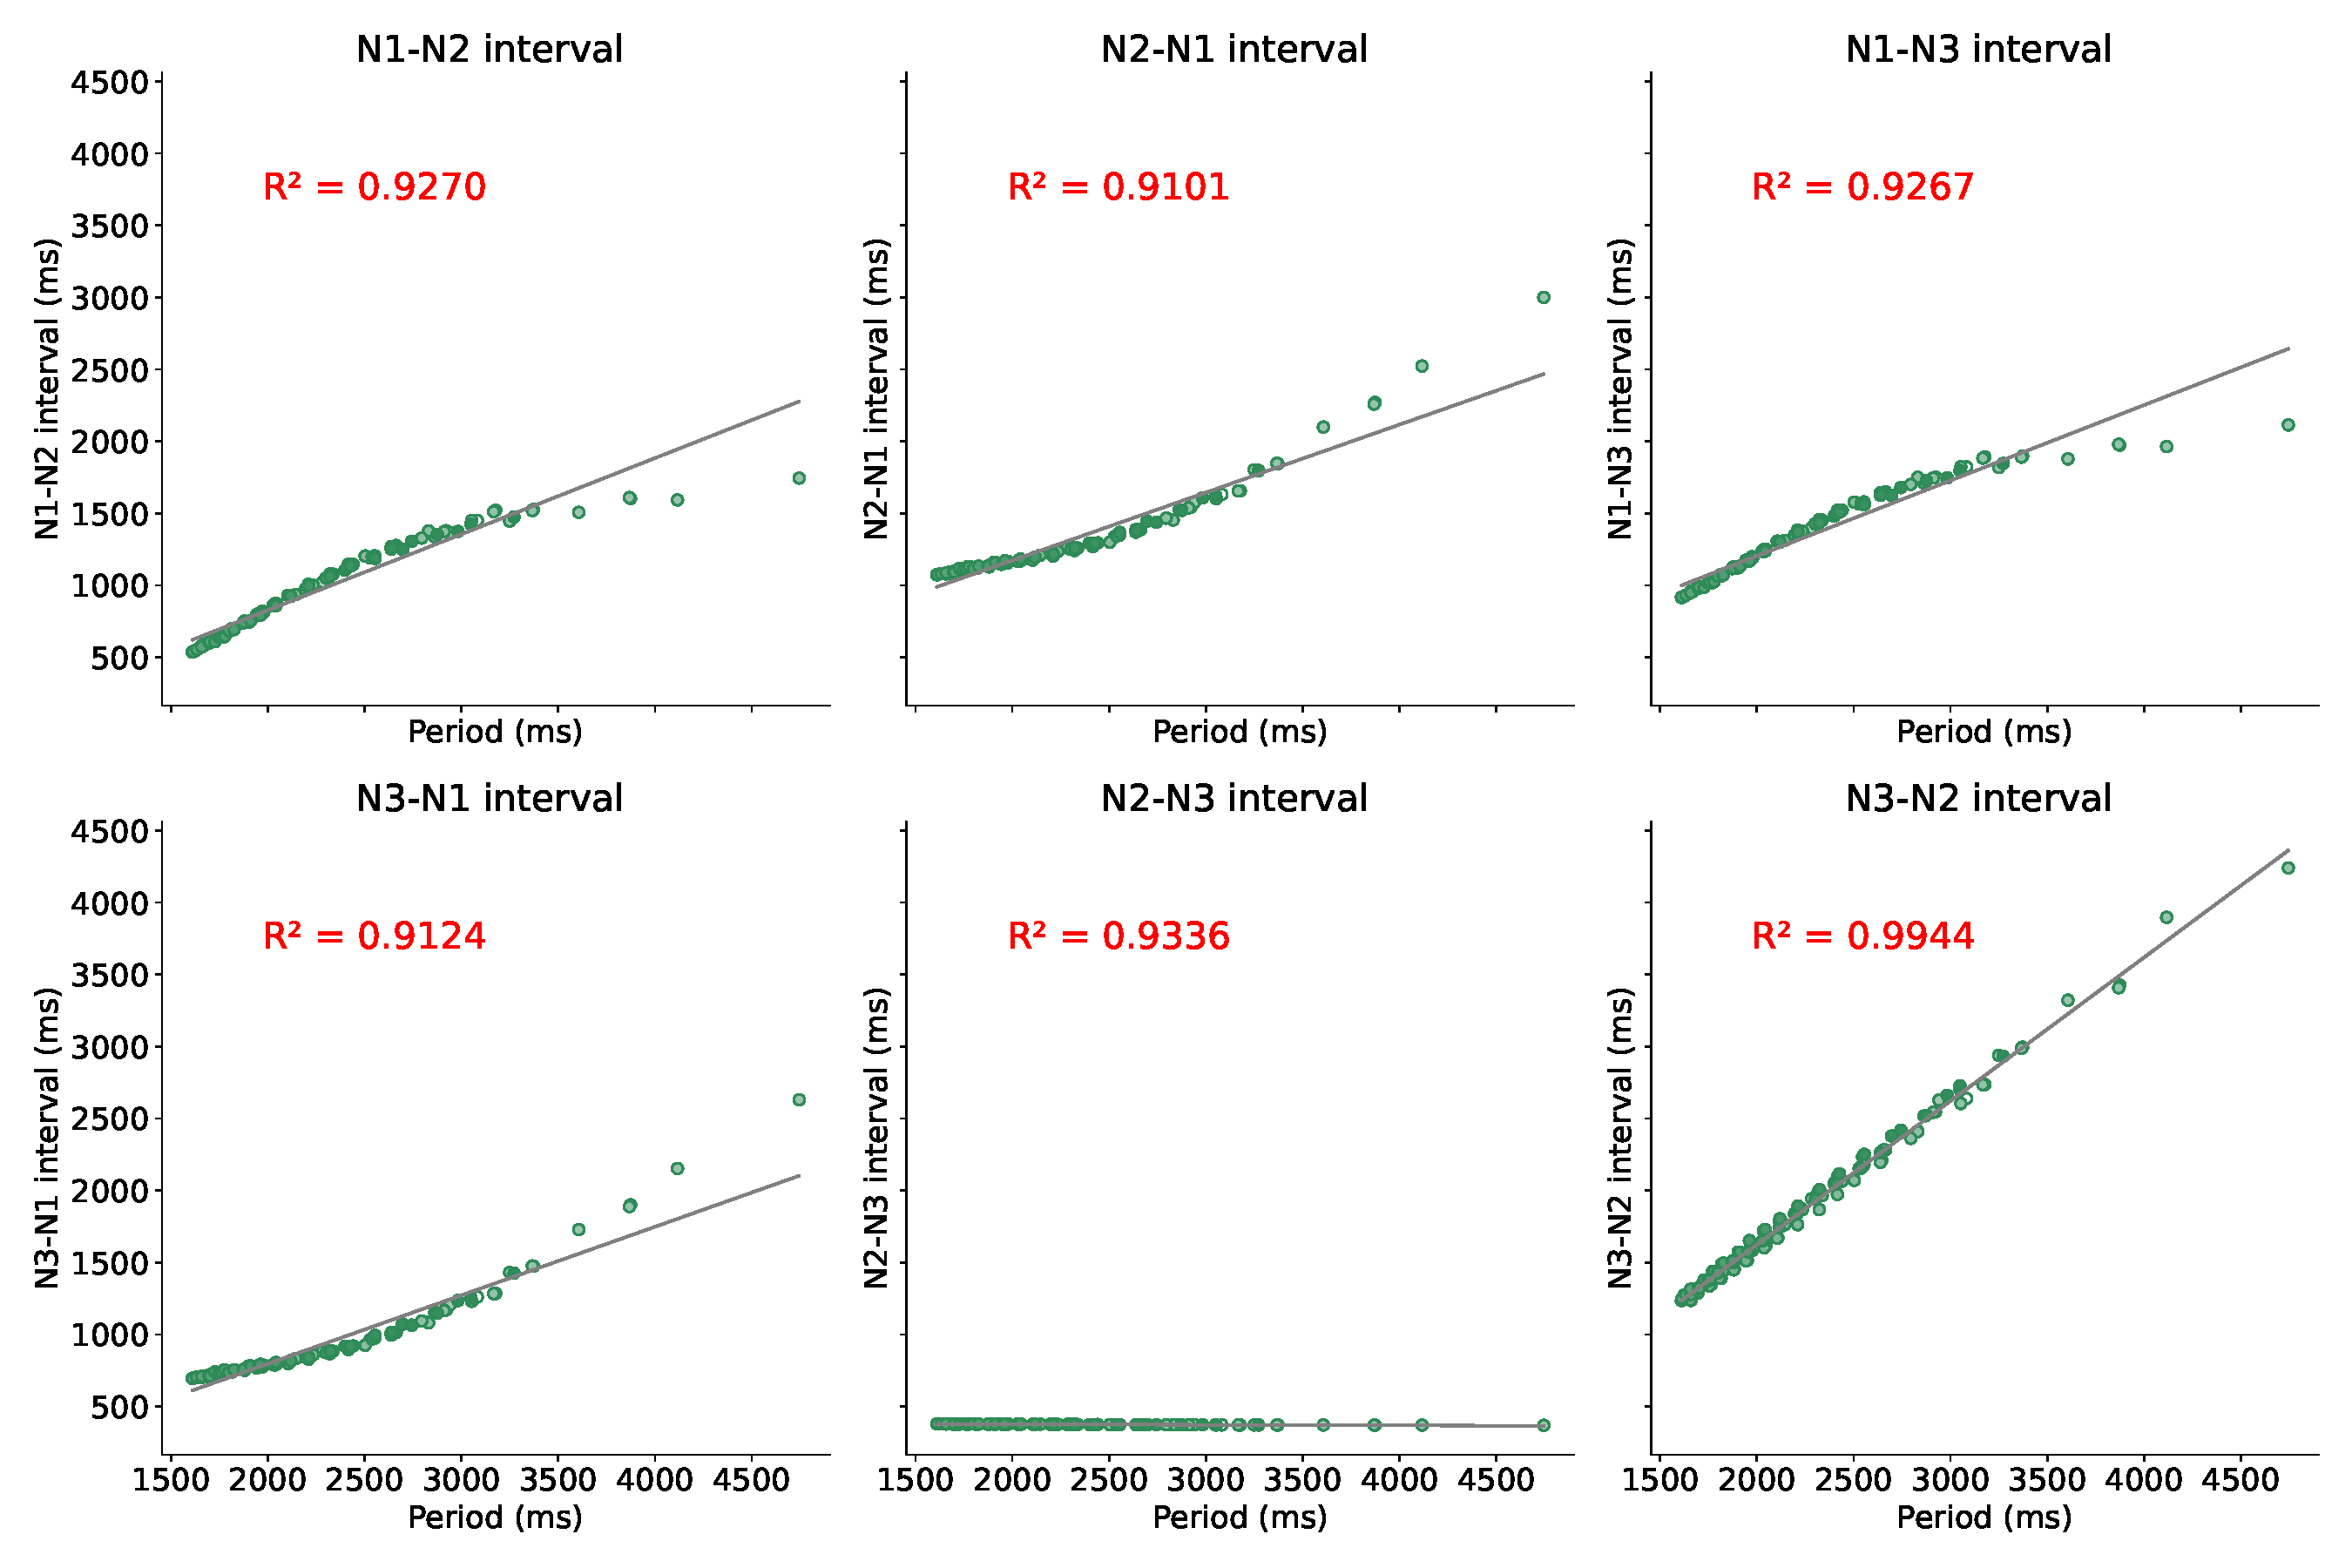
\includegraphics[width=\textwidth]{invariants/data/MODEL/so_driven/images/3phases/_intervals.pdf}
		\end{minipage}\
		\begin{minipage}[b]{\textwidth}
			\centering
			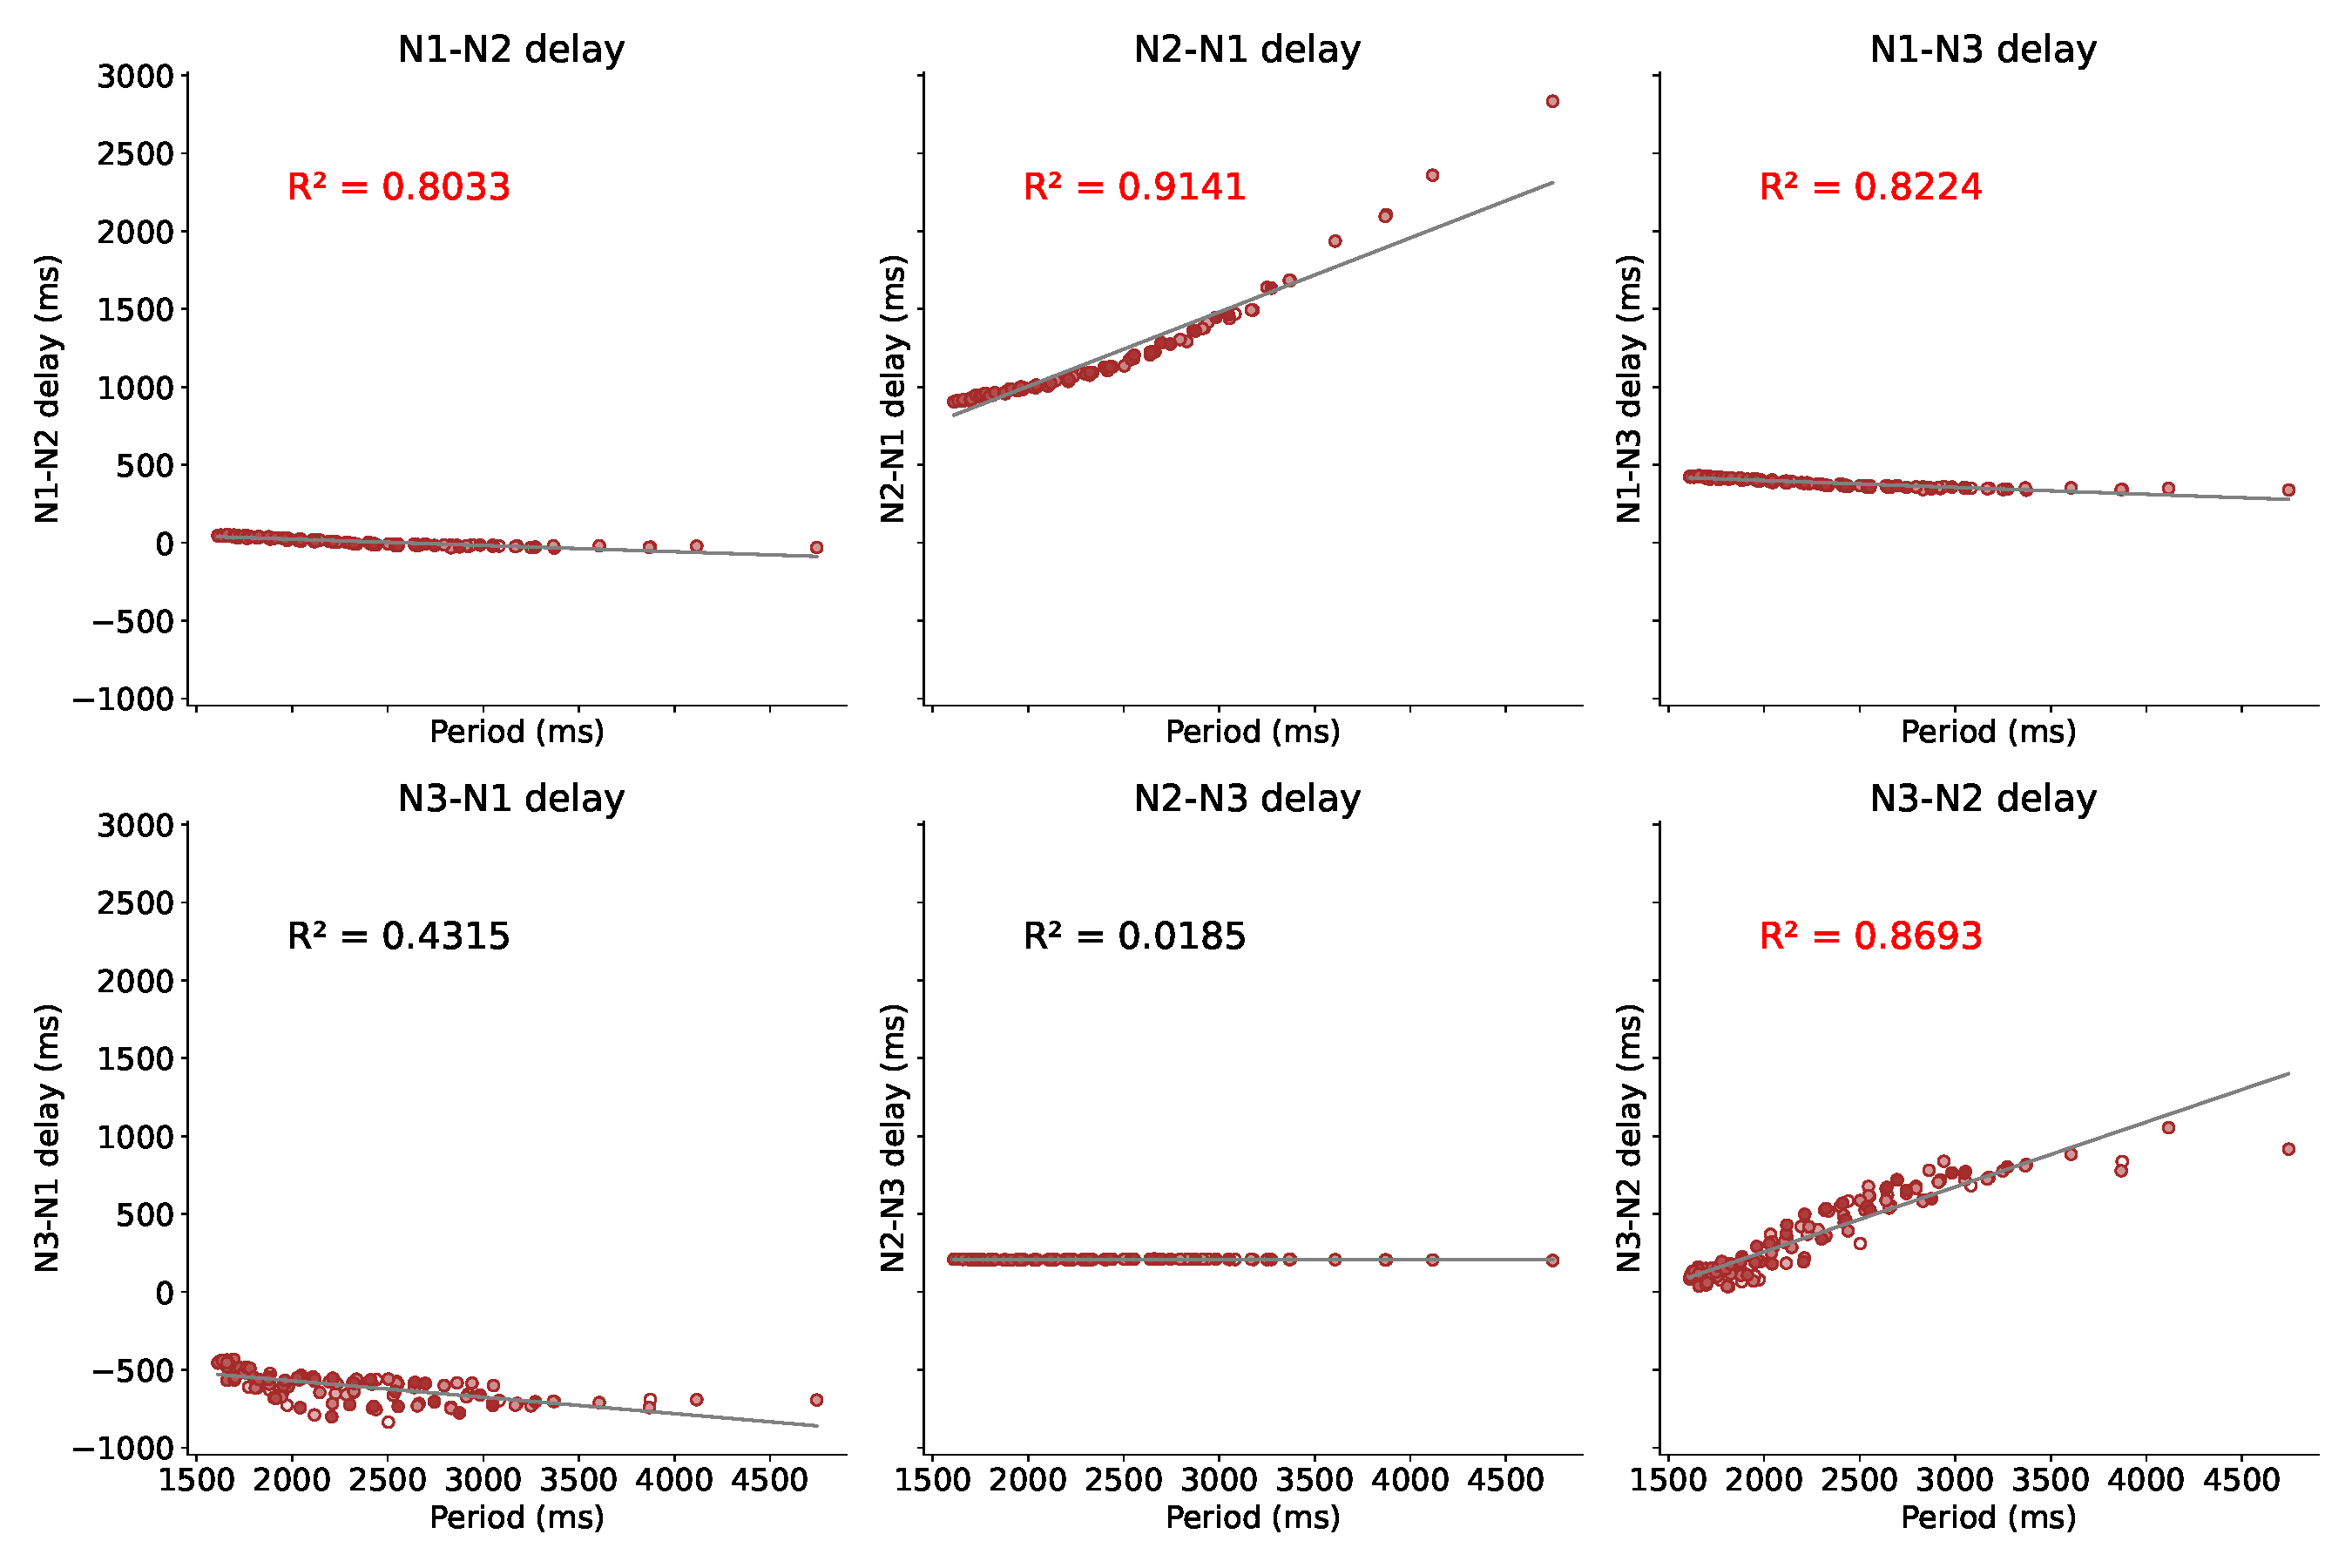
\includegraphics[width=\textwidth]{invariants/data/MODEL/so_driven/images/3phases/_delays.pdf}
		\end{minipage}
	\end{minipage}
	\caption{\textbf{SO stimulation: }a) Box-plots of the sequence intervals under SO neuron stimulation. b) Interval correlations to Period for SO-driven simulation. First row: Burst duration. Second and third row: Two-neuron intervals. Forth and fifth row: Two-neuron delays.}
	\label{fig:invariant so}
\end{figure}


Figure \ref{fig:invariant so}.a) displays the box-plot representing the distinct interval variability. In this case, we found more intervals showing large variability than in the previous cases. N2v intervals, as it happened in the previous results, show low variability. %, which indicates that period variability is more likely a consequence of N3t and N1M activity.
N1M and N3t neurons show high variability in their burst duration intervals, being N1M even more variable than N3t, as opposed to the previous results when the stimulation was introduced in other cells. All intervals derived from these two neurons have high variability and a similar structure. %Therefore, now the intervals which show low variability are the ones related to N2v. 

% In spite all this, what remains constant from N1M-driven simulation is the variability of the N3-N2 interval, which includes both N1M and N3t burst duration, being N3-N2 the most variable one, and the closest to the period variability.%distribution

% Since in this case there are more neurons showing high variability, we should expect finding more correlations when plotting each interval against the period.  ***también deberíamos quitar redundancia aquí***
% Hence, as it happened in the previous results, all intervals related to N3t show dynamical invariants, but this time they are also present in the ones related with N1M, which show a high variability. 
% the intervals with more variability and, thus, those that had a more similar variability structure to the period, were the ones that showed dynamical invariants%(a highest linear relation to the period)


Figure \ref{fig:invariant so}.b) displays the corresponding correlation analysis between all intervals and the period. %In this case, as it happens in the box-plot, there are found different results
In this case, we found correlations in the same intervals as before: N2-N1, N3-N1, N3-N2 intervals and N2-N1 delay; which are the intervals related to N3t burst duration. However, under SO stimulation,  N1-N2, N1-N3 intervals were also highly correlated to the period. Even the correlation for N3-N2 delay considerably increased in relation to the other stimulation conditions. These intervals are the ones related to N1M neuron activity, and were also the most variable ones.  These results reproduce the experimentally analyzed effects set out in \parencite{Elliott1991}, when rhythm and variability was induced by injecting current into a living SO neuron.

%Furthermore, it is important to notice that N3-N1 delay is negative again ****por qué es importante si es lo mismo que antes****. As it happened in N3t-driven simulation, this means there is a constant overlapping between N3 and N1 in each cycle, i.e. N3t burst interval is coming earlier. This can be also appreciated in boxplot, since this interval is represented below 0. 

Compared to the N1M and N3t stimulation results, there is another difference when driving the rhythm with SO: burst duration is much shorter, so the period and the rest of intervals are consequently smaller. Therefore, when driving the rhythm by SO, the period variability seems to arise from both N3t as well as by N1M. 
%the model produces a rhythm where the information about period duration seems to be carried by N3t as well as by N1M. 



\subsection{Time intervals relations cycle-by-cycle beyond period}
We saw so far the sequential dynamical invariants in terms of strong linear relationships between the distinct intervals in a cycle and the period, however, studying the relations between all possible combinations between intervals can also show interesting information about the temporal variability distribution in the ongoing activity. In Figs \ref{fig:model n1m stimulation pairplot} to \ref{fig:model so stimulation pairplot} there is a representation of all these combinations of the defined intervals for the three scenarios of induced variability (current in N1M, N3t or SO) showed in this section. In this extended representation of the relations cycle-by-cycle we can see that there are more intervals presenting strong linear relations, besides of the periods. Some of them are intervals that are contained in others, as the case of N1-BD and N1-N2 interval and have similar durations, and so they are more likely to have a strong linear relation between them. However, there are other intervals that, as it is the case of the period, although they share part of the time-interval, they are not correlated, since they are not the variable part, as it is the case of N2-BD with N1-N2. This disctintion can help disect the source of variability and its distribution when an interval is related to the period. Also, the further study of linear relation between some intervals (as N1-BD and N3-BD) that do not share time-interval, can show significant information about the ongoing activity cycle-by-cycle. This representation can also show non-linear relation between the intervals as we can see in some plots in the case of SO (Fig. \ref{fig:model so stimulation pairplot}), observed in the pyloric CPG in modeling and experimental scenarios \parencite{berbel_emergence_2024}.

\begin{figure}[htbp]
	\centering
	\includegraphics[width=\textwidth]{./invariants/data/MODEL/n1m_driven/images/3phases/output_pairplot.pdf}
	\caption{\textbf{N1M stimulation}: Pairplot with all possible combination between time intervals within a cycle.}
	\label{fig:model n1m stimulation pairplot}
\end{figure}
 
\begin{figure}[htbp]
	\centering
	\includegraphics[width=\textwidth]{./invariants/data/MODEL/n3t_driven/images/3phases/output_pairplot.pdf}
	\caption{\textbf{N3t stimulation}: Pairplot with all possible combination between time intervals within a cycle.}
	\label{fig:model n3t stimulation pairplot}
\end{figure}

\begin{figure}[htbp]
	\centering
	\includegraphics[width=\textwidth]{./invariants/data/MODEL/so_driven/images/3phases/output_pairplot.pdf}
	\caption{\textbf{SO stimulation}: Pairplot with all possible combination between time intervals within a cycle.}
	\label{fig:model so stimulation pairplot}
\end{figure}

%
\subsection{Comparison with two-phase intervals}
During this section we analyzed the sequential dynamical invariants in for three phases, bur we can also define the intervals for two phases of the neurons, taking as reference for example, N1 and N3. This is the case in the work by \cite{elices_robust_2019}, and in the following section we will also use two phases for some of the recordings were the N2 phase was not possible to characterize out of the intracellular recordings. In Figure \ref{fig:invariant n1m model 2 phases} there is a comparison of the linear relations and different intervals conforming the sequence when the references are in N1, N2 and N3 (as we have shown so far) or only for N1 and N3.

When we only consider two phases, we have less possible combinations and the time-intervals that would correspond to the third neuron are contained in the resulting ones. For example as we can see in Fig. \ref{fig:invariant n1m model 2 phases}a), N2N3 delay would be represented by N1N3 delay; N2 burst duration is included in the N2N3 interval. So when analyzing dynamical invariants in two-phase intervals each interval is more informative of the variability constrains cycle-by-cycle. 

\begin{figure}[hbt!]
	\begin{minipage}[b]{0.9\textwidth}
		\raggedleft
		\begin{minipage}[b]{0.53\textwidth}
			\raggedleft
			\begin{overpic}[width=\textwidth]{methods-paper-modelo/Intervals_figure_complete.png}
				\put(0,40){\large\textbf{a)}}
			\end{overpic}
%			\includegraphics[width=\textwidth]{methods-paper-modelo/Intervals_figure_complete.png}
		\end{minipage}
		\centering 
		\begin{minipage}[b]{0.3\textwidth}
			\centering
			\includegraphics[width=\textwidth]{methods-paper-modelo/Intervals_figure_complete_2_phases.png}
		\end{minipage}	
	\end{minipage}\\
	\begin{minipage}[b]{0.53\textwidth}
		\centering
		\begin{minipage}[b]{\textwidth}
			\centering
			\begin{overpic}[width=\textwidth]{invariants/data/MODEL/n1m_driven/images/3phases/_durations.pdf}
				\put(0,35){\large\textbf{b)}}
			\end{overpic}
		\end{minipage}\
		\begin{minipage}[b]{\textwidth}
			\centering
			\includegraphics[width=\textwidth]{invariants/data/MODEL/n1m_driven/images/3phases/_intervals.pdf}
		\end{minipage}\
		\begin{minipage}[b]{\textwidth}
			\centering
			\includegraphics[width=\textwidth]{invariants/data/MODEL/n1m_driven/images/3phases/_delays.pdf}
		\end{minipage}
	\end{minipage}
	\begin{minipage}[b]{0.45\textwidth}
		\centering
		\begin{minipage}[b]{\textwidth}
			\centering
			\begin{overpic}[width=\textwidth]{invariants/data/MODEL/n1m_driven/images/2phases/_durations.pdf}
				\put(0,50){\large\textbf{c)}}
		\end{overpic}
		\end{minipage}\
		\begin{minipage}[b]{\textwidth}
			\centering
			\includegraphics[width=\textwidth]{invariants/data/MODEL/n1m_driven/images/2phases/_intervals.pdf}
		\end{minipage}\
		\begin{minipage}[b]{\textwidth}
			\centering
			\includegraphics[width=\textwidth]{invariants/data/MODEL/n1m_driven/images/2phases/_delays.pdf}
		\end{minipage}
	
		\vspace{50pt}
	\end{minipage}
	\caption{a) Representation of the intervals for each cycle when considering three or two phases (left and right, respectively). b) Interval correlations to period for SO-driven simulation for 3 phases. First row: Burst duration. Second and third row: Two-neuron intervals. Forth and fifth row: Two-neuron delays (Data shown in Fig. \ref{fig:invariant n1m}). c) Interval correlations to period for N1M-driven simulation for 2 phases. First row: Burst duration. Second row: Two-neuron intervals. Third row: Two-neuron delays. For b) and c) the linear relationships are quantified by the $R^2$ values of the regression.}
	\label{fig:invariant n1m model 2 phases}
\end{figure}


\clearpage
\newpage

\section{Experimental results in \textit{Lymnaea Stagnalis}}
\label{sec:experimental sussex}
When studying temporal structures in neural dynamics, the definition of the time references is a key first point. In the computational analysis in the previous section, the time reference to define the intervals were first and last spike of each burst. In that case, as in the case of interneurons in \textit{C. maenas} the CPG phases are directly related with the bursting activity of these neurons and the burst can be consistently defined by the first and last spike. However, in the case of \textit{Lymnaea stagnalis}, activity is usually characterized using recordings from both interneurons and motoneurons \parencite{elliott_interactions_1985, staras_pattern-generating_1998, benjamin_distributed_2012}. This leads to the need of a combination of burst references to characterize the phases of the CPG based on the time intervals cycle by cycle. Thus, for this analysis, we will consider the three phases in the CPG, protraction, rasp and swallow, that are associated mainly to N1M, N2v and N3t neurons. Since it is not always possible to record those neurons at the same time (specially N2v that is in the ventral side), we will define them by a combination of interneurons and motoneurons following their activity at each phase. For example, in Figure \ref{fig:example lymnaea phases recording} the three phases in the  CPG are marked by a colored background over the recording, note how it can be delimited by the neurons in the circuit but some of the motoneurons cover several phases, as it is the case of B4 in panel a) or B3 in panel b). Also phases can be defined by the first and last spike, as it is the case for phase N3 and neuron B8, but in other cases as the phase N2, the reference is the hyperpolarization of some neurons, such as the strong inhibition visible in neuron B5 in panel b). Also, depolarization of some neurons carry relevant information, since for example in the case of B1 the "bumps" visible represent the N1 phase, by the connection between N1M and B1. Therefore, to characterize the time sequences in the feeding CPG, we need compound reference from several neural recordings that can be summarized as in Table \ref{table:cpg ref intervals}. Note that, although different time references must be taken into account when reaching conclusions about the time-interval restrictions and analysis, all possible intervals conforming each cycle between the neurons are taking into account in this analysis (see \ref{subsec:intervals}), so the restrictions and analysis are still relevant.

\begin{table}[htb!]
	\centering
	\begin{tabular}{cl|l|l}
		\multicolumn{1}{l}{}                                 & \multicolumn{1}{c|}{\textbf{N1-Protraction}} & \multicolumn{1}{c|}{\textbf{N2-Rasp}} & \multicolumn{1}{c}{\textbf{N3-Swallow}} \\ \hline
		\multicolumn{1}{c|}{\multirow{3}{*}{\textbf{Start}}} & Last spike of N3t/B3                         & Inhibition of B5                      & First spike of B8                       \\
		\multicolumn{1}{c|}{}                                & Depolarization or first spike in B1          &                                       &                                         \\
		\multicolumn{1}{c|}{}                                & First spike in B6                            &                                       &                                         \\ \hline
		\multicolumn{1}{c|}{\multirow{2}{*}{\textbf{End}}}   & Last spike of B5                             & First spike of B8                     & Last spike of N3t/B3                    \\
		\multicolumn{1}{c|}{}                                & Hyperpolarization in B1 or B6                &                                       &                                        
	\end{tabular}
	\caption{Time reference boundaries for the three phases in the feeding CPG}
	\label{table:cpg ref intervals}
\end{table}



\begin{figure}[bth!]
	\centering
	\begin{minipage}[b]{\textwidth}
		\makebox[0pt][l]{\hspace*{-130pt}\text{a)}}\\
		\centering
		\includegraphics[width=0.9\textwidth]{img/invariants/example_phases_1.pdf}
	\end{minipage}
	\vspace{20pt}
	\begin{minipage}[b]{\textwidth}
		\makebox[0pt][l]{\hspace*{-130pt}\text{b)}}\\
		\centering
		\includegraphics[width=0.9\textwidth]{img/invariants/example_phases_2.pdf}
	\end{minipage}
	\caption{Delimitation of phases in the feeding CPG of \textit{Lymnaea stagnalis} based on different recordings. Panel a) intracellular recordings for motoneurons B4,B3,B1 and B8 and the interneuron N1M. Phases are delimited by N1M and B1, that have the same activation time for phase N1, the inhibition of N1M and the start of the depolarization in B8 for phase N2 and the first and last spike of burst B8 for phase N3. Panel b) intracellular recordings for motoneurons B3,B4,B5, B1 and B8. Phases are delimited by B1 depolarization for phase N1, the strong inhibition of B5 for phase N2 and the fisrt and last spike of burst B8 for phase N3.}
	\label{fig:example lymnaea phases recording}
\end{figure}

Another key point in the study of the feeding CPG of \textit{L. stagnalis} is that the generation of the rhythm is a combined action of different cells \cite{benjamin_distributed_2012}, not only interneurons but also motoneurons have a role in the activation \parencite{staras_pattern-generating_1998} and modulatory neurons in the buccal and cerebral ganglia are involved in the rhythm. All these factors affect the rhythm and thus the neuronal sequential activation and how variability is distributed among the different intervals cycle by cycle. Also, not all the neurons are involved every time the rhythm is active, and that gives also information about the different contexts in which the rhythm is taking part. For example, the rhythm can be activated by the presence of food or sucrose stimulation, in which case the animal needs to initiate the activity and ingest food, the rhythm is started by the stimulation of the lip nerve that also stimulates N1M. Also, even at the absence of food but when the animal is hungry, the CPG can be activated, in this case with a strong role of N3t as modulator. The modulation of the rhythm is also a key aspect and modulatory neurons as SO or CV1a control the rhythm after its initiation, showed to have distinct alternative roles in the activity \parencite{kemenes_multiple_2001}. 

\begin{figure}[bth!]
	\centering
	\includegraphics[width=\textwidth]{img/invariants/distributed_benjamin_2012.pdf}
	\caption{Representation of the distributed system of the feeding CPG. Dots indicate inhibitory chemical synapses, bars excitatory chemical synapses and resistor symbols electrotonic (electrical) synapses. Colors indicate the function of the neuron classified in modulatory or initiator (orange and yellow, respectively) and the three phases protraction, rasp and swallow (green, blue and red, respectively). From left to right food detection represented by Lips that stimulate CGC, SO CBIs and N1M neurons and initiate the rhythm. The ongoing activity is then modulated by those neurons but also by OC neurons and N1 and N3t neuron. Some examples of motor neurons are represented on the right side of the panel, associated to each feeding phase. This figure was adapted from Panel C from Figure 1 in \cite{benjamin_distributed_2012} (work under license \href{http://creativecommons.org/licenses/by/2.0}{Creative Commons Attribution})}
	%	Synaptic connectivity and functions of neurons in the feeding circuit. Modulatory function is indicated by yellow and initiating function by orange. CPG interneurons and motoneurons active during the three phases of the feeding rhythm are indicated by green (P = protraction), blue (R = rasp) and red (S = swallow). Neurons labeled with two colors have two functions. Dots indicate inhibitory chemical synapses, bars excitatory chemical synapses and resistor symbols electrotonic (electrical) synapses. This figure emphasizes the point that many of the neurons have more than function in the feeding network. See Abbreviations for all definitions of neuron types.
	\label{fig:feeding distribution}%
\end{figure}

%Benjamin2012    One of the central controllers of
%spontaneous feeding is the N3t CPG interneuron and
%this cell is involved in mediating the effects of hunger
%and satiety. As was described earlier, the N3ts fire toni-
%cally to inhibit the N1M cells and the rate of this tonic
%activity determines the level of activity in the whole feed-
%ing CPG. By comparing the rates of firing in isolated
%ganglia it was found that the N3t firing frequency was
%higher in satiated compared with starved snails and that
%this was inversely correlated to the frequency of sponta-
%neously fictive feeding cycles [4]. 

%kemenes 2001
%CV1a by modulating motoneuron burst duration and SO by setting the frequency of the ongoing rhythm

In this section we will analyze and describe different examples of experiments for the isolated ganglia with intracellular recordings under: spontaneous activity, SO-driven activity spontaneous and induced, medium lip nerve stimulation induced activity and CV1a-driven induced activity.



\subsection{Invariants in spontaneous activity}
The spontaneous activity here refers to intracellular recordings of the buccal ganglia after the isolation of the CNS with no chemical or electrical induced stimulation. In that case, since the CPG is able to maintain the activity in an autonomous manner, it keeps the motor activity as if the CNS was not isolated. In this case, although the characterization of the sequential dynamical invariants can be done, their possible functionality association is more complicated, since the context of the movement origin is lost. The study of these sequential restriction in artificial stimulation context can help classify this spontaneous activity, even when the rest of the system is not available. 

Here we analyze three examples of the spontaneous activity, 

\paragraph{Spontaneous Activity Example 1}
N1 phase was analyzed from B1 activity (bursting and depolarization); N2 phase was analyzed from B5 hyperpolarization, which has a strong inhibition from N2v; N3 phase was analyzed from the bursting activity of B8, that replicates the N3t duration. 

\begin{figure}[htbp]
	\centering
	\includegraphics[width=0.9\textwidth]{./invariants/data/SUSSEX/prep2/images/3phases/panel_with_intervals.pdf}
	\caption{\textbf{Spontaneous case 1}: Panel of intervals distribution and dynamical invariants for the three phases in the CPG for spontaneous activity.}
	\label{fig:prep2 invariants}
\end{figure}

\begin{figure}[htbp]
	\centering
	\includegraphics[width=\textwidth]{./invariants/data/SUSSEX/prep2/images/3phases/panel_with_pairplot.pdf}
	\caption{\textbf{Spontaneous case 1}: Panel of intervals distribution and dynamical invariants for the three phases in the CPG for spontaneous activity.}
	\label{fig:prep2 pairplot invariants}
\end{figure}


%\begin{figure}[htbp]
%	\centering
%	\includegraphics[width=0.9\textwidth]{./invariants/data/SUSSEX/prep2/images/2phases/panel_with_intervals.pdf}
%	\caption{\textbf{Spontaneous case2}: Panel of intervals distribution and dynamical invariants for two phases in the CPG for spontaneous activity.}
%	\label{fig:prep2 2phase invariants}
%\end{figure}
%
%\begin{figure}[htbp]
%\centering
%\includegraphics[width=0.9\textwidth]{./invariants/data/SUSSEX/prep2/images/2phases/panel_with_pairplot.pdf}
%\caption{\textbf{Spontaneous case2}: Panel of intervals distribution and dynamical invariants for two phases in the CPG for spontaneous activity.}
%\label{fig:prep2 2phase invariants pairplot}
%\end{figure}

\paragraph{Spontaneous Activity Example 2}
N1 phase was analyzed from B1 activity (bursting and depolarization); N2 phase was analyzed from B1 hyperpolarization, which has a strong inhibition from N2v; N3 phase was analyzed from the bursting activity of B8, that replicates the N3t duration. 
Since the reference for N2 here coincides with N1 reference, we display here only the intervals corresponding to N1 and N3 phases, since the intervals that correspond to 3 phases, such as N1-N2 delay or N2-N3 delay, either are already represented in the defined intervals or have a duration close to 0 ms.

\begin{figure}[htbp]
	\centering
	\includegraphics[width=0.9\textwidth]{./invariants/data/SUSSEX/prep3/images/2phases/panel_with_intervals.pdf}
	\caption{\textbf{Spontaneous case 2}: Panel of intervals distribution and dynamical invariants for two phases in the CPG for spontaneous activity.}
	\label{fig:prep3 2phases invariants}
\end{figure}

\begin{figure}[htbp]
	\centering
	\includegraphics[width=0.9\textwidth]{./invariants/data/SUSSEX/prep3/images/2phases/panel_with_pairplot.pdf}
	\caption{\textbf{Spontaneous case 2}: Panel of intervals distribution and dynamical invariants for two phases in the CPG for spontaneous activity.}
	\label{fig:prep3 2phases invariants pairplot}
\end{figure}

%\begin{figure}[htbp]
%	\centering
%	\includegraphics[width=0.9\textwidth]{./invariants/data/SUSSEX/prep3/images/3phases/panel_with_intervals.pdf}
%	\caption{\textbf{Spontaneous case3}: Panel of intervals distribution and dynamical invariants for the three phases in the CPG for spontaneous activity.}
%	\label{fig:prep3 invariants}
%\end{figure}
%
%\begin{figure}[htbp]
%	\centering
%	\includegraphics[width=0.9\textwidth]{./invariants/data/SUSSEX/prep3/images/3phases/panel_with_pairplot.pdf}
%	\caption{\textbf{Spontaneous case3}: Panel of intervals distribution and dynamical invariants for the three phases in the CPG for spontaneous activity.}
%	\label{fig:prep3 invariants pairplot}
%\end{figure}


\paragraph{Spontaneous Activity Example 3}
N1 phase was analyzed from B1 activity (bursting and depolarization); N2 phase was analyzed from B5 hyperpolarization, which has a strong inhibition from N2v; N3 phase was analyzed from the bursting activity of B8, that replicates the N3t duration. 

\begin{figure}[htbp]
	\centering
	\includegraphics[width=0.9\textwidth]{./invariants/data/SUSSEX/prep1/images/3phases/panel_with_intervals.pdf}
	\caption{\textbf{Spontaneous case 3}: Panel of intervals distribution and dynamical invariants for the three phases in the CPG for spontaneous activity.}
	\label{fig:prep1 invariants}
\end{figure}


\begin{figure}[htbp]
	\centering
	\includegraphics[width=\textwidth]{./invariants/data/SUSSEX/prep1/images/3phases/panel_with_pairplot.pdf}
	\caption{\textbf{Spontaneous case 3}: Panel of intervals distribution and dynamical invariants for the three phases in the CPG for spontaneous activity.}
	\label{fig:prep1 invariants pairplot}
\end{figure}

%
%\begin{figure}[htbp]
%	\centering
%	\includegraphics[width=0.9\textwidth]{./invariants/data/SUSSEX/prep1/images/2phases/panel_with_intervals.pdf}
%	\caption{\textbf{Spontaneous case1}: Panel of intervals distribution and dynamical invariants for two phases in the CPG for spontaneous activity.}
%	\label{fig:prep1 2 phases invariants}
%\end{figure}
%%
%\begin{figure}[htbp]
%	\centering
%	\includegraphics[width=0.9\textwidth]{./invariants/data/SUSSEX/prep1/images/2phases/panel_with_pairplot.pdf}
%	\caption{\textbf{Spontaneous case1}: Panel of intervals distribution and dynamical invariants for the two phases in the CPG for spontaneous activity.}
%	\label{fig:prep1 2 phases invariants pairplot}
%\end{figure}




\subsection{Invariants in SO driven activity}
\paragraph{1. Spontaneous SO modulation recording}
% Nota: datos de preparación 4 en la detección está solo n1m y b8, las fases son N1 y N3. 
 
\begin{figure}[htbp]
	\centering
	\includegraphics[width=0.9\textwidth]{./invariants/data/SUSSEX/prep4_so_driven_2/images/panel_with_intervals.pdf}
	\caption{\textbf{Spontaneous SO neuron driven}: Panel of intervals distribution and dynamical invariants for the two phases in the CPG for spontaneous activity driven by SO neuron.}
	\label{fig:so spontaneous invariants}
\end{figure}

\begin{figure}[htbp]
	\centering
	\includegraphics[width=0.9\textwidth]{./invariants/data/SUSSEX/prep4_so_driven_2/images/panel_with_pairplot.pdf}
	\caption{\textbf{Spontaneous SO neuron driven}: Panel of intervals distribution and dynamical invariants for the two phases in the CPG for spontaneous activity driven by SO neuron.}
	\label{fig:so spontaneous invariants pairplot}
\end{figure}
 	


\begin{figure}[htbp]
	\centering
	\includegraphics[width=0.9\textwidth]{./invariants/data/SUSSEX/prep4_so_no_driven/images/panel_with_intervals.pdf}
	\caption{\textbf{Spontaneous activity when SO-driven is over}: Panel of intervals distribution and dynamical invariants for the three phases in the CPG for spontaneous activity.}
	\label{fig:no so spontaneous invariants}
\end{figure}
 	 
 
\begin{figure}[htbp]
	\centering
	\includegraphics[width=0.9\textwidth]{./invariants/data/SUSSEX/prep4_so_no_driven/images/panel_with_pairplot.pdf}
	\caption{\textbf{Spontaneous activity when SO-driven is over}: Panel of intervals distribution and dynamical invariants for the three phases in the CPG for spontaneous activity.}
	\label{fig:no so spontaneous invariants pairplot}
\end{figure}
 
\paragraph{2. Stimulated SO recording}


\begin{figure}[htbp]
	\centering
	\includegraphics[width=0.9\textwidth]{./invariants/data/SUSSEX/SO_driven/images/panel_with_pairplot.pdf}
	\caption{\textbf{SO driven stimulation}: Panel of intervals distribution and dynamical invariants for the three phases in the CPG under SO modulatory neuron stimulation.}
	\label{fig:so stimulation pairplot}
\end{figure}



\subsection{Invariants in MLN stimulation driven activity}
The snail's lips are connected to the cerebral ganglia by the MLN (median lip nerves). It is possible to stimulate CPG activity by its stimulation, simulating the initiation of the rhythm in food presence \parencite{staras_electrophysiological_2019}. The data in this recording was stimulated by (4volt 1Hz stim).


\begin{figure}[htbp]
	\centering
	\includegraphics[width=0.9\textwidth]{./invariants/data/SUSSEX/MLN_driven/images/panel_with_intervals.pdf}
	\caption{\textbf{MLN stimulation}: Panel of intervals distribution and dynamical invariants for the three phases in the CPG under MLN Medium Lip Nerve (MLN) stimulation.}
	\label{fig:mln stimulation}
\end{figure}


\begin{figure}[htbp]
	\centering
	\includegraphics[width=0.9\textwidth]{./invariants/data/SUSSEX/MLN_driven/images/panel_with_pairplot.pdf}
	\caption{\textbf{MLN stimulation}:Pairplot of the invariants reset within cycles.}
	\label{fig:mln stimulation pairplot}
\end{figure}


\begin{figure}[htbp]
	\centering
	\includegraphics[width=0.9\textwidth]{./invariants/data/SUSSEX/MLN_driven/images/_output_pairplot_reset.png}
	\caption{\textbf{MLN stimulation}: Panel of intervals distribution and dynamical invariants for the three phases in the CPG under MLN Medium Lip Nerve (MLN) stimulation.}
	\label{fig:mln stimulation reset pairplot}
\end{figure}


\subsection{Invariants in cva1 stimulation driven activity}
CV1a is part of a larger population of CBIs 
%and the complete map of their locations is shown in Figure 3A. https://static-content.springer.com/esm/art%3A10.1186%2F2042-1001-2-4/MediaObjects/13232_2011_20_MOESM3_ESM.jpeg
Sucrose drives rhythmic activity in CBIs activating the feeding circuit by the conection
\paragraph{Example 1}

%\begin{figure}[htbp]
%	\centering
%	\includegraphics[width=0.9\textwidth]{./invariants/data/SUSSEX/CV1a_driven1/images/3phases/panel_with_intervals.pdf}
%	\caption{\textbf{CV1a driven case1}: Panel of intervals distribution and dynamical invariants for the three phases in the CPG under CV1a stimulation.}
%	\label{fig:cv1a 1 3phases}
%\end{figure}
%
%\begin{figure}[htbp]
%	\centering
%	\includegraphics[width=0.9\textwidth]{./invariants/data/SUSSEX/CV1a_driven1/images/3phases/panel_with_pairplot.pdf}
%	\caption{\textbf{CV1a driven case1}: Panel of intervals distribution and dynamical invariants for the three phases in the CPG under CV1a stimulation.}
%	\label{fig:cv1a 1 3phases pairplot}
%\end{figure}

\begin{figure}[htbp]
	\centering
	\includegraphics[width=0.9\textwidth]{./invariants/data/SUSSEX/CV1a_driven1/images/2phases/panel_with_intervals.pdf}
	\caption{\textbf{CV1a driven case1}:Panel of intervals distribution and dynamical invariants for the two phases in the CPG under CV1a stimulation.}
	\label{fig:cv1a 1 2phases}
\end{figure}


\begin{figure}[htbp]
	\centering
	\includegraphics[width=0.9\textwidth]{./invariants/data/SUSSEX/CV1a_driven1/images/2phases/panel_with_pairplot.pdf}
	\caption{\textbf{CV1a driven case1}:Panel of intervals distribution and dynamical invariants for the two phases in the CPG under CV1a stimulation.}
	\label{fig:cv1a 1 2phases pairplot}
\end{figure}



\paragraph{Example 2}


\begin{figure}[htbp]
	\centering
	\includegraphics[width=0.9\textwidth]{./invariants/data/SUSSEX/CV1a_driven2/images/panel_with_intervals.pdf}
	
	\caption{\textbf{CV1a driven case2}: Panel of intervals distribution and dynamical invariants for the two phases in the CPG under CV1a stimulation.}
	\label{fig:cv1a 2 2phases}
\end{figure}


\begin{figure}[htbp]
	\centering
	\includegraphics[width=0.9\textwidth]{./invariants/data/SUSSEX/CV1a_driven2/images/panel_with_pairplot.pdf}
	
	\caption{\textbf{CV1a driven case2}: Panel of intervals distribution and dynamical invariants for the two phases in the CPG under CV1a stimulation.}
	\label{fig:cv1a 2 2phases pairplot}
\end{figure}




\paragraph{Example 3}


\begin{figure}[htbp]
	\centering
	\includegraphics[width=0.9\textwidth]{./invariants/data/SUSSEX/CV1a_driven3/images/panel_with_intervals.pdf}
	\caption{\textbf{CV1a driven case3}: Panel of intervals distribution and dynamical invariants for the two phases in the CPG under CV1a stimulation.}
	\label{fig:cv1a 3 2phases}
\end{figure}



\paragraph{Example 4}

%\begin{figure}[htbp]
%	\centering
%	\includegraphics[width=0.9\textwidth]{./invariants/data/SUSSEX/CV1a_driven4/images/3phases/panel_with_intervals.pdf}
%	\caption{\textbf{CV1a driven case 4}: Panel of intervals distribution and dynamical invariants for the three phases in the CPG under CV1a stimulation.}
%	\label{fig:cv1a 4 3phases}
%\end{figure}
%
%\begin{figure}[htbp]
%	\centering
%	\includegraphics[width=0.9\textwidth]{./invariants/data/SUSSEX/CV1a_driven4/images/3phases/panel_with_pairplot.pdf}
%	\caption{\textbf{CV1a driven case 4}: Panel of intervals distribution and dynamical invariants for the three phases in the CPG under CV1a stimulation.}
%	\label{fig:cv1a 4 3phases pairplot}
%\end{figure}

\begin{figure}[htbp]
	\centering
	\includegraphics[width=0.9\textwidth]{./invariants/data/SUSSEX/CV1a_driven4/images/2phases/panel_with_intervals.pdf}
	\caption{\textbf{CV1a driven case4}: Panel of intervals distribution and dynamical invariants for the two phases in the CPG under CV1a stimulation.}
	\label{fig:cv1a 4 2phases}
\end{figure}

\begin{figure}[htbp]
	\centering
	\includegraphics[width=0.9\textwidth]{./invariants/data/SUSSEX/CV1a_driven4/images/2phases/panel_with_pairplot.pdf}
	\caption{\textbf{CV1a driven case4}: Panel of intervals distribution and dynamical invariants for the two phases in the CPG under CV1a stimulation.}
	\label{fig:cv1a 4 2phases pairplot}
\end{figure}

\subsection{Summary}
\begin{figure}
	\includegraphics[width=\textwidth]{./invariants/styled_table_invariants_r-squared.pdf}
	\caption{Table of $R^2$ values for the linear regression between the period and each interval for all experimental recordings showed in this section.}
	\label{fig:R2 table}
\end{figure}

\begin{figure}
	\includegraphics[width=\textwidth]{./invariants/styled_table_invariants_r-value.pdf}
	\caption{Table of $R$ values for the linear regression between the period and each interval for all experimental recordings showed in this section.}
	\label{fig:R table}
\end{figure}




\section{Characterization of variability in bursting models and its functionality}
\label{sec:model variability}
Bursting dynamics has been extensively studied in a wide variety of neural systems, as it is instrumental for many brain functions, including motor coordination and cognitive performance, and can be related to both healthy and pathological states. Neuronal models in computational neuroscience often reproduce key functional features of their biological counterparts. However, they also present limitations such as their poor ability to mimic the observed intrinsic variability of living neurons, particularly in membrane potential waveforms and in collective adaptive dynamics. Biophysical models typically produce stereotyped fixed membrane potential depolarization and repolarization waveforms, and restricted dynamical flexibility as compared to those observed in experimental recordings. Variability in the activity of living neurons has been proven to play an important role in relevant information processing tasks. We have seen in this chapter, the importance of variability in the presence of sequential dynamical invariants in the bursting activity and the limitations of studying them in a model when the variability is induced by a current ramp stimulation. The variability in models has usually been induced by gaussian noise, but this ignores the importance of the functional variability in the neurons, the observed variability is not only a cause of stochastic alterations but a functional outcome. 

In this section, we will describe this variability characteristics in experimental recordings, not only regarding the sequence time-intervals but also their waveforms. We will compare this variability with that of classical models and models able to produce chaotic activity. 
Figure \ref{fig:lp-pd burst variability} shows examples of the bursting and waveform variability in the intracellular recordings of LP and PD neurons in the pyloric CPG of \textit{Carcinus maenas}. In both neurons, we can appreciate a wide variability in the burst shape and duration, including the variability in the hyperpolarization.

\begin{figure}[hbt]
	\centering
	\begin{minipage}{0.48\textwidth}
		\includegraphics[width=\textwidth]{img/invariants/variability/lp_burst_variability.png}
	\end{minipage}
	\begin{minipage}{0.48\textwidth}
		\includegraphics[width=\textwidth]{img/invariants/variability/pd_burst_variability.png}
	\end{minipage}
	\caption{Example of variability in waveforms from intracellular recordings of the LP and PD neurons in the pyloric CPG}
	\label{fig:lp-pd burst variability}
\end{figure}

Although models can faithfully reproduce the activity and shape of neural models, they usually fail on reproducing the intrinsic and collective variability that we observe in electrophysiological recordings, this is the case for example of \textcite{hodgkin_quantitative_1952} or \textcite{vavoulis_dynamic_2007}, represented in Fig. \ref{fig:model burst no variability}. In that reproduction, although the waveform shape is accurate, the functional variability is hindered, reproducing a tonic and steady bursting activity. 

\begin{figure}[hbt]
	\centering
	\begin{minipage}{0.48\textwidth}
		\includegraphics[width=\textwidth]{img/invariants/variability/GHmodel.png}
	\end{minipage}
	\begin{minipage}{0.48\textwidth}
		\includegraphics[width=\textwidth]{img/invariants/variability/N1Mnovar.png}
	\end{minipage}
	\caption{Example of bursts with no variability in waveforms from model simulation of neuron from \textcite{ghigliazza_minimal_2004b} model in chaotic mode and N1M neuron from \textcite{vavoulis_dynamic_2007} with no ramp stimulation in the CPG circuit. The equations for both models can be found in Secs. \ref{sec:model variability equations} and \ref{sec:CPG model equations}, respectively.}
	\label{fig:model burst no variability}
\end{figure}



In section \ref{sec:CPG model equations}, we saw that variability can be induced by including a current ramp, although it can reproduce the variability, when studying the activity cycle-by-cycle it hinders the functional variability of the spontaneous activity. 


\begin{figure}[hbt]
	\centering
	\begin{minipage}{0.48\textwidth}
		\includegraphics[width=\textwidth]{img/invariants/variability/TN-burst_variability.png}
	\end{minipage}
	\begin{minipage}{0.48\textwidth}
		\includegraphics[width=\textwidth]{img/invariants/variability/n1m_vav_burst_variability.png}
	\end{minipage}
	\caption{Example of variability in waveforms from model simulation of neuron from \textcite{nowotny_probing_2008} model in chaotic mode and N1M neuron from \textcite{vavoulis_dynamic_2007} under current stimulation in the CPG circuit. The equations for both models can be found in Secs. \ref{sec:model variability equations} and \ref{sec:CPG model equations}, respectively.}
	\label{fig:model burst variability}
\end{figure}


Modern experimental techniques involving activity-dependent electrical, optical and chemical stimulation can further unveil and explain functional variability of bursting sequences in a wide variety of nervous systems, it is important to rely on models able to reproduce the intrinsic variability. It will also be relevant for designing associated applications in the context of neurotechnology, artificial intelligence and robotics \parencite{garrido-pena_exploring_2024}. 

%
%In this work, we illustrate that current biophysical neuron models fail to reproduce the intrinsic and collective variability observed in electrophysiological recordings in the nervous system of different animals, and how this hinders the theoretical study of the relevance of sequential neural dynamics. We also assess the solution to this problem in well-known bursting neuron models by identifying possible biophysical and synaptic candidates that can explain the observed variability while sustaining the robustness of the model oscillatory activity. Finally, we discuss the importance of model intrinsic variability in the context of biohybrid circuits built with interacting living and model neurons to evaluate the role of robust sequential neuronal and circuit dynamics in motor function coordination.

%Bursting dynamics has been extensively studied in a wide variety of neural systems, as it is instrumental for many brain functions, including motor coordination and cognitive performance, and can be related to both healthy and pathological states. Much less attention has been paid to the emerging sequential dynamics that underlies many rhythms built with bursting dynamics. Neural bursting activity provides robust temporal references to define time intervals that build sequences that repeat themselves, frequently at different time scales. The study of the variability of sequence time intervals is relevant to understand the balance between robustness of the order of the neural sequence and the flexibility in timing and duration required for the coordination of specific neural functions. The characterization of time intervals underlying bursting sequences has recently yielded the discovery of sequential dynamical invariants in the form of robust cycle-by-cycle relationships among specific intervals that coexist with other intervals whose variability remains unrelated. Sequential dynamical invariants have been proposed to underlie the dynamical coordination in motor circuits that produce rhythmic movements.  

%In this work we expose, reproduce and explain the variability observed in sequential neural bursting dynamics using a combination of experiments, sequence interval data characterization tools and computational models. Our experimental analysis shows that sequential dynamical invariants only exist if sufficient variability is present, and they can be linked to asymmetrical circuit topologies and multiple synaptic timescales. Traditional bursting neural models lack the observed experimental variability but can nevertheless display sequential dynamical invariants from external perturbations or an adequate combination of intrinsic neuron and synaptic dynamics. Modern experimental techniques involving activity-dependent electrical, optical and chemical stimulation can further unveil and explain functional variability of bursting sequences in a wide variety of nervous systems, and to design associated applications in the context of neurotechnology, artificial intelligence and robotics.  
%
%Additional information 
%
%We characterized the activity of bursting neural sequences in two distinct Central Pattern Generator (CPG) circuits (Lymnaea Stagnalis and Carcinus maenas) using long intracellular and extracellular electrophysiological recordings and in their corresponding conductance-based models. We addressed both intrinsic and extrinsic variability with control recordings and perturbations induced by electrical, chemical, optical and biohybrid circuits composed of living and model neurons. We found that robust sequences coexisted with a wide variability in cycle-by-cycle periods and intervals constituting the sequence (see panel A in Fig. 1). We characterized the variability in waveform (panels B-D) and time intervals defined from the beginning and the end of the bursting activity (panels E-F). Specific cycle-by-cycle sequence intervals displayed strong linear (marked with purple asterisks in panels E-F) or nonlinear relations indicating dynamical constraints to the sequential coordination while others had unrelated variability allowing flexibility in timing and duration. Our model analysis showed that invariants emerged when the synaptic mechanisms allow the propagation of the variability through nonsymmetrical mechanisms and rich transient neuronal dynamics. We have developed protocols and analysis tools that have a general use to expose and characterize dynamical invariants in a wide variety of nervous systems, which will serve to validate the universality of this phenomenon and to link it to functionality and healthy and pathological states, including novel neurotechnology design. 




\section{Transformation of sequential intervals into effective robot movement}
\label{sec:robot}
To validate the importance of the balance between robustness and flexibility in  CPG circuits, as provided by the cycle-by-cycle dynamical invariants present in the dynamics discussed in this chapter, we include in this section a validation experiment for the translation of dynamical invariants into an effective motor locomotion in a Functional-Living-Circuit-Hybrot (FLC-Hybrot) \parencite{amaducci_hybrid_2020,amaducci_controlling_2021,soetard_dynamical_2023}. The combination of models, novel tools and experimental approaches has proven its effectiveness in revealing and exploring features of neural dynamics \parencite{szucs_interacting_2000,chamorro_generalization_2012,reyes-sanchez_automatized_2023}. In this first step into the applications in robotics of the variability time constrains found in CPGs, we built an hexapod robot whose legs performed oscillatory activity to move forward. The period and amplitude of these oscillations were determined by the sequential cycle-by-cycle activity of the CPG neurons recorded from the living preparation and sent online to the robot. At the same time, the hybrot included a light sensor and sent feedback information regarding the light conditions around it back to the neural circuit in the form of an electrical current. These stimuli modified the behavior of the cells, resulting in a change of the hybrot locomotion, preserving always the required motor coordination, and therefore forming a real-time closed-loop interaction among living and electronic components (Figure \ref{fig:robot_results_summary} shows a summary of these interactions). The goal of the FLC-Hybrot is to demonstrate that a dynamical principle of the functional living circuit can be used to autonomously coordinate the locomotion with sensory feedback from the robot. In our case, we used the presence of dynamical invariants in the form of robust relationships between the time intervals that build the cycle-by-cycle activity of the neurons of the pyloric CPG in \textit{Carcinus maenas}, which are sustained under any circumstance, even when there are external inputs to the circuit, to modulate the behavior of the robot. Section \ref{sec:robot setup} provided a detailed description of the experimental setup for the hybrot. 

\begin{figure}[hbt!]
	\begin{center}
		% \includegraphics[width=\linewidth]{images/robot/robot_results_summary}
		\includegraphics[width=\textwidth]{img/invariants/robot/Figure1_experiment_design_v1.png}
	\end{center}
	\caption{Representation of the FLC-Hybrot paradigm design. Neural dynamics from a functional living CPG circuit are recorded online and used to coordinate the robot movement in real-time. Activity from the PD neuron is recorded intracellularly (green trace), while the LP bursts are extracted from the nerve's extracellular signal (blue trace). This robot walks through a trial track with interspersed light and shadow regions. When the robot's light sensor detects that it is located under a shadow, it sends feedback current to the living circuit. CPG dynamics change as a reaction to the injected current, thus modifying the robotic locomotion. The following video shows an example of this experiment \url{https://youtu.be/ny2dJGbG8lo}.}
	\label{fig:robot_results_summary}
\end{figure}


To validate the adequate locomotion of the FLC-Hybrot when driven by the pyloric CPG online behavior, as well as the living circuit real-time adaptation to the injected feedback, we performed a set of experiments employing a 1.5 meters long trial track. Along this surface there were interspersed segments of lights and shadows. This configuration caused the FLC-Hybrot to alter its behavior several times during the experiment due to the injection of current into the PD neuron when it walked under a shadow. The current injected in the cell in a shadow section varied from one experiment to another, according to the neurons response to the stimuli. No current was injected when the robot was located on a luminous area. The following video illustrates one of such experiments \url{https://youtu.be/Dltec7TeGso}.

\begin{figure}[hbt!]
	\begin{center}
		\includegraphics[width=0.8\linewidth]{./img/invariants/robot/robot_results_validation}
	\end{center}
	\caption{Flexible hybrot adaptation to environmental changes when noticed by the robot sensors and associated coordinated locomotion. When the robot entered a shadow section, it sent sensory feedback to the living CPG in the form of positive electrical current (red trace). Blue and green traces are recordings of the extracellular and intracellular (PD neuron) activity of the circuit and display the change caused by the feedback current injection in the PD neuron, slowing down the CPG rhythm. The oscillatory movement of the robot legs is represented in the brown trace and it can observed that a variation in the CPG rhythm leads to a change in the robotic locomotion, modifying both the period and the amplitude of the oscillation. 
		%This effect can be seen more clearly in the bottom panel, where both the LP neuron instantaneous bursting period (blue) and the robot legs oscillation period (brown) are plotted together, showing how the latter is modulated by the former.
	}
	\label{fig:robot_results_validation}
\end{figure}

Figure \ref{fig:robot_results_validation} shows the results for one of these tests. We observe a change in the neural activity when -0.6nA current is inserted into the PD neuron, causing the CPG rhythm to slow down while also modifying the PD neuron membrane's potential amplitude. This change is immediately reversed as soon as the current goes back to zero, restoring its previous behavior. Concerning the robot's locomotion, a variation in the legs' oscillation is observed just after the neurons alter their activity. Despite the successive changes in the amplitude and period of its legs' oscillation, the FLC-Hybrot maintained a coordinated and effective locomotion during the whole experiment. 

We know that in the pyloric CPG there is a sequential dynamical invariant, in the form of a linear relation between the LP neuron period and the LPPD interval. These are the intervals used to modulate the amplitude and period of the legs oscilation in the robot. This constrain was effectively transferred to the robot locomotion. Figure \ref{fig:robot_results_invariant} shows a comparison between the living CPG and the robot dynamical invariant, with the later reaching an $R^2$ correlation of 0.87 despite the lack of precision of its servomotors. It displayed the same correlation between its legs oscillation period and amplitude, which were modulated by the two previous temporal intervals. The methodological details for the legs tracking to characterize the effective transfer of the invariants can be found in \textcite{swarc_realtime_2023}.

\begin{figure}[hbt!]
	\begin{center}
		\includegraphics[width=\linewidth]{./img/invariants/robot/robot_results_invariant}
	\end{center}
	\caption{\textbf{Left:} dynamical invariant present in the living CPG activity during the validation test, represented as a cycle-by-cycle linear relation between the LP neuron bursting period and the LPPD interval. \textbf{Right:} dynamical invariant present in the FLC-Hybrot locomotion during the validation test, represented as a cycle-by-cycle linear relation between its legs' oscillation period and amplitude. The dynamical invariant property is effectively translated from the living CPG to the robot locomotion, encoded as: Robot period = LP period, Robot amplitude = LPPD interval * factor.}
	\label{fig:robot_results_invariant}
\end{figure}

This hybrot scenario can help simulate context change situations in which the CPG rhythm is modulated by external factors and there is a change of variability reflected in the relations between the cycle-by-cycle intervals. The reproduction of biological dynamics with preserved coordination time constraints can have strong implications in autonomous robot locomotion, and also in neurorehabilitation technologies. Under the scope of sequential dynamical invariants,  coordination rules are not imposed as conditional commands but autonomously emerge from the intrinsic sequential dynamics.

\section{Discussion}
In this chapter, we studied the sequentially analyzing the bursting activity of the feeding CPG in \textit{L. stagnalis}. As discussed before, this CPG is ideal for this kind of study due to their ability to maintain a robust sequential activation and still present a high flexibility to adapt to changes in the context. Also, the bursting activity provides clearer references than in other more complex circuits. 

In this system addressed the characterization of the intervals building up the rhythmic sequence in this system with model simulations and also in experimental intracellular recordings. We tested the presence of sequential dynamical invariants in the form of linear relationships between the sequence intervals and the cycle period of the rhythm following the experimental results that we reported in \textcite{elices_robust_2019} for the crustacean pyloric CPG. Most extended studies usually study the averaged variability, masking the information in the relations taking place at each cycle of sequential activations. Taking that into account, here we characterize the variability cycle-by-cycle. 

In the model, we extended the analysis of the reported relations by \textcite{Elliott1991} by characterizing each and every interval building the sequence and relating the strong linear relationships found in specific intervals to the concept of robust sequential dynamical invariants proposed in \textcite{elices_robust_2019} for the coordination of robust yet flexible CPG rhythms. In the simulations, three main cases have been addressed in the analysis: N1M-driven, SO-driven and N3t-driven stimulation. This was based on the two different possibilities of inducing variability in the model according to the results reported in \textcite{vavoulis_dynamic_2007}, as well as with a third neuron stimulation (N3t) which is easily addressable in the model circuit. When variability arises by the stimulation of N1M, the results are rather similar to the ones obtained stimulating N3t. Strong linear correlations to the period, i.e.,  dynamical invariants, are present mainly in all intervals related to N3 phase, since these are the ones with cycle-by-cycle variability related to the period variability.  

We also show the redistribution of variability that takes place when the stimulation is applied on SO. In this scenario more intervals presenting large variability than in the other stimulation protocols are found. This is due to the specific variability of N1M and N3t burst duration, since in this case the largest influence on the period seems to come not only from N3t but also from N1M. Hence, consequently to the variability analysis, different linear relationships are found involving all intervals related to N3 and N1 phases. The intervals unrelated to the period are the ones associated with N2 phase, which is also the least variable entity in the circuit. 

These results reproduce and extend the ones discussed in \textcite{vavoulis_dynamic_2007} and \textcite{Elliott1991}. It is interesting to highlight the differences in the results when the period is driven by N1M/N3t or SO. When the variability is induced in N1M/N3t, N3t is still able to inhibit the N1M neuron carrying the main variability, while SO is adapting to both. However, when SO is the neuron being stimulated, since it is connected to N1M by mutual excitation, they are both boosting each other's activity, leading to the higher variability of N1M. Here, N3t must adapt to N1M, which is harder due to the SO constant excitation. For this reason, it was necessary to inject some additional current in N3t in the simulations, which would usually be an input received from the cerebral ganglia. 

Each of the three phases of the rhythm corresponds to a specific motor action: N1 protraction, N2 rasp and N3 swallow. As it is pointed out in \textcite{Elliott1991}, the motor sequence consists of a two-stroke relaxation: protraction and rasp (N1,N2), in charge of moving the radula, and swallowing (N3). In these kind of systems, it is common to find one of them fixed and the other one variable, which in our case is the swallow phase. In this context, SO stimulation can be related to sucrose stimulation \textcite{benjamin_distributed_2012,kemenes_analysis_1994},
this could be related with the increase in N1M variability, since in presence of food, protraction phase may become crucial for an effective food reaching. Thus, there might be now two phases showing more variability in their intervals duration. The discussed invariants can participate in the coordination of these mechanisms by imposing  variability constraints in only specific intervals of the motor sequence. The results shown in this paper also indicate that distinct constraints in the form of dynamical invariants can emerge in the same network under different behavioral contexts.

The flexibility of this model to adapt the induced variability into the system is not an easy feature to achieve. Some characteristics in the description of this model such as the gradual synapse and the separation between fast and slow dynamics for each neuron, might be key achieving this. Although this realistic definition of the interrelations between the neurons in the CPG in this model, allowed the study of dynamical invariants, inducing the variability by a current ramp injection hinders the functional variability generated by the neurons and the spontaneous activity of the neurons. We saw this limitation when study the experimental intracellular recordings, where spontaneous activity and induced modulation recordings, showed the variability cycle-by-cycle, and the stochastic sequence of time-interval durations. 

In the experimental study, even under those scenarios of high stochasticity, we showed that there were strong linear relationships in the form of sequential robust dynamical invariants in some of the intervals. Also, as we observed in the model, depending on the source of the activation, the distribution of variability and the intervals presenting this strong relationships changed. In the case of spontaneous activity, we found a different situation for each, the most robust example was a strong linear correlation for N3 phase, in a recording where the N3 seemed to be inducing periods of silence. In the other two cases, the variability was shifted, having N1 a larger relation to the period cycle-by-cycle and with a distribution of variability between both. What we saw in this case, and in the rest of the experiments in that section, was the absence of relation between N2 phase and the period, which means, the variability in each cycle is not carried by the rasp phase, which has a constant and low variable activation. Apart from the spontaneous recording, we analyzed three cases of CPG activity modulation: SO neuron driven, MLN stimulation and CV1a neuron driven. Each case is associated to a different source or modulation of the activity, with functional processes related and for each one we observed a different distribution of the variability between the time-intervals. During the SO modulation, in spontaneous and induced scenarios we saw, as in the model, that variability was carried by N1 and N3 phases, having both relation to the period cycle-by-cycle, being stronger in the case of N1. When stimulating the middle lip nerve (MLP), directly connected to the N1M to activate the rhythm, there was a robust sequential dynamical invariant in N1, showing that during this activation (in the simulated presence of food) the role of protraction phase was key, carrying all variability. Finally in the CV1a neuron stimulation, the N1 phase was again the one with a larger relation to the period, showing also that a small change in that stimulation, altered the distribution of variability shifting to N3 phase and the related intervals. 

With these results, we saw the potential of dynamical invariants as functional variability indicators, since they reflect a balance between the robustness of the sequence and the flexibility to accommodate longer or shorter intervals from the network interaction. The distinct sources of feeding activation changed the classification of variability, adjusting the importance from one phase to another. Also, in the model we saw that this phenomena is highly dependent on the intrinsic dynamics, network topology and synaptic dynamics that contribute to the generation of the dynamical invariants. Their observation in the model simulations where only possible when other neurons in the circuit adapted their activity to the neuron with the induced variability. 

The study of cycle-by-cycle invariant relationships, found not only in experimental recordings but also in computational models as we report here, highlights the presence of organized variability in a motor rhythm. This points to the universality of this phenomena, and the functional associations to it show its potential as time indicator. The applications to this indicator can be key for future clinical applications, specially for novel neurotechnology tools. In this line, we showed a first approach of the extrapolation of this restrictions into an effective locomotion in the FLC-Hybrot. The hexapod robot  showed that it is possible to translate the dynamical invariants into the relation between the oscillation amplitude and period, showing the possible future applications of locomotion based on the CPG features. This study paves the way for further exploration of dynamical invariants in more complex neural systems and their practical applications.




% It is important to emphasize that in this CPG model the variability was induced by applying a current ramp to N1M, N3t or SO neurons. Sources of intrinsic variability in circuit models can include the use of chaotic neurons \textcite{elices_closed-loop_2015,elices_asymmetry_2017} or noise. We However, in our experience so far, such variability is not enough to generate dynamical invariants while sustaining robust rhythms in the circuit. On the other hand, living neurons variability can be propagated to model neurons to generate dynamical invariants in hybrid circuit configurations of interacting artificial and living neurons \textcite{amaducci_rthybrid_2019,reyes-sanchez_automatic_2020}.

% Invariants reflect a balance between the robustness of the sequence and the flexibility to accommodate longer or shorter intervals from the network interaction. The isolated and network behavior of the feeding CPG neurons was studied in~\textcite{straub_endogenous_2002}, which showed the capacity of isolated N1M neurons to generate a plateau. When neurons are connected, features such as the N2v characteristic waveform or the N3t post inhibitory rebound emerge. Our model study indicates that intrinsic dynamics, network topology and synaptic dynamics contribute to the generation of the dynamical invariants.



% Previous results that indicated the existence of these invariants in \textit{Lymnaea Stagnalis} when stimulating two specific neurons have been reproduced computationally using Vavoulis et al. CPG feeding model and providing a wider analysis of variability, not only in the burst duration intervals but in a complete set of intervals obtained from the relation between different neurons.

% The presence of dynamical invariants in another CPG beyond the already found in \textit{Carcinus maenas} \textcite{elices_robust_2019} points out to a general phenomena that can be present in other more complex sequence generating neural systems. Moreover, the results reported in this paper indicate that such invariants can be found in computational models with sufficiently rich intrinsic and circuit dynamics.







% Hybrots constitute an useful resource to study neural circuits dynamics and their relationship to behavior since they provide an artificial powerplant to implement experiments that otherwise would lack one, like those performed \textit{in vitro} or \textit{in vivo} with immobilized animals. In our particular case, we designed FLC-Hybrot to analyze how the dynamical invariants present in the \textit{Carcinus maenas} pyloric CPG could be applied for the coordination of robotic locomotion. We validated that when modulated by these temporal intervals, the oscillatory motion of the robot legs remained coordinated at all times, despite all the variations in amplitude and period that took place during the experiments. Moreover, video tracking of the hybrot movement revealed that dynamical invariants were effectively translated into the relation between the oscillation amplitude and period. This resulted in a more stable and constant movement speed for the hybrot than when coordinated by intervals that did not maintain a dynamical invariant relationship.


	% \chapter{CW-NIR laser as an effective neuromodulation technique}
\label{c-laser}

\section{Introduction}
\label{sect:intro}  % \label{} allows reference to this section

Effective neural stimulation is an essential tool to study brain dynamics. Many techniques have risen since the first use of electrical, chemical and mechanical stimulation, e.g., see Refs. \parencite{cogan_neural_2008, chamorro_generalization_2012, carter_guide_2015, bickle_revolutions_2016}. Optical methods are also widely spread, as they allow visualization \parencite{lecoq_wide_2019} and stimulation in a less invasive manner. One example is optogenetics \parencite{boyden_millisecond-timescale_2005, yizhar_optogenetics_2011, tye_optogenetic_2012,bansal_towards_2022}, which is effective in modifying neural activity with high spatio-temporal resolution. Another example of non-invasive stimulation is Transcranial Magnetic Stimulation \parencite{valero-cabre_transcranial_2017}, which is succeeding in clinical applications. However, they both present limitations such as the need to genetically modify the living system or restricted spatial precision, respectively. In this context, infrared laser stimulation is an optical technique that has risen in popularity in the last decade. From its first applications \parencite{wells_application_2005, izzo_optical_2007}, studies have shown its ability for modulating action potentials in different systems \parencite{liang_temperature-dependent_2009, goyal_acute_2012, brown_thermal_2020, barrett_pulsed_2018, shapiro_infrared_2012, cayce_infrared_2014, begeng_activity_2022}. Beyond its potential as a research stimulation technique, it has also been tested for clinical use, e.g., in Parkinson's disease, reversing brain age-related effects or depression treatment \parencite{konstantinovic_transcranial_2013, disner_transcranial_2016, wang_impact_2017, saucedo_transcranial_2021, pan_infrared_2023}. This neural stimulation method is so attractive because of the wide range of possibilities that can provide for non-invasive neuromodulation offering high temporal and spatial precision.
	
The identification of the biophysical source of infrared neuromodulation is still under discussion as it has strong implications for applications in multiple contexts. It is difficult to associate this modulation to a single specific cause, since neural systems have distinct biophysical components reactive to the irradiation. However, most of the results point to a photo-thermal effect where the excitation driven by the laser stimulation might be caused by temperature gradient \parencite{wells_biophysical_2007}. In addition, different candidates to explain the change in neural activity have been suggested, such as capacitance \parencite{shapiro_infrared_2012, plaksin_thermal_2018}, specific modulation of channels sensitive to temperature as TRPV4 \parencite{albert_trpv4_2012}, acceleration of ionic channels \parencite{liang_temperature-dependent_2009}, or altering the $Ca^{2+}$ cycle possibly mediated by modulation of mitochondrial activity \parencite{dittami_intracellular_2011, lumbreras_pulsed_2014, saucedo_transcranial_2021}.

Distinct types of infrared laser and action modes, in terms of the power, duration, frequency of stimulation and wavelength have been used in previous studies, see Refs. \cite{izzo_optical_2007, wells_application_2005,ping_targeted_2023}. The effect is highly dependent on the stimulation configuration. Most works have focused on pulsed lasers to induce spiking activity due to their stronger temperature gradient production. However, some clinical studies have successfully applied continuous-wave (CW) laser for brain stimulation \parencite{saucedo_transcranial_2021}.

The use of closed-loop techniques has a large potential in neuroscience, for both physiological and clinical research studies \parencite{potter2010, chamorro_generalization_2012, couto_firing_2015,lareo_temporal_2016,varona_online_2016,zrenner_closed-loop_2016,reyes-sanchez_automatic_2020,reyes-sanchez_automatized_2023}, since they allow adjusting the stimulation to the context of the ongoing neural dynamics and the specific condition of the targeted system/subject. Some of these tools have been developed with open-source approaches, including optical techniques, e.g. Refs. \parencite{siegle_neural_2015,dagnew_cerebralux_2017,amaducci_rthybrid_2019,stih_stytra_2019,robbins_optogenie_2021}, promoting the accessibility, reproducibility and standardization of the studies and methods. However, near-infrared (NIR) lasers have been used with fixed/periodic stimulus and, to the best of our knowledge, they have not been exploited in activity-dependent protocols. 

Here we explore the effect of CW-NIR laser on the dynamics of individual neurons in sustained and activity-dependent stimulation protocols. We employ a laser with constant optical power density on the sample for these two modalities. In the first case, the laser stimulation is sustained --the duration of the illumination is constant for more than 1 minute--, and in the second case it is driven in an activity-dependent manner implemented by the open-source Linux software RTXI\parencite{patel_hard_2017} --the onset of the stimulation is determined by ongoing neural events and delivered transiently through software control--.
We studied the effect CW-NIR illumination focused on neurons with spontaneous tonic firing. Combining experimental results with modeling analysis allowed exploring the candidates that can explain the observed neuromodulation. We present a novel procedure for NIR laser stimulation to dissect and intervene in the waveform dynamics through activity-dependent stimulation. By interlacing results from theoretical simulations and sustained and activity-dependent stimulation, we identify the dynamical elements behind action potential dynamics under CW-NIR modulation. We discard any single candidate of the biophysical effect as the joint experimental and model analyses indicate that laser illumination affects multiple membrane factors simultaneously.



%\section{Results}

\section{Sustained CW-NIR laser stimulation effect on single neuron dynamics}
\subsection{CW laser effect on spike waveform}
In this paper we performed experimental triplets of control, sustained CW-NIR laser stimulation and recovery recordings (for details see Sec. \ref{sect:sustained-protocol}). This protocol provided a reference for the characterization of the laser effect. The data analyzed in this section corresponds to the spontaneous activity of neurons from the right parietal ganglion (RPG) of \textit{Lymnaea stagnalis}, under no stimulation other than the laser illumination when specified.

Left panels in Fig. \ref{fig:continuous_results_panel}A and B illustrate the stereotyped waveform of the action potential from two experiments in two distinct neuron types present in the RPG with symmetrical and shoulder spike shapes, respectively. Note that the two neuron types differ not only in spike waveform but also in duration. In the example shown in Fig. \ref{fig:continuous_results_panel}A, the duration of the spike was $\sim$20 ms whereas the one shown in Fig. \ref{fig:continuous_results_panel}B was $\sim$40-50 ms. To characterize the sustained CW laser stimulation in terms of change and recovery, the three stages of the protocol --control, laser and recovery-- are represented in all panels. The superimposition of the spike waveforms ($\sim$40 and 110 spikes for each trial, panels A and B, respectively) for the same recording are aligned in the $x$ axis by the spike peak and in the $y$ axis by the voltage amplitude of the first point of the waveform, together with the trial mean spike represented with a wider line. Note how the control and recovery traces overlap for both neuron types, illustrating the resumption of the spike dynamics shortly after the laser stimulation ceases (see aligned spikes in Fig. \ref{fig:continuous_results_panel} A and B).

Figures \ref{fig:continuous_results_panel}A and B illustrate that the variability was very small in amplitude, duration and in depolarization or repolarization slopes between the spikes within the same trial in both neuron types. However, during CW-NIR laser stimulation, the change in action potential waveform shape was notable with respect to the control and the recovery. This change was most clear in the spike duration, which was the result of changes in both depolarization and repolarization slopes. 

\begin{figure}[htb!]
	\centering
	\includegraphics[width=\textwidth]{img/laser/Figure2.pdf}
	\caption{Effect of sustained CW-NIR laser stimulation on the spike waveform for two distinct neuron types. For all panels: control, laser and recovery are color coded in blue, red and green, respectively. Panel A. Characterization of no shoulder shape type neuron. Panel B. Characterization of shoulder shape type neuron. Ai) and Bi) Superimposition of spike waveforms in a single trial recording corresponding to a symmetrical and shoulder spike neuron, respectively. The spikes were aligned to the peak for the $x$ axis and to the onset for the $y$ axis, the mean is depicted in darker colors. Aii) and Bii) barcharts quantify the change using the difference from laser to control normalized by the mean control value for metrics: duration, depolarization and repolarization slopes, and amplitude. Panel C, violin plots representing the variation of the experiments with respect to the control ($N=23$) for shoulder and symmetrical types together. For each metric of the waveform, the control, laser and recovery recordings are normalized to the first control. From left to right: duration, depolarization slope, repolarization slope and amplitude. Asterisks over the violins indicate that the metric change was highly significant (Bonferroni correction, ($\rho<0.01/4$), see Statistical Analysis Sec. \ref{sect:statistical_analysis} in Materials and Methods).}
	\label{fig:continuous_results_panel}
\end{figure}

The right panels ii) in Fig. \ref{fig:continuous_results_panel}A and B, show barcharts that quantify the change in terms of spike duration, amplitude, depolarization slope and repolarization slope. These metrics were used to characterize the action potential waveform and its possible change during the laser illumination (see also Fig. \ref{fig:methods_general}B and Sec. \ref{sect:metrics}). Each one of these metrics is represented on the right panels as the absolute value of the difference of the laser stimulation to the control recording normalized by the mean control value (see Sec. \ref{sect:statistical_analysis}). For both neuron types there was a change in duration and in the slopes, with the largest change being in the repolarization slope (around 26\% for the symmetrical spike type neuron and 86\% for the shoulder type). The alignment illustrated in the left panels shows that the change in amplitude was minimal in comparison to the rest of the metrics. Although both neuron types showed an effect of the sustained CW laser stimulation in the action potential waveform, the change in the shoulder neuron type was larger for duration and slopes. This may be due to specific channels that generate the shoulder shape of the spike, which may allow for a wider range of change in the spike dynamics, especially in terms of the repolarization slope. 


Panel C in Fig. \ref{fig:continuous_results_panel} displays the results of multiple experiments following the same protocol described above, represented in violin plots as the normalization of each experiment with respect to the mean of the first control of the respective metric for each spike detected during control, laser and recovery. To avoid possible bias from the natural evolution of the intracellular recordings, in this figure we only included experiments where the activity was recovered within 10\% change in firing rate with respect to the control. For each trial, only stereotyped waveforms were considered and large deviations (in the form of $z_{score} < -0.1$ in the normalized duration) were filtered out. The variability characterized in the control violins represents the variation within controls, which was also the most homogeneous in terms of density distribution. This is represented for each one of the selected spike waveform characterization metrics as in panels A and B --duration, depolarization slope, repolarization slope and spike amplitude (see Fig. \ref{fig:methods_general}B).

The results shown in Fig. \ref{fig:continuous_results_panel}, panel C are consistent with the described change in the illustrative individual experiments shown in panels A and B in the same figure. On the one hand, the activity recovered its initial characteristics after the CW laser stimulation ceased for every metric, i.e., the recovery (green violin) returned to the same level as the control (blue violin). The differences in these distributions are mainly caused by the natural variability in the biological system. Also, as all values are normalized to the mean of the first control, it can be expected that the distributions may diverge more in laser and recovery violins than in control violins. See the segregation of the analysis of the two neuron types [Fig. S1 in the Supplementary Material].

Regarding the change during the laser stimulation, for every waveform metric except amplitude, we can see in Fig. \ref{fig:continuous_results_panel}C how the overlapping of the distributions is minimal. The distribution for the duration was the most homogeneous, whereas the variation for depolarization and repolarization slopes had different density distributions, being the repolarization slope the one presenting a larger change in most cases. This can be explained by the variety of neurons in the collected data, the change in the slopes differed from one type of neuron to another. Thus, the distribution of variability was different. Some laser stimulation recordings presented a milder change than others. The slight change along neurons of the same type was likely due to the physical restrictions of the setup in each experiment: the angle of the laser, the laser focusing, the maximum power used and the overlaying tissue. Overall, considering these factors, we can see that stimulating with the sustained CW-NIR laser resulted in a significant change of the spike waveform. In the case of the amplitude, the change was very small. 

We performed statistical tests on these data and confirmed that the changes in duration, depolarization and repolarization slopes were highly significant ($\rho < 0.01 /4$) when comparing control and laser samples. The amplitude change was not highly significant, and so were not the changes in any metric comparing control and recovery samples (see Statistical Analysis Sec. \ref{sect:statistical_analysis}).

This combination of changes points out to different biophysical candidates that might be involved in the modulation for the global change in both slopes or specific channels involved in the CW-NIR laser effect, since the deporalization and repolarization slopes were affected differently, while the amplitude did not change, and for distinct neuron types the characterized metrics had different variations (i.e., the repolarization slope in the shoulder shape neuron type was reduced to a greater extent than in the symmetrical type). In section \ref{sect:models} we assess these possible candidates using a computational model. 

\subsection{CW laser effect on spiking rate}
During the identification of the biophysical effect at different phases of the action potential dynamics on single neurons, we identified a robust acceleration of the action potential (a shorter duration of the spike waveform). This could also point to an acceleration of the tonic activity of the neurons. Pulsed NIR laser stimulation has been proven effective as a stimulation technique, mainly eliciting action potentials (APs) in silent neurons at specific combinations of pulse duration and intensity \parencite{wells_application_2005, shapiro_infrared_2012, izzo_optical_2007, cayce_infrared_2014}. Thus, we also assessed the effect during sustained CW-NIR infrared laser stimulation on the spiking frequency in long stimulation recordings (1-3 min). 

To avoid possible bias originated from intrinsic properties of the neuron and the circuit in which it was integrated, we only considered recordings where the neurons effectively recovered their control activity rate after the stimulation (i.e., absolute recovery change within 10\% from the initial control). The activity frequency was characterized by the absolute firing rate (AFR) for control, laser and recovery, and by a histogram of Inter Spike Intervals (ISIs), i.e., the time interval from peak to peak.

\begin{figure}[hb!]
	\centering
	\includegraphics[width=\textwidth]{img/laser/Figure3.pdf}
	\caption{Firing rate and interspike interval (ISIs) analysis for the CW-NIR laser stimulation. A. Absolute firing rate in all experiments (N=23). B. Absolute firing rate for cases from A with no change during laser illumination (N=11); C. Absolute firing rate for experiments from A showing an increase in the firing rate (N=12); D. ISI histograms for control, laser and recovery for each experiment. Cases showing increased excitation in their firing rate (sample in panel C) when illuminated by the CW-NIR laser are highlighted in a red square.}
	\label{fig:frequency FR}
\end{figure}

In Fig. \ref{fig:frequency FR}, the mean firing rates for control, laser and recovery are represented along with their standard error of the mean. Panel A depicts the general change in frequency for the neurons, showing the neural activity trend to excitation in the mean. In panels B and C, this set of triplets is divided into two groups depending on the difference between the laser and the control, classified as no change when the difference between control and laser was less than 10\% (panel B), and as excitation for the opposite case (panel C). There is no representation of inhibition in this panel, since there was not any experiment that fulfilled the criteria of a 10\% negative change during the laser stimulation with respect to the control. Note how cases where the activity increases are the most consistent ones (12 out of 23) and that even in the set classified as unchanged, the mean of the AFR during laser stimulation is larger than the controls. These results support an excitatory tendency during CW-NIR sustained stimulation.

The absolute firing rate hinders some characteristics of the neural activity, such as the refractory period or the presence of bursting activity, which might also influence the firing frequency study. Thus, Fig. \ref{fig:frequency FR}D displays the ISI histogram for each experiment showing again the triplets of control, laser and recovery, for each sample. Experiments showing excitation are highlighted in a red square. Note that for most cases classified as excitation, the ISIs tendency is to be reduced, which is observed in the laser histogram at the left of the control and the recovery. Note that there are some experiments where the laser ISI histogram seems to overlap with the controls and the recovery (see Fig. \ref{fig:frequency FR}D, panels [2,A] [3,A] and [2,C]) but still the mean AFR of the laser recording was 10\% higher than the control. In these situations, even though the activity was faster under stimulation, the time between spikes did not show a proportional change, which can be due to a modulation in the refractory period that compensated the spike acceleration. Under the laser modulation, we also found that some neurons would start firing in shorter ISIs, tuning the tonic spiking into pair spiking similar to small bursts, e.g. Fig. \ref{fig:frequency FR}D, panel [2,F].

Overall, our results in this subsection show a larger tendency to a frequency increase in response to the NIR illumination indicating that it is possible to achieve neuronal excitation under sustained CW-NIR laser stimulation. It is also important to highlight that inhibition was not found in any of these experiments with sustained CW-NIR laser stimulation during tonic firing activity. 




\subsection{Effect of CW-NIR stimulation at different wavelengths}
\section{Model analysis for constraining candidates to explain the effect of CW-NIR laser illumination in the spike dynamics}
\label{sect:models}

\subsection{Parameter range modification for the biophysical candidates in the model. }
Computational models are a powerful tool to assess the source of neural dynamics where all variables involved are accessible. By considering membrane potential recordings alone, it is difficult to understand the contribution of the biophysical candidates in the underlying dynamics shaping the action potential. While it is specially hard to carry out experiments using chemical and/or electrophysiological techniques to selectively block or compensate channels to mimic the observed CW-NIR laser effect, the simultaneous accessibility to all the variables in a model provides a unique tool to dissect the contribution of all biophysical candidates. Thus, to further explore the source of the experimentally observed CW-NIR effect, we analyzed the spike generation dynamics in three different conductance-based models assessing the change in the most likely candidates to be affected by the laser stimulation: modulation of membrane capacitance and ionic channels. More specifically, we modulated (i) the capacitance and the conductance of the active ionic channels --$I_{Na}$ and $I_{K}$-- in the standard Hodgkin-Huxley (HH) model \parencite{HODGKIN1952}; (ii) the conductance of ionic channels --$I_{NaP}$,~$I_{NaT}$,~$I_{D}$,~$I_{A}$,~$I_{HVA}$,~$I_{LVA}$-- and capacitance in a \textit{Lymnaea stagnalis} CGC neuron model with a shoulder shape waveform \parencite{vavoulis_balanced_2010}; and (iii) the capacitance in a two-compartment model --where the fast and slow dynamics are segregated-- in a \textit{Lymnaea stagnalis} buccal ganglion neuron (N3t) model \parencite{Vavoulis2007}. The implementation of these models is available in the open-source model library Neun \href{https://github.com/GNB-UAM/neun}{github.com/GNB-UAM/Neun} and the code for the simulations can be accessed in \href{https://github.com/GNB-UAM/Garrido-Pena_Modulation-neural-dynamics-by-CW-NIR-stimulation}{github.com/GNB-UAM/Garrido-Pena\_Modulation-neural-dynamics-by-CW-NIR-stimulation}.

The model parameters were modulated to investigate and compare their effect to that of the CW-NIR laser stimulation on the neurons, and to evaluate the interrelationship between the observed changes. To identify changes in the spike dynamics similar to those observed under the CW-NIR laser illumination, in this section we covered a complete range of values in the parameter space of each biophysical candidate. The criteria for driving the parameter exploration were the preservation of tonic spiking in the activity and the assessment of a realistic range of values.
As our initial hypothesis did not assume that the CW-NIR laser effects were exclusively photo-thermal, model parameter changes were applied with no temperature description. Further down in Sec. \ref{sect:temperature model} we present a detailed study considering the temperature dependency of the biophysical candidates. 

\begin{figure}[hbt!]
	\centering
	\includegraphics[width=0.8\textwidth]{img/laser/Figure4.pdf}
	
	\caption{Modeling study of the CW-NIR laser stimulation effects due to isolated biophysical changes that alter the spike waveform. Panels A, B, C and D: Superposition of spike waveforms in each model by modulating a single biophysical candidate. The background colors correspond to each simulated model. In Panel A, the capacitance is changed for the HH and CGC neuron models, and in the two compartments for the N3t neuron model. Panel B shows the spike waveforms changing the conductances of $Na$ channel currents: $I_{Na}$ from the HH-model, $I_{NaP}$ and $I_{NaT}$, from the CGC-model. Panel C, displays the modulation of $K$ conductances in ionic currents: $I_{K}$ in the HH-model and $I_{D}$ and $I_{A}$ for the CGC-model (from left to right). Panel D shows the modification of the calcium current conductances in the CGC-model ($I_{HVA}$ and $I_{LVA}$). Table in panel E represents the quantification of the changes in the spike metrics when tuning each parameter for every model. Each cell contains the waveform change normalized to the maximum. The color gradient represents similarity based on the standard deviation of the normalized experimental change. Dark purple corresponds to low similarity ($2\sigma_{\textrm{MEC}}$ or larger) and white to high similarity. The quantified experimental reference (MEC) is annotated in the first row of the table.}
	\label{fig:continuous_model}
\end{figure}

The results of this study are shown in Fig. \ref{fig:continuous_model}. The analysis for each model is sorted by the explored biophysical candidate --capacitance, sodium channels, potassium channels and calcium channels--. Thus, panels A, B, C and D show the superposition of all spike waveforms from the simulations for the range of explored model parameter values of each candidate. The table in Panel E represents how well the different model candidates reproduce the observed experimental effect. For each metric and biophysical candidate, there is a percentage of change in the model calculated as the change from minimum to maximum normalized with the maximum value (analogously to the quantification in Fig. \ref{fig:continuous_results_panel}, see also Sec. \ref{sect:statistical_analysis}). The background color in each cell represents the ability of each model parameter modulation to produce results similar to the change in the experimental results. The color gradient (represented in the color bar) takes as reference the mean of the metric experimental change (MEC) quantification, considering the range of $(\mu_{\textrm{MEC}}\pm2\sigma_{\textrm{MEC}})$ (see Sec. \ref{sect:statistical_analysis}). The mean change and its standard deviation were computed as the normalized difference between mean values for each control and laser experimental pair for all experiments. These reference values are shown for each metric in the first row of the table in panel \ref{fig:continuous_model}E to compare them with the model results. Thus, dark purple corresponds to values two times the STD of the mean over or under the mean, and white represents the mid point between those two values, i.e., high similarity to the experimental modulation. For example, in the case of Capacitance in the HH model, the change in duration was minimal 3.2\%, while the mean change in the experimental observation was 32\%, this color is then represented in dark purple, since 3.2\% is not in the defined range (32±20). On the other hand, the change in depolarization slope for this model (28.3\%) is depicted in light purple, since it is in the defined range and close to the mean metric experimental change (23±12).


\subsubsection{Change in Capacitance}
Capacitance has been one of the most discussed biophysical candidates to be affected by IR laser illumination \parencite{shapiro_infrared_2012, shapiro_correction_2017,cayce_infrared_2014, plaksin_thermal_2018}. A change in capacitance has a direct effect on the spiking frequency and exerts a global modulation on all ionic currents, so many studies have discussed this change both experimentally and theoretically.
Here we explored the CW-NIR modulation of capacitance in three different conductance-based models: in the Hodgkin-Huxley model, used in other studies, in the CGC-Vavoulis model, which presents a variety of channels and in the N3t-model, which is the only one with more than one compartment and, thus, has two distinct capacitance values. 

Figure \ref{fig:continuous_model}A displays the waveforms of each simulation. In the case of the HH-model, there was a mild change in duration, mainly caused by the depolarization modulation, and a change in amplitude larger than what was observed experimentally. The CGC-model exhibited a similar tendency to the HH-model but with an extreme case at a low value of capacitance $0.5 \mu F/cm^2$, where moderated changes in depolarization and amplitude were combined with a large change in the repolarization, and consequently in the duration. This modulation made capacitance a better candidate for reproducing the experimental results in the case of the CGC neuron, preserving the metrics' change interrelations, i.e., the combination of a minimal change in amplitude and a large change in duration, together with a larger change in repolarization than in depolarization slope. In the N3t neuron, we can see contrasting results for the two different compartments. In the compartment containing slow currents, the change in amplitude was the most striking, seemingly conditioned by both slopes. In the case of the fast current compartment the main change was observed in repolarization rather than depolarization, which is more similar to the experimental outcome. 

These results are quantified in the table in Fig. \ref{fig:continuous_model}E. The HH-model showed a change comparable to the experimental one only for the depolarization slope. The CGC-model reached plausible values in terms of the interrelation between metrics (large change in duration generated by a larger change in repolarization than in depolarization slope), but it exceeded the experimental references. The change in amplitude was larger than seen in the experimental results for most parameters (dark purple). It is especially clear in the case of the two-compartment model (N3t neuron), in which the modulation of capacity in the slow compartment resulted in a large change in amplitude. In contrast, the small change in amplitude in the fast compartment was the most similar value with respect to the experimental results (light purple).

By changing the capacitance, we achieved some of the expected changes, but achieving the desired results for all four metrics simultaneously was not possible. Therefore, modulating capacitance alone does not reproduce the experimentally observed effects, especially regarding the combined change, e.g., large change in repolarization and small change in amplitude, larger change in repolarization than in the depolarization. It was only when the fast compartment of N3t was modified that relations between these four metrics matched the above relationships. But note that changing the capacitance in the slow compartment is equivalent to changing several ionic currents simultaneously, not just a single current property. 

\subsubsection{Ionic channels}
The other mechanism to explain the laser modulation that we assessed here was a direct effect on the ionic channels involved in the generation of action potentials. These channels are activated in a sequential manner, and each of them is directly involved at distinct stages of the action potential generation. They have been discussed in the laser stimulation literature \parencite{liang_temperature-dependent_2009,li_temporal_2013, rabbitt_heat_2016} by a direct effect of maximal conductance, and channel opening and closing dynamics due to thermal effects, e.g., in calcium channels \parencite{albert_trpv4_2012, barrett_pulsed_2018}. These candidates were assessed here in the two single compartment models, the HH-model due to its wide use in computational neuroscience and the Vavoulis-CGC model for its variety of channels (including calcium currents) and accurate reproduction of the observed neural waveform shape. Note that in the CGC-model analysis, all currents types are in pairs of high and low conductance as well as fast and slow dynamics, having two currents for sodium, potassium and calcium (see Fig. \ref{fig:methods_general}D in Materials and Methods).

In Fig. \ref{fig:continuous_model}B the spikes from the simulations for each sodium current in the HH and CGC models --$I_{Na}$, and $I_{NaP}$ and $I_{NaT}$, respectively-- are superimposed. For the three currents, we observed modulation in both depolarization and repolarization slope, which resulted in a change in duration. Although the change in duration is close to the experimental outcome, the change in the depolarization is larger than in repolarization (see Fig. \ref{fig:continuous_model}E), which is contrary to the experimental results, as it is also the change in amplitude for $I_{Na}$, and $I_{NaP}$. However, for channel $I_{NaT}$ the change in amplitude was smaller, falling closer to the experimental range for amplitude and duration, but the change in depolarization exceeded the experimental range and the repolarization change was limited in the context of shoulder type neurons (the waveform type that reproduces CGC-model). Although the change of sodium channels alone generated a similar change in duration in relation to the experimental results, the rest of the metrics did not replicate those results.

Analogously, in Fig. \ref{fig:continuous_model}C, simulations for potassium currents ($I_K$ and $I_D$ and $I_A$, respectively) are represented for HH and CGC models. For the three currents, the major change was in the repolarization slope followed by the depolarization (see quantification in Fig. \ref{fig:continuous_model}E). This combination resulted in a modulation of the duration that lay in the range of similarity to the experimental results, with the exception of the amplitude, which does not correspond to the experimental results. It is especially applicable in the case of $I_K$ in HH-model and in the conductance of the strong potassium current $g_D$ of the CGC-model. Note that for the $I_A$ current, although the combination of changes were comparable to the experimental change, their range was not, so a change in this current alone was not considered a plausible candidate. Thus, a change in potassium channels reproduced the experimental results for duration and the two slopes overall, but it was limited due to 
an excessive change in amplitude.

In order to inspect the CGC-model in detail, we also simulated the changes in the calcium currents --$I_{HVA}$ and $I_{LVA}$-- for this model. These currents have a key role in the generation of the shoulder shape in the spike (Figure \ref{fig:continuous_model}D). Both created a similar change in the repolarization slopes, as well as in the depolarization, which is also close to the experimentally observed modulation. For duration, $I_{HVA}$ better matched the change, but this modulation was also accompanied by a large change in amplitude which was not observed in the experimental results. On the other hand, $I_{LVA}$ had one of the minimum effects on amplitude but, contrary to experimental results, its effect on the duration was also minimal, although the depolarization and repolarization slopes had a comparable change to the experimental observations. Therefore, altering each calcium channel effectively reproduced the desired change in the slopes but the modulation in duration and amplitude occurred in the same proportion, which does not match the experimental results.

The results described in this section indicate that each candidate can be modulated to bring the waveform closer to the experimentally observed results, but when changed separately they account only for a partial set of metrics matching. The desired combination of changes for duration, slopes and amplitude was not achieved by tuning only one parameter at a time. However, some of the candidates came close to this combination. Considering the ionic current candidates, the one that was closer to the \textit{in vivo} stimulation was potassium current, which reproduced a large range of change in the repolarization, depolarization and duration, though exceeding the change in the spike amplitude. This is relevant in terms of maintaining the observed interrelation of the metrics. Considering the range of change reached, the calcium channels where the best candidates for the reproduction of the experimental repolarization slope modulation, allowing a wide range of values and generating the shoulder shape waveform. We also saw how capacitance in single compartment models was not enough to reproduce the results. It was only when the capacitance was modified separately in two compartments, that the change reproduced the CW-NIR laser stimulation better. This points to a mechanism for explaining the CW-NIR laser effect with contribution from several candidates at the same time where specific factors might be of greater importance, such as the potassium channel in the case of shoulder shape neurons.

\subsection{Change of spike dynamics considering temperature modulation in the model}
\label{sect:temperature model}
Most studies in laser stimulation point out to a photo-thermal effect, e.g. see \parencite{wells_biophysical_2007, shapiro_infrared_2012, li_temporal_2013, rabbitt_heat_2016, ganguly_modeling_2016, cury_infrared_2021, pan_infrared_2023}. Thus, in this section we include a model analysis with temperature modulation. We selected the CGC-model from Ref. \parencite{vavoulis_balanced_2010} since it is the richest model in terms of variety of channels and ability to mimic the spike waveform of shoulder type neurons. To study global temperature dependence in the model we added a $Q_{10}$ coefficient, representing the temperature sensitivity in the model parameters. The value for this parameter is usually applied to different channel properties and kinetics in a range from 1 to 4 \parencite{schauf_temperature_1973,cosens_temperature-dependence_1976,tang_precise_2010,alonso_temperature_2020}. 
Thus, we choose as a common value for $Q_{10}$ 3, as an average general value used in the literature \parencite{hodgkin_effect_1949,heitler_effect_1998,shapiro_infrared_2012, li_temporal_2013, rabbitt_heat_2016,ganguly_thermal_2019-1} and also proposed as a universal value for $Q_{10}$ to characterize temperature dependency for biochemical processes \parencite{elias_universality_2014}. We estimated the temperature change under laser stimulation at maximum power following an open-pipette method, with a resulting temperature increase of 1-2ºC (see Sec. \ref{sec:temperature-estimation} and Fig. \ref{fig:methods_general}C). Note that our CW-NIR laser wavelength is at one of the lowest absorption bands of water, so the open-pipette method probably underestimates the change in temperature in the neuron, being the change in the temperature caused not only by water heating but also by heating the tissue. In addition, the reported temperature range of laser induced variation in the literature is wide, depending on the system, the estimation technique and whether it comes from a model or an \textit{in vivo} estimation \parencite{shapiro_infrared_2012, rabbitt_heat_2016, thompson_modeling_2012}. Therefore, in our simulations we explored a wider range than our experimental estimation, considering 5ºC as a reference and the quantification of the change up to 10ºC.

\begin{figure}[hbt!]
	\centering    
	\includegraphics[width=\textwidth]{img/laser/Figure5.pdf}
	\caption{Waveform change in the CGC-model due to $\Delta T$ temperature variation. Panel Ai) shows the spike waveform superposition for distinct $\Delta T$ values. Spikes are aligned to the initial value of each waveform. In panel Aii) the normalized change in the waveform is depicted for all metrics (duration, depolarization and repolarization slopes and amplitude). Panel B shows the change in response to temperature variation from 1 to 10ºC ($Q_{10}=3$) in the normalized metrics.}
	\label{fig:temperature model}
\end{figure}

Figure \ref{fig:temperature model} shows the change in the spike waveform caused by variations in temperature. The $Q_{10}$ factor was added to every dynamical equation in the model (i.e., conductances, activation gates and capacitance, see Sec. \ref{sec:model equations temperature}). In panel A, we show the changes in the waveform for $\Delta T=0-5^{\circ}C$, represented as superimposed waveforms in Ai), and its quantification in Aii) normalized to the maximum, which is analogous to the previous sections (see Figs. \ref{fig:continuous_model} and \ref{fig:continuous_results_panel}): $|max-min|/|max|$. Note how both the spike waveform shape and the quantification of the changes are similar to the experimental results. We can observe changes in duration, depolarization and repolarization slopes, with a very small change in amplitude.
The modulation obtained by combining these parameters was not achieved by tuning them separately. It is important to highlight that as the temperature increased (red lines), the spike got narrower by the corresponding alteration in slopes and duration, which supports the hypothesis that the observed effect in single neurons of \textit{Lymnaea stagnalis} might be, to a large extent, caused by temperature gradient. In panel \ref{fig:temperature model}B, there is a comparison of different temperature changes for the same $Q_{10}$ value in the model. Note that the relation of each parameter to the change in temperature is different, being the repolarization slope the one with the strongest relation, increasing much more rapidly than the duration or the repolarization slope. This points to a main role in the change from some of the channels, especially those that have more tolerance to change. This relation in the repolarization is similar to the comparison of the two neuron types analyzed in the experimental results (Figure \ref{fig:continuous_results_panel}A), where the main difference was present in the repolarization.



Analogously to the simulations in the previous sections, we characterized the variations in the waveforms for each individual candidate, varying the temperature only for one ionic-channel at a time, with a similar result as in Figure \ref{fig:continuous_model}, where no candidate alone could reproduce the effect [Fig. S2 in the Supplementary Material]. To further explore these candidates and relations, we repeated the model simulation with temperature variations up to 5ºC but canceling the temperature dependency in one channel at a time. Note that overriding the temperature dependence of some of the channels at a time is only possible in a theoretical environment like this, which allows us to expose the role of each channel in relation to the temperature modulation. The results are also reported in [Fig. S2 in the Supplementary Material] showing the waveform variations for temperature dependency for one channel at a time, and its suppression for one channel at a time, along with the quantification of the change as the percentage of change (see Methods and Materials \ref{sect:statistical_analysis}). 

Exploring the waveform change during temperature variation showed that the most similar change to the experimental laser modulation was reached in the models with the temperature dependency description in all parameters. We showed that, for most currents as the temperature increases, the experimentally observed modulation relations were maintained, changing in duration and repolarization slope, with a larger change in repolarization slope and a mild change in amplitude. This is also supported by excluding temperature dependency from isolated ion channels and proposing temperature dependency for one channel at a time [Fig. S2 in the Supplementary Material]. Furthermore, it is in agreement with the results of the modeling sweeping the parameter space for distinct candidates without a specific description of the temperature (see Sec. \ref{sect:models}), which showed that no modulation of an individual candidate but a combination of them can explain the experimental quantification.



\section{Activity-dependent stimulation to assess the laser effect at distinct stages of the spike dynamics} 
\label{sec:activity dependent}
So far we have shown how sustained CW-NIR laser affects neural activity by modifying the dynamics of spike generation. In the previous section \ref{sect:models} we used a conductance-based model to theoretically assess the spike evolution and the different candidates involved in the modulation of the action potential generation (i.e., ionic channels and capacitance). To address this effect in an experimental setting is a complex task. Usually, it is accomplished using chemicals to block or open specific channels \parencite{liang_temperature-dependent_2009}. This is not a generalizable method in different systems and individuals, and it restricts the channel study to a system with a detailed description of the specific neuron being recorded. We chose instead to assess the spike generation dynamics at different stages, which implies modifying the activity of several channels at a time in a precise timing relative to the spike generation dynamics. This task is only experimentally feasible with an activity-dependent stimulation protocol.
\begin{figure}[htb!]
	\centering
	\includegraphics[width=0.8\textwidth]{img/laser/Figure6.pdf}
	\caption{Study of the laser effect at different stages of the spike waveform with an activity-dependent stimulation protocol. The panels quantify the change induced by the laser stimulation at distinct illumination offsets, --time intervals from the end of the illumination to the peak of the spike--. Top panel shows a spike waveform from the experiment as a time reference for the offset --time 0 corresponds to the spike peak. Boxplots represent the difference of each metric with respect to the control. All illumination intervals, pictured in the blue boxes, had the same duration of 58 ms and spikes were grouped by the illumination offset. Recovery and continuous laser reference are also shown in green and red boxes at left and right in the figure, respectively. The spike metrics selected here were duration, depolarization and repolarization slopes, --second, third and fourth rows, respectively.}
	\label{fig:activity dependent}
\end{figure}

In infrared stimulation literature, the most spread technique has been pulsed illumination which stimulates at a fixed frequency. Although this approach has been effective in some tasks such as eliciting neural activity, it has limited possibilities in the context of precision and adaptability. Thus, with the activity-dependent protocol proposed here, we also provide an open-access alternative to the widely-used fixed-frequency pulsed laser stimulation protocols, which usually depend on a specific combination of restrictions from manufacturers, controllers, and diode laser availability. In addition, a closed-loop approach provides further means to deal with the history-dependent nature of neural dynamics and its partial observability \parencite{varona_online_2016}. 


Here we propose a closed-loop stimulation protocol where we can differentiate between the phases of the action potential and illuminate the neurons only at certain intervals of the spike generation dynamics. In this protocol, the laser illumination was controlled by a mechanical shutter triggered by the prediction of events in the voltage signal. A real-time software system ran the prediction algorithm and triggered the illumination for short periods of time at different phases of the spike generation when distinct channels were active (see Sec. \ref{sect:methods-activity-dependent} and Fig. \ref{fig:methods_general}E). The prediction of the events was computed by two algorithms, one based on a voltage threshold updated at each spike peak occurrence and a second one that calculated the voltage area from the hyperpolarization (minimum) to the next hyperpolarization. Based on this prediction the illumination was triggered at the specified time before the spike occurrence (see Sec. \ref{sect:methods-activity-dependent} for details in these algorithms). The implementation of these algorithms is available as a module for the real-time open-source system RTXI \parencite{patel_hard_2017} in \href{https://github.com/GNB-UAM/threshold-calculator-rtxi}{github.com/GNB-UAM/threshold-calculator-rtxi}.

Figure \ref{fig:activity dependent} shows the outcome of the application of this closed-loop protocol, with a stimulation interval lasting 58 ms. The time line in the figure represents the offset of the illumination, i.e., the time that corresponds to the end of an illumination interval to the peak of the action potential (see an illustration exemplifying the illumination offset in Fig. \ref{fig:methods_general}F). The offsets were in the range from 60 ms before the action potential peak up to 80 ms after its occurrence (this wide range is required because of the natural slow dynamics of \textit{Lymnaea stagnalis}'s neurons). Each row in the figure represents the change in relation to the mean of the respective control trials for every illumination range. The change is represented for the three metrics in which we observed modulation during sustained illumination --duration, repolarization and depolarization slopes, respectively--. The different stimulation intervals are grouped by the time offset from the illumination to the peak of the action potential. The spike shown in the figure is plotted as a reference of the phase of the action potential in which the illumination finished. Recovery and sustained laser references are also represented at the left and right of each row, in green and red, respectively. For the three metrics here displayed, we can see how as the illumination offset got closer to the spike, the change was larger, and then recovered as the illumination interval covered less the action potential, resulting in an arch shape trend. Although this trend is visible for the three parameters characterized, it is manifested to a different degree in each of them. Note also that there was a temporal shift of the laser effect depending on the instant of stimulation. The maximum change value and the initialization of the recovery was different for the depolarization and for the repolarization. The effect on each of these metrics directly depended on the spike phase when the laser was illuminating the neuron. Thus, this variation of the laser effect points to a distinct modulation on each channel. The magnitude of the change under the sustained laser stimulation was larger than that observed at any of the phases addressed with the activity-dependent protocol. This may be caused by a heating delay during the stimulation, although there was no difference between the first and last spike in the sustained laser, the opening time of the laser shutter might have been smaller than the heating time necessary for the neuron to reach the maximum effect.

\begin{figure}[htb!]
	\includegraphics[width=\textwidth]{img/laser/Figure7.pdf}
	\caption{Normalized change for grouped values of spike duration, depolarization and repolarization slopes at distinct illumination offsets in the activity-dependent stimulation protocol. Each value in each group was normalized to the mean of its corresponding day controls as minimum value and the mean of the continuous laser recordings for each day as the maximum value. The maximum value for each metric is marked by a black circle. }
	\label{fig:activity dependent error mean }
\end{figure}

Figure \ref{fig:activity dependent error mean } agglutinates the results from 5 different closed-loop experiments, all of them normalized to the mean of the control and sustained laser references for each day, as minimum and maximum values, respectively. The arch trend is maintained. Again, note that the maximum effect for each spike metric occurs at a different stage. For the depolarization, the maximum change was found at the range of -20 to 0 ms, which corresponds to a stimulation during the whole depolarization. A fast rise when the illumination ceased right after the spike can be seen (i.e (0-20] range), since it corresponded to a stimulation during the depolarization and repolarization. In the repolarization, this trend was slightly delayed, reaching the maximum difference from the control at (20-40]. Such changes were also reproduced in the duration. This points to a modulatory effect of the laser depending on the stimulation instant. Previous to -20 ms, the laser was illuminating the neuron while all ionic channels were starting to activate, specially those involved in the process of the depolarization. However, those channels involved in the repolarization and hyperpolarization were also active earlier than the peak. This is why we can see a difference in all three metrics even at the early ranges of the action potential generation (e.g. -80 ms).

Using the activity-dependent protocol we were able to assess the neural activity at different stages of its dynamics in a controlled way. The results from these experiments showed that it is possible to modify the action potential generation in a temporally precise manner and that the effect of the CW-NIR laser illumination is dependent on the instant of the stimulation. This sets the basis for assessing the biophysical sources of the effect impacting distinct channels without modifying the system condition. Also, it is a proof of concept demonstrating the possibility of developing laser stimulation protocols driven by specific neural activity events in an accessible and freely available real-time tool.

\subsection{Model simulation of activity-dependent stimulation}





\section{Discussion}
\subsection{Singularity of the sustained and activity-dependent CW-NIR stimulation on neural dynamics}
Advantages of infrared laser neuromodulation beyond its noninvasive nature include its relative simplicity regarding stimulation protocol design, good penetration depth and the possibility to implement highly selective spatio-temporal stimulation delivery. The effectiveness of future applications will depend on a clear understanding of the mechanisms of the neural dynamics modulation.

Most previous studies used protocols involving high-frequency pulsed lasers under the assumption that continuous-wave laser stimulation paradigms do not provide significant activation or neuromodulation \parencite{wells_application_2005, wells_application_2005-1, cayce_infrared_2014, chernov_infrared_2014, goyal_acute_2012, pan_infrared_2023}. Their focus involved heating the neurons to elicit spiking activity. The laser wavelengths used were mostly in the range of 1800nm, close to a water absorption band. Here we explored a different approach, using a 830nm CW-NIR laser in sustained and activity-dependent triggered stimulation instead of pulsed illumination at fixed frequency. This setup has a promising future for clinical applications for long-term stimulation and patient-based treatments.

We assessed the action of sustained and activity-dependent CW-NIR stimulation to unveil the biophysical sources of the observed modulation on neuronal dynamics. We combined experimental and theoretical methods to analyze this effect. First, we quantified the change on action potential waveform dynamics and on the inter-spike intervals by comparing triplets of long intracellular recordings of control, laser stimulation and recovery. We found that sustained exposure to 830nm CW laser effectively modulated the spike waveform in a reversible manner. We showed this modulation in two different neuron types, illustrating the generalization of the effect. We observed a stronger effect on duration and repolarization, followed by depolarization slope and a minimal change on amplitude. The neuron dynamics was restored after stimulation. It is important to highlight that here we presented modulation of tonic spontaneous activity, not elicitation of spiking activity as in most previous studies \parencite{Wells2005,Izzo2007,Shapiro2012,Rabbitt2016}. We also showed a tendency to increase the spiking activity under sustained stimulation, not only with a specific time/intensity configuration of laser pulses as it is most frequently done in the literature \parencite{izzo_optical_2007,goyal_acute_2012,beier_plasma_2014,pan_infrared_2023}. Although there are previous studies discussing the inhibitory ability of infrared-laser illumination \parencite{duke_transient_2013,lothet_selective_2017,ganguly_thermal_2019, begeng_activity_2022}, we did not find evidence of any direct CW-NIR inhibitory effect. Note that the origin of tonic spiking was affected by the intrinsic properties of the cell and the synaptic inputs within the circuit, e.g., the illuminated neuron might be triggering an inhibitory or excitatory feedback from other neurons, complicating the analysis. This explains the lack of excitation in a subpopulation in Fig. \ref{fig:frequency FR}. Spontaneous neural activity and the nature of the living preparation used may naturally tend to decrease the firing rate.

\subsection{Biophysical explanation of the CW-NIR modulation through modeling and activity-dependent stimulation}
The results of sustained CW illumination alone cannot discard previously suggested mechanisms such as cytochrome oxidase \parencite{wang_impact_2017,saucedo_transcranial_2021} or calcium release from internal storage \parencite{lumbreras_pulsed_2014}. The fact that the illumination directly affects the spike waveform but not always translates into an increased firing rate may indicate that there is more than a single mechanism involved. Moreover, our analysis of sustained laser stimulation does not point to a slow change such as the one expected with the liberation of Ca$^{2+}$ caused by a mitochondrial modulation \parencite{dittami_intracellular_2011,lumbreras_pulsed_2014}, since we observed a minimal delay between the illumination onset and the modulatory effect, and the illumination cessation and the recovery. The short exposure in the activity-dependent experiment with quick response time also points to a short timescale effect, such as a direct effect on the ionic channels.

Conductance-based models allowed us to identify the most compatible biophysical explanation to the CW-NIR modulation. We evaluated the capacitance and distinct ionic channels in the parameter space of three conductance-based models, which would be highly costly experimentally. We concluded that all candidates explored contributed to partial reproduction of the waveform modulation but none was sufficient to explain the full observed effect. Capacitance is one of the most discussed candidates \parencite{shapiro_infrared_2012,cayce_infrared_2014,thompson_infrared_2015,plaksin_thermal_2018}. However, in our modeling study, capacitance alone was not able to reproduce the modulation. Although the isolated modification of any channel resulted in a limited explanation of the CW-NIR change, late activation channels such as potassium --preserving the depolarization-repolarization changes relation-- or high-activated calcium --necessary for shoulder shape modulation-- seem to play a key role reproducing the observed effect.

Temperature-dependent simulations validated that the best explanation for the sustained laser action is a combined modulation of channels, reproducing the observed change for amplitude, duration and slopes. This supports previous studies' hypothesis that the photo-thermal interaction is key in the NIR effect \parencite{wells_application_2005,li_temporal_2013,albert_trpv4_2012,rabbitt_heat_2016, barrett_pulsed_2018,brown_thermal_2020,cury_infrared_2021}. We selectively excluded one channel from the temperature dependency at a time in the CGC-model, which cannot be performed experimentally. We found $I_D$ and $I_{NaP}$ channels to be critical for the activity modulation, radically changing the waveform when altering temperature dependency. Also, canceling the temperature dependency of $I_{HVA}$ largely changed the amplitude, indicating its importance in preserving the observed amplitude-repolarization relation during the modulation.

Finally, a closed-loop protocol allowed altering the action potential at distinct generation phases. We presented a new open-source protocol for spike prediction to stimulate at precise times around the occurrence of the action potentials. The outcome of the CW-NIR effect at distinct time intervals in relation to the timing of the spike's peak highlighted the importance of the stimulus delivery time. By changing the illumination instant, we shifted the effect on the waveform shape, getting different maximum metric changes at different stages of the action potential generation.

These changes in the waveform open a discussion about the biophysical source of this effect. With short closed-loop illumination intervals ($<60ms$), we observed a controlled modulation of neural activity smaller than the effect during the sustained laser illumination. In the open-pipette estimation, the maximum change for the steady state temperature value (1-2ºC) was reached after 1s and the change after 50ms was only of 0.1ºC. This estimation was performed on the preparation's solution, and our laser wavelength is far from the intense water absorption bands. So temperature change could be higher in the neuronal membrane, as the specific heat capacity of the water is $\sim30\%$ larger than the estimated on the membrane \parencite{thompson_modeling_2012}. This would result in a faster temperature increase under heat-inducing stimulation. Also, in the model, we observed a change similar to the experimental results with $\Delta T>=5^{\circ}C$. Thus, the modulation might not be caused by simply heating the surrounding water. The short interval at which the waveform is modified could only be justified by a high temperature dependency of the tissue or a delay in the effect on the neuron directly on ionic channels or membrane. In the sustained stimulation, there might be additional modulation sources such as an effect on the mitochondria as it has been discussed in previous studies \parencite{dittami_intracellular_2011, lumbreras_pulsed_2014, saucedo_transcranial_2021}, which we cannot discard as adding to the modulation of ionic channels. However, the effect observed during the activity-dependent stimulation is unlikely to have other than fast sources such as ionic-channels. 
A rigorous characterization of the timescale of the temperature changes induced by the CW-NIR and the associated instantaneous voltage dynamics could provide further insight on the fast and slow biophysical mechanisms underlying the waveform modulation. This is particularly relevant for the design of fast activity-dependent protocols to produce the observed effect safely with minimal biophysical perturbation. An accurate characterization of the relation between temperature and neuronal dynamics under CW-NIR stimulation requires novel highly precise protocols to measure the membrane temperature and fast non-periodic electro-optical shutters controlled by real-time software technology.

\subsection{Applications for research and clinical use}
The open-source approach described in this paper can be generalized for any animal and preparation. In addition, our protocol leaves plenty of possibilities for other closed-loop stimulation methodologies, including clinical interventions. We provided an open-access repository with the code to reuse our protocols and the module for RTXI, which can be used with any control hardware including fast electro-optical shutters. 


Regarding the non-invasive nature of the CW-NIR laser effect, we could not observe any damage to the cells linked to the stimulation in our experiments. We can hypothesize that stimulation from a laser with higher power could be tolerated by neurons. The recovery of the neural dynamics after illumination does not mean that the CW-NIR laser stimulation cannot be employed to address laser-driven plasticity in protocols designed for this goal. We have shown that sustained CW-NIR laser effectively modifies neural dynamics in single neurons affecting a combination of biophysical mechanisms. Also, our results indicate that novel research and clinical applications of the excitability increase of laser stimulation must rely on a careful selection of the stimulus parameters and the timing of the illumination. In this context, the results of our pioneer activity-dependent infrared laser stimulation provide a novel approach to adapt the modulation of neural dynamics to specific applications, particularly in the field of personalized treatments including stimulation-driven plasticity.



	% %!TEX root = ../_thesis.tex
\chapter{Conclusion and Discussion} % (fold)
\label{c-conclusion}
% Resumen resultados itemizados

During this work, we have explored with distinct complementary experimental and computational approaches the sequentiality of neuronal dynamics: from the sequential activation of ionic channels in the generation of action potentials to the cycle-by-cycle dynamics in CPG circuits. Here is a summary of the main results presented in this thesis (see also Fig. \ref{fig:discussion summary}):

\begin{itemize}
	\item Part 1: Sequential dynamical invariants.
 \begin{itemize}
     \item We have illustrated the importance of the study of neuronal sequential dynamics at different description levels.
     \item We have hinted the universality of sequential dynamical invariants by showing their  presence in the feeding CPG of  \textit{Lymnaea stagnalis} both in experimental and modeling data, i.e., in a different animal model from the one used in the work that reported their discovery.
     \item We have shown that dynamical invariants can be found in models when the circuit displays enough cycle-by-cycle variability, which can be induced by an external stimulus.
     \item The models that simulated the variability under the stimulation of specific neurons predicted that the dynamical invariants change depending on the neuron stimulated. This prediction was validated experimentally.
     \item Dynamical invariants are indicators of the functional distribution of  variability  in the CPG.
     \item Neural intrinsic variability in models is usually limited but crucial to study the sequential variability in neural dynamics.
     \item It is possible to study the functional role of sequential dynamical invariants by using  the robust linear relations of neural sequence intervals to control the motor coordination of a hybrot.
 \end{itemize}
	\item Part 2: CW-NIR laser illumination as an effective modulatory technique.
     \begin{itemize}
         \item Sustained CW-NIR laser illumination asymmetrically accelerates action potential dynamics and the spiking rate on single neurons.
         \item The preliminary results in electrically coupled neurons (a minimal circuit) show the potential of CW-NIR to modulate circuit dynamics.
         \item    Modifying the wavelengths of the CW-NIR laser can evoke different changes in action potential metrics. The results illustrate the importance of selecting  wavelenght, power and duration for a specific modulation goal.
         \item A model study of the effect of CW-NIR showed that no biophysical candidate alone could fully reproduce the observed modulation,  and that the global modulation through temperature change by the simulation was the closest approximation to explain it.
         \item The closed-loop illumination protocol unveiled the CW-NIR laser effect at different phases of the neuron dynamics, showing a different modulation depending on the instant of illumination.
         \item The code of this closed-loop protocol was published in open-access and can be easily generalized for other neuron types and research contexts.
     \end{itemize}
\end{itemize}
\begin{figure}[htb!]
	\centering
%	\includegraphics[width=0.9\textwidth]{img/panel discussion.pdf}
	\includegraphics[width=0.75\textwidth]{img/panel_discussion_vertical_figures.pdf}
	\caption{Schematic summary of the results presented in this work. In the feeding CPG of \textit{Lymnaea stagnalis}, we explored in (1) experimental and (2) computational data the presence of dynamical invariants (Secs. \ref{sec:experimental sussex} and \ref{c-invariants-model}), showing strong linear relations in sequence intervals and associating them to the possible functional role of this dynamical phenomenon. The experimental results were complemented by exploring the translation of (3) cycle-by-cycle invariant intervals into effective robot movement maintaining these strong linear relations (Sec. \ref{sec:robot}). We also showed the (4) importance of reproducing the functional variability in computational models (Sec. \ref{sec:model variability}. As a way to modulate neural dynamics, we characterized the effect of the CW-NIR laser in single neurons in sustained and activity dependent illumination protocols. We showed that (5) the spike waveform is modified during the laser illumination, as well as the firing rate (Sec. \ref{sec:sustained effect}), and discussed the effect at (6) different wavelengths (Sec. \ref{subsec:wavelengths}). We showed also (7) preliminary results in the stimulation of a minimal circuit (Sec. \ref{subsec:electrical}). The computational model analysis (8) revealed the combination of candidates to reproduce the effect and the importance of the role of  temperature (Sec. \ref{sec:laser models}). (9) The activity-dependent protocol (10) allowed to assess the laser effect at different phases of the action potential generation (Sec. \ref{sec:activity dependent}).}
	\label{fig:discussion summary}
\end{figure}

	
In chapter \ref{c-invariants}, we analyzed the sequential dynamical invariants in a CPG circuit. The goal was to prove the hypothesis presented in \textcite{elices_robust_2019} that the strong linear relationships found between specific cycle-by-cycle intervals in the pyloric CPG of the \textit{Carcinus maenas} were not a unique feature of that particular CPG, but a general phenomenon for effective autonomous motor coordination. Thus, the first result shown in chapter \ref{c-invariants} was \textbf{the generalization of sequential dynamical invariants}, found also in the feeding CPG of \textit{Lymnaea stagnalis}. We proved this by showing their presence not only in a detailed model of the circuit, but also in experimental recordings of the CPG. In the model, we quantified the variability induced by a ramp-current in specific neurons. We explored the variability and the correlations between period and the different intervals in the cycle showing the presence of sequential dynamical invariants.  \textbf{The variability distribution and, consequently, the sequential dynamical invariants change as the neuron stimulated in the model simulation changes}. This highlights the importance of the balance between robustness and flexibility of the sequences for motor coordination through the relation between the neurons in the circuit dynamics. The restriction of variability in specific intervals allows an autonomous cycle-by-cycle adaptation. Thus, the computational model configuration and the resulting dynamics must reach a minimum degree of variability in the simulations for the emergence of sequential dynamical invariants. We supported these results by  analyzing different recordings from representative neurons in the buccal ganglion. We discussed in that chapter the difficulties defining the three phases of the feeding CPG in comparison with the pyloric CPG. After identifying the three phases of the circuit based on a combination of interneuron and motoneuron signals, we analyzed the variability and relations between cycle-by-cycle intervals for spontaneous activity cases and current stimulation driven activity in electrophysiological recordings. We quantified the interval variability and their relationships in examples of spontaneous activity and \textbf{found sequential dynamical invariants in this spontaneous neural activity.} We also analyzed different cases of stimulation: first SO driven stimulation, which reproduced the results observed in the model, \textbf{showing a change in the variability distribution when the rhythm is modulated by SO.} From this premise that the rhythm is different as the source varies, we analyzed cases where the rhythm was modulated by CV1a neuron stimulation and by MLN nerve stimulation. In both cases, \textbf{the interval variability was distributed between N1 and N3 phases, with N1 being highly correlated to the period}.

Based on these experimental and theoretical results, we also presented in chapter \ref{c-invariants} a study on neural variability. In the modeling side, \textbf{we analyzed the importance of variability in the study of neuronal dynamics and the limitation of classical models to reproduce the intrinsic functional variability of neurons}. We compared different examples of neural activity in living and modeled neurons and their variability, \textbf{ discussing the model limitations in reproducing the experimentally observed variability}. Regarding the experimental approach, we explored the possibility of translating the sequential intervals into effective robot movement. This is important in order to explain the functional meaning of the strong relationships that we observed in specific time-intervals, which as we discussed is related to the context and the source of the rhythm. In this first prototype, \textbf{we demonstrated that it is possible to achieve an effective autonomous coordination in the locomotion of a robot by maintaining the strong cycle-by-cycle linear relations of sequential dynamical invariants}.

In the study of the sequentiality in CPGs, we saw the importance of using effective tools to alter the spontaneous neural activity noninvasively. In chapter \ref{c-laser}, \textbf{we explored in detail the CW-NIR laser as a stimulation technique experimentally, theoretically and in novel  activity-dependent protocols}. First, we showed the effect of illuminating single cells and how \textbf{CW-NIR sustained illumination asymmetrically accelerates action potential dynamics and increases the firing rate on single neurons.} We tested the effect of the laser stimulation in a minimal circuit by \textbf{illuminating electrically coupled neurons, showing that the main modulation was in the illuminated neuron, slightly modifying the coupled neuron that did not receive the laser stimulation}. We also showed preliminary results of the wavelength-effect relation, analyzing the laser effect in spike duration, amplitude and slopes with different laser wavelengths and powers, \textbf{showing a modulation of the amplitude as the laser wavelength and power increases, which is not present at low-wavelengths values.} The experimentally observed effect in the waveform under sustained laser stimulation (830nm) was dissected through model simulations, exploring the possible candidates to explain it: ionic channels and capacitance, in conductance-based models, with and without temperature dependence description, showing that \textbf{no candidate alone could fully reproduce the observed modulation and that the global modulation through temperature change in the simulation was the closest approximation to it.} Finally, \textbf{we presented a closed-loop protocol to alter the action potential at specific sequential stages of its generation, which can be generalized for distinct neurons and nervous systems}. With this stimulation protocol \textbf{we unveiled the CW-NIR laser effect at different phases of the neuron dynamics,  identifying different spike waveform changes depending on the time instant of the illumination}. We also supported these results with \textbf{a model simulation, tuning ionic channels only at depolarization and repolarization phases, showing the enhancement of the effect as the stimulation time changes.}

The study of temporal restrictions in the sequential activation of motor circuits can have strong implications in neurorrehabilitation and in the understanding of brain processing for motor activation. This can unveil the key aspects of the relation between neural variability, robust sequentiality and flexibility in motor control that is observed in living systems, such as the one performed by CPGs. For this task, it is necessary to expand the study of sequential neural  variability in different animals but also to link sequential dynamical invariants to their role in motor output, relating their activation to different behavioral contexts. These restrictions can be indicators of the state of the system and can be associated to the importance of modulating each phase at the current moment, e.g., protraction phase in the presence of food is crucial to achieve the food ingestion as in the MLN stimulation example, while its role when the circuit is active in the absence of food it is not that important, so the variability can be distributed differently, as it was the case of the spontaneous activity with a high-correlation of N3 to the period. In this direction, it is important to improve intrinsic variability in model simulations by an extended description of chaotic dynamics of neural activity and its expansion to more complex circuits and systems. The study of the time-interval restrictions in living circuits that produce and ensure the presence of sequential dynamical invariants can also be translated to the design of robots with the robust motor coordination observed in CPGs. These examples will be of high interest for applications in neurotechnology and autonomous robotics design. 

CW-NIR laser stimulation can help to further explore sequential neural dynamics through its effective modulation with high temporal and spatial accuracy. The study of this novel neuromodulatory technique might have strong implications for both research and clinical applications by its noninvasive nature. Laser stimulation has been gaining ground in the field of optical stimulation, often implemented as long-wavelength pulsed laser stimulation. It is important to validate different stimulation options such as the sustained continuous-wave and activity-dependent stimulation, of high interest for personalized treatments. The protocol presented in this work might be enhanced with a larger temporal precision, down to the nanosecond scale. This will be relevant to extrapolate it to different systems, regardless of their neural activation time scale, but also to dissect precisely the ionic channel activation dynamics. Furthermore, a in-depth characterization of the laser illumination and its safety range of activation will be of great importance for disseminating future clinical applications. In this work, we showed a strong and reversible effect that did not damage the neurons illuminated, which indicates that the power used could be increased. A precise characterization of the power tolerated by the neurons would set the safety ranges of its application. A preliminary study of the wavelength-effect relation showed the importance not only of the power, but also that of the laser wavelength in terms of the effect produced, so the analysis of the roll of the wavelength might expand this range of applications and also might help distinguishing between different action mechanisms such as photo-electrical, photo-thermal, etc. A future line of study would also assess the effect of CW-NIR laser in circuits, based on the preliminary results shown here. It should be possible to modulate circuit dynamics by the stimulation of one or multiple neurons. This could be studied in CPG circuits, as in the case of the feeding CPG, by illuminating neurons that have an activation/modulatory role in the circuit, such as the CGC neuron in the cerebral ganglia, away from the buccal ganglia but connected to it. Finally, as discussed in this work and laser neurotechnology literature, a photo-thermal effect is one of the main actuators behind the neuronal laser stimulation, however with the current tools and techniques it is not possible to have a detailed description of the change of temperature in the cell. In this line, although the preliminary results were not included in this work, we have explored the possibility of a more precise estimation of the temperature change using silver nanoparticles. These particles could be directly delivered on the membrane, reducing the area of temperature change measurement, and the variation of temperature could be estimated by their irradiation. This precise measurement of the temperature could also help to improve the model simulations, and their predictive power. Also, exploring the fast change observed in the activity-dependent protocol with a small change in temperature according to the pipette estimation, can help to understand the source of the effect.

In this thesis, we have illustrated the potential of a multidisciplinary approach in the study of neural sequential dynamics and of effective techniques to modulate it. By combining experimental and computational approaches, we could provide an extended analysis of sequential dynamics in CPG circuits and in the action potential generation, and also explore in detail the effect of a novel neurotechnology, as the CW-NIR laser on it. The combination of experimental and computational approaches showed the wide range of possibilities that real-time closed-loop protocols provide for effective sequential modulation. The study of neural sequences at multiple spatial and temporal scales can provide novel insights to relate neural dynamics and behavior. Novel neurotechnologies can contribute to identifying and exploiting the sequential nature of neural information processing in multiple nervous systems. The results discussed in this thesis in the context of neural sequences can also have strong implications in the field of neurorrehabilitation, robotics, and artificial intelligence derived from the understanding of sequential dynamical invariants. 

% 7.2 Activity-dependent stimulation in the nanoseconds scale
% 7.3 Safety values of CW-NIR stimulation 
% 7.4 Temperature change in neurons estimation using silver nanoparticles


% Implicaciones de los resultados
% Trabajo futuro


	%
	%
	%\printbibliography
	
	
	%\begin{appendix}
	\centering\huge\textbf{{List of Publications Related to the PhD Thesis}}\\
	\large{\textbf{PhD Candidate:} Alicia Garrido Peña}\\
	\large{\textbf{Advisor:} Pablo Varona Martinez}
	% \section{Research Publications}
	
	\begin{refsection}[own-bib.bib]
		\nocite{*}
		
		\printbibliography[heading={subbibliography},title={Journal Publications},type=article,keyword=journal]
		
		\printbibliography[heading={subbibliography},title={Journal Publications from Conference Contributions},type=article,keyword=conference-published]
		
		\printbibliography[heading={subbibliography},title={Conference Contributions},type=article,keyword=conference]
		
		
	\end{refsection}
	%\chapter{Supplementary figures for chapter 4}
	%
	%\begin{figure}[htbp]
	\centering
	\includegraphics[width=0.9\textwidth]{./invariants/data/MODEL/n1m_driven/images/3phases/_output_pairplot_reset.png}
	\caption{\textbf{N1M stimulation}:Pairplot of the invariants no reset within cycles. Lower triangle represents the intervals within the same cycle. Upper triangle represents the intervals of one cycle within the next cycle. }
	\label{fig:N1M stimulation pairplot reset}
\end{figure}

\begin{figure}[htbp]
	\centering
	\includegraphics[width=\textwidth]{./img/invariants/data/SUSSEX/prep2/images/3phases/panel_with_pairplot.pdf}
	\caption{\textbf{Spontaneous case 1}: Panel of intervals distribution and dynamical invariants for the three phases in the CPG for spontaneous activity.}
	\label{fig:prep2 pairplot invariants}
\end{figure}



\begin{figure}[htbp]
	\centering
	\includegraphics[width=0.9\textwidth]{./img/invariants/data/SUSSEX/prep3/images/3phases/panel_with_pairplot.pdf}
	\caption{\textbf{Spontaneous case 2}: Panel of intervals distribution and dynamical invariants for the three phases in the CPG for spontaneous activity.}
	\label{fig:prep3 invariants pairplot}
\end{figure}


\begin{figure}[htbp]
	\centering
	\includegraphics[width=\textwidth]{./img/invariants/data/SUSSEX/prep1/images/3phases/panel_with_pairplot.pdf}
	\caption{\textbf{Spontaneous case 3}: Panel of intervals distribution and dynamical invariants for the three phases in the CPG for spontaneous activity.}
	\label{fig:prep1 invariants pairplot}
\end{figure}

% sale mal, probablemente pq el fin e inicio de n2v es idéntico
%\begin{figure}[htbp]
%	\centering
%	\includegraphics[width=0.9\textwidth]{./img/invariants/data/SUSSEX/CV1a_driven1/images/3phases/panel_with_pairplot.pdf}
%	\caption{\textbf{CV1a driven case1}: Panel of intervals distribution and dynamical invariants for the three phases in the CPG under CV1a stimulation.}
%	\label{fig:cv1a 1 3phases pairplot}
%\end{figure}
%

\begin{figure}[htbp]
	\centering
	\includegraphics[width=0.9\textwidth]{./img/invariants/data/SUSSEX/CV1a_driven4/images/3phases/panel_with_pairplot.pdf}
	\caption{\textbf{CV1a driven case 4}: Panel of intervals distribution and dynamical invariants for the three phases in the CPG under CV1a stimulation.}
	\label{fig:cv1a 4 3phases pairplot}
\end{figure}



\begin{figure}
	\includegraphics[width=\textwidth]{./img/invariants/styled_table_invariants_r-squared.pdf}
	\caption{Table of $R^2$ values for the linear regression between the period and each interval for all experimental recordings showed in this section.}
	\label{fig:R2 table}
\end{figure}

	
	\pagenumbering{gobble}
	%% The first official use of the word "Neuroscience" may be in 1962 with Francis O. Schmitt's "Neuroscience Research Program", which was hosted by the Massachusetts Institute of Technology1
% . Therefore, it is not clear who coined the term "neuroscience".

The Neuron. CELL AND MOLECULAR BIOLOGY
IRWIN B. LEVITAN
LEONARD K. KACZMAREK
"how many neurons are involved in the control of a scpecific behavior, where are located and how they are connected. 
All play roles in the output of that circuit. 

Physiologtsts, biochemists, and anatomists  .... Neuroscience is already a mature discipline in its own right. 



Santiago Ramón y Cajal made significant contributions to the field of neuroscience. Here are some of his major contributions:

    Neuron Doctrine: Cajal's greatest contribution to neuroscience is the idea of the "neuron doctrine," which he proposed and supported with evidence. He showed that the nervous system comprises individual cells called neurons, which connect to each other at small, specialized contact zones called synapses. He also demonstrated that a single nerve cell typically possesses three anatomically distinct structures3
    .
    Staining Techniques: Cajal developed staining techniques that allowed him to visualize the structure of the nervous system with exquisite precision. He used these techniques to make many discoveries about the structure and function of neurons1
    .
    Dynamic Polarization: Cajal proposed the Law of Dynamic Polarization, which describes the directional flow of information in the nervous system. According to this law, information flows from the dendrites of a neuron to its cell body and then to its axon6
    .
    Comparative Studies: Cajal conducted extensive comparative studies of the nervous system using material from humans, dogs, cats, rodents, birds, and reptiles. These studies led him to discover novel nuclei and cell types and to reorganize the ideas regarding the connections between neural regions and nuclei6
    .
    Meticulous Artwork: Cajal left behind a vast collection of meticulous and beautiful artwork that captures our understanding of the brain in his time. His drawings are still reproduced in neuroscience textbooks today2
    .

Overall, Cajal's contributions to neuroscience laid the foundations of modern neuroscience and continue to be valuable today.


Neuron- Signalling in the Brain. 
1840, Jacob Schleiden and Theodor Schwann --> Cells definition

Neuron. Three structural elements specific from neurons: axon, dendrites and synapse. 



Adapt models table from
https://www.sciencedirect.com/science/article/pii/S0896627319304441 Figure 2A:
\begin{figure}
    \centering
    \includegraphics[width=\textwidth]{misc/models-table.png}
    \caption{Caption}
    \label{fig:models-table}
\end{figure}

Lotka-Volterra; Ginsburg-Landau
	% %!TEX root = ../_thesis.tex
\begin{table}[!ht]
\footnotesize
\begin{adjustbox}{width=\linewidth,center}
\begin{tabular}{p{0.6cm}p{9cm}p{0.6cm}}
% \multicolumn{3}{r}{Annex 'A'} \\
\multicolumn{3}{r}{Office Order: 0986/29/ACB/SEECS} \\
\multicolumn{3}{r}{Date  \today}                                          \\
\multicolumn{3}{c}{\textbf{Th.ECL (MS Thesis   Evaluation Check List)}}   \\\midrule
\multicolumn{3}{|l|}{Student  Name:}                                                                                                                                                     \\ \midrule
\multicolumn{3}{|l|}{Registration:}                                                                                                                                                      \\ \midrule
\multicolumn{3}{|l|}{\textbf{Cover and title   page of the thesis}}                                                                                                                      \\ \midrule
\multicolumn{1}{|l|}{T1.} & \multicolumn{1}{l|}{Student's name and registration   number is written.}                                                            & \multicolumn{1}{l|}{} \\ \midrule
\multicolumn{1}{|l|}{T2.} & \multicolumn{1}{l|}{Supervisor's name is   mentioned.}                                                                               & \multicolumn{1}{l|}{} \\ \midrule
\multicolumn{1}{|l|}{T3.} & \multicolumn{1}{l|}{Title of the degree   is written correctly.}                                                                     & \multicolumn{1}{l|}{} \\ \midrule
\multicolumn{1}{|l|}{T4.} & \multicolumn{1}{l|}{University and   school's name are written correctly.}                                                           & \multicolumn{1}{l|}{} \\ \midrule
\multicolumn{1}{|l|}{T5.} & \multicolumn{1}{l|}{Date of   completion/defense (only year and month) is mentioned.}                                                & \multicolumn{1}{l|}{} \\ \midrule
\multicolumn{3}{|l|}{\textbf{Style and formatting issues}}                                                                                                                               \\ \midrule
\multicolumn{1}{|l|}{S1.} & \multicolumn{1}{l|}{Consistent font (Times New Roman) is   used throughout the thesis.}                                              & \multicolumn{1}{l|}{} \\ \midrule
\multicolumn{1}{|l|}{S2.} & \multicolumn{1}{l|}{Page numbering is   done appropriately.}                                                                         & \multicolumn{1}{l|}{} \\ \midrule
\multicolumn{1}{|l|}{S3.} & \multicolumn{1}{l|}{Figures are readable   and are aligned correctly.}                                                               & \multicolumn{1}{l|}{} \\ \midrule
\multicolumn{1}{|l|}{S4.} & \multicolumn{1}{l|}{Captions for tables   and figures use consistent format and style.}                                              & \multicolumn{1}{l|}{} \\ \midrule
\multicolumn{1}{|l|}{S5.} & \multicolumn{1}{l|}{Table of   Contents/Figures/Tables follow proper indentation/styling.}                                           & \multicolumn{1}{l|}{} \\ \midrule
\multicolumn{1}{|l|}{S6.} & \multicolumn{1}{l|}{Chapter name and   numbering follows consistent style.}                                                          & \multicolumn{1}{l|}{} \\ \midrule
\multicolumn{3}{|l|}{\textbf{References/Bibliography}}                                                                                                                                   \\ \midrule
\multicolumn{1}{|l|}{R1.} & \multicolumn{1}{l|}{References are   sorted on last name of authors (or in the order of citation in the text).}                      & \multicolumn{1}{l|}{} \\ \midrule
\multicolumn{1}{|l|}{R2.} & \multicolumn{1}{l|}{References follow   consistent style such as ACM or IEEE-Tran.}                                                  & \multicolumn{1}{l|}{} \\ \midrule
\multicolumn{1}{|l|}{R3.} & \multicolumn{1}{l|}{Mandatory slots of   references are filled correctly (such as Author, Title, Journal, Year).}                    & \multicolumn{1}{l|}{} \\ \midrule
\multicolumn{3}{|l|}{\textbf{General Issues}}                                                                                                                                            \\ \midrule
\multicolumn{1}{|l|}{G1.} & \multicolumn{1}{l|}{Certificate of Originality signed by   the student is present.}                                                  & \multicolumn{1}{l|}{} \\ \midrule
\multicolumn{1}{|l|}{G2.} & \multicolumn{1}{l|}{Plagiarism   report (from Euphorus) signed by supervisor is presented along with the   thesis.}                  & \multicolumn{1}{l|}{} \\ \midrule
\multicolumn{1}{|l|}{G3.} & \multicolumn{1}{l|}{Thesis is submitted   within allowed time span for completion of thesis.}                                        & \multicolumn{1}{l|}{} \\ \midrule
\multicolumn{3}{|l|}{\textbf{Abstract (Note:   This section covers only the abstract of the thesis)}}                                                                                    \\ \midrule
\multicolumn{1}{|l|}{A1.} & \multicolumn{1}{l|}{There are no typing or grammatic   mistakes in the abstract.}                                                    & \multicolumn{1}{l|}{} \\ \midrule
\multicolumn{1}{|l|}{A2.} & \multicolumn{1}{l|}{Problem statement is   clearly mentioned.}                                                                       & \multicolumn{1}{l|}{} \\ \midrule
\multicolumn{1}{|l|}{A3.} & \multicolumn{1}{l|}{Background to problem   statement is also explained.}                                                            & \multicolumn{1}{l|}{} \\ \midrule
\multicolumn{1}{|l|}{A4.} & \multicolumn{1}{l|}{Startling statement   (preferably a paragraph) about the thesis/hypothesis is present.}                          & \multicolumn{1}{l|}{} \\ \midrule
\multicolumn{1}{|l|}{A5.} & \multicolumn{1}{l|}{Implication of the   startling statement is demonstrated briefly.}                                               & \multicolumn{1}{l|}{} \\ \midrule
\multicolumn{3}{|l|}{\textbf{Results, Evaluation, and Conclusion}}                                                                                                                       \\ \midrule
\multicolumn{1}{|l|}{E1.} & \multicolumn{1}{l|}{Research is   validated either empirically or analytically (Note: This doesn’t cover   quality of the results).} & \multicolumn{1}{l|}{} \\ \midrule
\multicolumn{1}{|l|}{E2.} & \multicolumn{1}{l|}{Outcome of this   thesis is contrasted with other similar research initiatives.}                                 & \multicolumn{1}{l|}{} \\ \midrule
\multicolumn{1}{|l|}{E3.} & \multicolumn{1}{l|}{Significance of this   research is discussed in appropriate length.} \\ \midrule
\end{tabular}
\end{adjustbox}
\end{table}
	
	
	%\end{appendix}
\end{document}
